\chapter{Probability: The Language of Uncertain Events}\label{ch:01}
\providecommand{\OneAMaskN}{}\renewcommand{\OneAMaskN}{100000}
\providecommand{\OneAMaskFreqA}{}\renewcommand{\OneAMaskFreqA}{0.5004}
\providecommand{\OneAMaskFreqB}{}\renewcommand{\OneAMaskFreqB}{0.2757}
\providecommand{\OneAMaskFreqAB}{}\renewcommand{\OneAMaskFreqAB}{0.1663}
\providecommand{\OneAMaskFreqAorB}{}\renewcommand{\OneAMaskFreqAorB}{0.6099}
\providecommand{\OneAMaskExA}{}\renewcommand{\OneAMaskExA}{0.5000}
\providecommand{\OneAMaskExB}{}\renewcommand{\OneAMaskExB}{0.2778}
\providecommand{\OneAMaskExAB}{}\renewcommand{\OneAMaskExAB}{0.1667}
\providecommand{\OneAMaskExAorB}{}\renewcommand{\OneAMaskExAorB}{0.6111}
\providecommand{\OneAMaskDeMorgan}{}\renewcommand{\OneAMaskDeMorgan}{0}
\providecommand{\OneAMaskIEGap}{}\renewcommand{\OneAMaskIEGap}{0}
\providecommand{\OneARunFinalA}{}\renewcommand{\OneARunFinalA}{0.320}
\providecommand{\OneARunFinalAtwo}{}\renewcommand{\OneARunFinalAtwo}{0.275}
\providecommand{\OneARunFinalB}{}\renewcommand{\OneARunFinalB}{0.032}
\providecommand{\OneARunFinalBtwo}{}\renewcommand{\OneARunFinalBtwo}{0.026}
\providecommand{\OneARunBandA}{}\renewcommand{\OneARunBandA}{0.029}
\providecommand{\OneARunBandB}{}\renewcommand{\OneARunBandB}{0.011}
\providecommand{\OneARunInsideA}{}\renewcommand{\OneARunInsideA}{4}
\providecommand{\OneARunInsideB}{}\renewcommand{\OneARunInsideB}{4}
\providecommand{\OneARunRuns}{}\renewcommand{\OneARunRuns}{4}
\providecommand{\OneABdayExact}{}\renewcommand{\OneABdayExact}{0.5073}
\providecommand{\OneABdayApprox}{}\renewcommand{\OneABdayApprox}{0.5000}
\providecommand{\OneABdayMC}{}\renewcommand{\OneABdayMC}{0.5070}
\providecommand{\OneABdayKhalf}{}\renewcommand{\OneABdayKhalf}{23}
\providecommand{\OneABdayExactFifty}{}\renewcommand{\OneABdayExactFifty}{0.970}
\providecommand{\OneABdayPixExact}{}\renewcommand{\OneABdayPixExact}{0.3914}
\providecommand{\OneABdayPixMC}{}\renewcommand{\OneABdayPixMC}{0.3951}
\providecommand{\OneABdayPixApprox}{}\renewcommand{\OneABdayPixApprox}{0.3904}
\providecommand{\OneABdayMCErr}{}\renewcommand{\OneABdayMCErr}{0.0011}
\providecommand{\OneABdayPixMCErr}{}\renewcommand{\OneABdayPixMCErr}{0.0015}
\providecommand{\OneABdayPull}{}\renewcommand{\OneABdayPull}{0.3}
\providecommand{\OneABdayPixPull}{}\renewcommand{\OneABdayPixPull}{2.3}
\providecommand{\OneACondN}{}\renewcommand{\OneACondN}{200000}
\providecommand{\OneACondNB}{}\renewcommand{\OneACondNB}{61090}
\providecommand{\OneACondNA}{}\renewcommand{\OneACondNA}{27774}
\providecommand{\OneACondNAB}{}\renewcommand{\OneACondNAB}{11100}
\providecommand{\OneACondAgB}{}\renewcommand{\OneACondAgB}{0.1817}
\providecommand{\OneACondBgA}{}\renewcommand{\OneACondBgA}{0.3997}
\providecommand{\OneACondRatio}{}\renewcommand{\OneACondRatio}{0.1817}
\providecommand{\OneACondExAgB}{}\renewcommand{\OneACondExAgB}{0.1818}
\providecommand{\OneACondExBgA}{}\renewcommand{\OneACondExBgA}{0.4000}
\providecommand{\OneATrigPathS}{}\renewcommand{\OneATrigPathS}{0.00855}
\providecommand{\OneATrigPathB}{}\renewcommand{\OneATrigPathB}{0.00198}
\providecommand{\OneATrigAcc}{}\renewcommand{\OneATrigAcc}{0.01053}
\providecommand{\OneATrigPurity}{}\renewcommand{\OneATrigPurity}{0.8120}
\providecommand{\OneATrigMCAcc}{}\renewcommand{\OneATrigMCAcc}{0.01062}
\providecommand{\OneATrigMCPurity}{}\renewcommand{\OneATrigMCPurity}{0.8138}
\providecommand{\OneATrigMCPathS}{}\renewcommand{\OneATrigMCPathS}{0.00865}
\providecommand{\OneATrigMCPathB}{}\renewcommand{\OneATrigMCPathB}{0.00198}
\providecommand{\OneATrigNacc}{}\renewcommand{\OneATrigNacc}{21248}
\providecommand{\OneAIndN}{}\renewcommand{\OneAIndN}{10000}
\providecommand{\OneAIndFA}{}\renewcommand{\OneAIndFA}{0.4964}
\providecommand{\OneAIndFB}{}\renewcommand{\OneAIndFB}{0.6706}
\providecommand{\OneAIndFC}{}\renewcommand{\OneAIndFC}{0.4927}
\providecommand{\OneAIndFAB}{}\renewcommand{\OneAIndFAB}{0.3317}
\providecommand{\OneAIndProdAB}{}\renewcommand{\OneAIndProdAB}{0.3329}
\providecommand{\OneAIndFAC}{}\renewcommand{\OneAIndFAC}{0.3280}
\providecommand{\OneAIndProdAC}{}\renewcommand{\OneAIndProdAC}{0.2446}
\providecommand{\OneAIndSdAB}{}\renewcommand{\OneAIndSdAB}{0.0024}
\providecommand{\OneAIndMeanAC}{}\renewcommand{\OneAIndMeanAC}{0.0833}
\providecommand{\OneAIndReps}{}\renewcommand{\OneAIndReps}{4000}
\providecommand{\OneAPidTagK}{}\renewcommand{\OneAPidTagK}{0.1800}
\providecommand{\OneAPidPostK}{}\renewcommand{\OneAPidPostK}{0.7500}
\providecommand{\OneAPidPostPi}{}\renewcommand{\OneAPidPostPi}{0.2222}
\providecommand{\OneAPidPostP}{}\renewcommand{\OneAPidPostP}{0.0278}
\providecommand{\OneAPidMCK}{}\renewcommand{\OneAPidMCK}{0.7492}
\providecommand{\OneAPidMCPi}{}\renewcommand{\OneAPidMCPi}{0.2228}
\providecommand{\OneAPidMCP}{}\renewcommand{\OneAPidMCP}{0.0280}
\providecommand{\OneAPidNtag}{}\renewcommand{\OneAPidNtag}{180515}
\providecommand{\OneAPidPurityOnePct}{}\renewcommand{\OneAPidPurityOnePct}{0.148}
\providecommand{\OneAMontyN}{}\renewcommand{\OneAMontyN}{300000}
\providecommand{\OneAMontyNsel}{}\renewcommand{\OneAMontyNsel}{150332}
\providecommand{\OneAMontyPostOne}{}\renewcommand{\OneAMontyPostOne}{0.3326}
\providecommand{\OneAMontyPostTwo}{}\renewcommand{\OneAMontyPostTwo}{0.6674}
\providecommand{\OneAMontyPostThree}{}\renewcommand{\OneAMontyPostThree}{0.0000}
\providecommand{\OneAMontyOpenThree}{}\renewcommand{\OneAMontyOpenThree}{0.5011}
\providecommand{\OneAMontySwitch}{}\renewcommand{\OneAMontySwitch}{0.6652}
\providecommand{\OneAMontyStay}{}\renewcommand{\OneAMontyStay}{0.3348}
\providecommand{\OneACardsNgreen}{}\renewcommand{\OneACardsNgreen}{150117}
\providecommand{\OneACardsHiddenGreen}{}\renewcommand{\OneACardsHiddenGreen}{0.6647}
 \providecommand{\oneaEx}[1]{\par\medskip\noindent\refstepcounter{wex}\textbf{Example~\thewex\ifx\relax#1\relax\else\ (#1)\fi.}\ }
\section*{Where this chapter is going}
\label{1a:sec:roadmap}

Every analysis in this book ends with a sentence of the form ``the probability
of this is that''. The probability that a muon passing through a detector
fires the trigger. The probability that a background fluctuation looks as large
as the bump we saw. The probability that $\Omega_m$, the fraction of the cosmic energy
density in matter, lies between $0.30$ and $0.32$, given a CMB map. Before we can say
any of these, three questions need answers. What exactly is the ``this'' that
has a probability? What rules must the numbers obey? How does a probability
change when we learn something?

The answers come in two steps. The first step works with \emph{events}: yes-or-no
statements about the outcome of an experiment, such as ``the track was tagged as
a kaon''. The second step, in the next part, turns outcomes into numbers, called
\emph{random variables}, and brings in densities, marginals and moments.

One picture runs through both steps: probability is area inside a box that holds
every possible outcome. Learning that something happened (conditioning) shrinks
the box. Conditioning several times in a row draws a tree. Adding the branches
of the tree that end in an observation gives the total probability of that
observation. Reading the tree backwards, from the observation to the branch that
produced it, is Bayes' theorem. Bayes' theorem links the two directions of
probability of \cref{ch:00}: prediction, $\Prob(E\given H)$, which goes from a
hypothesis $H$ to the event $E$ it produces, and inference, $\Prob(H\given E)$,
which goes from the event we saw back to the hypothesis that produced it.

\begin{figure}[htbp]
\centering
\begin{tikzpicture}[
  box/.style={draw=accent,rounded corners=2pt,fill=ideabg,align=center,
              font=\small,text width=3.0cm,minimum height=1.0cm,inner sep=3pt},
  hot/.style={box,fill=storybg,draw=fibreorange},
  nxt/.style={box,fill=recapbg,draw=softgray},
  flow/.style={->,thick,accent}]
  \node[box] (omega) at (0,0)   {sample space $\Omega$,\\ events as sets\\ \cref{1a:sec:events}};
  \node[box] (ax)    at (4.2,0) {axioms of $\Prob$\\ and two\\ interpretations\\ \cref{1a:sec:axioms}};
  \node[box] (count) at (8.4,0) {counting equally\\ likely outcomes\\ \cref{1a:sec:counting}};
  \node[hot] (cond)  at (0,-2.2) {conditioning:\\ shrink the box\\ \cref{1a:sec:conditional}};
  \node[hot] (tree)  at (4.2,-2.2) {trees: multiply\\ along, add across\\ \cref{1a:sec:trees}};
  \node[box] (ind)   at (8.4,-2.2) {independence\\ (not disjointness)\\ \cref{1a:sec:independence}};
  \node[hot] (bayes) at (4.2,-4.4) {Bayes: read the\\ tree backwards\\ \cref{1a:sec:bayes}};
  \node[nxt] (rv)    at (0,-4.4) {random variables,\\ densities,\\ moments\\ (next part)};
  \node[nxt] (ch5)   at (8.4,-4.4) {full Bayesian\\ inference\\ \cref{ch:05}};
  \draw[flow] (omega) -- (ax);
  \draw[flow] (ax) -- (count);
  \draw[flow] (omega) -- (cond);
  \draw[flow] (cond) -- (tree);
  \draw[flow] (tree) -- (ind);
  \draw[flow] (tree) -- (bayes);
  \draw[flow] (bayes) -- (ch5);
  \draw[flow] (cond) -- (rv);
\end{tikzpicture}
\caption{The route through the ideas. The top row builds the objects (events,
the rules for their probabilities, and the special case in which probability is
counting). The orange boxes are the core machine: conditioning shrinks the
space of possibilities, trees chain conditionings together, and Bayes'
theorem runs a tree in reverse. Grey boxes are where the ideas go next.}
\label{1a:fig:roadmap}
\end{figure}

Events are the language in which the last two steps of the book's pipeline are
written. The pipeline (\cref{ch:00}) runs: a theory with parameters $\theta$;
the data it produces; a statistic $S$ that compresses the data; how $S$ scatters
from one dataset to the next, $P(S\given\theta)$; and what the observed $S$ says
about $\theta$. A \emph{sampling distribution} is a list of probabilities of
events (``$S$ lands in this bin''), each computed assuming a hypothesis is true.
That is the forward direction. \emph{Inference} reads the same joint structure
backwards. Every later chapter, from $p$-values (\cref{ch:04}) to
Metropolis--Hastings (\cref{ch:09}) and Fisher forecasts (\cref{ch:10}), is
built from three rules about events: the axioms, the definition of conditional
probability, and the law of total probability.

\paragraph{Questions about events.}
\begin{enumerate}[leftmargin=1.5em,itemsep=1pt]
  \item What is the thing that has a probability? (An event, a subset of all
        possible outcomes.)
  \item What must any assignment of probabilities satisfy, and what follows
        from that alone?
  \item When every outcome is equally likely, how do we count?
  \item How does learning ``$B$ happened'' change the probability of $A$?
  \item How do we compute the probability of an observation that can be
        produced in several ways?
  \item When does learning $B$ tell us nothing about $A$?
  \item Having seen the observation, which of the ways produced it?
\end{enumerate}
\section{Sample spaces and events: probability needs a list of possibilities}
\label{1a:sec:events}

A cosmic-ray muon telescope is three flat scintillator paddles stacked above
each other. When a charged particle crosses a paddle, the paddle may or may not
give a signal. For each passage we record which paddles fired: a pattern like
$(1,0,1)$ means ``top fired, middle did not, bottom fired''. The trigger logic
writes the passage to disk if \emph{at least two} paddles fired.

Before we can ask ``how often does the trigger fire?'', we must say two things
precisely: what could have happened, and which of those possibilities count as
``the trigger fired''. The first is the sample space, the second is an event.
Once both are written down, every trigger condition, every selection cut and
every hypothesis in the book is a \emph{subset} of one fixed list. Combining
conditions then becomes set algebra, which we can check by drawing pictures and
by counting in code.

\paragraph{A box of possibilities.}
Picture a box. Every point in it is one complete description of how the
experiment could turn out. Nature picks one point, the outcome $\omega$. A
yes-or-no statement about the result (``at least two paddles fired'') is a
region drawn in the box. The statement is true exactly when the chosen point
lands inside the region. Probability will be the area of a region, and
conditioning will mean throwing away part of the box.

\paragraph{Setting up any probability problem.}
Every problem in this book starts with the same four questions, asked in words before any symbol appears.
\begin{enumerate}[leftmargin=1.5em,itemsep=1pt]
  \item What is one run of the experiment? (One muon passage, one pair of die
        rolls, one collision.)
  \item What is the complete list of its possible results, described finely
        enough that everything we will ask about can be read off?
  \item Which statement about the result do we care about?
  \item Which results make that statement true? That collection is the event.
\end{enumerate}

\begin{workdef}[sample space, outcome, event]
The \newterm{sample space} $\Omega$ is the set of all possible outcomes of an
experiment \unpack{one entry per distinguishable result of one run, and exactly
one entry is realised each time}. A point $\omega\in\Omega$ is called a
\newterm{sample outcome}, \newterm{realization} or \newterm{element}
\unpack{one complete description of how this run turned out}. A subset
$A\subseteq\Omega$ is an \newterm{event} \unpack{a collection of outcomes, for
example all patterns with at least two paddles fired}. We say ``$A$ happened''
or ``$A$ occurred'' when the realised outcome satisfies $\omega\in A$.
\emph{Operational test:} write down $\Omega$ as a list (or a formula), then
write the event as $\{\omega\in\Omega:\ \text{condition on }\omega\}$ and check
that you can decide the condition for every $\omega$.
\end{workdef}

The notation $\{\omega\in\Omega:\ \text{condition}\}$ is \newterm{set-builder
notation}. Read it as ``the set of all $\omega$ in $\Omega$ such that the
condition holds''.

\oneaEx{The telescope}
\label{1a:ex:telescope}
One run is one muon passage. Each paddle either fires (1) or not (0), so
\[
\Omega=\{000,\,001,\,010,\,011,\,100,\,101,\,110,\,111\},\qquad |\Omega|=8,
\]
where the digits are (top, middle, bottom) and $|\Omega|$ is the number of
elements. The trigger event is
\[
T=\{\omega:\ \text{at least two digits of }\omega\text{ are }1\}
 =\{011,\,101,\,110,\,111\}.
\]
The event ``the top paddle fired'' is $U=\{100,101,110,111\}$. Both are
subsets of the same $\Omega$, which is what will let us combine them.

\oneaEx{Three examples from Wasserman}
\label{1a:ex:aos-spaces}
\emph{(a) Two coin tosses.} $\Omega=\{HH,HT,TH,TT\}$. ``The first toss is
heads'' is $A=\{HH,HT\}$.

\emph{(b) A temperature measurement.} The outcome is a real number, so we may
take $\Omega=\R=(-\infty,\infty)$. Temperature is bounded below (by absolute
zero), so $\R$ is larger than needed, but a sample space that is too big does
no harm: the extra outcomes will simply get probability zero. ``The reading is
larger than 10 but at most 23'' is the interval $A=(10,23]$.

\emph{(c) Tossing a coin forever.} An outcome is an infinite sequence,
\[
\Omega=\bigl\{\omega=(\omega_1,\omega_2,\omega_3,\dots):\ \omega_i\in\{H,T\}\bigr\}.
\]
``The first head appears on the third toss'' is
\[
E=\bigl\{(\omega_1,\omega_2,\omega_3,\dots):\ \omega_1=T,\ \omega_2=T,\ \omega_3=H,\
\omega_i\in\{H,T\}\text{ for } i>3\bigr\}.
\]
$E$ contains infinitely many outcomes, since tosses $4,5,\dots$ are
unrestricted. An event is a condition, not a single sequence.

\paragraph{Outcome versus event, and a sample space that is too coarse.}
Two cautions. First, an outcome and an event are different objects. The outcome
$4$ of a die is a point; the event $\{4\}$ is a set containing that point.
Probabilities belong to events. Second, $\Omega$ must be fine enough to answer
every question we will ask. Suppose we roll two dice but record only their
\emph{sum}, so $\Omega=\{2,\dots,12\}$. Then we can no longer ask whether the
first die was even, because the sum does not say. The eleven sums are also not
equally likely. The finer space of 36 ordered pairs (first die, second die)
answers every question and makes each point equally likely. The sample space is
fixed by the measurement we make \srcref{Kruschke}{\S4.1}.

\subsection{Operations on events}

Statements combine with ``not'', ``or'' and ``and''. Events combine in exactly
the same way, through set operations.

\begin{workdef}[complement, union, intersection, difference]
For events $A,B\subseteq\Omega$:
\begin{itemize}[leftmargin=1.2em,itemsep=1pt]
\item the \newterm{complement} $A^c=\{\omega\in\Omega:\ \omega\notin A\}$
  \unpack{``not $A$'', every outcome outside $A$}. Note $\Omega^c=\varnothing$,
  the \newterm{empty set}.
\item the \newterm{union} $A\cup B=\{\omega:\ \omega\in A\text{ or }\omega\in B\text{ or both}\}$
  \unpack{``$A$ or $B$'', the inclusive or}.
\item the \newterm{intersection} $A\cap B=\{\omega:\ \omega\in A\text{ and }\omega\in B\}$
  \unpack{``$A$ and $B$'', both conditions true for the same outcome}.
  It is also written $AB$ or $(A,B)$.
\item the \newterm{set difference} $A-B=\{\omega:\ \omega\in A,\ \omega\notin B\}=A\cap B^c$
  \unpack{in $A$ but not in $B$}.
\item \newterm{inclusion} $A\subset B$ \unpack{every outcome in $A$ is also in $B$,
  so ``$A$ happened'' forces ``$B$ happened''}. Equivalently $B\supset A$.
\end{itemize}
For a sequence $A_1,A_2,\dots$ the countable union and intersection are
\[
\bigcup_{i=1}^\infty A_i=\{\omega:\ \omega\in A_i\text{ for at least one } i\},
\qquad
\bigcap_{i=1}^\infty A_i=\{\omega:\ \omega\in A_i\text{ for all } i\}.
\]
\end{workdef}

The shorthand $AB$ for $A\cap B$ will be used constantly, as in $\Prob(AB)$
for ``the probability that $A$ and $B$ both happen''. It is the same
convention as the comma in $p(x,y)$ for a joint density in the next part.

\begin{figure}[htbp]
\centering
\begin{tikzpicture}[scale=0.62]
  \foreach \k/\name/\lab in {0/c/{$A^c$},1/u/{$A\cup B$},2/i/{$A\cap B$},3/d/{$A-B$}}{
    \begin{scope}[xshift=\k*5.4cm]
      \coordinate (a) at (-0.65,0); \coordinate (b) at (0.65,0);
      \ifnum\k=0
        \fill[formblue!45] (-2.2,-1.5) rectangle (2.2,1.5);
        \fill[white] (a) circle (1.1);
      \fi
      \ifnum\k=1
        \fill[formblue!45] (a) circle (1.1); \fill[formblue!45] (b) circle (1.1);
      \fi
      \ifnum\k=2
        \begin{scope}\clip (a) circle (1.1); \fill[formblue!45] (b) circle (1.1);\end{scope}
      \fi
      \ifnum\k=3
        \fill[formblue!45] (a) circle (1.1);
        \fill[white] (b) circle (1.1);
      \fi
      \draw[thick] (-2.2,-1.5) rectangle (2.2,1.5);
      \draw (a) circle (1.1); \ifnum\k>0 \draw (b) circle (1.1); \fi
      \node[lbl] at (-1.2,0.5) {$A$};
      \ifnum\k>0 \node[lbl] at (1.2,0.5) {$B$}; \fi
      \node[lbl] at (1.85,-1.15) {$\Omega$};
      \node[lbl] at (0,-2.05) {\lab};
    \end{scope}}
\end{tikzpicture}
\caption{Venn diagrams: the rectangle is the sample space $\Omega$, the discs
are the events $A$ and $B$, and the shaded region is the event named
underneath. Shading the complement leaves a hole where $A$ is. The union is
everything touched by either disc, the intersection only the lens where they
overlap, the difference the part of $A$ outside $B$.}
\label{1a:fig:venn-ops}
\end{figure}

\paragraph{Four languages for the same thing.}
\begin{center}\small
\begin{tabular}{@{}llll@{}}
\toprule
sets & logic & detector / trigger & \texttt{numpy} mask\\
\midrule
$\Omega$ & always true & every passage & \texttt{np.ones(N, bool)}\\
$\varnothing$ & always false & impossible pattern & \texttt{np.zeros(N, bool)}\\
$A^c$ & not $A$ & veto on $A$ & \texttt{\textasciitilde A}\\
$A\cup B$ & $A$ or $B$ & OR of two trigger bits & \texttt{A | B}\\
$A\cap B$, $AB$ & $A$ and $B$ & coincidence (AND) & \texttt{A \& B}\\
$A-B$ & $A$ and not $B$ & $A$ with $B$ as veto & \texttt{A \& \textasciitilde B}\\
$A\subset B$ & $A$ implies $B$ & tighter cut & \texttt{np.all(B[A])}\\
$A\cap B=\varnothing$ & cannot both hold & mutually exclusive patterns & \texttt{not np.any(A \& B)}\\
\bottomrule
\end{tabular}
\end{center}

\oneaEx{Operations in the telescope}
\label{1a:ex:telescope-ops}
With $T$ (trigger) and $U$ (top fired) from \cref{1a:ex:telescope}:
\begin{align*}
T\cap U &= \{101,110,111\} &&\text{(trigger fired and top fired)},\\
T\cup U &= \{011,100,101,110,111\} &&\text{(trigger fired or top fired)},\\
T-U &= \{011\} &&\text{(trigger fired without the top paddle)},\\
T^c &= \{000,001,010,100\} &&\text{(at most one paddle fired)}.
\end{align*}
Each line is read off by going through the eight patterns and checking the
condition. The event $T-U=\{011\}$ is useful: it is the only way the trigger
can fire if the top paddle is dead.

\subsection{The rules of set algebra}

Set algebra looks like ordinary algebra, with $\cup$ playing $+$ and $\cap$
playing $\times$ \srcref{SeeingTheory}{p.~20}. So $A\cap(B\cup C)$ should
expand like $a(b+c)=ab+ac$. The analogy is not perfect: $A\cup A^c=\Omega$,
whereas $a+(-a)=0$. So each rule has to be proved, and the method is always the
same. Take one outcome and show that it is in the left side if and only if it
is in the right side.

\begin{keyidea}[De Morgan's laws and the distributive laws]
For any events $A,B,C$,
\begin{align}
(A\cup B)^c &= A^c\cap B^c, & (A\cap B)^c &= A^c\cup B^c, \label{1a:eq:demorgan}\\
A\cap(B\cup C) &= (A\cap B)\cup(A\cap C), & A\cup(B\cap C) &= (A\cup B)\cap(A\cup C).
\label{1a:eq:distrib}
\end{align}
In words: ``not ($A$ or $B$)'' is ``not $A$ and not $B$''. A veto on an OR
trigger is the coincidence of the two vetoes.
\end{keyidea}

Take any outcome $\omega\in\Omega$. Then
\begin{align*}
\omega\in(A\cup B)^c
&\relby{1}{\iff} \omega\notin A\cup B\\
&\relby{2}{\iff} \text{it is false that } (\omega\in A \text{ or } \omega\in B)\\
&\relby{3}{\iff} \omega\notin A \text{ and } \omega\notin B\\
&\relby{4}{\iff} \omega\in A^c \text{ and } \omega\in B^c\\
&\relby{5}{\iff} \omega\in A^c\cap B^c .
\end{align*}
\begin{explain}
  \item Definition of the complement.
  \item Definition of the union.
  \item An ``or'' statement is false exactly when both parts are false.
  \item Definition of the complement, applied to $A$ and to $B$.
  \item Definition of the intersection.
\end{explain}
Every step is an ``if and only if'', so the two sets contain exactly the same
outcomes. The second De Morgan law follows from the first. Apply the first law
to the events $A^c$ and $B^c$; since taking the complement twice gives back the
original event, this reads $(A^c\cup B^c)^c=A\cap B$. Taking the complement of
both sides gives $A^c\cup B^c=(A\cap B)^c$.

For the distributive law,
\begin{align*}
\omega\in A\cap(B\cup C)
&\relby{1}{\iff} \omega\in A \text{ and } (\omega\in B \text{ or } \omega\in C)\\
&\relby{2}{\iff} (\omega\in A \text{ and } \omega\in B) \text{ or } (\omega\in A \text{ and } \omega\in C)\\
&\relby{3}{\iff} \omega\in (A\cap B)\cup(A\cap C).
\end{align*}
\begin{explain}
  \item Definitions of intersection and union.
  \item ``$p$ and ($q$ or $r$)'' is true exactly when ``$p$ and $q$'' or
        ``$p$ and $r$'' is true. Check the eight combinations of truth values
        if in doubt.
  \item Definitions of intersection and union again.
\end{explain}
The other distributive law is proved the same way with ``and'' and ``or''
exchanged. All four identities extend to any collection $\{A_i: i\in I\}$,
for example $\bigl(\bigcup_{i\in I}A_i\bigr)^c=\bigcap_{i\in I}A_i^c$: the
chain above goes through word for word with ``for at least one $i$'' in place of
``or'' and ``for all $i$'' in place of ``and''.

\subsection{Disjoint events, partitions and indicator functions}

\begin{workdef}[disjoint, partition, indicator]
Events $A_1,A_2,\dots$ are \newterm{disjoint} or \newterm{mutually exclusive}
if $A_i\cap A_j=\varnothing$ whenever $i\neq j$ \unpack{no single outcome
belongs to two of them, so at most one can happen}. A \newterm{partition} of
$\Omega$ is a sequence of disjoint events with $\bigcup_i A_i=\Omega$
\unpack{every outcome lies in exactly one piece}. The \newterm{indicator
function} of $A$ is
\[
I_A(\omega)=I(\omega\in A)=\begin{cases}1 & \omega\in A,\\ 0 & \omega\notin A.\end{cases}
\]
\end{workdef}

For example $[0,1)$, $[1,2)$, $[2,3)$, \dots\ are disjoint, and together with
$[-1,0),[-2,-1),\dots$ they partition $\R$. The histogram bins of any analysis
are a partition of the range of the measured quantity. In the telescope,
``exactly $k$ paddles fired'' for $k=0,1,2,3$ is a partition of $\Omega$ into
pieces of sizes $1,3,3,1$.

\begin{figure}[htbp]
\centering
\begin{tikzpicture}[scale=0.9]
  \draw[thick] (0,0) rectangle (5,3);
  \fill[formblue!15] (0,0) -- (1.6,0) -- (2.1,3) -- (0,3) -- cycle;
  \fill[formblue!35] (1.6,0) -- (3.4,0) -- (3.0,3) -- (2.1,3) -- cycle;
  \fill[formblue!60] (3.4,0) -- (5,0) -- (5,1.6) -- (3.2,1.6) -- cycle;
  \fill[formblue!85] (3.2,1.6) -- (5,1.6) -- (5,3) -- (3.0,3) -- cycle;
  \draw (1.6,0) -- (2.1,3); \draw (3.4,0) -- (3.0,3); \draw (3.2,1.6) -- (5,1.6);
  \node[lbl] at (0.9,1.5) {$A_1$}; \node[lbl] at (2.5,1.5) {$A_2$};
  \node[lbl,white] at (4.2,0.8) {$A_3$}; \node[lbl,white] at (4.1,2.3) {$A_4$};
  \draw[bdry] (1.2,0.5) .. controls (1.5,2.8) and (4.6,2.9) .. (4.2,0.3) .. controls (3.4,-0.1) and (1.7,0.1) .. (1.2,0.5);
  \node[lbl,bdryred,anchor=west] at (5.1,0.45) {$B$};
  \node[lbl] at (2.5,-0.45) {partition $A_1,\dots,A_4$ and an event $B$};
  \begin{scope}[xshift=7.2cm]
    \draw[->] (-0.2,0) -- (4.6,0) node[anchor=west,lbl] {$\omega$};
    \draw[->] (0,-0.2) -- (0,2.2);
    \node[lbl,anchor=east] at (0,1.5) {$1$};
    \node[lbl,anchor=east] at (0,0) {$0$};
    \draw[form] (0,0) -- (1.3,0); \draw[form] (1.3,1.5) -- (3.1,1.5); \draw[form] (3.1,0) -- (4.4,0);
    \draw[faint,dashed] (1.3,0) -- (1.3,1.5); \draw[faint,dashed] (3.1,0) -- (3.1,1.5);
    \draw[very thick,fibreorange] (1.3,-0.35) -- (3.1,-0.35);
    \node[lbl,fibreorange] at (2.2,-0.7) {$A$};
    \node[lbl,formblue] at (2.2,1.85) {$I_A(\omega)$};
  \end{scope}
\end{tikzpicture}
\caption{Left: a partition cuts $\Omega$ into non-overlapping pieces that cover
it, so any event $B$ (red outline) is cut into the disjoint pieces $B\cap A_i$.
This picture is the law of total probability of \cref{1a:sec:trees}. Right: the
indicator of an event is a function on outcomes that equals one on the event
and zero elsewhere.}
\label{1a:fig:partition}
\end{figure}

Indicators turn set operations into arithmetic, which is how a computer does
set algebra. For any outcome,
\begin{align}
I_{A\cap B} &= I_A\,I_B, \qquad I_{A^c}=1-I_A, \nonumber\\
I_{A\cup B} &\eqby{1} 1-I_{(A\cup B)^c}
  \eqby{2} 1-I_{A^c\cap B^c}
  \eqby{3} 1-(1-I_A)(1-I_B)
  \eqby{4} I_A+I_B-I_AI_B . \label{1a:eq:indicator-union}
\end{align}
\begin{explain}
  \item The complement rule $I_{C^c}=1-I_C$ with $C=A\cup B$.
  \item De Morgan \eqref{1a:eq:demorgan}.
  \item The product rule for intersections, then the complement rule for each factor.
  \item Expand the product.
\end{explain}
The product rule holds because $I_AI_B$ is one only if both factors are one.
Now sum \eqref{1a:eq:indicator-union} over all the outcomes of a finite
$\Omega$ (or over all rows of a simulation). The sum of $I_A$ over outcomes
counts the outcomes in $A$, which is $|A|$, the number of elements of $A$. So
the sum gives the counting identity $|A\cup B|=|A|+|B|-|A\cap B|$. This is the
seed of the inclusion--exclusion rule of \cref{1a:sec:axioms}.

\subsection{Sequences of events and their limits}

Some events are naturally the end of a sequence of events: ``the detector is
still alive after $n$ hours'' for $n=1,2,\dots$, or ``the energy lies within
$1/n$ of the peak''. We need to say what the limit of such a sequence is.

\paragraph{Monotone sequences.}
A sequence $A_1,A_2,\dots$ is \newterm{monotone increasing} if
$A_1\subset A_2\subset\cdots$ \unpack{each event is a looser condition than the
one before}, and then $\lim_{n\to\infty}A_n\defeq\bigcup_{i=1}^\infty A_i$. It is
\newterm{monotone decreasing} if $A_1\supset A_2\supset\cdots$
\unpack{each condition is tighter}, and then
$\lim_{n\to\infty}A_n\defeq\bigcap_{i=1}^\infty A_i$. In either case we write
$A_n\to A$.

\oneaEx{Shrinking intervals: the endpoint matters}
\label{1a:ex:shrinking}
Let $\Omega=\R$ and $A_i=[0,1/i)$. The sets shrink, $[0,1)\supset[0,\tfrac12)\supset\cdots$.
Their union is the biggest one, $\bigcup_iA_i=[0,1)$. For the intersection,
\begin{align*}
x\in\bigcap_{i=1}^\infty[0,1/i)
&\relby{1}{\iff} 0\le x<1/i\ \text{for every } i\ge1\\
&\relby{2}{\iff} 0\le x\le 0\\
&\relby{3}{\iff} x=0 ,
\end{align*}
\begin{explain}
  \item Definition of the intersection.
  \item $1/i$ can be made smaller than any positive number, so $x<1/i$ for all
        $i$ holds exactly when $x\le0$.
  \item Combine $x\ge0$ and $x\le0$.
\end{explain}
so $\bigcap_iA_i=\{0\}$. If instead $A_i=(0,1/i)$, the same argument gives
$\bigcup_iA_i=(0,1)$ and $\bigcap_iA_i=\varnothing$, because now $x=0$ was
never allowed. The limit of a decreasing sequence can be a single point or
nothing at all, depending on one endpoint.

\paragraph{Try it: Infinitely often.}
Let $B_n=\bigcup_{i\ge n}A_i$ and $C_n=\bigcap_{i\ge n}A_i$. Show that
$B_1\supset B_2\supset\cdots$ and $C_1\subset C_2\subset\cdots$; that
$\omega\in\bigcap_nB_n$ exactly when $\omega$ lies in infinitely many of the
$A_i$; and that $\omega\in\bigcup_nC_n$ exactly when $\omega$ lies in all but
finitely many of them \mainref{p.~14, Ex.~3}.
\emph{Answer sketch:} $\omega\in\bigcap_nB_n$ means ``for every $n$ there is an
$i\ge n$ with $\omega\in A_i$'', which is ``there is no last $i$ with
$\omega\in A_i$''. If $A_i$ is ``a spark in the detector during hour $i$'',
$\bigcap_nB_n$ is ``sparks never stop''.

\subsection{Events in code}

In a simulation each row is one run of the experiment, so an event is simply
a boolean array with one entry per row: \texttt{True} where the outcome lies
in the event. The script below rolls two dice $\num{\OneAMaskN}$ times and builds
$A=$ ``the first die is even'' and $B=$ ``the sum is at least 9''.

\pyfile[firstline=20,lastline=47,firstnumber=20]{code/ch01/01_events_as_masks.py}{Events as boolean masks}

Lines 24--25 generate the outcomes, one pair $(d_1,d_2)$ per row, where $d_1$
and $d_2$ are the two dice. Lines 28--29 turn the two conditions into masks.
Lines 32--34 are the last column of the four-languages table above:
\texttt{\&}, \texttt{|} and \texttt{\textasciitilde} are intersection, union and
complement. Line 37 checks De Morgan's law row by row and finds
$\OneAMaskDeMorgan$ violations, as it must, since \eqref{1a:eq:demorgan} is an
identity about every single outcome, not a statement that holds on average.
Line 40 checks the counting identity $|A\cup B|=|A|+|B|-|A\cap B|$ and finds a
gap of $\OneAMaskIEGap$. Lines 43--47 compute exact probabilities by listing
all 36 outcomes, which is the counting method of \cref{1a:sec:counting}.

The simulated frequencies are $\OneAMaskFreqA$ for $A$ (exact
$\OneAMaskExA$), $\OneAMaskFreqB$ for $B$ (exact $\OneAMaskExB=10/36$),
$\OneAMaskFreqAB$ for $A\cap B$ (exact $\OneAMaskExAB=6/36$) and
$\OneAMaskFreqAorB$ for $A\cup B$ (exact $\OneAMaskExAorB=22/36$). The
identities hold exactly, because they are true outcome by outcome. The
frequencies only scatter around the exact probabilities, because they depend on
which outcomes the simulation happened to draw. This difference, exact identity
versus noisy estimate, returns throughout the book.

\begin{figure}[htbp]
\centering
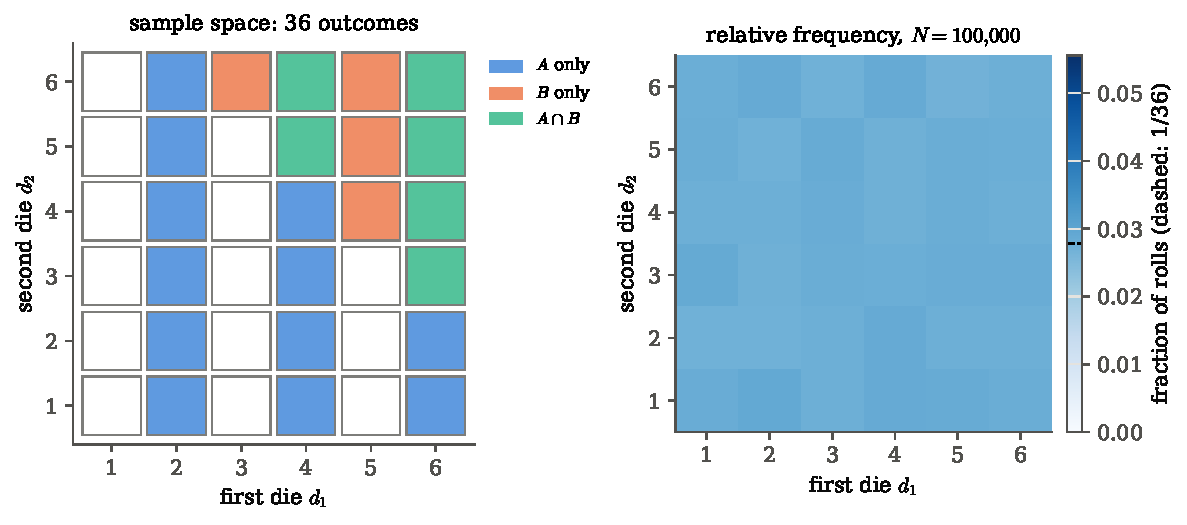
\includegraphics[width=\linewidth]{figures/ch01/1a_events_masks.pdf}
\caption{Left: the 36 outcomes of two dice as a grid, with the event $A$ (first
die even, blue), the event $B$ (sum at least 9, orange) and their overlap
(green). Counting cells gives the exact probabilities. Right: how often each
cell was hit in the simulation. Every cell is close to the dashed value $1/36$
on the colour bar, with small random differences.}
\label{1a:fig:events-masks}
\end{figure}

\paragraph{What this bought us.}
An event is a condition on outcomes, and in code it is a mask. Set identities
such as De Morgan's hold outcome by outcome, so they hold exactly for simulated
counts. Probabilities, which we define next, are what the frequencies of those
masks approach.

\section{The axioms of probability, and what they buy us}
\label{1a:sec:axioms}

Return to the three-paddle muon telescope of \cref{1a:ex:telescope}. Analyst
one has recorded a million muon passages and assigns to each of the eight
patterns the fraction of passages that produced it. Analyst two has just
installed a new middle paddle, has no data yet, and assigns numbers that
express how strongly she expects each pattern, based on the data sheet of the
photomultiplier. The two sets of numbers mean different things. Yet both
analysts will add them, subtract them from one, and combine them into trigger
probabilities in exactly the same way.

Whatever the numbers mean, any assignment of probabilities must obey three
rules, the axioms. Every rule we compute with follows from these three: the
complement rule, the inclusion--exclusion rule, the union bound that controls
the look-elsewhere effect, and the continuity that lets us take limits. Only
after the rules are in place do we ask what the numbers mean, and where each
meaning is used.

\paragraph{Probability is a unit of sand spread over the box.}
Take the box of possibilities from \cref{1a:sec:events} and pour exactly one
kilogram of sand over it, as unevenly as you like. The probability of an event
is the mass of sand lying inside its region. Mass is never negative. The whole
box holds all of it. If two regions do not overlap, the sand inside their union
is the sand in one plus the sand in the other. You would accept every one of
these statements about sand without proof. The proofs below only check that
three of them imply all the others.

\paragraph{What an assignment of probabilities must do.}
Stated in words, the demands are these.
\begin{enumerate}[leftmargin=1.5em,itemsep=1pt]
  \item To every event we can ask about, attach a number.
  \item The number for ``something happens'' ($\Omega$) must be the largest
        possible, and we fix the scale by calling it one.
  \item No event may get a negative number.
  \item Numbers for events that cannot happen together must add, also for an
        infinite list of such events.
  \item Everything else (complements, overlaps, limits) must then follow, so
        that we never need another rule.
\end{enumerate}

\begin{workdef}[probability distribution]
A \newterm{probability distribution} or \newterm{probability measure} $\Prob$
is a rule that assigns a real number $\Prob(A)$ to each event $A$
\unpack{each subset of $\Omega$ we are allowed to ask about, see
\cref{1a:sub:sigma}} such that
\begin{itemize}[leftmargin=1.2em,itemsep=1pt]
  \item[] \textbf{Axiom 1:} $\Prob(A)\ge 0$ for every event $A$.
  \item[] \textbf{Axiom 2:} $\Prob(\Omega)=1$.
  \item[] \textbf{Axiom 3:} if $A_1,A_2,\dots$ are disjoint
  \unpack{no outcome lies in two of them}, then
  \[
    \Prob\Bigl(\,\bigcup_{i=1}^\infty A_i\Bigr)=\sum_{i=1}^\infty \Prob(A_i).
  \]
\end{itemize}
Axiom 3 is called \newterm{countable additivity} \unpack{additivity for an
infinite sequence of disjoint events, one for each $i=1,2,3,\dots$}.
\emph{Operational test:} a table of numbers $\Prob(\{\omega\})$ on a finite or
countable $\Omega$ is a valid distribution exactly when every entry is
nonnegative and the entries sum to one.
\end{workdef}

These three lines are Kolmogorov's axioms (1933). They say nothing about
\emph{how} to find the numbers. That is the job of physics, of data and of
judgement. They only say which lists of numbers are internally consistent.

\subsection{Consequences of the axioms}

Five properties follow at once \mainref{p.~6, (1.1)}:
\begin{align}
&\Prob(\varnothing)=0, \nonumber\\
&A\subset B\ \Longrightarrow\ \Prob(A)\le\Prob(B), \nonumber\\
&0\le\Prob(A)\le 1, \label{1a:eq:props}\\
&\Prob(A^c)=1-\Prob(A), \nonumber\\
&A\cap B=\varnothing\ \Longrightarrow\ \Prob(A\cup B)=\Prob(A)+\Prob(B). \nonumber
\end{align}
Each takes a few lines to prove, and each proof is one idea that we will use
again, so we prove them all.

\paragraph{The empty event has probability zero.} Take the sequence
$A_1=\Omega$, $A_2=A_3=\cdots=\varnothing$. These are disjoint (the empty set
meets nothing) and their union is $\Omega$. Then
\begin{align*}
1 &\eqby{1} \Prob(\Omega)
   \eqby{2} \Prob\bigl(\Omega\cup\varnothing\cup\varnothing\cup\cdots\bigr)
   \eqby{3} \Prob(\Omega)+\sum_{i=2}^\infty\Prob(\varnothing)
   \eqby{4} 1+\sum_{i=2}^\infty\Prob(\varnothing).
\end{align*}
\begin{explain}
  \item Axiom 2.
  \item Adding empty sets to a union changes nothing.
  \item Axiom 3 for the disjoint sequence $\Omega,\varnothing,\varnothing,\dots$.
  \item Axiom 2 again.
\end{explain}
So $\sum_{i\ge2}\Prob(\varnothing)=0$. This is a sum of infinitely many copies
of the same number, which is nonnegative by Axiom 1. It is zero only if that
number is zero: $\Prob(\varnothing)=0$.

\paragraph{Finite additivity.} For disjoint $A_1,\dots,A_n$, pad the list with
empty sets, $A_{n+1}=A_{n+2}=\cdots=\varnothing$. Axiom 3 then gives
$\Prob(A_1\cup\cdots\cup A_n)=\sum_{i=1}^n\Prob(A_i)+\sum_{i>n}0$, which is the
last line of \eqref{1a:eq:props} for $n=2$.

\paragraph{Complement rule.} $A$ and $A^c$ are disjoint and $A\cup A^c=\Omega$, so
\begin{align}
1\eqby{1}\Prob(\Omega)\eqby{2}\Prob(A\cup A^c)\eqby{3}\Prob(A)+\Prob(A^c).
\label{1a:eq:complement}
\end{align}
\begin{explain}
  \item Axiom 2.
  \item Every outcome is either in $A$ or not.
  \item Finite additivity.
\end{explain}
This is the most used identity in the book: ``at least one'' is always
computed as one minus ``none''.

\paragraph{Monotonicity, and the difference rule.} If $A\subset B$, cut $B$
into the part inside $A$ and the part outside, $B=A\cup(B-A)$, which are
disjoint. Then
\begin{align}
\Prob(B)\eqby{1}\Prob(A)+\Prob(B-A)\relby{2}{\ge}\Prob(A).
\label{1a:eq:monotone}
\end{align}
\begin{explain}
  \item Finite additivity for the disjoint pieces $A$ and $B-A$.
  \item Axiom 1 for the event $B-A$.
\end{explain}
The first equality also says $\Prob(B-A)=\Prob(B)-\Prob(A)$ when $A\subset B$.
In detector language: a tighter cut $A$ inside a looser cut $B$ can only lose
outcomes, never gain them, so its probability cannot be larger. Finally
$0\le\Prob(A)$ is Axiom 1, and $\Prob(A)\le\Prob(\Omega)=1$ is monotonicity with
$B=\Omega$.

\begin{keyidea}[Inclusion--exclusion]
For any events $A$ and $B$,
\begin{equation}
\Prob(A\cup B)=\Prob(A)+\Prob(B)-\Prob(AB).
\label{1a:eq:incl-excl}
\end{equation}
Adding $\Prob(A)$ and $\Prob(B)$ counts the overlap twice, so we subtract it once.
\end{keyidea}

\begin{figure}[htbp]
\centering
\begin{tikzpicture}[scale=0.95]
  \coordinate (a) at (-0.8,0); \coordinate (b) at (0.8,0);
  \begin{scope}
    \fill[formblue!30] (a) circle (1.3);
    \fill[fibreorange!35] (b) circle (1.3);
    \begin{scope}\clip (a) circle (1.3); \fill[tangentgreen!40] (b) circle (1.3);\end{scope}
    \draw[thick] (-3,-1.8) rectangle (3,1.8);
    \draw (a) circle (1.3); \draw (b) circle (1.3);
    \node[lbl] at (-1.35,0) {$AB^c$};
    \node[lbl] at (0,0) {$AB$};
    \node[lbl] at (1.35,0) {$A^cB$};
    \node[lbl] at (-1.95,1.2) {$A$};
    \node[lbl] at (1.95,1.2) {$B$};
    \node[lbl] at (2.6,-1.45) {$\Omega$};
  \end{scope}
  \begin{scope}[xshift=7.0cm]
    \node[lbl,anchor=west] at (-2.4,1.2) {$\Prob(A)=\Prob(AB^c)+\Prob(AB)$};
    \node[lbl,anchor=west] at (-2.4,0.5) {$\Prob(B)=\Prob(AB)+\Prob(A^cB)$};
    \node[lbl,anchor=west] at (-2.4,-0.2) {sum: the green lens twice};
    \node[lbl,anchor=west] at (-2.4,-0.9) {$\Prob(A\cup B)$: each piece once};
  \end{scope}
\end{tikzpicture}
\caption{The union of two events is cut into three disjoint pieces: the part
of $A$ outside $B$ (blue), the overlap (green) and the part of $B$ outside $A$
(orange). $\Prob(A)$ and $\Prob(B)$ between them contain the green overlap
twice, and the union contains it once.}
\label{1a:fig:incl-excl}
\end{figure}

To prove \eqref{1a:eq:incl-excl}, use the three disjoint pieces of
\cref{1a:fig:incl-excl}: $A\cup B=(AB^c)\cup(AB)\cup(A^cB)$. Then
\begin{align*}
\Prob(A\cup B)
&\eqby{1} \Prob(AB^c)+\Prob(AB)+\Prob(A^cB)\\
&\eqby{2} \Prob(AB^c)+\Prob(AB)+\Prob(A^cB)+\Prob(AB)-\Prob(AB)\\
&\eqby{3} \Prob\bigl((AB^c)\cup(AB)\bigr)+\Prob\bigl((A^cB)\cup(AB)\bigr)-\Prob(AB)\\
&\eqby{4} \Prob(A)+\Prob(B)-\Prob(AB).
\end{align*}
\begin{explain}
  \item Finite additivity for three disjoint pieces.
  \item Add and subtract the same number.
  \item Finite additivity backwards, for the disjoint pairs $AB^c,AB$ and $A^cB,AB$.
  \item An outcome of $A$ is either outside $B$ or inside it, so
        $(AB^c)\cup(AB)=A$. Likewise $(A^cB)\cup(AB)=B$.
\end{explain}

\oneaEx{Two coin tosses}
\label{1a:ex:two-heads}
Let $H_1$ be ``heads on toss 1'' and $H_2$ ``heads on toss 2''. With the four
outcomes $HH,HT,TH,TT$ equally likely, $\Prob(H_1)=\Prob(\{HH,HT\})=\tfrac12$,
$\Prob(H_2)=\Prob(\{HH,TH\})=\tfrac12$ and $\Prob(H_1H_2)=\Prob(\{HH\})=\tfrac14$. So
\begin{align*}
\Prob(H_1\cup H_2)\eqby{1}\Prob(H_1)+\Prob(H_2)-\Prob(H_1H_2)
=\tfrac12+\tfrac12-\tfrac14=\tfrac34 .
\end{align*}
\begin{explain}
  \item Inclusion--exclusion \eqref{1a:eq:incl-excl}.
\end{explain}
Check by the complement rule: ``at least one head'' fails only for $TT$, so
the answer is $1-\tfrac14=\tfrac34$. The two routes must agree, and they do.

\oneaEx{A probability table for the telescope}
\label{1a:ex:telescope-probs}
On a finite sample space, finite additivity over single outcomes gives
\begin{equation}
\Prob(A)=\sum_{\omega\in A}\Prob(\{\omega\}),
\label{1a:eq:sum-atoms}
\end{equation}
so a distribution is just a table of nonnegative numbers that sum to one.
Suppose the telescope patterns have the probabilities
\begin{center}
\begin{tabular}{@{}lcccc@{}}
\toprule
pattern & $000$ & $001,\,010,\,100$ & $011,\,101,\,110$ & $111$\\
\midrule
probability (each) & $0.001$ & $0.009$ & $0.081$ & $0.729$\\
\bottomrule
\end{tabular}
\end{center}
They sum to $0.001+3(0.009)+3(0.081)+0.729=1$, so the table is legitimate.
(Where such numbers come from is the subject of \cref{1a:sec:independence}:
they are what one gets if each paddle fires with probability $0.9$ on its own.)
For the trigger $T$ and the event $U$ (top fired) of \cref{1a:ex:telescope-ops},
\begin{align*}
\Prob(T) &= 3(0.081)+0.729 = 0.972, \qquad \Prob(U)=0.009+2(0.081)+0.729=0.9,\\
\Prob(TU) &= \Prob(\{101,110,111\}) = 2(0.081)+0.729=0.891,\\
\Prob(T\cup U) &\eqby{1} 0.972+0.9-0.891 = 0.981 .
\end{align*}
\begin{explain}
  \item Inclusion--exclusion. Directly, $T\cup U=\{011,100,101,110,111\}$ has
        probability $0.081+0.009+0.081+0.081+0.729=0.981$, the same.
\end{explain}
The trigger misses a muon with probability $\Prob(T^c)=1-0.972=0.028$, by the
complement rule.

\paragraph{Try it: Three events.}
Show that
$\Prob(A\cup B\cup C)=\Prob(A)+\Prob(B)+\Prob(C)-\Prob(AB)-\Prob(AC)-\Prob(BC)+\Prob(ABC)$.
\emph{Hint:} apply \eqref{1a:eq:incl-excl} to $A\cup B$ and $C$, then use the
distributive law $(A\cup B)\cap C=(AC)\cup(BC)$ and \eqref{1a:eq:incl-excl}
once more, noting $(AC)(BC)=ABC$. In the telescope, the three events ``paddle
$j$ fired'' give $3(0.9)-3(0.81)+0.729=0.999$, which is $1-\Prob(\{000\})$.

\subsection{Two inequalities: Bonferroni and Boole}

Often we cannot compute an overlap $\Prob(AB)$, but we can still bound it from
below. Rearrange \eqref{1a:eq:incl-excl} and use $\Prob(A\cup B)\le 1$:
\begin{equation}
\Prob(AB)=\Prob(A)+\Prob(B)-\Prob(A\cup B)\ \ge\ \Prob(A)+\Prob(B)-1 .
\label{1a:eq:bonferroni}
\end{equation}
This is the simplest \newterm{Bonferroni inequality} \srcref{CasellaBerger}{(1.2.9)}.
\emph{Example.} The tracker and the calorimeter are each fully operational in
$95\%$ of the luminosity blocks. Then both are operational in at least
$95\%+95\%-100\%=90\%$ of them, however their failures are correlated. When
$\Prob(A)+\Prob(B)<1$ the bound is negative: true, but useless.

\begin{keyidea}[Boole's inequality, the union bound]
For any events $A_1,A_2,\dots$ (disjoint or not),
\begin{equation}
\Prob\Bigl(\,\bigcup_{n=1}^\infty A_n\Bigr)\le\sum_{n=1}^\infty\Prob(A_n).
\label{1a:eq:boole}
\end{equation}
The probability that at least one thing goes wrong is at most the sum of the
probabilities of each thing going wrong.
\end{keyidea}

Make the events disjoint by keeping only the part of each $A_n$ that is new:
$B_1=A_1$ and $B_n=A_n-\bigcup_{i<n}A_i$ \mainref{p.~14, Ex.~7}. An outcome in
$\bigcup_nA_n$ has a \emph{first} index $n$ with $\omega\in A_n$, and it lies in
$B_n$ for that $n$ only. So the $B_n$ are disjoint, $\bigcup_nB_n=\bigcup_nA_n$,
and $B_n\subset A_n$. Then
\begin{align*}
\Prob\Bigl(\,\bigcup_n A_n\Bigr)
\eqby{1}\Prob\Bigl(\,\bigcup_n B_n\Bigr)
\eqby{2}\sum_n\Prob(B_n)
\relby{3}{\le}\sum_n\Prob(A_n).
\end{align*}
\begin{explain}
  \item The two unions contain the same outcomes.
  \item Axiom 3 for the disjoint $B_n$.
  \item Monotonicity \eqref{1a:eq:monotone}, term by term, since $B_n\subset A_n$.
\end{explain}

\paragraph{In research: the look-elsewhere effect in one line.}
A bump hunt scans $m$ mass bins. If background alone makes a given bin
fluctuate up to the observed size with probability $\pval_{\text{local}}$, the
probability that \emph{some} bin does so is at most $m\,\pval_{\text{local}}$ by
\eqref{1a:eq:boole}. This is the Bonferroni correction for multiple tests
(\cref{ch:04}). It is a bound, and it is loose when neighbouring bins are
correlated. In real searches the actual ``global'' probability is obtained by
simulating many background-only experiments and counting how often the largest
fluctuation anywhere exceeds the observed one \cite{GrossVitells2010}. The
union bound is what tells us in advance roughly how bad the effect can be.

\oneaEx{Events of probability one}
\label{1a:ex:prob-one}
If $\Prob(A_i)=1$ for every $i$, then $\Prob\bigl(\bigcap_iA_i\bigr)=1$
\mainref{p.~14, Ex.~8}:
\begin{align*}
\Prob\Bigl(\bigl(\textstyle\bigcap_iA_i\bigr)^c\Bigr)
\eqby{1}\Prob\Bigl(\,\bigcup_iA_i^c\Bigr)
\relby{2}{\le}\sum_i\Prob(A_i^c)
\eqby{3}\sum_i 0 = 0 .
\end{align*}
\begin{explain}
  \item De Morgan's law \eqref{1a:eq:demorgan} for a countable family.
  \item Boole's inequality \eqref{1a:eq:boole}.
  \item Complement rule: $\Prob(A_i^c)=1-1=0$.
\end{explain}
A probability is nonnegative, so the complement has probability exactly zero
and the intersection has probability one. Countably many ``almost sure''
statements hold almost surely all at once.

\subsection{Continuity: probabilities of limits are limits of probabilities}

\paragraph{Continuity of probability.}
If $A_n\to A$ (a monotone sequence, \cref{1a:sec:events}), then
$\Prob(A_n)\to\Prob(A)$ as $n\to\infty$ \mainref{p.~7, Thm~1.8}.

\begin{figure}[htbp]
\centering
\begin{tikzpicture}[scale=0.9]
  \fill[formblue!12] (0,0) circle (2.2);
  \fill[formblue!30] (0,0) circle (1.6);
  \fill[formblue!55] (0,0) circle (1.0);
  \draw (0,0) circle (1.0); \draw (0,0) circle (1.6); \draw (0,0) circle (2.2);
  \draw[faint,dashed] (0,0) circle (2.55);
  \node[lbl,white] at (0,0) {$B_1=A_1$};
  \node[lbl] at (0,1.3) {$B_2$};
  \node[lbl] at (0,1.9) {$B_3$};
  \node[lbl,softgray] at (0,2.36) {$\cdots$};
  \draw[faint] (1.414,-1.686) -- (3.2,-2.2) node[lbl,anchor=west,black] {$A_3=B_1\cup B_2\cup B_3$};
  \draw[faint] (1.45,-0.676) -- (3.2,-1.2) node[lbl,anchor=west,black] {$A_2=B_1\cup B_2$};
  \draw[faint] (1.8,1.8) -- (3.2,1.8) node[lbl,anchor=west,black] {$A=\bigcup_nA_n$ (dashed)};
\end{tikzpicture}
\caption{An increasing sequence of events drawn as nested discs. The rings
$B_n$ (the part of $A_n$ that is new at step $n$) do not overlap, and the
first $n$ rings together make up $A_n$. The probability of the limit is the
total mass of all rings, which is the limit of the partial sums.}
\label{1a:fig:continuity}
\end{figure}

Suppose $A_1\subset A_2\subset\cdots$ with $A=\bigcup_iA_i$. Define the rings of
\cref{1a:fig:continuity}: $B_1=A_1$ and
$B_n=\{\omega:\ \omega\in A_n,\ \omega\notin A_{n-1}\}$ for $n\ge2$. Because the sets
are nested, ``not in $A_{n-1}$'' already means ``not in any earlier $A_i$'',
so this is the construction used for Boole's inequality. The $B_n$ are disjoint,
$A_n=\bigcup_{i=1}^nB_i$ and $\bigcup_{i=1}^\infty B_i=A$. Then
\begin{align*}
\lim_{n\to\infty}\Prob(A_n)
&\eqby{1}\lim_{n\to\infty}\Prob\Bigl(\,\bigcup_{i=1}^nB_i\Bigr)
 \eqby{2}\lim_{n\to\infty}\sum_{i=1}^n\Prob(B_i)
 \eqby{3}\sum_{i=1}^\infty\Prob(B_i)
 \eqby{4}\Prob\Bigl(\,\bigcup_{i=1}^\infty B_i\Bigr)
 \eqby{5}\Prob(A).
\end{align*}
\begin{explain}
  \item $A_n$ is the union of the first $n$ rings.
  \item Finite additivity.
  \item An infinite sum is by definition the limit of its partial sums. It
        converges because the partial sums increase and never exceed one.
  \item Axiom 3, which is where \emph{countable} additivity is essential.
  \item The rings together make up $A$.
\end{explain}
For a decreasing sequence $A_1\supset A_2\supset\cdots$ with $A=\bigcap_iA_i$, the
complements increase, $A_1^c\subset A_2^c\subset\cdots$, and by De Morgan
$\bigcup_iA_i^c=\bigl(\bigcap_iA_i\bigr)^c=A^c$. The increasing case gives
$\Prob(A_n^c)\to\Prob(A^c)$, so
$\Prob(A_n)=1-\Prob(A_n^c)\to1-\Prob(A^c)=\Prob(A)$ \mainref{p.~13, Ex.~1}.

\oneaEx{A detector that is alive forever}
\label{1a:ex:alive}
Let $A_n$ be ``the readout board has not failed during the first $n$ hours''.
The events decrease, $A_1\supset A_2\supset\cdots$, and their intersection $A$ is
``the board never fails''. Suppose a reliability model gives
$\Prob(A_n)=e^{-n/\tau}$ with a mean lifetime of $\tau=10^4$ hours. Continuity gives
\begin{align*}
\Prob(\text{never fails})\eqby{1}\lim_{n\to\infty}\Prob(A_n)=\lim_{n\to\infty}e^{-n/\tau}=0 .
\end{align*}
\begin{explain}
  \item Continuity for the decreasing sequence $A_n\to A$.
\end{explain}
We could not have computed $\Prob(A)$ directly, since $A$ is defined by an
infinite number of conditions. Continuity turns it into an ordinary limit.

\oneaEx{There is no uniform distribution on the integers}
\label{1a:ex:no-uniform-N}
Can we pick a whole number ``completely at random'', so that every
$n\in\{0,1,2,\dots\}$ has the same probability $c$ \mainref{p.~14, Ex.~6}? The
single-number events $\{0\},\{1\},\dots$ are disjoint with union $\Omega$, so
\begin{align*}
1\eqby{1}\Prob(\Omega)\eqby{2}\sum_{n=0}^\infty\Prob(\{n\})=\sum_{n=0}^\infty c
=\begin{cases}0 & c=0,\\ \infty & c>0.\end{cases}
\end{align*}
\begin{explain}
  \item Axiom 2.
  \item Axiom 3.
\end{explain}
Neither case equals one, so no such $\Prob$ exists. The same obstruction
appears for a ``flat prior'' on an unbounded parameter range, such as a
uniform distribution for a mass on $(0,\infty)$: it cannot be normalised.
Such an \emph{improper} prior can still be used as a device when the
posterior turns out normalisable, and \cref{ch:05} explains when.

\subsection{Which events are allowed? A word on $\sigma$-fields}
\label{1a:sub:sigma}

On a finite or countable $\Omega$ every subset can be an event. On $\R$ this
fails: one can prove that there is no way to give a ``length'' to
\emph{every} subset of $[0,1]$ that is countably additive and unchanged by
shifts. So probabilities are assigned only to a large, well-behaved class of
subsets \mainref{p.~13, \S1.9}.

\paragraph{$\sigma$-field, probability space.}
A \newterm{$\sigma$-field} (or $\sigma$-algebra) $\mathcal A$ is a collection
of subsets of $\Omega$ with (i) $\varnothing\in\mathcal A$, (ii) if
$A_1,A_2,\dots\in\mathcal A$ then $\bigcup_iA_i\in\mathcal A$, and (iii) if
$A\in\mathcal A$ then $A^c\in\mathcal A$ \unpack{the class of events is closed
under not, and countable or}. Its members are called \newterm{measurable}. The pair
$(\Omega,\mathcal A)$ is a \newterm{measurable space}, and with a probability
measure $\Prob$ on $\mathcal A$ the triple $(\Omega,\mathcal A,\Prob)$ is a
\newterm{probability space}. On $\R$ one uses the \newterm{Borel
$\sigma$-field}, the smallest $\sigma$-field containing all open intervals
\unpack{everything you can build from intervals by countably many unions,
intersections and complements}.

In practice this restriction never bites. Every event in this book
(intervals, histogram bins, excursion sets of a smooth field, limits of
monotone sequences) is Borel. A $\sigma$-field is also closed under countable
intersections, by De Morgan: $\bigcap_iA_i=\bigl(\bigcup_iA_i^c\bigr)^c$, and
the right side uses only complements and unions. So the limits of decreasing
sequences from \cref{1a:sec:events} stay inside it too.

\subsection{What the numbers mean: frequency and degree of belief}

The axioms fix the arithmetic. They do not say what $\Prob(A)=0.3$
\emph{means}. There are two standard answers \mainref{p.~6},
\srcref{Cowan}{\S1.2}, \srcref{Kruschke}{\S4.2}.

\begin{workdef}[frequency and degree-of-belief interpretations]
In the \newterm{frequency interpretation}, $\Prob(A)$ is the long-run proportion
of repetitions in which $A$ happens,
\begin{equation}
\Prob(A)=\lim_{n\to\infty}\frac{n_A}{n},
\label{1a:eq:freq}
\end{equation}
where $n_A$ is the \newterm{count} of $A$ \unpack{the number of runs, out of
$n$ identical and independent runs, in which $A$ occurred}.
In the \newterm{degree-of-belief} (subjective, Bayesian) interpretation,
$\Prob(A)$ measures how strongly a given observer, with given information,
believes that the statement $A$ is true. Here $\Omega$ is often called the
\newterm{hypothesis space} \unpack{a list of mutually exclusive statements,
exactly one of which is true}.
\end{workdef}

Both readings obey the same axioms, for different reasons. For frequencies
the axioms are automatic. A frequency is never negative, the frequency of
``some outcome'' is one, and the frequency of one of several disjoint outcomes
is the sum of their frequencies \srcref{Cowan}{p.~5}.

For beliefs the axioms are a consistency requirement, and a bet shows why.
Suppose you would pay $0.6$ for a ticket that pays $1$ if $A$ happens, and also
$0.6$ for a ticket that pays $1$ if $A$ does not. Buying both costs $1.2$.
Exactly one of the tickets wins, so you get back exactly $1$ whatever happens.
Your beliefs $\Prob(A)=\Prob(A^c)=0.6$ break the complement rule, and they lose
money for sure. Beliefs that cannot be exploited this way must obey the axioms.

The same kind of comparison pins a belief down. Suppose you prefer a ticket on
$A$ to a ticket on drawing red from a bag with 1 red and 9 white marbles. Then
your $\Prob(A)$ is above $0.1$. Suppose you also prefer a ticket on a bag with 5
red and 5 white to the ticket on $A$. Then your $\Prob(A)$ is below $0.5$. So it
lies between $0.1$ and $0.5$ \srcref{Kruschke}{\S4.2.2.1}.

The frequency reading needs repetition, so it fails for a unique object. It is
natural for anything that is repeated: collisions at a collider, photons in a
detector, the simulated universes of a Monte Carlo. Now take the electron mass
$m_e$. It is either inside the interval $[0.510,0.512]\,\text{MeV}$ or not, and
repeating the experiment does not change it. So the frequency of ``$m_e$ is in
the interval'' is either one (always inside) or zero (never), and we do not know
which. A statement like ``95\%
probability that $m_e$ lies in this interval'' only makes sense as a degree of
belief \srcref{Cowan}{p.~6}. The same is true of ``the probability that
$\Omega_m$ lies between $0.30$ and $0.32$'': there is one universe.

\begin{taxonomy}[Which interpretation, where in the book]
\begin{tabularx}{\linewidth}{@{}>{\raggedright}p{3.2cm}X@{}}
\toprule
\textbf{Frequency} & sampling distributions of data and statistics
(\cref{ch:02,ch:03}), $p$-values and the coverage of confidence intervals
(\cref{ch:04}), Monte Carlo error bars (\cref{ch:06}), cosmic variance of
$\Cell$ as scatter over hypothetical skies (\cref{ch:07}), the transfer
function and covariance of a masked pipeline (\cref{ch:08}).\\
\addlinespace
\textbf{Degree of belief} & priors and posteriors for parameters
$p(\params\given\data)$ (\cref{ch:05}), credible intervals from MCMC
(\cref{ch:09}), Fisher forecasts read as posterior widths (\cref{ch:10}),
systematic uncertainties.\\
\addlinespace
\textbf{Both, same rules} & everything in the theory of probability. The calculus is
shared, and in a Bayesian analysis the likelihood $\Prob(\data\given\params)$ is
itself a frequency statement about repeated data.\\
\bottomrule
\end{tabularx}
\end{taxonomy}

\subsection{A simulated long-run frequency}

The frequency definition \eqref{1a:eq:freq} is a limit, and a computer lets us
watch the limit being approached \mainref{p.~16, Ex.~21}. We flip a coin with
$\Prob(\text{heads})=p$ a thousand times and plot the proportion of heads so far.

\pyfile[firstline=23,lastline=34,firstnumber=23]{code/ch01/02_running_frequency.py}{Running proportion of heads}

Line 27 is the whole simulation: \texttt{rng.random(n\_max)} draws uniform
numbers in $[0,1)$, and a number lands below $p$ with probability $p$, so the
comparison is a coin with heads probability $p$. Line 28 divides the
cumulative count of heads by the number of flips so far, which is $n_A/n$ in
\eqref{1a:eq:freq}. Line 31 draws the band $p\pm2\sqrt{p(1-p)/n}$. Where that
width comes from is the variance of the binomial distribution in \cref{ch:02}.
For now it is simply a rule of thumb: at any given $n$, a run lies outside
the band only about one time in twenty.

\begin{figure}[htbp]
\centering
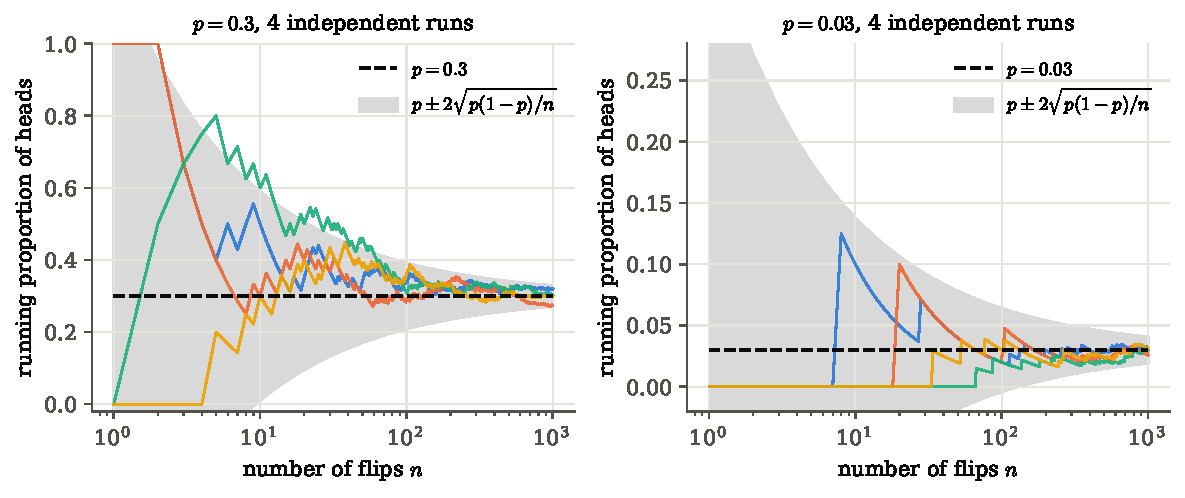
\includegraphics[width=\linewidth]{figures/ch01/1a_running_frequency.pdf}
\caption{Running proportion of heads for four independent runs of $1000$
flips, with $p=0.3$ (left) and $p=0.03$ (right). Early on the proportion jumps
around wildly. As flips accumulate the runs settle towards the dashed value,
and the shaded band $p\pm2\sqrt{p(1-p)/n}$ narrows like $1/\sqrt n$.}
\label{1a:fig:running}
\end{figure}

A rare event is harder to pin down than a common one. After $1000$ flips with
$p=0.3$, the first two runs end at $\OneARunFinalA$ and $\OneARunFinalAtwo$,
and $\OneARunInsideA$ of the $\OneARunRuns$ runs end inside the band
$0.3\pm\OneARunBandA$. With $p=0.03$ the first two end at $\OneARunFinalB$ and
$\OneARunFinalBtwo$, and $\OneARunInsideB$ of the $\OneARunRuns$ end inside
$0.03\pm\OneARunBandB$. The
band is narrower for the rare event in absolute terms. Relative to $p$, though,
it is much wider: about $10\%$ of $p$ for $p=0.3$, and almost $40\%$ of $p$ for
$p=0.03$. Dividing the half-width $2\sqrt{p(1-p)/n}$ by $p$ gives the relative
width $2\sqrt{(1-p)/(np)}$. It depends on $np$, the expected number of times the
event occurs. So estimating a small probability to a given relative precision
needs a number of trials proportional to $1/p$.

\paragraph{What this bought us.}
A finite run gives a frequency, not the probability. The frequency scatters
around the probability, and the scatter shrinks like $1/\sqrt{\text{(number of
occurrences)}}$. This is the first appearance of the Monte Carlo error, which
we will meet again every time a simulation estimates a number.

\begin{inpractice}[Verification here, instrument later]
Here we \emph{knew} $p$ and the simulation only verified that frequencies
approach it. In research the direction is reversed. Nobody can write down the
probability that a $pp$ collision at the LHC produces a muon that survives all
selection cuts. It is obtained exactly this way, as a frequency over millions
of simulated collisions, with the $1/\sqrt{n_A}$ scatter quoted as the
``Monte Carlo statistical uncertainty''.
\end{inpractice}

\paragraph{The frequency definition is not a recipe for every probability.}
Equation \eqref{1a:eq:freq} needs repeatable, identical runs. It gives no
meaning to $\Prob(\text{the Hubble tension is new physics})$. Conversely, a
degree of belief is not arbitrary: once it is written as a probability it must
obey all the rules above, and it must be updated by the rule of
\cref{1a:sec:bayes}.

\section{Equally likely outcomes: probability as counting}
\label{1a:sec:counting}

A silicon pixel sensor has $N=10^4$ pixels. In one readout frame, $k=100$
charged particles cross it, each landing on a pixel at random. If two particles
hit the same pixel, the pixel reports one hit, the two tracks share it, and the
tracking code may lose one of them. How often does at least one such merger
happen in a frame? The occupancy is only $100/10^4=1\%$, so one expects
``rarely''. The answer is about $39\%$.

When every outcome is equally likely, a probability is a ratio of two counts,
so all the work is in counting. Four basic counting formulas cover the cases:
ordered or not, with or without replacement. Physicists know them as
Maxwell--Boltzmann, Bose--Einstein and Fermi--Dirac counting. They settle the
pixel problem, which is the birthday problem in disguise, and we solve it three
ways: exactly, approximately and by simulation.

\paragraph{The microcanonical ensemble.}
In statistical mechanics an isolated system is equally likely to be in any of
its $\Omega(E)$ microstates of energy $E$. The probability of a macrostate is
then the number of microstates that realise it divided by $\Omega(E)$, and
entropy $S=k_B\ln\Omega$ is a logarithm of a count. Probability on a finite
sample space with equally likely outcomes is exactly this: fix the list of
equally likely microstates, and every probability is a ratio of counts.

\paragraph{Solving a counting problem.}
Every counting problem here is solved by the same four steps.
\begin{enumerate}[leftmargin=1.5em,itemsep=1pt]
  \item Find a sample space in which every outcome is equally likely. (This is
        a physical statement about the mechanism, not a counting fact.)
  \item Count all outcomes, $|\Omega|$.
  \item Count the outcomes in the event, $|A|$. Break the count into a
        sequence of simple choices.
  \item Divide. If counting $A$ is hard, count $A^c$ and use $1-|A^c|/|\Omega|$.
\end{enumerate}

\begin{workdef}[uniform distribution on a finite set]
If $\Omega=\{\omega_1,\dots,\omega_N\}$ is finite and every outcome has the
same probability, $\Prob(\{\omega_i\})=1/N$, then for every event
\begin{equation}
\Prob(A)=\frac{|A|}{|\Omega|}.
\label{1a:eq:uniform}
\end{equation}
This is the \newterm{uniform probability distribution} on $\Omega$
\unpack{probability of $A$ is the number of outcomes in $A$ over the number of
outcomes in $\Omega$}.
\emph{Operational test:} can you argue, from symmetry of the mechanism, that
no outcome is preferred? If not, \eqref{1a:eq:uniform} does not apply.
\end{workdef}

The equal value $1/N$ is forced: the $N$ single-outcome events are disjoint with
union $\Omega$, so $N\cdot c=1$. Then
\begin{align*}
\Prob(A)\eqby{1}\sum_{\omega\in A}\Prob(\{\omega\})\eqby{2}\sum_{\omega\in A}\frac1N
\eqby{3}\frac{|A|}{N}.
\end{align*}
\begin{explain}
  \item Finite additivity over the outcomes in $A$, \eqref{1a:eq:sum-atoms}.
  \item Every outcome has probability $1/N$.
  \item The sum has $|A|$ equal terms.
\end{explain}

\oneaEx{Two dice}
\label{1a:ex:two-dice}
Roll a die twice. $\Omega=\{(i,j):\ i,j\in\{1,\dots,6\}\}$ has $36$ ordered pairs,
all equally likely for fair dice rolled separately. The sum is $11$ for
$(5,6)$ and $(6,5)$, so $\Prob(\text{sum}=11)=2/36$. The sum is $7$ for $(1,6),(2,5),
\dots,(6,1)$, so $\Prob(\text{sum}=7)=6/36$. Here the pitfall of
\cref{1a:sec:events} bites: on the coarser space of sums $\{2,\dots,12\}$ the
eleven values are \emph{not} equally likely, and \eqref{1a:eq:uniform} would give
the wrong answer $1/11$.

\subsection{The multiplication principle}

\paragraph{Fundamental theorem of counting.}
If a job consists of $k$ separate choices, and the $i$-th choice can be made in
$n_i$ ways whatever the earlier choices were, the job can be done in
$n_1\times n_2\times\cdots\times n_k$ ways.

For $k=2$ choices, a table proves it. Write the possibilities with $n_1$ rows
(first choice) and $n_2$ columns (second choice). Each cell is one way of doing
the job, and there are $n_1n_2$ cells. For $k$ choices, treat the first $k-1$ as
one job and apply the $k=2$ case again and again. The phrase ``whatever the
earlier choices were'' matters. The \emph{number} of options at each step must
not depend on what was chosen before, although the options themselves may: when
dealing two cards, the second card has $51$ options whichever card came first,
but which $51$ depends on the first card.

\begin{figure}[htbp]
\centering
\begin{tikzpicture}[x=1.15cm,y=1cm]
  \foreach \i/\n in {1/{n},2/{n-1},3/{n-2}}{
    \draw[thick,formblue] (\i*1.6-0.6,0) rectangle (\i*1.6+0.6,0.8);
    \node[lbl] at (\i*1.6,0.4) {$\n$};
    \node[lbl,softgray] at (\i*1.6,-0.35) {slot \i};
  }
  \node[lbl] at (6.1,0.4) {$\cdots$};
  \draw[thick,formblue] (6.9,0) rectangle (8.5,0.8);
  \node[lbl] at (7.7,0.4) {$n-r+1$};
  \node[lbl,softgray] at (7.7,-0.35) {slot $r$};
  \node[lbl,anchor=west] at (0.9,-1.1) {ordered lists: $n(n-1)\cdots(n-r+1)=\dfrac{n!}{(n-r)!}$};
  \begin{scope}[yshift=-3.3cm]
    \foreach \w/\x in {abc/1.0,acb/2.0,bac/3.0,bca/4.0,cab/5.0,cba/6.0}{
      \node[draw=softgray,rounded corners=1pt,font=\small\ttfamily,inner sep=2pt] (w\w) at (\x,0.9) {\w};
    }
    \node[draw=fibreorange,thick,rounded corners=2pt,font=\small,inner sep=3pt] (set) at (3.5,-0.5) {$\{a,b,c\}$};
    \foreach \w in {abc,acb,bac,bca,cab,cba}{ \draw[faint] (w\w.south) -- (set.north); }
    \node[lbl,anchor=west] at (7.0,0.9) {$r!=6$ ordered lists};
    \node[lbl,anchor=west] at (7.0,-0.5) {one unordered set};
  \end{scope}
\end{tikzpicture}
\caption{Top: filling $r$ ordered slots from $n$ distinct objects without
putting any object back. The first slot has $n$ options, the second $n-1$, and
so on. Bottom: the $3!=6$ ordered lists of the letters $a,b,c$ all describe the
same unordered set, so counting sets means dividing the ordered count by $r!$.}
\label{1a:fig:slots}
\end{figure}

\paragraph{Permutations.} The number of ways to arrange $n$ distinct objects in
a row is $n!=n(n-1)\cdots2\cdot1$. Call it $P_n$. There are $n$ choices for the
first position, and then the remaining $n-1$ objects can be arranged in
$P_{n-1}$ ways, so $P_n=n\,P_{n-1}$ with $P_1=1$ \srcref{SeeingTheory}{p.~22}.
Unwinding the recursion gives $P_n=n!$. We set $0!=1$: there is exactly one way
to arrange nothing, and $P_1=1\cdot P_0$ requires $P_0=1$.

\paragraph{Ordered selection without replacement.} Filling $r$ ordered slots
from $n$ objects (\cref{1a:fig:slots}, top) can be done in
\begin{align*}
n(n-1)\cdots(n-r+1)\eqby{1}\frac{n(n-1)\cdots(n-r+1)\,(n-r)!}{(n-r)!}\eqby{2}\frac{n!}{(n-r)!}
\end{align*}
\begin{explain}
  \item Multiply and divide by $(n-r)!=(n-r)(n-r-1)\cdots1$.
  \item The numerator is now the full product $n(n-1)\cdots1$.
\end{explain}
ways, by the multiplication principle with $n_i=n-i+1$.

\paragraph{Unordered selection without replacement.} Now we want the number of
\emph{sets} of $r$ objects, ignoring order. Call it $\binom nr$. Every set of $r$
objects can be put in order in $r!$ ways (\cref{1a:fig:slots}, bottom), and every
ordered list arises from exactly one set. So we can count ordered lists in two
ways:
\begin{align}
\frac{n!}{(n-r)!}\eqby{1}\binom nr\times r!
\quad\Longrightarrow\quad
\binom nr=\frac{n!}{r!\,(n-r)!}.
\label{1a:eq:binom}
\end{align}
\begin{explain}
  \item Choose the set first ($\binom nr$ ways), then its order ($r!$ ways), and
        apply the multiplication principle.
\end{explain}
This is the \newterm{binomial coefficient}, read ``$n$ choose $r$''
\mainref{p.~8, (1.2)}. The method, counting something in two ways and
equating, is the most useful trick in combinatorics.

Two properties follow. $\binom n0=\binom nn=1$, since $0!=1$: there is one way
to choose nothing and one way to choose everything. And
$\binom nr=\binom n{n-r}$, since choosing the $r$ objects that are in is the same
as choosing the $n-r$ that are out. Algebraically, swapping $r\leftrightarrow n-r$
in $n!/(r!(n-r)!)$ swaps the two factorials in the denominator.

\oneaEx{Committees, and a poker hand}
\label{1a:ex:committee}
A class of $20$ elects a committee of $3$ \mainref{p.~8}:
\begin{align*}
\binom{20}{3}\eqby{1}\frac{20!}{3!\,17!}\eqby{2}\frac{20\times19\times18}{3\times2\times1}=1140 .
\end{align*}
\begin{explain}
  \item Definition \eqref{1a:eq:binom}.
  \item Cancel $17!$ from $20!=20\cdot19\cdot18\cdot17!$.
\end{explain}
A five-card poker hand is an unordered set of $5$ of $52$ cards, so there are
$\binom{52}5=2\,598\,960$ equally likely hands. ``Four aces'' fixes four cards and
leaves $48$ choices for the fifth, so $\Prob(\text{four aces})=48/2\,598\,960\approx
1.8\times10^{-5}$. ``Exactly one pair'' is built by a sequence of choices
\srcref{CasellaBerger}{(1.2.11)}: the pair's value ($13$ ways), its two suits
($\binom42=6$), the three other values, all different from each other and from
the pair ($\binom{12}3=220$), and a suit for each ($4^3=64$). So
\[
\Prob(\text{exactly one pair})=\frac{13\cdot6\cdot220\cdot64}{2\,598\,960}
=\frac{1\,098\,240}{2\,598\,960}\approx0.423 .
\]

\paragraph{Selection with replacement.} If an object is put back after being
chosen, every slot again has $n$ options, and there are $n^r$ ordered lists.

\paragraph{Unordered selection with replacement.} This is the hardest case.
An unordered choice of $r$ objects from $n$ types, repeats allowed, is fixed by
how many of each type we took. Draw the $n$ types as bins separated by $n-1$
walls, and each chosen object as a star in its bin (\cref{1a:fig:stars}). A
choice is then a row of $r$ stars and $n-1$ walls, and every such row is one
choice. Counting rows means choosing which $r$ of the $r+n-1$ positions hold
stars:
\begin{equation}
\#\{\text{unordered selections with replacement}\}=\binom{n+r-1}{r}.
\label{1a:eq:stars}
\end{equation}

\begin{figure}[htbp]
\centering
\begin{tikzpicture}[x=0.55cm,y=0.55cm]
  \foreach \x in {0,2,3,6}{ \node[font=\Large,fibreorange] at (\x,0) {$\star$}; }
  \foreach \x in {1,4,5}{ \draw[very thick,formblue] (\x,-0.7) -- (\x,0.7); }
  \draw[faint] (-0.8,-0.7) -- (-0.8,0.7); \draw[faint] (6.8,-0.7) -- (6.8,0.7);
  \node[lbl,anchor=north] at (0,-1.0) {1};
  \node[lbl,anchor=north] at (2.5,-1.0) {2};
  \node[lbl,anchor=north] at (4.5,-1.0) {3};
  \node[lbl,anchor=north] at (6,-1.0) {4};
  \node[lbl,softgray,anchor=north] at (3,-2.0) {bins (types or single-particle states)};
  \node[lbl,anchor=west] at (8.2,0.3) {occupations $(1,2,0,1)$};
  \node[lbl,anchor=west] at (8.2,-0.9) {$r=4$ stars, $n-1=3$ walls};
\end{tikzpicture}
\caption{Stars and bars. Four objects of four possible types are recorded as
a row of four stars and three walls. The stars between consecutive walls are
the objects of one type, so this row means one of type~1, two of type~2, none
of type~3 and one of type~4. The two outer walls (grey) never move and are not
counted.}
\label{1a:fig:stars}
\end{figure}

\begin{keyidea}[The four ways to choose $r$ objects from $n$]
\centering
\begin{tabular}{@{}lcc@{}}
\toprule
 & without replacement & with replacement\\
\midrule
ordered & $\dfrac{n!}{(n-r)!}$ & $n^r$\\[2ex]
unordered & $\dbinom nr$ & $\dbinom{n+r-1}{r}$\\
\bottomrule
\end{tabular}
\par\smallskip\raggedright
In the New York lottery ($6$ numbers from $44$) these are
$5\,082\,517\,440$, $7\,256\,313\,856$, $7\,059\,052$ and $13\,983\,816$ tickets
\srcref{CasellaBerger}{Table 1.2.1}.
\end{keyidea}

\paragraph{Counting in statistical mechanics.}
Put $r$ particles into $n$ single-particle states.
\begin{center}
\small
\begin{tabular}{@{}lll@{}}
\toprule
particles & counting & configurations\\
\midrule
distinguishable (Maxwell--Boltzmann) & ordered, with replacement & $n^r$\\
identical bosons (Bose--Einstein) & unordered, with replacement & $\binom{n+r-1}{r}$\\
identical fermions (Fermi--Dirac) & unordered, without replacement & $\binom nr$\\
\bottomrule
\end{tabular}
\end{center}
``With replacement'' means a state can hold more than one particle.
``Unordered'' means we only record occupation numbers, not which particle is where.

\begin{pitfall}[The count of outcomes is not a statement about their probabilities]
Take $r=2$ items from $n=3$ with replacement, by drawing, noting and putting
back. The nine ordered pairs are equally likely. The six unordered outcomes
$\{1,1\},\{2,2\},\{3,3\},\{1,2\},\{1,3\},\{2,3\}$ are \emph{not}: $\{1,2\}$ comes
from $(1,2)$ and $(2,1)$ and has probability $2/9$, while $\{1,1\}$ has $1/9$
\srcref{CasellaBerger}{Ex.~1.2.19}. Formula \eqref{1a:eq:stars} counts the
unordered outcomes, but only the mechanism decides which list is equally likely.
Physics gives a striking instance. For two particles in two states, the chance
that both sit in the same state is $1/2$ if they are distinguishable (states
$11,22$ out of $11,12,21,22$), $2/3$ for identical bosons (the three
occupations $(2,0),(1,1),(0,2)$ are the equally likely quantum states), and $0$
for fermions. That bosons ``bunch'' and fermions ``anti-bunch'' is measured
directly in Hanbury Brown--Twiss correlations. It is a fact about nature, not
about counting.
\end{pitfall}

\paragraph{Try it: Toss until two heads.}
A fair coin is tossed until the second head appears \mainref{p.~14, Ex.~5}.
Show that exactly $k$ tosses are needed with probability $(k-1)/2^k$ for
$k\ge2$. \emph{Answer:} every particular sequence of $k$ tosses has probability
$2^{-k}$. The event requires toss $k$ to be heads and exactly one head among the
first $k-1$ tosses, which can be placed in $\binom{k-1}{1}=k-1$ ways. As a check,
$\sum_{k\ge2}(k-1)2^{-k}=1$: differentiate $\sum_{k\ge0}x^k=1/(1-x)$ to get
$\sum_{k\ge1}kx^{k-1}=1/(1-x)^2$, and set $x=\tfrac12$ after multiplying by $x^2$.

\subsection{The birthday problem, and merged hits}

Now back to the pixel sensor from the start of this section: $N=10^4$ pixels,
$k=100$ particles per frame. Each of the $k$ particles lands on one of the $N$
pixels, independently and uniformly. (Independence is made precise in
\cref{1a:sec:independence}. Here it means that all $N^k$ ordered lists of
pixels, one entry per particle, are equally likely.) Let $D$ be the event ``at
least two particles share a pixel''. Its complement $D^c$, ``all $k$ pixels are
different'', is easier to count, because it is an ordered selection without
replacement.

\begin{align}
\Prob(D)
&\eqby{1} 1-\Prob(D^c)
 \eqby{2} 1-\frac{N(N-1)\cdots(N-k+1)}{N^k}
 \eqby{3} 1-\prod_{j=0}^{k-1}\Bigl(1-\frac jN\Bigr).
\label{1a:eq:bday-exact}
\end{align}
\begin{explain}
  \item Complement rule \eqref{1a:eq:complement}.
  \item Uniform distribution on the $N^k$ ordered lists (ordered, with
        replacement). $D^c$ contains the lists with all entries different
        (ordered, without replacement).
  \item Divide each of the $k$ factors $N-j$ of the numerator by one factor $N$
        of the denominator.
\end{explain}
For $N=365$ days this is the birthday problem. To see why the answer grows so
fast, take the logarithm and use $\ln(1-x)\approx-x$ for small $x$ (the first
term of the Taylor series $\ln(1-x)=-x-x^2/2-\cdots$):
\begin{align}
\ln\Prob(D^c)
&\eqby{1}\sum_{j=0}^{k-1}\ln\Bigl(1-\frac jN\Bigr)
 \relby{2}{\approx}-\sum_{j=0}^{k-1}\frac jN
 \eqby{3}-\frac{k(k-1)}{2N}.
\label{1a:eq:bday-approx}
\end{align}
\begin{explain}
  \item The logarithm of a product is the sum of the logarithms.
  \item $\ln(1-x)\approx-x$, valid when $j/N\ll1$, i.e.\ $k\ll N$.
  \item Arithmetic series, $0+1+\cdots+(k-1)=k(k-1)/2$.
\end{explain}
So $\Prob(D)\approx1-e^{-k(k-1)/2N}$. The exponent has a meaning: $k(k-1)/2=\binom k2$ is
the number of \emph{pairs} of particles, and each pair shares a pixel with
probability $1/N$. The number of pairs grows like $k^2$, which is why
coincidences come early. The probability reaches one half when
$k(k-1)/2N\approx\ln2$, i.e.\ $k\approx\sqrt{2N\ln2}\approx1.18\sqrt N$.

\oneaEx{Birthdays and pixels}
\label{1a:ex:birthday}
For $N=365$ and $k=23$, $\binom{23}2=253$ pairs, and \eqref{1a:eq:bday-exact}
gives $\Prob(D)=\OneABdayExact$, while the approximation gives
$1-e^{-253/365}=\OneABdayApprox$. The smallest group with better than even odds
has $k=\OneABdayKhalf$ people, close to $1.18\sqrt{365}\approx22.5$. With $50$
people the probability is $\OneABdayExactFifty$. For the pixel sensor, $N=10^4$
and $k=100$ give $\binom{100}{2}=4950$ pairs, and $\Prob(\text{some merged
hit})=\OneABdayPixExact$ exactly (approximation $\OneABdayPixApprox$), at a mean
occupancy of only $1\%$.

\pyfile[firstline=20,lastline=35,firstnumber=20]{code/ch01/03_birthday.py}{Exact, approximate and simulated birthday probabilities}

The exact function (lines 20--23) evaluates the product in
\eqref{1a:eq:bday-exact} as a product of numbers below one, which avoids the
enormous factorials. The simulation (lines 30--35) draws a $(\text{trials}\times k)$
array of random labels in $\{0,\dots,N-1\}$, one row per group. Sorting each row
puts equal labels next to each other, so a row contains a repeat exactly when
two neighbours are equal. The mean of that boolean column is the frequency of
$D$. With $200\,000$ simulated groups of $23$ the frequency is
$\OneABdayMC\pm\OneABdayMCErr$, and for $10^5$ simulated pixel frames it is
$\OneABdayPixMC\pm\OneABdayPixMCErr$. The error bars are the scatter
$\sqrt{q(1-q)/N}$ of a frequency. The two simulated values lie
$\OneABdayPull$ and $\OneABdayPixPull$ error bars from the exact ones.

\begin{figure}[htbp]
\centering
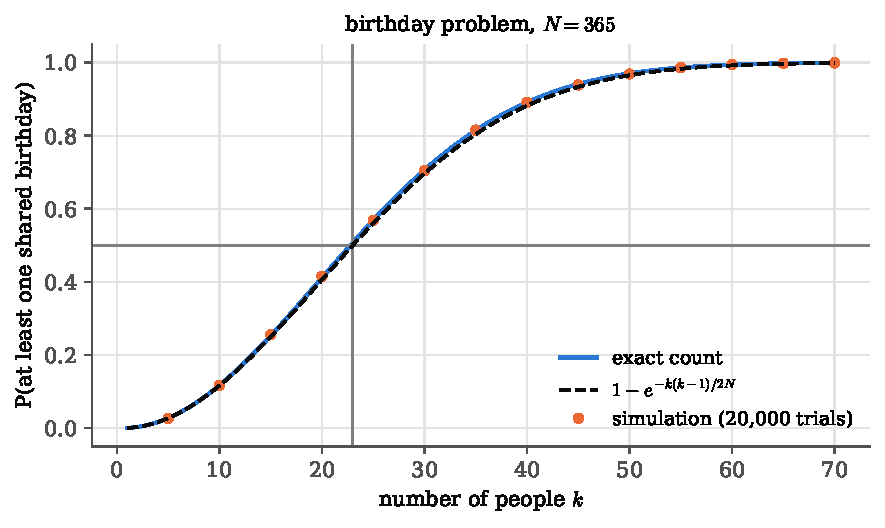
\includegraphics[width=0.8\linewidth]{figures/ch01/1a_birthday.pdf}
\caption{Probability that at least two of $k$ people share a birthday. The
exact count (solid) rises steeply and crosses one half between $22$ and $23$
people. The exponential approximation (dashed) lies just below it, and the
simulated frequencies (dots) fall on the exact curve.}
\label{1a:fig:birthday}
\end{figure}

\paragraph{What this bought us.}
Coincidences are governed by the number of \emph{pairs}, $\binom k2\approx k^2/2$,
not by $k$. A collision among $N$ equally likely labels becomes likely at
$k\sim\sqrt N$ draws, far below $N$.

\paragraph{In research: where the $\sqrt N$ rule bites.}
Pixel and strip detectors are designed so that occupancy stays low enough for
merged clusters to be rare, and the merging rate is estimated exactly as in
\cref{1a:ex:birthday}, then refined with a full simulation that includes the
real, non-uniform hit density near the beam. The same rule applies to random
seeds. If each of many parallel Monte Carlo jobs picks a $32$-bit seed at
random, two jobs share a seed (and produce identical ``independent'' samples)
with probability one half after only $1.18\sqrt{2^{32}}\approx77\,000$ jobs.
This is why \texttt{common.py} derives seeds deterministically through
\texttt{SeedSequence} (\cref{ch:06}).

\section{Conditional probability: shrinking the sample space}
\label{1a:sec:conditional}

At a collider, the trigger decides in microseconds which collisions are kept.
Everything an analyst later measures, such as the fraction of events with two
muons, the fraction whose muons have opposite charge or the fraction that fall
in a mass window, is a fraction \emph{among triggered events}. The events that
were not kept are gone. The analyst's world has shrunk from ``all collisions''
to ``collisions that fired the trigger''.

That is the whole idea: \emph{information shrinks the sample space}. The
question is this. Once we learn that an event $B$ happened, what is the new
probability of an event $A$? Conditional probability is the rule that answers
it, by computing probabilities inside the shrunken space. It is how a
probability changes when we learn something. Trees, the law of total
probability, independence and Bayes' theorem are all built from it. In a
simulation it is literally a selection: keep the rows in which $B$ holds, and
count among them.

In the area picture, conditioning changes only the unit of measurement.
Before we learn anything, $\Prob(A)$ is the fraction of the whole box $\Omega$
covered by $A$. If we learn that the outcome lies in $B$, every point outside
$B$ is ruled out, and $B$ becomes the new box. The probability of $A$ is now the
fraction of $B$ covered by $A$: the area of the overlap $AB$, measured in units
of the area of $B$ (\cref{1a:fig:shrink}). Nothing inside $B$ is re-weighted
relative to anything else inside $B$.

In \cref{1a:fig:shrink} the two regions are a hypothesis $H$ and an observed
event $E$. Their overlap $HE$ (green) can be measured against either one.
Measured against $H$, it is the share of the hypothesis region in which $E$
also happens. Measured against $E$, it is the share of the observed region in
which $H$ was also true. One patch, two yardsticks. Bayes' theorem
(\cref{1a:sec:bayes}) is the relation between those two readings of the same
patch, so the picture already contains it.

\begin{figure}[htbp]
\centering
\begin{tikzpicture}[scale=0.85]
  \begin{scope}
    \draw[thick] (0,0) rectangle (5,3.4);
    \fill[formblue!25] (0.5,0.5) rectangle (3.2,2.9);
    \fill[fibreorange!30] (2.2,0.9) rectangle (4.5,2.5);
    \fill[tangentgreen!45] (2.2,0.9) rectangle (3.2,2.5);
    \draw (0.5,0.5) rectangle (3.2,2.9);
    \draw (2.2,0.9) rectangle (4.5,2.5);
    \node[lbl] at (1.3,1.7) {$H$};
    \node[lbl] at (3.9,1.7) {$E$};
    \node[lbl] at (2.7,1.7) {$HE$};
    \node[lbl] at (4.6,3.05) {$\Omega$};
    \node[lbl,align=center] at (2.5,-0.55) {original sample space:\\ $\Prob(H)=\text{area}(H)/\text{area}(\Omega)$};
  \end{scope}
  \draw[->,thick,accent] (5.5,1.7) -- (6.9,1.7);
  \node[lbl,accent,anchor=south] at (6.2,2.3) {observe $E$};
  \begin{scope}[xshift=7.4cm]
    \draw[faint,dashed] (0,0) rectangle (5,3.4);
    \fill[fibreorange!30] (2.2,0.9) rectangle (4.5,2.5);
    \fill[tangentgreen!45] (2.2,0.9) rectangle (3.2,2.5);
    \draw[very thick,fibreorange] (2.2,0.9) rectangle (4.5,2.5);
    \node[lbl] at (2.7,1.7) {$HE$};
    \node[lbl] at (3.9,1.7) {$E$};
    \node[lbl,align=center] at (2.5,-0.55) {$E$ is the new reference space:\\ $\Prob(H\given E)=\text{area}(HE)/\text{area}(E)$};
  \end{scope}
\end{tikzpicture}
\caption{Conditioning as a change of reference space. Left: the hypothesis
region $H$ (blue) and the observed region $E$ (orange) overlap in the green
rectangle. Right: after we observe $E$, everything outside it is discarded and
the green area is measured as a fraction of the orange one. Measured against
$H$ instead, the same green area gives $\Prob(E\given H)$.}
\label{1a:fig:shrink}
\end{figure}

In words, computing a conditional probability takes four steps:
\begin{enumerate}[leftmargin=1.5em,itemsep=1pt]
  \item What do we know has happened? That event, $B$, is the new sample space.
  \item Discard every outcome outside $B$.
  \item Among the outcomes that remain, how much probability lies in $A$ as well?
  \item Rescale, so that the surviving outcomes carry total probability one.
\end{enumerate}
These four steps determine the formula completely. Write $\Prob_B(A)$ for the new
probability of $A$ once $B$ is known. We ask for three things: (i) $\Prob_B$ is a
probability, (ii) $\Prob_B(B)=1$, since $B$ is now certain, and (iii) inside $B$
nothing changes except the unit, $\Prob_B(C)=c\,\Prob(C)$ for every $C\subset B$,
with one constant $c$. Then for any event $A$,
\begin{align*}
\Prob_B(A)
&\eqby{1}\Prob_B(AB)+\Prob_B(AB^c)
 \eqby{2}\Prob_B(AB)
 \eqby{3}c\,\Prob(AB),
\qquad\text{and}\qquad
1\eqby{4}\Prob_B(B)\eqby{5}c\,\Prob(B).
\end{align*}
\begin{explain}
  \item $A$ is the disjoint union of its parts inside and outside $B$, and
        $\Prob_B$ is additive by (i).
  \item $AB^c\subset B^c$, and $\Prob_B(B^c)=1-\Prob_B(B)=0$ by (ii), so by
        monotonicity $\Prob_B(AB^c)=0$.
  \item $AB\subset B$, so (iii) applies.
  \item Requirement (ii).
  \item Requirement (iii) with $C=B$.
\end{explain}
The last equation fixes $c=1/\Prob(B)$, and the first gives
$\Prob_B(A)=\Prob(AB)/\Prob(B)$. There is no other choice.

\begin{workdef}[conditional probability]
If $\Prob(B)>0$, the \newterm{conditional probability of $A$ given $B$} is
\begin{equation}
\Prob(A\given B)=\frac{\Prob(AB)}{\Prob(B)}.
\label{1a:eq:cond}
\end{equation}
Read the bar as ``given'' \unpack{restricted to the outcomes in which $B$ is
true}. \emph{Frequency reading:} among the runs in which $B$ happened, the
fraction in which $A$ also happened, $\Prob(A\given B)\approx n_{AB}/n_B$
\unpack{$n_{AB}$ counts runs with both, $n_B$ runs with $B$, whatever $A$ did}.
\emph{Operational test in code:} \texttt{A[B].mean()}.
\end{workdef}

Three remarks. First, $\Prob(A)=\Prob(A\given\Omega)$: every probability is
conditional on the sample space we chose \srcref{Cowan}{p.~2}. Second, the
bar carries no arrow of time.
\[
\Prob(\text{rain last night}\given\text{wet ground this morning})
\]
is a perfectly good conditional probability: among mornings with wet ground,
the fraction that followed a rainy night
\srcref{Kruschke}{\S4.4.1}. Third, if $A$ and $B$ are disjoint then
$\Prob(A\given B)=0$: once $B$ has happened, $A$ cannot have.

\paragraph{The shrinking sample space, drawn to scale.}
Very often a problem does not hand us $\Prob(AB)$ directly. It tells us how
probable a situation $H$ is, and how often an observation $E$ occurs
\emph{inside} each situation. Take $\Prob(H)=0.25$, and suppose $E$ happens in
$60\%$ of the $H$-world and in $10\%$ of the $H^c$-world. This is the picture of
\cref{1a:fig:shrink} drawn to scale (\cref{1a:fig:area}). Draw $\Omega$ as a
rectangle of area one and $H$ as a vertical strip of width $0.25$. Inside each
strip, mark the part where $E$ happens as a piece running the full height of the
strip: it covers $0.6$ of the $H$ strip and $0.1$ of the $H^c$ strip. Set the two
pieces against the line between the strips, so that together they make one box,
the event $E$. The share of a strip that its piece covers is itself a
conditional probability: it is $E$ measured against the strip as its reference
space, so the two shares are $\Prob(E\given H)$ and $\Prob(E\given H^c)$.

Before we observe anything, $\Prob(H)$ is the width $0.25$ of the $H$ strip, a
fraction of the whole rectangle. Now learn that $E$ happened. Every point
outside the box is ruled out. The surviving region is the new sample space, and
probabilities are re-measured against its area:
\begin{align*}
\Prob(H\given E)
&\eqby{1}\frac{\text{area}(HE)}{\text{area}(E)}
 \eqby{2}\frac{\text{area}(HE)}{\text{area}(HE)+\text{area}(H^cE)}\\
&\eqby{3}\frac{0.25\times0.6}{0.25\times0.6+0.75\times0.1}
 =\frac{0.15}{0.225}=\frac23 .
\end{align*}
\begin{explain}
  \item Definition of conditional probability as re-measured area. The areas
        are probabilities because $\Omega$ has area one.
  \item $E$ is the union of its two pieces, which do not overlap because $H$ and
        $H^c$ are disjoint.
  \item Each piece is the strip's width times the share of the strip it
        covers, the width being the strip's probability and the share the
        conditional probability of $E$ inside the strip.
\end{explain}
Learning $E$ moved the probability of $H$ from $\tfrac14$ to $\tfrac23$. Why?
The figure shows it. The $H$ strip was only a third as wide as the $H^c$ strip
($0.25$ against $0.75$). But $E$ is six times as common inside $H$ as outside it
($0.6$ against $0.1$). So, of the area that survives, the $H$ piece ($0.15$) is
twice the $H^c$ piece ($0.075$), and $H$ holds two thirds of it.

Step (3) used the multiplication rule $\Prob(HE)=\Prob(E\given H)\Prob(H)$, read
off the picture here and derived as \eqref{1a:eq:mult} below. With every term
named, and the denominator written as a sum over all hypotheses, the same
calculation is Bayes' theorem (\cref{1a:sec:bayes} and \cref{ch:05}). Here it
is only the definition of conditional probability, drawn to scale.

\begin{figure}[htbp]
\centering
\begin{tikzpicture}[scale=0.8]
  \begin{scope}
    \fill[formblue!18] (0,0) rectangle (6,4);
    \fill[tangentgreen!45] (0.6,0) rectangle (1.95,4);
    \draw (1.5,0) -- (1.5,4);
    \draw[thick] (0,0) rectangle (6,4);
    \draw[line width=1.6pt,fibreorange] (0.6,0) rectangle (1.95,4);
    \node[lbl] at (0.3,2) {$H$};
    \node[lbl] at (3.975,2) {$H^c$};
    \node[lbl,font=\footnotesize] at (1.05,1.4) {$0.15$};
    \draw[faint] (1.75,2.6) -- (2.3,2.95) node[lbl,font=\footnotesize,anchor=south west,black,inner sep=1pt] {$0.075$};
    \node[lbl,fibreorange!80!black,anchor=south] at (1.275,4.05) {$E$};
    \node[lbl] at (6.25,3.75) {$\Omega$};
    \draw[faint] (0,-0.15) -- (0,-0.3) -- (1.5,-0.3) -- (1.5,-0.15);
    \draw[faint] (1.5,-0.15) -- (1.5,-0.3) -- (6,-0.3) -- (6,-0.15);
    \node[lbl] at (0.75,-0.6) {$0.25$};
    \node[lbl] at (3.75,-0.6) {$0.75$};
    \node[lbl,align=center,text width=6.2cm,anchor=north] at (3,-0.95) {before: $H$ fills a quarter of $\Omega$};
  \end{scope}
  \draw[->,thick,accent] (6.7,2) -- (8.1,2);
  \node[lbl,accent,align=center] at (7.4,2.75) {observe\\$E$};
  \begin{scope}[xshift=8.7cm]
    \draw[faint,dashed] (0,0) rectangle (6,4);
    \draw[faint,dashed] (1.5,0) -- (1.5,4);
    \fill[tangentgreen!45] (0.6,0) rectangle (1.95,4);
    \draw[very thin,black!40] (1.5,0) -- (1.5,4);
    \draw[line width=1.6pt,fibreorange] (0.6,0) rectangle (1.95,4);
    \node[lbl,align=center] at (1.05,2) {$H$\\[2pt]$\tfrac23$};
    \draw[faint] (1.75,1.2) -- (2.3,0.9) node[lbl,anchor=west,black,align=left,inner sep=1pt] {$H^c$: $\tfrac13$};
    \node[lbl,fibreorange!80!black,anchor=south] at (1.275,4.05) {$E$, area $0.225$};
    \node[lbl,align=center,text width=6.2cm,anchor=north] at (3,-0.95) {after: $E$ is the new sample space,\\ $H$ fills two thirds of it};
  \end{scope}
\end{tikzpicture}
\caption{Conditioning drawn to scale, in the picture of \cref{1a:fig:shrink}.
Left: the rectangle $\Omega$ has area 1, split into the strip $H$ of width
$0.25$ and the strip $H^c$ of width $0.75$. The event $E$ (orange outline)
covers $0.6$ of the $H$ strip and $0.1$ of the $H^c$ strip, so its two green
pieces have areas $0.25\times0.6=0.15$ and $0.75\times0.1=0.075$. Right: once
$E$ is observed, everything outside the orange box is discarded. $H$ keeps the
share of the box that its piece fills, $0.15/0.225=\tfrac23$, although its strip
was only a quarter of $\Omega$.}
\label{1a:fig:area}
\end{figure}

\oneaEx{Two dice, by counting in the shrunken space}
\label{1a:ex:dice-cond}
Roll two fair dice. Let $A$ be ``the sum is 8'' and $B$ ``at least one die shows
6''. By counting, $B$ has $11$ of the $36$ outcomes (six with a first 6, six with a
second 6, minus the double-counted $(6,6)$), $A=\{(2,6),(3,5),(4,4),(5,3),(6,2)\}$ has
$5$, and $AB=\{(2,6),(6,2)\}$ has $2$. Then
\begin{align*}
\Prob(A\given B)\eqby{1}\frac{\Prob(AB)}{\Prob(B)}\eqby{2}\frac{2/36}{11/36}=\frac{2}{11}\approx0.182,
\qquad
\Prob(B\given A)=\frac{2/36}{5/36}=\frac25=0.4 .
\end{align*}
\begin{explain}
  \item Definition \eqref{1a:eq:cond}.
  \item Uniform distribution on $36$ outcomes. The $1/36$ cancels, so the answer is
        a ratio of counts \emph{inside} $B$: $|AB|/|B|$.
\end{explain}
Learning $B$ raises the probability of $A$ from $5/36\approx0.139$ to $0.182$. The
two conditional probabilities use the same overlap and differ only in what it
is divided by.

\oneaEx{Hair and eye colour: reallocating credibility}
\label{1a:ex:hair-eye}
A sample of people has the joint proportions of eye and hair colour below
\srcref{Kruschke}{Table 4.1} (rows do not add exactly because of rounding in
the original data):
\begin{center}
\small
\begin{tabular}{@{}lccccc@{}}
\toprule
eye $\backslash$ hair & black & brunette & red & blond & marginal\\
\midrule
brown & 0.11 & 0.20 & 0.04 & 0.01 & 0.37\\
blue  & 0.03 & 0.14 & 0.03 & 0.16 & 0.36\\
hazel & 0.03 & 0.09 & 0.02 & 0.02 & 0.16\\
green & 0.01 & 0.05 & 0.02 & 0.03 & 0.11\\
\midrule
marginal & 0.18 & 0.48 & 0.12 & 0.21 & 1.0\\
\bottomrule
\end{tabular}
\end{center}
Learning ``blue eyes'' keeps only the second row and divides it by its total:
\begin{align*}
\Prob(\text{black}\given\text{blue})&=\tfrac{0.03}{0.36}=0.08, &
\Prob(\text{brunette}\given\text{blue})&=\tfrac{0.14}{0.36}=0.39,\\
\Prob(\text{red}\given\text{blue})&=\tfrac{0.03}{0.36}=0.08, &
\Prob(\text{blond}\given\text{blue})&=\tfrac{0.16}{0.36}=0.45 .
\end{align*}
The probability of blond hair rises from $0.21$ to $0.45$. The four numbers still
add up to one, because the row was divided by its own total. Learning ``blue
eyes'' has moved probability from some hair colours to others. Kruschke calls
this a reallocation of credibility. It is already Bayesian inference in
miniature.

\subsection{$\Prob(\cdot\given B)$ is a probability, $\Prob(A\given\cdot)$ is not}

For fixed $B$ with $\Prob(B)>0$, the function $A\mapsto\Prob(A\given B)$ satisfies the
three axioms \mainref{p.~14, Ex.~9}. Axiom 1 holds because a ratio of a
nonnegative number and a positive number is nonnegative. Axiom 2 holds because
$\Prob(\Omega\given B)=\Prob(\Omega B)/\Prob(B)=\Prob(B)/\Prob(B)=1$. For Axiom 3, let
$A_1,A_2,\dots$ be disjoint:
\begin{align*}
\Prob\Bigl(\,\bigcup_iA_i\,\Big\vert\, B\Bigr)
&\eqby{1}\frac{\Prob\bigl((\bigcup_iA_i)\cap B\bigr)}{\Prob(B)}
 \eqby{2}\frac{\Prob\bigl(\bigcup_i(A_iB)\bigr)}{\Prob(B)}
 \eqby{3}\frac{\sum_i\Prob(A_iB)}{\Prob(B)}
 \eqby{4}\sum_i\Prob(A_i\given B).
\end{align*}
\begin{explain}
  \item Definition \eqref{1a:eq:cond}.
  \item Distributive law \eqref{1a:eq:distrib}, for a countable family.
  \item The sets $A_iB$ are disjoint, because $A_iB\subset A_i$ and the $A_i$
        are. Then Axiom 3 for $\Prob$.
  \item Split the sum and use the definition for each term.
\end{explain}
So every rule of \cref{1a:sec:axioms} holds with ``$\given B$'' appended
everywhere: $\Prob(A^c\given B)=1-\Prob(A\given B)$, inclusion--exclusion, Boole.
This matters later, when all the machinery of probability is applied to a
posterior, which is a probability conditional on the data.

The same is \emph{not} true in the other slot. For fixed $A$, the map
$B\mapsto\Prob(A\given B)$ is not a probability. In general
$\Prob(A\given B\cup C)\neq\Prob(A\given B)+\Prob(A\given C)$, even for disjoint $B$ and
$C$. The quickest check: take $A=\Omega$, and any disjoint $B$ and $C$ of positive
probability. Every conditional probability of $\Omega$ is one, so the left side
is $1$ and the right side is $1+1=2$. The rules of probability act only on
events to the left of the bar \mainref{p.~10}.

\subsection{$\Prob(A\given B)$ is not $\Prob(B\given A)$}

The probability of spots given measles is essentially one. The probability of
measles given spots is small, since many things cause spots. The two
conditional probabilities share the numerator $\Prob(AB)$ and differ in the
denominator. \Cref{1a:fig:swap} draws it with the rectangles of
\cref{1a:fig:shrink}, now labelled $A$ and $B$. Conditioning on $B$ makes $B$
the whole world, and we ask what fraction of it the overlap fills. Swapping the
roles makes $A$ the whole world, and the same overlap is now measured against a
bigger region. In the picture the overlap has area $1.6$, $B$ has area $3.68$
and $A$ has area $6.48$, so
\begin{align*}
  \Prob(A\given B)&=\frac{\text{area}(AB)}{\text{area}(B)}=\frac{1.6}{3.68}=0.43,
  &
  \Prob(B\given A)&=\frac{\text{area}(AB)}{\text{area}(A)}=\frac{1.6}{6.48}=0.25 .
\end{align*}
Same patch, different yardstick, different answer. The two are equal only when
$A$ and $B$ have the same probability.

\begin{figure}[htbp]
\centering
\begin{tikzpicture}[scale=0.8]
  \begin{scope}
    \draw[faint,dashed] (0,0) rectangle (5,3.4);
    \draw[faint,dashed] (0.5,0.5) rectangle (3.2,2.9);
    \fill[fibreorange!30] (2.2,0.9) rectangle (4.5,2.5);
    \fill[tangentgreen!45] (2.2,0.9) rectangle (3.2,2.5);
    \draw[very thick,fibreorange] (2.2,0.9) rectangle (4.5,2.5);
    \node[lbl,softgray] at (1.3,1.7) {$A$};
    \node[lbl] at (2.7,1.7) {$AB$};
    \node[lbl] at (3.9,1.7) {$B$};
    \node[lbl,align=center] at (2.5,-0.6) {condition on $B$:\\ $\Prob(A\given B)=\text{area}(AB)/\text{area}(B)$};
  \end{scope}
  \begin{scope}[xshift=6.6cm]
    \draw[faint,dashed] (0,0) rectangle (5,3.4);
    \draw[faint,dashed] (2.2,0.9) rectangle (4.5,2.5);
    \fill[formblue!25] (0.5,0.5) rectangle (3.2,2.9);
    \fill[tangentgreen!45] (2.2,0.9) rectangle (3.2,2.5);
    \draw[very thick,formblue] (0.5,0.5) rectangle (3.2,2.9);
    \node[lbl] at (1.3,1.7) {$A$};
    \node[lbl] at (2.7,1.7) {$AB$};
    \node[lbl,softgray] at (3.9,1.7) {$B$};
    \node[lbl,align=center] at (2.5,-0.6) {condition on $A$:\\ $\Prob(B\given A)=\text{area}(AB)/\text{area}(A)$};
  \end{scope}
\end{tikzpicture}
\caption{Swapping what we condition on. The rectangles are those of
\cref{1a:fig:shrink}. Left: we learn that $B$ happened, so $B$ (orange outline)
is the new reference space and the green overlap is read as a fraction of
$B$. Right: we learn that $A$ happened instead, so $A$ (blue outline) is the
reference space and the same green overlap is read as a fraction of the larger
region $A$. Same numerator, different denominator: $\Prob(A\given B)=0.43$ but
$\Prob(B\given A)=0.25$.}
\label{1a:fig:swap}
\end{figure}

Mistaking one for the other is
common enough in court to have a name, the \newterm{prosecutor's fallacy}:
``the chance that an innocent person matches the DNA sample is one in a
million, so the chance that the defendant is innocent is one in a million''.
In statistics the same mistake reads ``$\Prob(\text{data this extreme}\given\Hnull)=0.01$,
so $\Prob(\Hnull\given\text{data})=0.01$'', which confuses a $p$-value with a
posterior probability (\cref{ch:04,ch:05}).

\oneaEx{A medical test}
\label{1a:ex:medical}
A test for a disease $D$ has outcomes $+$ and $-$, and the joint probabilities
are \mainref{p.~10, Ex.~1.13}
\begin{center}
\begin{tabular}{@{}lcc@{}}
\toprule
 & $D$ & $D^c$\\
\midrule
$+$ & $0.009$ & $0.099$\\
$-$ & $0.001$ & $0.891$\\
\bottomrule
\end{tabular}
\end{center}
Condition on the column (the true state) to get the test's performance:
\begin{align*}
\Prob(+\given D)\eqby{1}\frac{\Prob(+\cap D)}{\Prob(D)}\eqby{2}\frac{0.009}{0.009+0.001}=0.9,
\qquad
\Prob(-\given D^c)=\frac{0.891}{0.891+0.099}=0.9 .
\end{align*}
\begin{explain}
  \item Definition \eqref{1a:eq:cond}.
  \item $\Prob(D)$ is the sum of its column, since $D=(+\cap D)\cup(-\cap D)$ disjointly.
\end{explain}
The test is right $90\%$ of the time for the sick and for the healthy. Now
condition on the row (the result) instead:
\begin{align*}
\Prob(D\given +)\eqby{1}\frac{\Prob(+\cap D)}{\Prob(+)}\eqby{2}\frac{0.009}{0.009+0.099}
=\frac{9}{108}\approx0.08 .
\end{align*}
\begin{explain}
  \item Definition \eqref{1a:eq:cond}, now with $+$ as the conditioning event.
  \item $\Prob(+)$ is the sum of the first row.
\end{explain}
A positive result means the disease with probability $8\%$, not $90\%$. Among
positives, the healthy outnumber the sick eleven to one, because there are
ninety-nine times more healthy people to produce false positives
(\cref{1a:fig:dots}).

\begin{figure}[htbp]
\centering
\begin{tikzpicture}[x=0.24cm,y=0.24cm]
  \foreach \c in {0,...,49}{
    \foreach \r in {0,...,19}{
      \pgfmathtruncatemacro{\idx}{\c*20+\r}
      \ifnum\idx<9
        \fill[bdryred] (\c,-\r) circle (0.36);
      \else\ifnum\idx<10
        \draw[bdryred,thick] (\c,-\r) circle (0.30);
      \else\ifnum\idx<109
        \fill[fibreorange!70] (\c,-\r) circle (0.36);
      \else
        \fill[softgray!35] (\c,-\r) circle (0.30);
      \fi\fi\fi
    }
  }
  \node[lbl,anchor=west] at (0,-22.5)  {\tikz\fill[bdryred] (0,0) circle (3pt); sick, positive: 9};
  \node[lbl,anchor=west] at (0,-25)    {\tikz\draw[bdryred,thick] (0,0) circle (2.5pt); sick, negative: 1};
  \node[lbl,anchor=west] at (22,-22.5) {\tikz\fill[fibreorange!70] (0,0) circle (3pt); healthy, positive: 99};
  \node[lbl,anchor=west] at (22,-25)   {\tikz\fill[softgray!35] (0,0) circle (3pt); healthy, negative: 891};
  \node[lbl,anchor=west] at (40,-23.7) {$\Prob(D\given+)=\dfrac{9}{9+99}$};
\end{tikzpicture}
\caption{The medical test as a thousand people. The red dots at the top left
are the ten who are sick, nine of whom test positive. The orange block is the
ninety-nine healthy people who also test positive. Conditioning on a positive
result keeps only the filled coloured dots, and the red ones are a small
minority of them.}
\label{1a:fig:dots}
\end{figure}

\oneaEx{A radioactive nucleus does not age}
\label{1a:ex:nucleus}
A nucleus with decay constant $\lambda$ survives to time $t$ with probability
$\Prob(S_t)=e^{-\lambda t}$, where $S_t$ is ``not yet decayed at time $t$''. Given that
it has survived to $t$, what is the probability that it survives a further
time $s$? Surviving to $t+s$ implies surviving to $t$, so $S_{t+s}\subset S_t$ and
$S_{t+s}S_t=S_{t+s}$. Then
\begin{align*}
\Prob(S_{t+s}\given S_t)
\eqby{1}\frac{\Prob(S_{t+s}S_t)}{\Prob(S_t)}
\eqby{2}\frac{\Prob(S_{t+s})}{\Prob(S_t)}
\eqby{3}\frac{e^{-\lambda(t+s)}}{e^{-\lambda t}}
\eqby{4}e^{-\lambda s}=\Prob(S_s).
\end{align*}
\begin{explain}
  \item Definition \eqref{1a:eq:cond}.
  \item $S_{t+s}\subset S_t$.
  \item The survival law.
  \item $e^{a+b}=e^ae^b$.
\end{explain}
A nucleus that has already lived a thousand years is exactly as likely to
survive the next second as a freshly made one. The exponential law is the only
survival law with this \newterm{memoryless} property, and it is why the decay
constant is meaningful at all. Taking $s=\dd t$ small,
$\Prob(\text{decay in }[t,t+\dd t]\given S_t)=1-e^{-\lambda\,\dd t}\approx\lambda\,\dd t$: the decay
constant \emph{is} a conditional probability per unit time, the same at every
age. A human, or a photomultiplier tube, does age, and its survival law is not
exponential.

\subsection{The multiplication rule}

Multiplying \eqref{1a:eq:cond} by $\Prob(B)$, and doing the same with the roles of
$A$ and $B$ exchanged, gives the \newterm{multiplication rule}
\mainref{p.~11, Lemma~1.14}:
\begin{equation}
\Prob(AB)=\Prob(A\given B)\,\Prob(B)=\Prob(B\given A)\,\Prob(A).
\label{1a:eq:mult}
\end{equation}
Read it as a two-step story: for $A$ and $B$ both to happen, first $A$ must
happen, and then, in the world where $A$ has happened, $B$ must happen
\srcref{Lambert}{\S3.6}. Applying it repeatedly gives the \newterm{chain rule}
\mainref{p.~15, Ex.~17}:
\begin{align}
\Prob(ABC)
&\eqby{1}\Prob\bigl(A\given BC\bigr)\,\Prob(BC)
 \eqby{2}\Prob(A\given BC)\,\Prob(B\given C)\,\Prob(C),
\label{1a:eq:chain}
\end{align}
\begin{explain}
  \item Multiplication rule \eqref{1a:eq:mult} with the two events $A$ and $BC$.
  \item Multiplication rule again, for $\Prob(BC)$.
\end{explain}
and in general $\Prob(A_1A_2\cdots A_n)=\Prob(A_1)\Prob(A_2\given A_1)\Prob(A_3\given A_1A_2)\cdots
\Prob(A_n\given A_1\cdots A_{n-1})$. The chain rule is the arithmetic of a path through a
tree, which is the subject of the next section.

\oneaEx{Cards drawn without replacement}
\label{1a:ex:cards}
Draw two cards from a deck without putting the first back. Let $A$ be ``first is
the ace of clubs'' and $B$ ``second is the queen of diamonds''. Then
$\Prob(A)=1/52$, and once $A$ has happened the second card is uniform over the $51$
cards that remain, one of which is the queen of diamonds. So
$\Prob(AB)=\Prob(A)\Prob(B\given A)=\tfrac1{52}\cdot\tfrac1{51}$ \mainref{p.~11, Ex.~1.15}.

Four aces in a row: with $E_j$ ``the $j$-th card is an ace'',
\begin{align*}
\Prob(E_1E_2E_3E_4)
\eqby{1}\Prob(E_1)\Prob(E_2\given E_1)\Prob(E_3\given E_1E_2)\Prob(E_4\given E_1E_2E_3)
\eqby{2}\frac4{52}\cdot\frac3{51}\cdot\frac2{50}\cdot\frac1{49}
=\frac{1}{270\,725}.
\end{align*}
\begin{explain}
  \item Chain rule.
  \item At each step the shrunken deck is uniform: after $j$ aces, $52-j$ cards
        remain, $4-j$ of them aces.
\end{explain}
This equals $1/\binom{52}4$, as it must. Now condition on having started well
\srcref{CasellaBerger}{Ex.~1.3.3}. Given that the first $i$ cards are aces, the
deck has $52-i$ cards with $4-i$ aces, and the probability that the next $4-i$
cards are exactly those aces is $1/\binom{52-i}{4-i}$. For $i=1,2,3$ this is
$0.00005$, $0.00082$ and $0.0204$. Each piece of good news makes the event four
aces far more probable, though still unlikely.

\subsection{Conditioning is selection: a simulation}

In code, conditioning on $B$ means keeping only the rows where $B$ is true. We
repeat \cref{1a:ex:dice-cond} with $\OneACondN$ simulated rolls.

\pyfile[firstline=21,lastline=32,firstnumber=21]{code/ch01/04_conditioning_by_filtering.py}{Conditioning by filtering}

Lines 25--26 build the two masks. Line 29 is the whole of conditional
probability: \texttt{A[B]} is the sub-array of $A$ over the rows in which $B$
happened, and its mean is the fraction of those rows in which $A$ also
happened, $n_{AB}/n_B$. Line 32 computes the same number as a ratio of two
unconditional frequencies, $\hat\Prob(AB)/\hat\Prob(B)$, and the two agree exactly
($\OneACondAgB$ and $\OneACondRatio$), because $n_{AB}/n_B=(n_{AB}/N)/(n_B/N)$.

Of the $\OneACondN$ rolls, $\OneACondNB$ had at least one six, $\OneACondNA$ had
sum eight, and $\OneACondNAB$ had both. The estimates are
$\hat\Prob(A\given B)=\OneACondAgB$ (exact $2/11=\OneACondExAgB$) and
$\hat\Prob(B\given A)=\OneACondBgA$ (exact $2/5=\OneACondExBgA$).

\begin{figure}[htbp]
\centering
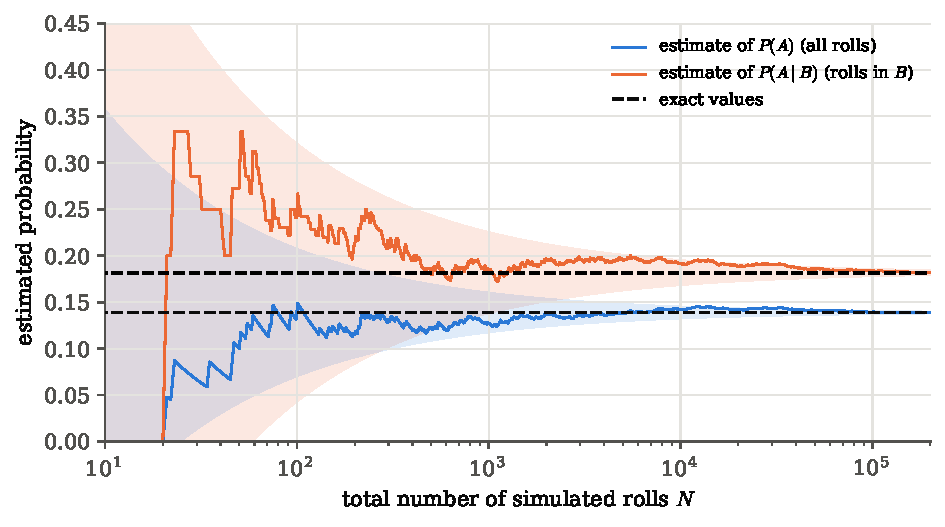
\includegraphics[width=0.85\linewidth]{figures/ch01/1a_conditioning.pdf}
\caption{Running estimates of $\Prob(A)$ from all rolls (blue) and of $\Prob(A\given B)$
from the rolls in $B$ only (orange), against the total number of simulated
rolls, with the exact values dashed. Both converge, but the conditional
estimate wanders more and its band is wider, because only about $30\%$ of the
rolls survive the selection.}
\label{1a:fig:conditioning}
\end{figure}

The figure shows the price of conditioning. The estimate of $\Prob(A\given B)$ uses
only $n_B\approx N\Prob(B)$ rolls, so its scatter is about
$\sqrt{\Prob(A\given B)(1-\Prob(A\given B))/(N\Prob(B))}$, the running-frequency rule of
\cref{1a:sec:axioms} with $n$ replaced by the number of survivors. Conditioning
on a rare event leaves few survivors, and then the estimate is noisy however
large $N$ was.

So conditioning is selection followed by renormalisation. In a simulation it
is one line, \texttt{A[B].mean()}, and its statistical error is set by how many
events survive the selection, not by how many were generated.

Two traps are worth naming. First, $\Prob(A\given B)$ and $\Prob(B\given A)$ are
different numbers, and they can be very different (\cref{1a:ex:medical}), so
always say in words which event is known. Second, \eqref{1a:eq:cond} needs
$\Prob(B)>0$. Conditioning on an event of probability zero, such as ``the
measured energy is exactly $91.1876$ GeV'', is still meaningful but needs
densities, which come in the next part.

\begin{inpractice}[Tag-and-probe]
The efficiency of a muon identification algorithm is a conditional
probability, $\Prob(\text{identified}\given\text{real muon})$. In data we do not know
which tracks are real muons, so we make a subset in which we do. Select
events with two tracks whose invariant mass is at the $Z$ peak and in which
one track (the ``tag'') passes a very tight identification. The other track
(the ``probe'') is then almost certainly a muon, and the fraction of probes
that pass the algorithm is the efficiency. The whole technique is the
definition \eqref{1a:eq:cond}, implemented as a selection on real events. Here
it is the research instrument: no formula gives this efficiency.
\end{inpractice}

Everything in this section comes back to one picture: the conditioning event
$B$ becomes the new, shrunk sample space \mainref{pp.~10--12, \S1.6}. It is
certain inside itself, $\Prob(B\given B)=\Prob(B)/\Prob(B)=1$
\srcref{CasellaBerger}{\S1.3}, and every other probability is re-measured as a
share of it (Seeing Theory draws the same idea as ``shelves'',
\srcref{SeeingTheory}{p.~27}). The medical test shows why we should not trust
intuition here: the shrunk space can hold a very different mix of cases from
the original one.
\section{Probability trees and the law of total probability}
\label{1a:sec:trees}

One collision in a hundred contains a real high-momentum muon ($S$, for
signal). The other $99\%$ do not ($B$, background). The hardware level-1
trigger (L1) fires for $95\%$ of the signal collisions and, because of fake
muons from hadrons punching through the calorimeter, for $2\%$ of the
background. The collisions that pass L1 are examined by the software
high-level trigger (HLT), which, \emph{among those that passed L1}, keeps
$90\%$ of the signal and $10\%$ of the background. What fraction of all
collisions is written to disk, and how much of what is written is signal?

A situation built from successive stages is drawn as a tree. Two rules then
answer both questions. The probability of each complete path is the product of
the conditional probabilities along it. The probability of an observation is
the sum over all the paths that lead to it. That sum is the law of total
probability. Read the right way, it is also marginalisation: averaging out the
stage we do not observe.

\paragraph{Water flowing through pipes.}
Pour one litre of water in at the root. At every junction the water divides
among the outgoing pipes in fixed proportions (the conditional probabilities),
and no water is lost, so the proportions at each junction add up to one. The
water reaching the end of a pipe is the product of the proportions along the
way. The total water collected in a bucket that several pipes drain into is
the sum of what each pipe delivers.

\paragraph{Building and reading a tree.}
The recipe, in words, is as follows.
\begin{enumerate}[leftmargin=1.5em,itemsep=1pt]
  \item What are the stages of the situation, in the order they are easiest
        to describe? (Nature picks $S$ or $B$, then L1 decides, then HLT decides.)
  \item At each node, what are the mutually exclusive possibilities for the
        next stage, and what is the probability of each \emph{given the path so far}?
  \item The probability of a complete path is the product along it.
  \item The probability of an event is the sum over the leaves where the event
        is true.
\end{enumerate}

\begin{workdef}[probability tree]
A \newterm{probability tree} is a rooted tree whose branches leaving each
node are the possible results of the next stage \unpack{mutually exclusive and
exhaustive, given everything above the node}. Each branch carries the
conditional probability of its result given the path from the root to its
node, so the labels leaving a node sum to one. A \newterm{path} from the root
to a leaf is one complete history, and the leaves partition $\Omega$
\unpack{every outcome follows exactly one path}.
\emph{Rules:} multiply along a path, add across paths.
\end{workdef}

\begin{figure}[htbp]
\centering
\begin{tikzpicture}[
  lev/.style={font=\small,inner sep=2pt},
  br/.style={thick,accent},
  pr/.style={font=\scriptsize,fill=white,inner sep=1pt},
  x=1cm,y=0.75cm]
  \node[lev] (r) at (0,0) {collision};
  \node[lev] (S) at (2.6,2.6) {$S$};
  \node[lev] (B) at (2.6,-2.6) {$B$};
  \node[lev] (SL) at (5.4,3.8) {L1};
  \node[lev] (SN) at (5.4,1.4) {no L1};
  \node[lev] (BL) at (5.4,-1.4) {L1};
  \node[lev] (BN) at (5.4,-3.8) {no L1};
  \node[lev] (SLH) at (8.2,4.6) {HLT};
  \node[lev] (SLN) at (8.2,3.0) {no HLT};
  \node[lev] (BLH) at (8.2,-0.6) {HLT};
  \node[lev] (BLN) at (8.2,-2.2) {no HLT};
  \draw[br] (r) -- node[pr,above left] {$0.01$} (S);
  \draw[br] (r) -- node[pr,below left] {$0.99$} (B);
  \draw[br] (S) -- node[pr,above left] {$0.95$} (SL);
  \draw[br] (S) -- node[pr,below left] {$0.05$} (SN);
  \draw[br] (B) -- node[pr,above left] {$0.02$} (BL);
  \draw[br] (B) -- node[pr,below left] {$0.98$} (BN);
  \draw[br] (SL) -- node[pr,above left] {$0.90$} (SLH);
  \draw[br] (SL) -- node[pr,below left] {$0.10$} (SLN);
  \draw[br] (BL) -- node[pr,above left] {$0.10$} (BLH);
  \draw[br] (BL) -- node[pr,below left] {$0.90$} (BLN);
  \node[font=\small,anchor=west,fibreorange] at (9.0,4.6) {$0.01\times0.95\times0.90=0.00855$};
  \node[font=\small,anchor=west,softgray] at (9.0,3.0) {$0.00095$};
  \node[font=\small,anchor=west,softgray] at (6.1,1.4) {$0.0005$};
  \node[font=\small,anchor=west,fibreorange] at (9.0,-0.6) {$0.99\times0.02\times0.10=0.00198$};
  \node[font=\small,anchor=west,softgray] at (9.0,-2.2) {$0.01782$};
  \node[font=\small,anchor=west,softgray] at (6.1,-3.8) {$0.9702$};
\end{tikzpicture}
\caption{The two-level trigger as a tree. The first split is nature's choice
between signal and background. Each later split is a trigger decision, and its
numbers are conditional on everything to the left. The numbers at the right
are the path probabilities, which add up to one. The two orange paths end in
``written to disk''.}
\label{1a:fig:trigger-tree}
\end{figure}

\subsection{Multiply along a path}

A path is an intersection of events, one per stage, so its probability is the
chain rule \eqref{1a:eq:chain}. For the top path of \cref{1a:fig:trigger-tree},
\begin{align}
\Prob(S\cap\mathrm{L1}\cap\mathrm{HLT})
&\eqby{1}\Prob(S)\,\Prob(\mathrm{L1}\given S)\,\Prob(\mathrm{HLT}\given S\cap\mathrm{L1})
 \eqby{2}0.01\times0.95\times0.90=0.00855 .
\label{1a:eq:path}
\end{align}
\begin{explain}
  \item Chain rule, with the events taken in the order of the stages.
  \item The branch labels. The last one is the HLT efficiency \emph{for signal
        that passed L1}, which is exactly how the HLT number was specified.
\end{explain}
The path probabilities at the right of \cref{1a:fig:trigger-tree} sum to one.
The reason is that the labels leaving each node sum to one. So the paths
through the branches leaving a node add up to the probability of the path
that reaches that node. Repeating this from the leaves back to the root leaves
the root's probability, one. In the water picture, no water is lost at a
junction.

\subsection{Add across paths: the law of total probability}

Let ``accepted'' be $\mathrm{Acc}=\mathrm{L1}\cap\mathrm{HLT}$. Two paths end in it,
one through $S$ and one through $B$. They are disjoint (a collision cannot be
both signal and background), so their probabilities add:
\begin{align*}
\Prob(\mathrm{Acc})=0.00855+0.99\times0.02\times0.10=0.00855+0.00198=0.01053 .
\end{align*}
About one collision in a hundred is kept. Nothing here was special to the
trigger: whenever the first stage splits $\Omega$ into disjoint pieces, the
probability of an event is the sum over the paths that end in it.

\begin{keyidea}[Law of total probability]
Let $A_1,\dots,A_k$ be a partition of $\Omega$. Then for any event $B$,
\begin{equation}
\Prob(B)=\sum_{i=1}^k\Prob(B\given A_i)\,\Prob(A_i).
\label{1a:eq:total}
\end{equation}
The first stage of the tree is the partition, the second stage is ``does $B$
happen'', and \eqref{1a:eq:total} adds the paths that end in $B$.
\end{keyidea}

To prove it, cut $B$ along the partition as in \cref{1a:fig:partition}:
$C_i=BA_i$. Every outcome of $B$ lies in exactly one $A_i$, so the $C_i$ are
disjoint and $B=\bigcup_iC_i$ \mainref{p.~12, Thm~1.16}. Then
\begin{align*}
\Prob(B)\eqby{1}\Prob\Bigl(\,\bigcup_iC_i\Bigr)\eqby{2}\sum_i\Prob(BA_i)\eqby{3}\sum_i\Prob(B\given A_i)\,\Prob(A_i).
\end{align*}
\begin{explain}
  \item $B$ is the union of its pieces $C_i$.
  \item Finite additivity for the disjoint pieces $C_i=BA_i$.
  \item Multiplication rule \eqref{1a:eq:mult} for each piece. If some
        $\Prob(A_i)=0$, the term $\Prob(BA_i)=0$ is simply dropped.
\end{explain}
The law holds just as well for a countable partition $A_1,A_2,\dots$, by
Axiom 3 in place of finite additivity.

\paragraph{Total probability is an average.}
The weights $\Prob(A_i)$ in \eqref{1a:eq:total} are nonnegative and sum to
one. So $\Prob(B)$ is a \emph{weighted average} of the conditional probabilities
$\Prob(B\given A_i)$, and it lies between the smallest and the largest of them.
In the trigger, the acceptance $0.01053$ lies between the background acceptance
$0.002$ ($=0.02\times0.10$) and the signal acceptance $0.855$
($=0.95\times0.90$). It sits very close to the background value, because
background carries $99\%$ of the weight.

This averaging is what it means to \newterm{marginalise}. We average out the
stage we do not observe, here the true nature of the collision. That stage
plays the role of a \emph{nuisance} variable: it matters for the answer, but we
do not ask about it. In \cref{ch:05} the same sum becomes an integral over
parameters $\params$ given data $\data$,
$p(\data)=\int p(\data\given\params)\,p(\params)\,\dd\params$, the evidence.

\oneaEx{The 662 keV line of caesium-137}
\label{1a:ex:cs137}
A $^{137}$Cs nucleus $\beta$-decays either to the excited isomer $^{137m}$Ba
(probability about $0.944$) or directly to the ground state of $^{137}$Ba (about
$0.056$). The isomer de-excites by emitting a $662$ keV photon with probability
about $0.902$. Otherwise the energy is carried off by an internal-conversion
electron. The direct branch emits no $662$ keV photon. The probability that one
decay produces a $662$ keV photon is
\begin{align*}
\Prob(\gamma_{662})
&\eqby{1}\Prob(\gamma_{662}\given{}^{137m}\mathrm{Ba})\,\Prob({}^{137m}\mathrm{Ba})
       +\Prob(\gamma_{662}\given\text{ground})\,\Prob(\text{ground})\\
&\eqby{2}0.902\times0.944+0\times0.056\approx0.851 ,
\end{align*}
\begin{explain}
  \item Law of total probability over the two decay branches.
  \item Branch probabilities from the nuclear data tables.
\end{explain}
which is the ``$85.1\%$ gamma intensity'' printed in the tables. A third stage,
``the photon deposits its full energy in the detector'' with probability
$\varepsilon$, multiplies the useful path by $\varepsilon$. A source of activity
$\mathcal A$ (decays per second) therefore gives a photopeak rate
$0.851\,\varepsilon\mathcal A$. Every calibration with a radioactive source uses
this tree.

\oneaEx{A coin from a bag}
\label{1a:ex:bag-total}
A bag holds a fair coin and a coin with $\Prob(\text{heads})=0.95$. We pick one
blindly and toss it three times \srcref{SeeingTheory}{p.~27}. Let $F$ be ``fair
coin picked'' and $H_3$ ``three heads''. Given the coin, the tosses are
independent (\cref{1a:sec:independence}), so $\Prob(H_3\given F^c)=0.95^3=0.857$ and
$\Prob(H_3\given F)=0.5^3=0.125$. Then
\begin{align*}
\Prob(H_3)\eqby{1}\Prob(H_3\given F^c)\Prob(F^c)+\Prob(H_3\given F)\Prob(F)
=0.857\times0.5+0.125\times0.5\approx0.491 .
\end{align*}
\begin{explain}
  \item Law of total probability over the partition $\{F,F^c\}$.
\end{explain}
We will reverse this tree in \cref{1a:sec:bayes} to ask which coin we hold.

\oneaEx{Taking turns: a tree with infinitely many paths}
\label{1a:ex:basketball}
Two players take turns shooting at a basket, player 1 first. Player 1 scores
with probability $1/3$, player 2 with probability $1/4$, independently each
time. What is the probability that player 1 scores first
\mainref{p.~9, Ex.~1.11}?

\begin{center}
\begin{tikzpicture}[x=1.45cm,y=0.9cm,
  br/.style={thick,accent},pr/.style={font=\scriptsize,fill=white,inner sep=1pt},
  nd/.style={font=\small,inner sep=2pt}]
  \node[nd] (a0) at (0,0) {start};
  \node[nd,fibreorange] (w1) at (1,-1.3) {1 scores};
  \node[nd] (m1) at (1,0) {1 misses};
  \node[nd,softgray] (l1) at (2,-1.3) {2 scores};
  \node[nd] (m2) at (2,0) {2 misses};
  \node[nd,fibreorange] (w2) at (3,-1.3) {1 scores};
  \node[nd] (m3) at (3,0) {1 misses};
  \node[nd,softgray] (l2) at (4,-1.3) {2 scores};
  \node[nd] (m4) at (4,0) {2 misses};
  \node[nd] (dots) at (5,0) {$\cdots$};
  \draw[br] (a0) -- node[pr,left] {$\tfrac13$} (w1);
  \draw[br] (a0) -- node[pr,above] {$\tfrac23$} (m1);
  \draw[br] (m1) -- node[pr,left] {$\tfrac14$} (l1);
  \draw[br] (m1) -- node[pr,above] {$\tfrac34$} (m2);
  \draw[br] (m2) -- node[pr,left] {$\tfrac13$} (w2);
  \draw[br] (m2) -- node[pr,above] {$\tfrac23$} (m3);
  \draw[br] (m3) -- node[pr,left] {$\tfrac14$} (l2);
  \draw[br] (m3) -- node[pr,above] {$\tfrac34$} (m4);
  \draw[br,dashed] (m4) -- (dots);
\end{tikzpicture}
\end{center}
Let $A_j$ be ``the first basket is by player 1, on her $j$-th attempt''. Each
$A_j$ is one path: $j-1$ rounds of ``both miss'', then player 1 scores. The
$A_j$ are disjoint and their union is the event $E$ we want. Each round of
two misses has probability $\tfrac23\cdot\tfrac34=\tfrac12$, so
$\Prob(A_j)=(\tfrac12)^{j-1}\tfrac13$, and
\begin{align*}
\Prob(E)\eqby{1}\sum_{j=1}^\infty\Prob(A_j)
\eqby{2}\frac13\sum_{j=1}^\infty\Bigl(\frac12\Bigr)^{j-1}
\eqby{3}\frac13\cdot\frac{1}{1-\tfrac12}=\frac23 .
\end{align*}
\begin{explain}
  \item Axiom 3, since the paths $A_j$ are disjoint.
  \item Multiply along each path.
  \item Geometric series, $\sum_{m=0}^\infty r^m=1/(1-r)$ for $0\le r<1$. It follows
        from $(1-r)(1+r+\cdots+r^{M})=1-r^{M+1}$ and $r^{M+1}\to0$. More generally
        $\sum_{j=k}^\infty r^j=r^k/(1-r)$.
\end{explain}
A shortcut avoids the series. Look only at the first round. With probability
$\tfrac13$ player 1 scores at once. With probability $\tfrac12$ both miss, and then
the game starts afresh, so player 1 scores first with probability $\Prob(E)$
again. In the remaining case player 2 scored. So
$\Prob(E)=\tfrac13+\tfrac12\Prob(E)$, which again gives $\Prob(E)=\tfrac23$.

\paragraph{Try it: Until both faces have appeared.}
Toss a fair coin until both a head and a tail have appeared
\mainref{p.~15, Ex.~13}. The sample space is
$\{HT,TH,HHT,TTH,HHHT,TTTH,\dots\}$. Show that exactly three tosses are needed
with probability $1/4$. \emph{Answer:} two paths, $HHT$ and $TTH$, each of
probability $(1/2)^3$.

\subsection{Following each collision down the tree}

The trigger tree can be simulated literally: generate the nature of each
collision, then each trigger decision with the probability appropriate to
that branch.

\pyfile[firstline=24,lastline=39,firstnumber=24]{code/ch01/05_trigger_chain.py}{The trigger tree, exactly and by simulation}

Lines 25--28 are the tree read as arithmetic: multiply along the two accepted
paths and add them. Line 33 is nature's choice at the root. Line 34 is the L1
split: \texttt{np.where} uses the signal efficiency on signal rows and the
background efficiency on background rows, which is precisely what
``conditional on the branch'' means. Line 35 applies the HLT only to rows that
passed L1 (the \texttt{l1 \&}), again with a branch-dependent efficiency. Lines
37--38 count the accepted collisions separately on each path. Line 39 is a
preview of \cref{1a:sec:bayes}: among accepted collisions, the fraction that is
signal.

With $2\times10^6$ simulated collisions, $\OneATrigNacc$ are accepted, a
frequency of $\OneATrigMCAcc$ against the exact $\OneATrigAcc$. The signal path
contributes $\OneATrigMCPathS$ (exact $\OneATrigPathS$) and the background path
$\OneATrigMCPathB$ (exact $\OneATrigPathB$).

\begin{figure}[htbp]
\centering
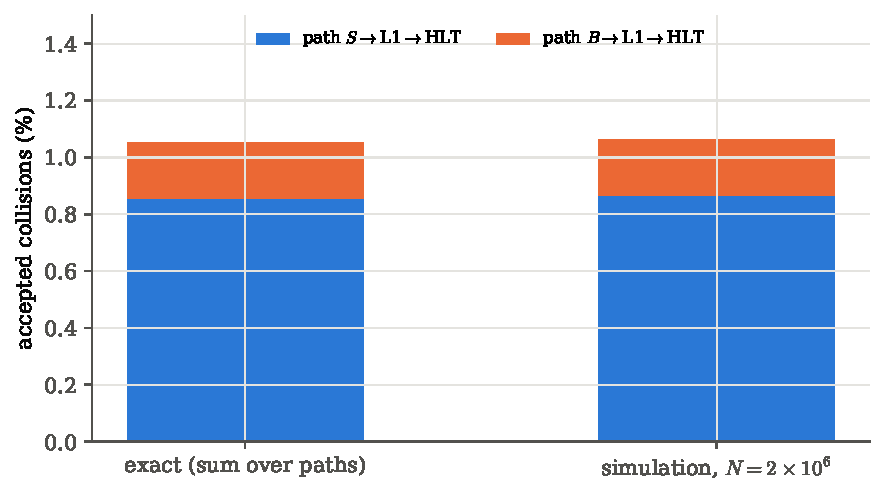
\includegraphics[width=0.75\linewidth]{figures/ch01/1a_trigger_chain.pdf}
\caption{The fraction of collisions written to disk, split into the two paths
of the tree that lead there. The left bar is the exact sum over paths, the
right bar the simulation. Signal (blue) supplies most of the accepted
collisions although only one collision in a hundred is signal.}
\label{1a:fig:trigger-bars}
\end{figure}

\paragraph{What this bought us.}
A tree turns a many-stage problem into bookkeeping: conditional probabilities
on the branches, products along paths, sums across paths. The law of total
probability is the sum across the paths that end in the observed event, and
it is a weighted average of the branch-wise probabilities.

\paragraph{In research: trigger rates and emulation.}
In a real experiment each trigger level has a rate budget (for example
$100$~kHz out of L1 and a few kHz out of the HLT), and the total rate is computed
exactly as a sum over the physics processes that can fire it, each weighted by
its cross section: the law of total probability with the processes as the
partition. Here the simulation only verified the tree. In practice the
branch efficiencies depend on the momentum, angle and pile-up of each
collision, and no closed formula exists. One then runs the trigger emulation
on millions of simulated events and counts, so the simulation is the
instrument and the tree is the check that one understands the result.

\begin{pitfall}[Branch labels are conditional on the path]
Two traps. First, the HLT keeps $90\%$ of signal \emph{that passed L1}. That is
$\Prob(\mathrm{HLT}\given S\cap\mathrm{L1})$, not $\Prob(\mathrm{HLT}\given S)$ and certainly not
$\Prob(\mathrm{HLT})$. Multiplying unconditional probabilities along a path is correct
only when the stages are independent, which is the subject of the next section.
Second, the paths that are added must be disjoint. The leaves of a tree always
are, which is why drawing the tree is safer than adding probabilities by eye.
\end{pitfall}

\section{Independence: when learning $B$ tells us nothing about $A$}
\label{1a:sec:independence}

In \cref{1a:ex:telescope-probs} we used a table in which the pattern $111$ had
probability $0.729=0.9^3$ and each pattern with one silent paddle had
$0.081=0.9^2\times0.1$. Those numbers come from one assumption: each paddle fires
with probability $0.9$ \emph{whatever the other paddles do}. The paddles are
separate pieces of plastic with separate photomultipliers, so this is
plausible. It fails if the three tubes share a high-voltage supply that
sometimes sags, because then one silent paddle makes it more likely that the
others are silent too.

Independence is the precise version of ``whatever the others do''. It is the
one situation in which the probability of ``$A$ and $B$'' is the product of the
two probabilities. That product rule lets us write the probability of a data
set as a product over data points, and every likelihood in this book is built
that way. There are two things that independence is not. First, independence is not the same as disjointness. Second, when there are three or more events, independence does not mean merely that every pair of events is independent.

\paragraph{Crossed strips.}
Draw $\Omega$ as the unit square. Let $A$ be a vertical strip of width
$\Prob(A)$ and $B$ a horizontal strip of height $\Prob(B)$. Their overlap is a
rectangle of area $\Prob(A)\Prob(B)$. Inside $A$, the strip $B$ covers the same
fraction $\Prob(B)$ as it covers of the whole square, so learning ``$A$
happened'' does not change the probability of $B$. Independence is this
product structure. Two dice, two separate detectors or two separate nuclei
behave like the two axes of the square.

\begin{figure}[htbp]
\centering
\begin{tikzpicture}[scale=1.25]
  \begin{scope}
    \draw[thick] (0,0) rectangle (2.4,2.4);
    \fill[formblue!30] (0,0) rectangle (1.2,2.4);
    \fill[fibreorange!30] (0,1.6) rectangle (2.4,2.4);
    \fill[tangentgreen!50] (0,1.6) rectangle (1.2,2.4);
    \draw (1.2,0) -- (1.2,2.4); \draw (0,1.6) -- (2.4,1.6);
    \node[lbl] at (0.6,0.8) {$A$};
    \node[lbl] at (1.8,2.0) {$B$};
    \node[lbl] at (0.6,2.0) {$AB$};
    \node[lbl] at (1.2,-0.35) {independent};
  \end{scope}
  \begin{scope}[xshift=3.2cm]
    \draw[thick] (0,0) rectangle (2.4,2.4);
    \fill[formblue!30] (0,0) rectangle (1.2,2.4);
    \fill[fibreorange!30] (1.2,1.6) rectangle (2.4,2.4);
    \fill[fibreorange!30] (1.2,0) rectangle (2.4,0.8);
    \draw (1.2,0) -- (1.2,2.4); \draw (1.2,1.6) -- (2.4,1.6); \draw (1.2,0.8) -- (2.4,0.8);
    \node[lbl] at (0.6,1.2) {$A$};
    \node[lbl] at (1.8,2.0) {$B$};
    \node[lbl] at (1.8,0.4) {$B$};
    \node[lbl] at (1.2,-0.35) {disjoint};
  \end{scope}
  \begin{scope}[xshift=6.4cm]
    \draw[thick] (0,0) rectangle (2.4,2.4);
    \fill[formblue!30] (0,0) rectangle (1.2,2.4);
    \fill[fibreorange!30] (1.2,2.0) rectangle (2.4,2.4);
    \fill[tangentgreen!50] (0,1.2) rectangle (1.2,2.4);
    \draw (1.2,0) -- (1.2,2.4);
    \draw (0,1.2) -- (1.2,1.2);
    \draw (1.2,2.0) -- (2.4,2.0);
    \node[lbl] at (0.6,0.6) {$A$};
    \node[lbl] at (1.8,2.2) {$B$};
    \node[lbl] at (0.6,1.8) {$AB$};
    \node[lbl] at (1.2,-0.35) {dependent};
  \end{scope}
\end{tikzpicture}
\caption{Three ways for two events to sit in the unit square, all drawn to scale and
all with $\Prob(A)=\tfrac12$ (the left half) and $\Prob(B)=\tfrac13$. Left: $B$ is the
top third, so it fills a third of $A$ and a third of the square, and $\Prob(AB)=\tfrac16$,
exactly the product: independent. Middle: $A$ and $B$ do not meet, so $\Prob(AB)=0$ and
knowing $A$ rules $B$ out. Right: $B$ still has area $\tfrac13$ but leans into $A$, so
$\Prob(AB)=\tfrac14\neq\tfrac16$. The two overlaps have the same width, so compare their
heights: $B$ covers half of $A$ on the right but only a third of $A$ on the left. Covering
more of $A$ than its $\tfrac13$ share of the square, $B$ becomes more likely once we learn $A$.}
\label{1a:fig:independence}
\end{figure}

\paragraph{Checking independence.}
Whenever a calculation seems to need independence, we ask four questions.
\begin{enumerate}[leftmargin=1.5em,itemsep=1pt]
  \item In words: does knowing that $B$ happened change how likely $A$ is?
  \item In numbers: is $\Prob(AB)$ equal to $\Prob(A)\Prob(B)$?
  \item Is independence being \emph{assumed} (no physical mechanism links the
        two) or \emph{derived} (computed from a known distribution)?
  \item For more than two events, check every sub-collection, not just the pairs.
\end{enumerate}

\begin{workdef}[independence]
Two events $A$ and $B$ are \newterm{independent}, written $A\perp\!\!\!\perp B$, if
\begin{equation}
\Prob(AB)=\Prob(A)\,\Prob(B).
\label{1a:eq:indep}
\end{equation}
A collection $\{A_i:\ i\in I\}$ is \newterm{independent} (or \newterm{mutually
independent}) if
$\Prob\bigl(\bigcap_{i\in J}A_i\bigr)=\prod_{i\in J}\Prob(A_i)$ for \emph{every} finite
subset $J\subseteq I$ \unpack{for three events that means the three pairs and the
triple, four equations in all}. Otherwise the events are dependent.
\emph{Operational test:} with $\Prob(B)>0$, independence is $\Prob(A\given B)=\Prob(A)$.
\end{workdef}

The conditional form is the meaning, and the product form is the convenient
definition, because it is symmetric and also makes sense when $\Prob(B)=0$. They
agree whenever $\Prob(B)>0$ \mainref{p.~11, Lemma~1.14}:
\begin{align*}
\Prob(A\given B)\eqby{1}\frac{\Prob(AB)}{\Prob(B)}\eqby{2}\frac{\Prob(A)\Prob(B)}{\Prob(B)}=\Prob(A),
\end{align*}
\begin{explain}
  \item Definition of conditional probability.
  \item Independence \eqref{1a:eq:indep}.
\end{explain}
and conversely, if $\Prob(A\given B)=\Prob(A)$ then multiplying by $\Prob(B)$ gives
\eqref{1a:eq:indep}. By the symmetry of \eqref{1a:eq:indep}, $\Prob(B\given A)=\Prob(B)$ too
when $\Prob(A)>0$: if $B$ tells us nothing about $A$, then $A$ tells us nothing about
$B$.

\paragraph{Assumed or derived.} Often independence is an \emph{assumption} that
expresses physics: a coin has no memory of its last toss, two nuclei do not
communicate, the noise in two separate amplifiers has separate sources.
Sometimes it is a \emph{result} \mainref{p.~8}. Roll one fair die and let
$A=\{2,4,6\}$ and $B=\{1,2,3,4\}$. Then $AB=\{2,4\}$ and
\[
\Prob(AB)=\tfrac26=\tfrac13=\tfrac12\times\tfrac23=\Prob(A)\Prob(B),
\]
so $A$ and $B$ are independent, although both are about the same single roll.
Nobody assumed it. With $C=\{4,5,6\}$ instead, $AC=\{4,6\}$ and
$\Prob(AC)=\tfrac13\neq\tfrac12\times\tfrac12$: knowing the roll is high makes it more
likely to be even.

\subsection{Consequences}

\paragraph{Complements of independent events are independent.}
If $A\perp\!\!\!\perp B$,
\begin{align*}
\Prob(AB^c)\eqby{1}\Prob(A)-\Prob(AB)\eqby{2}\Prob(A)-\Prob(A)\Prob(B)\eqby{3}\Prob(A)\bigl(1-\Prob(B)\bigr)
\eqby{4}\Prob(A)\Prob(B^c).
\end{align*}
\begin{explain}
  \item $A$ is the disjoint union of $AB$ and $AB^c$, so $\Prob(A)=\Prob(AB)+\Prob(AB^c)$.
  \item Independence of $A$ and $B$.
  \item Factor out $\Prob(A)$.
  \item Complement rule.
\end{explain}
So $A\perp\!\!\!\perp B^c$ \mainref{p.~15, Ex.~11}, \srcref{CasellaBerger}{Thm~1.3.9}. Applying the same argument with the roles of the events
exchanged gives $A^c\perp\!\!\!\perp B^c$. If a paddle's firing tells us nothing
about another's, neither does its silence.

\paragraph{Sure and impossible events are independent of everything}
\mainref{p.~15, Ex.~14}. If $\Prob(A)=0$, then $\Prob(AB)\le\Prob(A)=0$ by
monotonicity, so $\Prob(AB)=0=\Prob(A)\Prob(B)$. If $\Prob(A)=1$, then $\Prob(A^c)=0$, so $A^c$
is independent of every $B$, and by the complement result so is $A$. Finally,
an event independent of itself satisfies $\Prob(A)=\Prob(AA)=\Prob(A)^2$, so
$\Prob(A)\in\{0,1\}$.

\begin{keyidea}[Disjoint is not independent]
If $A$ and $B$ are disjoint and both have positive probability, they are
\emph{dependent}: $\Prob(A)\Prob(B)>0$, but $\Prob(AB)=\Prob(\varnothing)=0$
\mainref{p.~9}. Disjoint events are as dependent as events can be: learning
that one happened tells us for certain that the other did not.
\end{keyidea}

Apart from this case, a Venn diagram cannot show independence. Whether the
overlap equals the product depends on the areas, not on the shapes. In
\cref{1a:fig:independence} the right panel looks as ``overlapping'' as the left
one, yet only the left is independent.

Two more warnings \srcref{Lambert}{\S3.4}. First, take a playing card. Its
colour and its suit are dependent: ``red'' forces hearts or diamonds. Its suit
and its value are independent: $\Prob(\heartsuit\given\text{queen})=\tfrac14=\Prob(\heartsuit)$.
Second, dependence is not causation. The colour does not \emph{cause} the suit.
Dependence only means that knowing one tells us something about the other.

\subsection{Examples}

\oneaEx{At least one head in ten tosses}
\label{1a:ex:ten-tosses}
Let $A$ be ``at least one head'' in ten tosses of a fair coin and $T_j$ ``tails on
toss $j$'' \mainref{p.~9, Ex.~1.10}. Then
\begin{align*}
\Prob(A)&\eqby{1}1-\Prob(A^c)\eqby{2}1-\Prob(T_1T_2\cdots T_{10})
\eqby{3}1-\Prob(T_1)\Prob(T_2)\cdots\Prob(T_{10})\eqby{4}1-\Bigl(\frac12\Bigr)^{10}\approx0.999 .
\end{align*}
\begin{explain}
  \item Complement rule.
  \item ``No head'' means ``tails on every toss''.
  \item The tosses are independent (assumed: the coin has no memory).
  \item Each factor is $\tfrac12$.
\end{explain}
The Chevalier de M\'er\'e's bet ``at least one six in four rolls of a die'' is
the same computation, $1-(5/6)^4\approx0.518$ \srcref{CasellaBerger}{Ex.~1.3.8}, a
slightly favourable bet. His other bet, ``at least one double six in $24$ rolls of
two dice'', gives $1-(35/36)^{24}\approx0.491$, slightly unfavourable, which puzzled
him enough to write to Pascal.

\oneaEx{Telescope efficiency, and the first decay in a sample}
\label{1a:ex:indep-physics}
\emph{(a)} Each paddle fires with probability $\varepsilon$, independently. The
trigger needs at least two paddles. The pattern $111$ has probability
$\varepsilon^3$, and each of the three patterns with exactly one silent paddle
has probability $\varepsilon^2(1-\varepsilon)$, by the product rule for the three
independent events ``paddle $j$ fired or not'' (complements are independent
too). So
\begin{align*}
\Prob(T)\eqby{1}3\varepsilon^2(1-\varepsilon)+\varepsilon^3=3\varepsilon^2-2\varepsilon^3,
\end{align*}
\begin{explain}
  \item Finite additivity over the four disjoint patterns in $T$.
\end{explain}
which is $0.972$ at $\varepsilon=0.9$, reproducing the table of
\cref{1a:ex:telescope-probs}. A two-out-of-three majority turns $90\%$ paddles into
a $97\%$ trigger.

\emph{(b)} A sample holds $N$ nuclei, each surviving to time $t$ with probability
$e^{-\lambda t}$ (\cref{1a:ex:nucleus}), independently of the others. The
probability that \emph{none} has decayed by $t$ is
\begin{align*}
\Prob\Bigl(\,\bigcap_{i=1}^NS^{(i)}_t\Bigr)\eqby{1}\prod_{i=1}^N\Prob\bigl(S^{(i)}_t\bigr)
=\bigl(e^{-\lambda t}\bigr)^N=e^{-N\lambda t}.
\end{align*}
\begin{explain}
  \item Mutual independence of the $N$ survival events.
\end{explain}
``None has decayed by $t$'' is the same event as ``the first decay comes after
$t$''. So the waiting time until the first click of a Geiger counter has the
survival law $e^{-N\lambda t}$ of a single nucleus with rate $N\lambda$: it is
itself exponential, with rate $N\lambda$, the activity of the sample. This is
the seed of the Poisson process of \cref{ch:02}.

\oneaEx{Blue eyes}
\label{1a:ex:blue-eyes}
Each of three children has blue eyes with probability $\tfrac14$, independently
\mainref{p.~15, Ex.~15}. Let $K$ be the number of blue-eyed children.
\emph{(a)} Given that at least one has blue eyes, what is the probability that at
least two do? The event $\{K\ge2\}$ lies inside $\{K\ge1\}$, so
\begin{align*}
\Prob(K\ge2\given K\ge1)\eqby{1}\frac{\Prob(K\ge2)}{\Prob(K\ge1)}
\eqby{2}\frac{3\cdot\tfrac1{16}\cdot\tfrac34+\tfrac1{64}}{1-\bigl(\tfrac34\bigr)^3}
=\frac{10/64}{37/64}=\frac{10}{37}\approx0.27 .
\end{align*}
\begin{explain}
  \item Definition of conditional probability, with $\{K\ge2\}\cap\{K\ge1\}=\{K\ge2\}$.
  \item Numerator: exactly two blue (three choices of the brown-eyed child) or
        all three. Denominator: complement of ``none blue''. Independence gives
        each pattern's probability as a product.
\end{explain}
\emph{(b)} Given that the \emph{youngest} has blue eyes, at least two are blue-eyed
exactly when at least one of the other two is. By independence the youngest
tells us nothing about them, so the answer is $1-(\tfrac34)^2=\tfrac7{16}\approx0.44$.
The two conditions sound alike but carry different information, and (b) is
the larger because it pins down \emph{which} child is blue-eyed.

\subsection{Pairwise is not mutual}

For three events, one might hope that the triple product
$\Prob(ABC)=\Prob(A)\Prob(B)\Prob(C)$ is enough, or that it is enough for each pair to be
independent. Neither is \srcref{CasellaBerger}{Exs.~1.3.10--1.3.11}.

\oneaEx{The triple product without the pairs}
\label{1a:ex:triple-no-pairs}
Roll two dice. Let $A$ be ``doubles'', $B$ ``the sum is between $7$ and $10$'' and $C$
``the sum is $2$, $7$ or $8$''. Counting among the $36$ outcomes, $\Prob(A)=\tfrac6{36}=\tfrac16$,
$\Prob(B)=\tfrac{6+5+4+3}{36}=\tfrac12$ and $\Prob(C)=\tfrac{1+6+5}{36}=\tfrac13$. The only double with
sum in $\{7,8\}$ is $(4,4)$, so $\Prob(ABC)=\tfrac1{36}=\tfrac16\cdot\tfrac12\cdot\tfrac13$. But
$\Prob(BC)=\Prob(\text{sum }7\text{ or }8)=\tfrac{11}{36}\neq\tfrac16=\Prob(B)\Prob(C)$, and
$\Prob(AB)=\Prob(\{(4,4),(5,5)\})=\tfrac1{18}\neq\tfrac1{12}$. The triple product holds by
coincidence, while the pairs are dependent.

\oneaEx{The pairs without the triple}
\label{1a:ex:pairs-no-triple}
Let $\Omega$ consist of the nine strings $aaa$, $bbb$, $ccc$, $abc$, $bca$, $cab$, $acb$, $bac$, $cba$, each
with probability $\tfrac19$, and let $A_i$ be ``the $i$-th letter is $a$''. Each $A_i$
contains three strings (for $A_1$: $aaa,abc,acb$), so $\Prob(A_i)=\tfrac13$. Any two
positions are both $a$ only in $aaa$, so $\Prob(A_iA_j)=\tfrac19=\Prob(A_i)\Prob(A_j)$: every
pair is independent. But all three are $a$ also only in $aaa$, so
$\Prob(A_1A_2A_3)=\tfrac19\neq\tfrac1{27}$. Knowing that the first two letters are $a$
makes the third certain to be $a$.

\paragraph{Try it: Conditionally independent, marginally dependent.}
Suppose that on $95\%$ of days the telescope's shared high-voltage supply is
fine and each paddle fires with probability $0.92$, independently, while on
$5\%$ of days the voltage sags and each fires with probability $0.5$,
independently. Show, with the law of total probability, that
$\Prob(\text{top})=\Prob(\text{middle})\approx0.899$ but
$\Prob(\text{top and middle})\approx0.817\neq0.899^2\approx0.808$. The paddles are
independent \emph{given} the state of the supply, but not independent overall.
The unobserved common cause creates the dependence. This is the structure of
the hierarchical models of \cref{ch:05}.

\subsection{Testing independence on simulated data}

Take the die events $A=\{2,4,6\}$, $B=\{1,2,3,4\}$ (independent) and $C=\{4,5,6\}$
(dependent), simulate rolls, and compare $\hat\Prob(AB)$ with $\hat\Prob(A)\hat\Prob(B)$
\mainref{p.~17, Ex.~23}.

\pyfile[firstline=19,lastline=34,firstnumber=19]{code/ch01/06_independence_dice.py}{Independence checked by simulation}

Lines 21--24 roll one die $N$ times and build the three masks with
\texttt{np.isin}. Lines 26--27 are the frequencies. Lines 30--34 repeat the whole
$N$-roll experiment $\OneAIndReps$ times, as rows of a two-dimensional array, and
compute for each repeat the difference $\hat\Prob(\text{both})-\hat\Prob(\text{first})\hat\Prob(\text{second})$.

In a single run of $N=\OneAIndN$ rolls, $\hat\Prob(A)=\OneAIndFA$,
$\hat\Prob(B)=\OneAIndFB$, $\hat\Prob(C)=\OneAIndFC$. For the independent pair,
$\hat\Prob(AB)=\OneAIndFAB$ against $\hat\Prob(A)\hat\Prob(B)=\OneAIndProdAB$. For the dependent
pair, $\hat\Prob(AC)=\OneAIndFAC$ against $\hat\Prob(A)\hat\Prob(C)=\OneAIndProdAC$. Even
the independent pair does not satisfy the product rule \emph{exactly}, and no
finite simulation would, because frequencies scatter. So the real question is
whether the difference is larger than that random scatter. The repeats answer
it, by showing how large the difference typically is.

\begin{figure}[htbp]
\centering
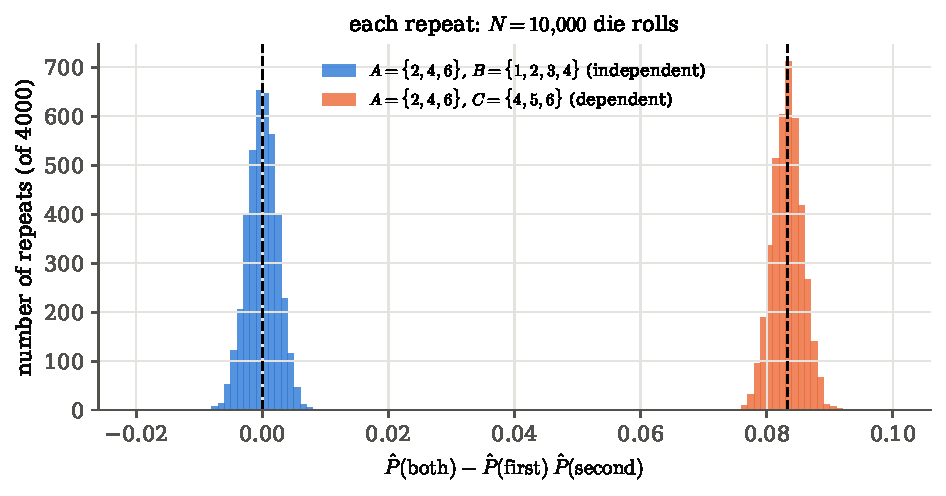
\includegraphics[width=0.85\linewidth]{figures/ch01/1a_independence.pdf}
\caption{The difference between the frequency of ``both'' and the product of the
two frequencies, over many repeats of a $10^4$-roll experiment. For the independent
pair (blue) the differences scatter symmetrically around zero. For the dependent
pair (orange) they scatter around $\tfrac13-\tfrac14=\tfrac1{12}$, far from zero compared with
the width of either histogram.}
\label{1a:fig:indep-hist}
\end{figure}

For the independent pair the differences have mean near zero and standard
deviation $\OneAIndSdAB$. For the dependent pair their mean is $\OneAIndMeanAC$, the
exact $\tfrac1{12}$, some thirty-five standard deviations away. A difference of
$\OneAIndFAB-\OneAIndProdAB$ in the single run is typical of independence. A difference of
$0.08$ is not.

\paragraph{What this bought us.}
With data, ``is $\Prob(AB)=\Prob(A)\Prob(B)$?'' becomes ``is the observed difference
large compared with its scatter under independence?''. That is a hypothesis
test with independence as the null hypothesis, and \cref{ch:04} makes it precise.

\paragraph{In research: independence is what lets us multiply.}
Every likelihood in this book is a product, and every product is an assumption
of independence. Poisson counts in different bins of a histogram are
independent if the events arrive independently (colliders, photon counting). The
spherical-harmonic coefficients $\alm$ of a statistically isotropic Gaussian sky
are independent for different $(\ell,m)$ (\cref{ch:07}), which is why the full-sky
CMB likelihood factorises over $\ell$. For stationary detector noise, the
Fourier amplitudes at different frequencies are independent, which is why the
gravitational-wave log-likelihood is a sum over frequency bins weighted by the
power spectral density (\cref{ch:10}). A mask breaks the $\alm$ independence and
correlated noise breaks the frequency independence. Handling that loss is much
of the work of \cref{ch:08}.

\begin{pitfall}[Three ways to get independence wrong]
(1) Treating disjoint events as independent. (2) Checking only pairs, or only
the full product, for three or more events. (3) Assuming independence where a
hidden common cause exists (a shared power supply, a common calibration
constant, a shared beam condition). Common-mode effects are the usual reason
why a redundant system fails more often than the product of the individual
failure rates predicts.
\end{pitfall}

\section{Bayes' theorem: reading the tree backwards}
\label{1a:sec:bayes}

A tree can be read in two directions, and the analyst at a collider needs the
direction it was not drawn in. Recall the two-level trigger of
\cref{1a:sec:trees}: a fast hardware trigger (L1) followed by a software
high-level trigger (HLT), which together write about one collision in a
hundred to disk. Its tree runs in the order in which things happen. First
nature makes the collision signal ($S$) or background ($B$). Then L1 decides.
Then the HLT decides. Read in that order, the tree answers
\emph{prediction} questions: if a collision is signal, how likely is it to be
kept?

The analyst who opens the files on disk never sees nature's first choice. She
sees only the collisions that were kept. So she asks the opposite question: of
the collisions written to disk, what fraction is signal? That is an
\emph{inference} question. It starts from an observation and asks which branch
of the tree produced it. These are the two directions of probability of
\cref{ch:00}. For a hypothesis $H$ and an observed event $E$, $\Prob(E\given H)$
runs forward, from $H$ to what it produces. $\Prob(H\given E)$ runs backward,
from what we saw to what produced it.

Bayes' theorem turns the first kind of number into the second. We need it
because the two kinds come from different places. The forward numbers are what
physics and calibration give us: efficiencies, misidentification rates,
branching fractions, the probability of the data under a model. The backward
numbers are what we want: the purity of a sample, the probability that a track
is a kaon, the credibility of a cosmological model. So the question is: given a
tree built in the forward direction, how do we read it backwards?

The analyst's question can be said in words, in four steps, before any formula.
\begin{enumerate}[leftmargin=2em,itemsep=1pt]
  \item What did she see? A collision on disk, one that the trigger kept.
  \item What could have put it there? It was either a signal collision or a
        background collision.
  \item If it was signal, how probable was it to be kept? And if it was
        background?
  \item Given those two answers, how must the shares of signal and
        background that nature started with be revised?
\end{enumerate}
Step 3 is ordinary prediction, done once for each hypothesis. Only step 4 is
new, and it needs nothing more than the definition of conditional probability,
used once.

\subsection{Two routes to the same leaf}

The whole theorem rests on one fact: a leaf of a tree is the same event
whichever order the tree was drawn in. Take a hypothesis $H$ and an observed
event $E$. The leaf ``$H$ and $E$'', written $HE$ for $H\cap E$, can be reached
in two orders. In the forward tree we pass first through $H$ and then through
$E$. In a tree drawn the other way round we pass first through $E$ and then
through $H$ \srcref{Lambert}{\S3.6.1}. Both routes end at the same event $HE$, so
they give it the same probability. The multiplication rule \eqref{1a:eq:mult},
$\Prob(HE)=\Prob(E\given H)\Prob(H)$, computes it along the forward route. Dividing
by $\Prob(E)$, which we assume is positive, gives the backward number:
\begin{align}
\Prob(H\given E)
&\eqby{1}\frac{\Prob(HE)}{\Prob(E)}
 \eqby{2}\frac{\Prob(E\given H)\,\Prob(H)}{\Prob(E)} .
\label{1a:eq:bayes-simple}
\end{align}
\begin{explain}
  \item Definition \eqref{1a:eq:cond} of conditional probability, with $E$ as
        the conditioning event: $E$ is the new, shrunk sample space.
  \item Multiplication rule along the forward route,
        $\Prob(HE)=\Prob(E\given H)\Prob(H)$.
\end{explain}
The numerator is one leaf of the forward tree. The denominator $\Prob(E)$ is the
total probability of the observation, and it too comes from the forward tree.
Suppose the possible hypotheses $H_1,\dots,H_k$ form a partition of the sample
space $\Omega$ \unpack{exactly one of them is true}. Then the law of total
probability \eqref{1a:eq:total} gives $\Prob(E)$ as the sum of all the forward
leaves that end in $E$. Putting that sum in the denominator gives the general
form \mainref{p.~12, Thm~1.17}.

\begin{keyidea}[Bayes' theorem]
Let $H_1,\dots,H_k$ be a partition of $\Omega$ with every $\Prob(H_i)>0$, and let
$\Prob(E)>0$. Then for each $i$,
\begin{equation}
\Prob(H_i\given E)
=\frac{\Prob(E\given H_i)\,\Prob(H_i)}{\sum_{j=1}^k\Prob(E\given H_j)\,\Prob(H_j)} .
\label{1a:eq:bayes}
\end{equation}
In the tree: the posterior of $H_i$ is the leaf ``$H_i$ then $E$'' divided by
the sum of all leaves that end in $E$.
\end{keyidea}

Each ingredient has a name \mainref{p.~12, Remark~1.18}.
\begin{itemize}[leftmargin=1.5em,itemsep=1pt]
  \item $\Prob(H_i)$ is the \newterm{prior} probability of $H_i$: how probable
        $H_i$ was before the observation.
  \item $\Prob(H_i\given E)$ is its \newterm{posterior} probability: how probable
        it is after.
  \item $\Prob(E\given H_i)$ is the \newterm{likelihood} of $H_i$: the probability
        of the observation we actually made, computed as if $H_i$ were true.
  \item $\Prob(E)$ is the \newterm{evidence}. It is the same number for every
        $H_i$, and its only job is to make the posteriors add up to one.
\end{itemize}
Nothing here goes beyond the definition of conditional probability and the law
of total probability. The only new thing is the direction in which we read the
tree.

Inverting a tree means: compute the leaves forward, then regroup them by the
observation instead of by the hypothesis. \Cref{1a:fig:invert} shows this for the
trigger. The forward tree and the inverted tree have the same four leaves with
the same probabilities, because the leaves are the same events. What changes is
the order of the two splits, and with it the conditional probabilities written
on the branches.

\begin{figure}[htbp]
\centering
\begin{tikzpicture}[
  nd/.style={font=\small,inner sep=2pt},
  br/.style={thick,accent},
  pr/.style={font=\scriptsize,fill=white,inner sep=1pt},
  lf/.style={font=\scriptsize,anchor=west},
  x=1cm,y=0.8cm]
  \node[font=\small\itshape] at (1.9,2.9) {prediction: nature's order};
  \node[nd] (r) at (0,0) {start};
  \node[nd] (S) at (1.6,1.2) {$S$};
  \node[nd] (B) at (1.6,-1.2) {$B$};
  \node[nd] (SA) at (3.9,1.8) {acc};
  \node[nd] (SR) at (3.9,0.6) {rej};
  \node[nd] (BA) at (3.9,-0.6) {acc};
  \node[nd] (BR) at (3.9,-1.8) {rej};
  \draw[br] (r) -- node[pr,above left] {$0.01$} (S);
  \draw[br] (r) -- node[pr,below left] {$0.99$} (B);
  \draw[br] (S) -- node[pr,above] {$0.855$} (SA);
  \draw[br] (S) -- node[pr,below] {$0.145$} (SR);
  \draw[br] (B) -- node[pr,above] {$0.002$} (BA);
  \draw[br] (B) -- node[pr,below] {$0.998$} (BR);
  \node[lf,fibreorange] at (4.25,1.8) {$0.00855$};
  \node[lf,softgray] at (4.25,0.6) {$0.00145$};
  \node[lf,formblue] at (4.25,-0.6) {$0.00198$};
  \node[lf,softgray!60!black] at (4.25,-1.8) {$0.98802$};
  \begin{scope}[xshift=6.5cm]
  \node[font=\small\itshape] at (1.9,2.9) {inference: observation first};
  \node[nd] (r2) at (0,0) {start};
  \node[nd] (A2) at (1.6,1.2) {acc};
  \node[nd] (R2) at (1.6,-1.2) {rej};
  \node[nd] (AS) at (3.9,1.8) {$S$};
  \node[nd] (AB) at (3.9,0.6) {$B$};
  \node[nd] (RS) at (3.9,-0.6) {$S$};
  \node[nd] (RB) at (3.9,-1.8) {$B$};
  \draw[br] (r2) -- node[pr,above left] {$0.01053$} (A2);
  \draw[br] (r2) -- node[pr,below left] {$0.98947$} (R2);
  \draw[br] (A2) -- node[pr,above] {$0.812$} (AS);
  \draw[br] (A2) -- node[pr,below] {$0.188$} (AB);
  \draw[br] (R2) -- node[pr,above] {$0.0015$} (RS);
  \draw[br] (R2) -- node[pr,below] {$0.9985$} (RB);
  \node[lf,fibreorange] at (4.25,1.8) {$0.00855$};
  \node[lf,formblue] at (4.25,0.6) {$0.00198$};
  \node[lf,softgray] at (4.25,-0.6) {$0.00145$};
  \node[lf,softgray!60!black] at (4.25,-1.8) {$0.98802$};
  \end{scope}
\end{tikzpicture}
\caption{The trigger of \cref{1a:fig:trigger-tree} with the two trigger levels
merged into one decision, accepted (acc) or rejected (rej), drawn in both
orders. Left: nature chooses signal or background, then the trigger decides.
Right: the same four leaves, same colours, same probabilities, regrouped by
the trigger decision first. The branches on the right are the inference
numbers: among accepted collisions, $81\%$ are signal.}
\label{1a:fig:invert}
\end{figure}

\paragraph{Example: inverting the trigger tree.}
\emph{What she saw.} A collision on disk: it passed both L1 and the HLT. Call
this one merged decision ``accepted'', $\mathrm{Acc}=\mathrm{L1}\cap\mathrm{HLT}$.

\emph{What could have produced it?} The collision was either signal, $S$, or
background, $B$. These are the two hypotheses.

\emph{How probable was acceptance under each?} Multiply along the paths of
\cref{1a:fig:trigger-tree}. A signal collision passes L1 with probability
$0.95$ and then the HLT with probability $0.90$, so
$\Prob(\mathrm{Acc}\given S)=0.95\times0.90=0.855$. A background collision passes
L1 with probability $0.02$ and then the HLT with probability $0.10$, so
$\Prob(\mathrm{Acc}\given B)=0.02\times0.10=0.002$.

\emph{Then the priors, and normalise.} Before the trigger, one collision in a
hundred is signal: $\Prob(S)=0.01$, $\Prob(B)=0.99$. The signal fraction of the
recorded sample, called its \newterm{purity}, is
\begin{align*}
\Prob(S\given\mathrm{Acc})
&\eqby{1}\frac{\Prob(\mathrm{Acc}\given S)\,\Prob(S)}
               {\Prob(\mathrm{Acc}\given S)\,\Prob(S)+\Prob(\mathrm{Acc}\given B)\,\Prob(B)}
 \eqby{2}\frac{0.855\times0.01}{0.855\times0.01+0.002\times0.99}\\
&=\frac{0.00855}{0.00855+0.00198}=\frac{0.00855}{0.01053}\approx0.812 .
\end{align*}
\begin{explain}
  \item Bayes' theorem \eqref{1a:eq:bayes} with the partition $\{S,B\}$.
  \item The branch probabilities of the merged tree.
\end{explain}
Only one collision in a hundred is signal, yet four out of five recorded
collisions are. The trigger has raised the probability of ``signal'' from a
prior of $0.01$ to a posterior of $0.81$. The reason is the ratio of the two
likelihoods: a signal collision is $0.855/0.002\approx430$ times more likely to
be accepted than a background one. The simulation of \cref{1a:sec:trees} (the
last line of its listing) counted the signal fraction among the accepted
collisions directly and found $\OneATrigMCPurity$, against the exact
$\OneATrigPurity$.

\paragraph{Example: dots and dashes.}
Morse code sends dots and dashes in the proportion $3:4$, so
$\Prob(\text{dot sent})=\tfrac37$ \srcref{CasellaBerger}{Ex.~1.3.6}. Noise on the line
turns a dot into a dash, or a dash into a dot, with probability $\tfrac18$. We
receive a dot. How sure can we be that a dot was sent?

What we saw is ``dot received''. Two things could have produced it: a dot was
sent and arrived intact, or a dash was sent and noise flipped it. Under the
first, a received dot has probability $\tfrac78$; under the second,
$\tfrac18$. The priors are $\tfrac37$ for a dot and $\tfrac47$ for a dash. Then
\begin{align*}
\Prob(\text{dot sent}\given\text{dot rec.})
\eqby{1}\frac{\tfrac78\cdot\tfrac37}{\tfrac78\cdot\tfrac37+\tfrac18\cdot\tfrac47}
\eqby{2}\frac{21/56}{21/56+4/56}=\frac{21}{25}=0.84 .
\end{align*}
\begin{explain}
  \item Bayes' theorem: the likelihood of ``dot received'' is $\tfrac78$ if a dot
        was sent and $\tfrac18$ if a dash was sent.
  \item Put both products over the common denominator $56$.
\end{explain}
So a received dot is wrong $4$ times in $25$, about one time in six, even though
each symbol is flipped only one time in eight. The extra errors come from the
dashes. Dashes are sent more often than dots, so the flipped dashes make up a
larger share of the received dots than the flip rate alone suggests.

\subsection{The recipe: prior times likelihood, then normalise}

The evidence $\Prob(E)$ is the same for every hypothesis. So we can leave it out,
compute prior times likelihood for each hypothesis, and divide by the total at
the end:
\begin{equation}
\Prob(H_i\given E)\;\propto\;\Prob(E\given H_i)\,\Prob(H_i),
\qquad
\text{then divide by the sum over } i .
\label{1a:eq:bayes-prop}
\end{equation}
This is the most useful form in practice. It turns every discrete Bayes problem
into a table with one row per hypothesis and four columns:
the prior; the likelihood; their product, which is the forward leaf that ends
in $E$; and the product divided by the sum of its column, which is the
posterior. The sum of the product column is $\Prob(E)$.

\paragraph{Example: spam.}
An email is spam ($A_1$), low priority ($A_2$) or high priority ($A_3$), with
prior probabilities $0.7$, $0.2$ and $0.1$ \mainref{pp.~12--13, Ex.~1.19}. The
word ``free'' ($E$) appears in $90\%$ of spam and in $1\%$ of each of the other
two kinds.\footnote{Wasserman prints $\Prob(B\given A_1)=.01$ for the third
likelihood. The subscript should be $A_3$, as the computation that follows it
shows.} An email arrives containing ``free''. That is what we saw, and the three
kinds of email are the hypotheses that could have produced it. The table is
\begin{center}
\small
\begin{tabular}{@{}lcccc@{}}
\toprule
hypothesis & prior $\Prob(A_i)$ & likelihood $\Prob(E\given A_i)$ & product & posterior $\Prob(A_i\given E)$\\
\midrule
spam          & $0.7$ & $0.90$ & $0.630$ & $0.9953$\\
low priority  & $0.2$ & $0.01$ & $0.002$ & $0.0032$\\
high priority & $0.1$ & $0.01$ & $0.001$ & $0.0016$\\
\midrule
sum           & $1$   & $0.92$ & $0.633$ & $1$\\
\bottomrule
\end{tabular}
\end{center}
so $\Prob(A_1\given E)=0.630/0.633\approx0.995$.

The column sums carry a lesson: the likelihoods are not a probability
distribution over the hypotheses. The priors add up to one, and so do the
posteriors, because both are probabilities \emph{over the hypotheses}. The
likelihoods add up to $0.92$, and nothing forces them to add up to one. Each
likelihood is a probability over \emph{outcomes} (does ``free'' appear or not?),
computed in a different world: one where the email is spam, one where it is low
priority, one where it is high priority. Read across those worlds, as a
function of the hypothesis, the list of likelihoods is not a probability
distribution. This is the statement ``$\Prob(A\given\cdot)$ is not a probability''
of \cref{1a:sec:conditional}. It is also why, in \cref{ch:03}, the likelihood of
a parameter is called a function and not a density.

\paragraph{Example: which operating system?}
Among computer owners $30\%$ use a Mac, $50\%$ Windows and $20\%$ Linux, and the
fractions infected by a virus are $0.65$, $0.82$ and $0.50$ \mainref{p.~16,
Ex.~19}. A randomly chosen owner turns out to be infected. The products are
$0.3\times0.65=0.195$, $0.5\times0.82=0.410$ and $0.2\times0.50=0.100$, with sum
$\Prob(\text{infected})=0.705$, so
\begin{align*}
\Prob(\text{Windows}\given\text{infected})=\frac{0.410}{0.705}\approx0.582,\qquad
\Prob(\text{Mac}\given\cdot)\approx0.277,\qquad
\Prob(\text{Linux}\given\cdot)\approx0.142 .
\end{align*}
Windows rises from $0.50$ to $0.58$. Mac falls from $0.30$ to $0.28$, and Linux
from $0.20$ to $0.14$. The rule is visible in the numbers. The average infection
rate is $\Prob(\text{infected})=0.705$. Windows owners are infected more often
than that ($0.82$), so Windows gains. Mac ($0.65$) and Linux ($0.50$) owners are
infected less often, so they lose.

That rule is general: probability can only move between the hypotheses, never
be created or destroyed \mainref{p.~16, Ex.~18}. The reason is that the priors
and the posteriors both add up to one. So if one hypothesis loses, another must
gain. To see it in symbols, suppose $A_1$ loses, $\Prob(A_1\given E)<\Prob(A_1)$.
Then
\begin{align*}
\sum_{i=2}^k\Prob(A_i\given E)\eqby{1}1-\Prob(A_1\given E)\relby{2}{>}1-\Prob(A_1)\eqby{3}\sum_{i=2}^k\Prob(A_i),
\end{align*}
\begin{explain}
  \item $\Prob(\cdot\given E)$ is a probability (\cref{1a:sec:conditional}), and the
        $A_i$ partition $\Omega$, so the posteriors add up to one.
  \item The assumption $\Prob(A_1\given E)<\Prob(A_1)$.
  \item The priors add up to one.
\end{explain}
A sum of $k-1$ terms can be larger than another sum of $k-1$ terms only if at
least one of its terms is larger. So some other hypothesis gains:
$\Prob(A_i\given E)>\Prob(A_i)$ for at least one $i\geq2$. For exactly this reason
Kruschke calls Bayesian inference a \emph{reallocation of credibility} across the
possibilities \srcref{Kruschke}{\S2.1}.

The extreme case is a hypothesis whose likelihood is zero. The observation is
impossible under it, so its posterior is zero. Its prior weight goes to the
hypotheses that survive, shared in proportion to each one's prior times
likelihood. Repeat this with more observations until only one hypothesis is
left, and you get Sherlock Holmes's rule: once every other cause has been ruled
out, the one that remains carries all the probability.

\subsection{Base rates and the odds form}

Bayes' theorem is least intuitive when the prior is small. A test for a rare
disease detects it with probability $\Prob(+\given D)=0.98$, and gives a false
positive with probability $\Prob(+\given D^c)=0.03$. The prevalence is
$\Prob(D)=0.001$ \srcref{Cowan}{p.~4}. You test positive.

\emph{What happened.} The test came back positive, written $+$.
\emph{What could have produced it?} Two situations: you have the disease,
$D$, or you do not, $D^c$. A positive result can come out of either.
\emph{How probable was a positive under each?} With the disease it is the
detection probability, $0.98$; without it, the false-positive rate, $0.03$.
\emph{Then the base rates.} Before the test, $D$ had probability $0.001$ and
$D^c$ had $0.999$. The two forward leaves that end in ``$+$'' give
\begin{align*}
\Prob(D\given +)
\eqby{1}\frac{0.98\times0.001}{0.98\times0.001+0.03\times0.999}
\eqby{2}\frac{0.00098}{0.00098+0.02997}\approx0.032 .
\end{align*}
\begin{explain}
  \item Bayes' theorem \eqref{1a:eq:bayes} with the partition $\{D,D^c\}$.
  \item The two forward leaves that end in ``$+$''.
\end{explain}
The test is wrong only $2\%$ or $3\%$ of the time, yet after a positive result
the probability of disease is only about $3\%$. The two leaves show why. The
false-positive leaf, $0.02997$, is thirty times larger than the true-positive
leaf, $0.00098$. Healthy people rarely test positive, but there are a thousand
times more of them, so they produce most of the positives. The medical test of
\cref{1a:ex:medical}
($\Prob(D\given +)\approx0.08$) and the screening example of
\srcref{Lambert}{\S3.6.2} (also $0.08$) have the same structure. Ignoring the
prior in such a problem is called the \newterm{base-rate fallacy}. It is the
prosecutor's fallacy of \cref{1a:sec:conditional} in another guise: it
confuses $\Prob(+\given D)$ with $\Prob(D\given +)$.

With two hypotheses, the effect of an observation is a single multiplication.
To see it, write Bayes' theorem \eqref{1a:eq:bayes-simple} for $H_1$ and for $H_2$,
and divide one by the other. The evidence $\Prob(E)$ cancels:
\begin{align}
\frac{\Prob(H_1\given E)}{\Prob(H_2\given E)}
&\eqby{1}\frac{\Prob(E\given H_1)\Prob(H_1)/\Prob(E)}{\Prob(E\given H_2)\Prob(H_2)/\Prob(E)}
 \eqby{2}\underbrace{\frac{\Prob(E\given H_1)}{\Prob(E\given H_2)}}_{\text{likelihood ratio}}
 \times\underbrace{\frac{\Prob(H_1)}{\Prob(H_2)}}_{\text{prior odds}} .
\label{1a:eq:odds}
\end{align}
\begin{explain}
  \item Bayes' theorem \eqref{1a:eq:bayes-simple} in the numerator and in the
        denominator.
  \item Cancel $\Prob(E)$ and regroup.
\end{explain}
The ratio on the left is the \newterm{posterior odds}. The observation
multiplies the prior odds by the \newterm{likelihood ratio}, and it does nothing
else. For the rare disease, take $H_1=D$ and $H_2=D^c$. The likelihood ratio is
$0.98/0.03\approx32.7$ and the prior odds are $0.001/0.999\approx0.0010$, so the
posterior odds are $0.0327$. Turning odds back into a probability,
$\Prob(D\given +)=0.0327/(1+0.0327)\approx0.032$, as before. The test is good
evidence (it multiplies the odds by about thirty), but it starts from odds of one
to a thousand.

The odds form makes repeated observations easy: each new observation multiplies
the odds again. Suppose a second test is also positive, and the two results are
independent \emph{given the disease status} (\cref{1a:sec:independence}). Then
yesterday's posterior is today's prior, and the odds are multiplied by $32.7$
again, to $1.07$, so $\Prob(D\given{+}{+})\approx0.52$. A third positive test
gives odds $34.9$ and $\Prob(D\given{+}{+}{+})\approx0.97$. In logarithms the
multiplications become additions: each independent observation \emph{adds} its
log likelihood ratio to the log odds. This is why analyses add up log
likelihoods rather than multiply likelihoods. The condition ``independent given
the disease status'' matters. A test that fails for a reason specific to the
patient will fail again, and then repeating it adds much less
\srcref{Lambert}{Problem~3.8.5}.

\begin{pitfall}[Efficiency is not purity]
A detector's efficiency $\Prob(\text{tag}\given\text{true})$ is a forward number,
measured once on a calibration sample, and it does not depend on what else is
in the beam. The purity $\Prob(\text{true}\given\text{tag})$ is an inverse number, and it
depends strongly on the prior, the composition of the sample. A selection
with $90\%$ efficiency and a $5\%$ fake rate can give a sample that is mostly
fakes, if the true particles are rare. Quote both, and never call one by the
other's name.
\end{pitfall}

\paragraph{Example: particle identification with misidentification.}
A hadron beam contains pions, kaons and protons in the proportions
$0.80:0.15:0.05$. A Cherenkov detector tags a track as ``kaon'' with probability
$0.90$ for a real kaon, $0.05$ for a pion and $0.10$ for a proton. A track is
tagged as a kaon. Which particle is it?

What we saw is the tag ``kaon''. Any of the three species could have produced
it, so they are the three hypotheses. Their priors are the beam proportions,
and their likelihoods are the three tagging probabilities. The table:
\begin{center}
\small
\begin{tabular}{@{}lcccc@{}}
\toprule
species & prior & $\Prob(\text{tag }K\given\text{species})$ & product & posterior\\
\midrule
$\pi$ & $0.80$ & $0.05$ & $0.040$ & $\OneAPidPostPi$\\
$K$   & $0.15$ & $0.90$ & $0.135$ & $\OneAPidPostK$\\
$p$   & $0.05$ & $0.10$ & $0.005$ & $\OneAPidPostP$\\
\midrule
sum   & $1$    &        & $\OneAPidTagK$ & $1$\\
\bottomrule
\end{tabular}
\end{center}
One tagged track in four is not a kaon, and almost all of the impostors are
pions. Pions are misidentified only $5\%$ of the time, but there are more than
five times as many pions as kaons in the beam. So the purity depends on the beam,
not only on the detector. As the kaon fraction falls, the purity collapses
(\cref{1a:fig:pid}). At a kaon fraction of $1\%$ it is only
$\OneAPidPurityOnePct$, with the same detector and the same $90\%$ efficiency.

\begin{figure}[htbp]
\centering
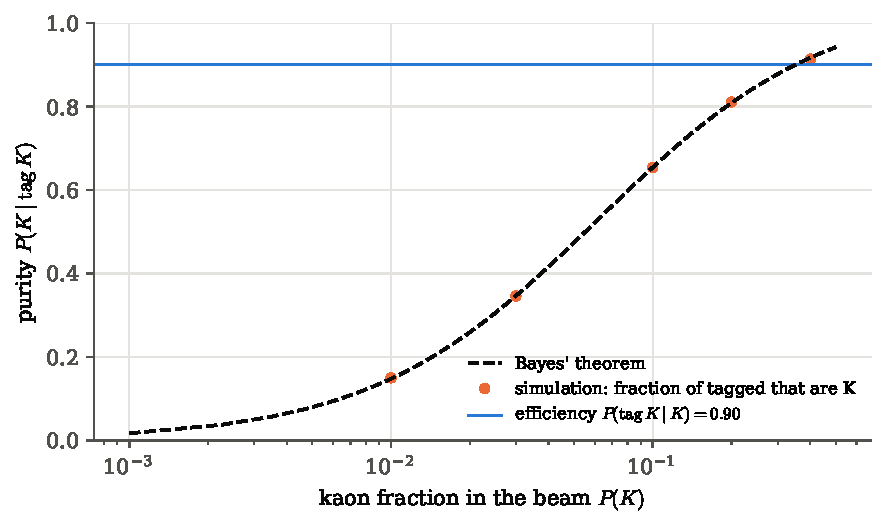
\includegraphics[width=0.75\linewidth]{figures/ch01/1a_particle_id.pdf}
\caption{Purity of the kaon-tagged sample against the kaon fraction of the
beam, on a logarithmic axis. The dashed curve is Bayes' theorem, the dots are
simulated beams in which we tag tracks and count the true kaons among the
tagged ones. The horizontal line is the efficiency, which stays at $0.90$
whatever the beam. The two agree only when kaons dominate.}
\label{1a:fig:pid}
\end{figure}

\subsection{When the observation carries information in how it was produced}

When the observation comes out of a person's choice, intuition tends to ignore
how it was produced, and goes wrong. In the trigger, the detector and the
medical test, the observation came from a fixed mechanism that was easy to see.
In three famous puzzles, Monty Hall, the three prisoners and the three cards,
the mechanism is hidden inside someone's decision.
The four steps of the reasoning handle them without any new idea. Everything
turns on the third step: under each hypothesis, how probable was \emph{exactly
the observation we made}?

\paragraph{Example: Monty Hall.}
A car is behind one of three doors, each with probability $\tfrac13$, and goats
are behind the other two. We pick door 1. The host, Monty, knows where the car
is. He always opens one of the two doors we did not pick, never the car door,
and if he has a choice he picks at random. He opens door 3
\mainref{p.~14, Ex.~10}. Should we switch to door 2?

\emph{What we saw.} Monty opened door 3. Call this event $M_3$.

\emph{What could have made him open it?} Monty's choice depends on one thing
we do not know, where the car is. So the candidate explanations are the
three places the car can be: $H_1$, $H_2$ and $H_3$, the car behind door 1,
2 or 3. We want to know which of these places could have led Monty to open
door 3, and how strongly.

\emph{How likely was door 3 under each location?} Take the three in turn. Monty
knows where the car is, he never reveals it, and he never opens our door.
\begin{itemize}[leftmargin=1.5em,itemsep=1pt]
  \item $H_1$, the car is behind our door 1: both other doors hide goats, so
        Monty can open door 2 or door 3 and chooses at random,
        $\Prob(M_3\given H_1)=\tfrac12$.
  \item $H_2$, the car is behind door 2: he may not open our door 1 and may
        not reveal the car behind door 2, so he is forced to open door 3,
        $\Prob(M_3\given H_2)=1$.
  \item $H_3$, the car is behind door 3: opening door 3 would reveal the car,
        so he cannot open it, $\Prob(M_3\given H_3)=0$.
\end{itemize}
These are the second-stage branches of the tree in \cref{1a:fig:monty-tree}.
\emph{Then the priors, and normalise.} Each location had prior $\Prob(H_d)=\tfrac13$, so
the three leaves that end in $M_3$ weigh $\tfrac13\cdot\tfrac12=\tfrac16$,
$\tfrac13\cdot1=\tfrac13$ and $\tfrac13\cdot0=0$. Normalising by their sum,
\begin{align*}
\Prob(H_2\given M_3)
&\eqby{1}\frac{\Prob(M_3\given H_2)\Prob(H_2)}{\sum_{d=1}^3\Prob(M_3\given H_d)\Prob(H_d)}
 \eqby{2}\frac{1\cdot\tfrac13}{\tfrac12\cdot\tfrac13+1\cdot\tfrac13+0\cdot\tfrac13}
 =\frac{1/3}{1/2}=\frac23,
\end{align*}
\begin{explain}
  \item Bayes' theorem with the partition $\{H_1,H_2,H_3\}$.
  \item The three likelihoods above and the uniform prior. The evidence is
        $\Prob(M_3)=\tfrac16+\tfrac13=\tfrac12$.
\end{explain}
and in the same way $\Prob(H_1\given M_3)=\tfrac16/\tfrac12=\tfrac13$ and
$\Prob(H_3\given M_3)=0$. Switching wins with probability $\tfrac23$.

The whole calculation is one look at the picture of \cref{1a:fig:shrink}, drawn
to scale in \cref{1a:fig:monty-boxes}. The three places the car can be fill the
sample space in three equal strips. The event $M_3$ is a box that takes half of
the $H_1$ strip, all of the $H_2$ strip and none of the $H_3$ strip, exactly the
three likelihoods above. Once we see $M_3$, that box is the whole world, and the
$H_2$ piece of it is twice the $H_1$ piece.

\begin{figure}[htbp]
\centering
\begin{tikzpicture}[scale=0.8]
  \begin{scope}
    \fill[formblue!18] (0,0) rectangle (6,4);
    \fill[tangentgreen!45] (1,0) rectangle (4,4);
    \draw (2,0) -- (2,4); \draw (4,0) -- (4,4);
    \draw[thick] (0,0) rectangle (6,4);
    \draw[line width=1.6pt,fibreorange] (1,0) rectangle (4,4);
    \node[lbl] at (0.5,2) {$H_1$};
    \node[lbl] at (3,3.55) {$H_2$};
    \node[lbl] at (5,2) {$H_3$};
    \node[lbl] at (1.5,1.6) {$\tfrac16$};
    \node[lbl] at (3,1.6) {$\tfrac13$};
    \node[lbl,fibreorange!80!black] at (2.5,4.35) {$M_3$: Monty opens door 3};
    \node[lbl] at (6.25,3.75) {$\Omega$};
    \foreach \a/\b in {0/2,2/4,4/6} {\draw[faint] (\a,-0.15) -- (\a,-0.3) -- (\b,-0.3) -- (\b,-0.15);
      \node[lbl] at ({(\a+\b)/2},-0.6) {$\tfrac13$};}
    \node[lbl,align=center,text width=6.2cm,anchor=north] at (3,-0.95) {before Monty acts: three equal strips,\\ one for each place the car can be};
  \end{scope}
  \draw[->,thick,accent] (6.7,2) -- (8.1,2);
  \node[lbl,accent,align=center] at (7.4,2.75) {observe\\$M_3$};
  \begin{scope}[xshift=8.7cm]
    \draw[faint,dashed] (0,0) rectangle (6,4);
    \draw[faint,dashed] (2,0) -- (2,4); \draw[faint,dashed] (4,0) -- (4,4);
    \fill[tangentgreen!45] (1,0) rectangle (4,4);
    \draw[very thin,black!40] (2,0) -- (2,4);
    \draw[line width=1.6pt,fibreorange] (1,0) rectangle (4,4);
    \node[lbl,align=center] at (1.5,2) {$H_1$\\[2pt]$\tfrac16$};
    \node[lbl,align=center] at (3,2) {$H_2$\\[2pt]$\tfrac13$};
    \node[lbl,softgray,align=center] at (5,2) {$H_3$\\ruled out};
    \node[lbl,fibreorange!80!black] at (2.5,4.35) {$M_3$, area $\tfrac12$};
    \node[lbl,align=center,text width=6.2cm,anchor=north] at (3,-0.95) {after: $M_3$ is the new sample space,\\ $H_2$ fills twice as much of it as $H_1$};
  \end{scope}
\end{tikzpicture}
\caption{Monty Hall drawn to scale in the picture of \cref{1a:fig:shrink}. Left:
the rectangle $\Omega$ has area 1, and since the car is behind exactly one door,
the three hypotheses $H_1$, $H_2$, $H_3$ fill it in three strips of area
$\tfrac13$. The event $M_3$, ``Monty opens door 3'' (orange outline), covers half
of $H_1$ (with the car behind our door he picks door 2 or 3 at random), all of
$H_2$ (he is forced to open door 3) and none of $H_3$ (he never reveals the car),
so its area is $\tfrac16+\tfrac13=\tfrac12$. Right: seeing $M_3$ discards
everything outside the orange box, and each hypothesis keeps the share of the box
that its piece fills: $\tfrac13$ for $H_1$, $\tfrac23$ for $H_2$.}
\label{1a:fig:monty-boxes}
\end{figure}

Most people's first answer is that, with one door gone, the two doors left
must be even. That answer throws away what Monty's choice told us. Door 3 was
not equally likely to be opened under the two locations still possible: with
the car behind door 2, Monty had no other move, while with the car behind our
door 1 he would have opened door 3 only half the time. What we saw is
therefore twice as probable under $H_2$ as under $H_1$, and the posteriors
inherit that factor of two, $\tfrac23$ against $\tfrac13$.

The fifty--fifty answer gets one step right and skips another. It shrinks the
sample space correctly: door 3 is out. But it forgets the likelihoods. A
counterexample shows that they decide the answer. Suppose Monty did \emph{not}
know where the car is, opened door 2 or door 3 at random, and happened to show a
goat behind door 3. Under $H_1$ he opens door 3 with probability $\tfrac12$ and
it hides a goat. Under $H_2$ he also opens door 3 with probability $\tfrac12$,
and it again hides a goat. So
$\Prob(M_3,\text{goat}\given H_1)=\Prob(M_3,\text{goat}\given H_2)=\tfrac12$, and
the answer really would be fifty--fifty. Same doors, same observation, different
mechanism, different posterior.

\begin{figure}[htbp]
\centering
\begin{tikzpicture}[
  nd/.style={font=\small,inner sep=2pt},
  br/.style={thick,accent},
  pr/.style={font=\scriptsize,fill=white,inner sep=1pt},
  lf/.style={font=\small,anchor=west},
  x=1cm,y=0.72cm]
  \node[nd] (r) at (0,0) {car placed};
  \node[nd] (H1) at (2.8,2.6) {$H_1$};
  \node[nd] (H2) at (2.8,0) {$H_2$};
  \node[nd] (H3) at (2.8,-2.6) {$H_3$};
  \node[nd] (a) at (5.6,3.3) {$M_2$};
  \node[nd,fibreorange] (b) at (5.6,1.9) {$M_3$};
  \node[nd,fibreorange] (c) at (5.6,0) {$M_3$};
  \node[nd] (d) at (5.6,-2.6) {$M_2$};
  \draw[br] (r) -- node[pr,above left] {$\tfrac13$} (H1);
  \draw[br] (r) -- node[pr,above] {$\tfrac13$} (H2);
  \draw[br] (r) -- node[pr,below left] {$\tfrac13$} (H3);
  \draw[br] (H1) -- node[pr,above] {$\tfrac12$} (a);
  \draw[br] (H1) -- node[pr,below] {$\tfrac12$} (b);
  \draw[br] (H2) -- node[pr,above] {$1$} (c);
  \draw[br] (H3) -- node[pr,above] {$1$} (d);
  \node[lf,fibreorange] at (6.1,1.9) {$\tfrac16$, posterior $\tfrac{1/6}{1/2}=\tfrac13$};
  \node[lf,fibreorange] at (6.1,0) {$\tfrac13$, posterior $\tfrac{1/3}{1/2}=\tfrac23$};
  \node[lf,softgray] at (6.1,3.3) {$\tfrac16$};
  \node[lf,softgray] at (6.1,-2.6) {$\tfrac13$};
\end{tikzpicture}
\caption{Monty Hall as a tree. We always pick door 1. The first split is where
the car is. The second is which door Monty opens, which is random only when
the car is behind our door. The two orange leaves are the ways of
producing the observation ``Monty opened door 3''. They have probabilities
$\tfrac16$ and $\tfrac13$, and dividing each by their total $\tfrac12$ gives the posterior.
The car cannot be behind door 3, so that hypothesis has no leaf in the
observation.}
\label{1a:fig:monty-tree}
\end{figure}

\paragraph{Example: the three prisoners.}
The same tree appears as an older puzzle \srcref{CasellaBerger}{Ex.~1.3.4}.
One of three prisoners $A$, $B$, $C$ is to be pardoned, each with probability
$\tfrac13$. Prisoner $A$ asks the warden to name one of the \emph{other two} who
will be executed.

\emph{What happened.} The warden names $B$. Call this event $W$.

\emph{What could have made him name $B$?} The one thing $A$ does not know is who
is pardoned, so the hypotheses are ``$A$ pardoned'', ``$B$ pardoned'' and ``$C$
pardoned'', written simply $A$, $B$, $C$. Take them in turn.
\begin{itemize}[leftmargin=1.5em,itemsep=1pt]
  \item If $A$ is pardoned, both $B$ and $C$ will be executed. The warden can name
        either and picks at random, so $\Prob(W\given A)=\tfrac12$.
  \item If $B$ is pardoned, the warden cannot name $B$ as one to be executed, so
        $\Prob(W\given B)=0$.
  \item If $C$ is pardoned, then of $B$ and $C$ only $B$ will be executed, so the
        warden must name $B$: $\Prob(W\given C)=1$.
\end{itemize}
\emph{Then the priors, and normalise.} These are the Monty Hall likelihoods, with
prisoner $A$ in the place of door 1, and the priors are again $\tfrac13$ each. So
$\Prob(A\given W)=\tfrac13$ and $\Prob(C\given W)=\tfrac23$.

Prisoner $A$ reasons ``now it is $A$ or $C$, so my chance has risen to
$\tfrac12$''. He is wrong. The warden is right that he told $A$ nothing about
$A$'s own fate. But he told $A$ a great deal about $C$'s.

\paragraph{Example: three cards.}
One card is green on both sides, one red on both sides, one green on one side
and red on the other. We draw a card at random, look at one side at random,
and see green \mainref{p.~15, Ex.~12}. What is the probability that the other
side is green too?

What we saw is a green face. It could have come from any card that has a green
side, so the hypotheses are the three cards: $GG$, $RR$ and $GR$, with prior
$\tfrac13$ each. Take them in turn. The $GG$ card shows green whichever side we
look at, so the likelihood is $1$. The $RR$ card never shows green: $0$. The $GR$
card shows green only if we happen to look at its green side: $\tfrac12$. The
posterior of $GG$ is
\begin{align*}
\Prob(GG\given\text{see }G)
\eqby{1}\frac{1\cdot\tfrac13}{1\cdot\tfrac13+0\cdot\tfrac13+\tfrac12\cdot\tfrac13}
\eqby{2}\frac{1/3}{1/2}=\frac23,
\end{align*}
\begin{explain}
  \item Bayes' theorem with the partition $\{GG,RR,GR\}$.
  \item The evidence is $\Prob(\text{see }G)=\tfrac12$, as it must be by symmetry
        between the colours.
\end{explain}
and the hidden side is green exactly when the card is $GG$. The popular answer,
$\tfrac12$, counts cards: two cards have a green side, so it treats them as
equally likely. But what we saw was a face, not a card. The correct answer
counts green \emph{faces}. There are three, and two of them are on the $GG$
card.

\subsection{A posterior over a parameter: coins in a box}

The hypotheses can be the possible values of a number, not just named
situations. Then the posterior is a probability distribution over that number.
That is the step from the puzzles to parameter estimation.

\paragraph{Example: which coin?}
A bag holds a fair coin and a biased coin with $\Prob(\text{heads})=0.95$. We pick
one at random and toss it three times, getting three heads, $H_3$
\srcref{SeeingTheory}{pp.~28--29}. Which coin did we pick? The hypotheses are
``biased'' and ``fair'', each with prior $\tfrac12$. Given the coin, the tosses
are independent, so the likelihoods of three heads are $0.95^3=0.857$ for the
biased coin and $0.5^3=0.125$ for the fair one. In \cref{1a:ex:bag-total} we
computed the two forward leaves,
$\Prob(H_3\given\text{biased})\Prob(\text{biased})=0.857\times0.5$ and
$\Prob(H_3\given\text{fair})\Prob(\text{fair})=0.125\times0.5$, and their sum
$\Prob(H_3)\approx0.491$. Reading that tree backwards,
\begin{align*}
\Prob(\text{biased}\given H_3)=\frac{0.857\times0.5}{0.491}\approx0.873 .
\end{align*}
Three heads move the biased coin from $\tfrac12$ to $0.87$. In the odds form
\eqref{1a:eq:odds}: the prior odds were $1$, the likelihood ratio is
$0.857/0.125\approx6.9$, so the posterior odds are $6.9$.

\paragraph{Example: five coins, and a prediction from a posterior.}
A box holds five coins whose probabilities of heads are $p_1=0$, $p_2=\tfrac14$,
$p_3=\tfrac12$, $p_4=\tfrac34$ and $p_5=1$ \mainref{p.~16, Ex.~20}. We pick coin $C_i$ at
random, prior $\tfrac15$ each, toss it once and get heads ($H_1$). The likelihood of
coin $i$ is $p_i$, so
\begin{align*}
\Prob(C_i\given H_1)
\eqby{1}\frac{p_i\cdot\tfrac15}{\sum_jp_j\cdot\tfrac15}
\eqby{2}\frac{p_i}{5/2}
=\bigl(0,\;0.1,\;0.2,\;0.3,\;0.4\bigr)\quad\text{for } i=1,\dots,5 .
\end{align*}
\begin{explain}
  \item Bayes' theorem. The uniform prior cancels between numerator and
        denominator.
  \item $\sum_jp_j=0+\tfrac14+\tfrac12+\tfrac34+1=\tfrac52$.
\end{explain}
With a flat prior, the posterior is just the likelihood, rescaled to add up to
one. The two-headed coin ($p_5=1$) is now the most probable, and the two-tailed
coin ($p_1=0$) is ruled out.

Now toss the same coin again. What is the probability of another head,
$\Prob(H_2\given H_1)$, where $H_2$ is ``heads on the second toss''? We do not
know which coin we hold, so we average over the coins. Given the coin $C_i$,
the tosses are independent, so $\Prob(H_2\given C_iH_1)=p_i$. The conditional
probability $\Prob(\cdot\given H_1)$ is itself a probability
(\cref{1a:sec:conditional}), so every rule holds for it, including the law of
total probability. Hence
\begin{align*}
\Prob(H_2\given H_1)
&\eqby{1}\sum_{i=1}^5\Prob(H_2\given C_iH_1)\,\Prob(C_i\given H_1)
 \eqby{2}\sum_{i=1}^5p_i\,\Prob(C_i\given H_1)\\
&\eqby{3}\frac{\sum_ip_i^2}{\sum_ip_i}
 =\frac{0+\tfrac1{16}+\tfrac14+\tfrac9{16}+1}{5/2}=\frac{15/8}{5/2}=\frac34 .
\end{align*}
\begin{explain}
  \item Law of total probability \eqref{1a:eq:total} for the probability
        $\Prob(\cdot\given H_1)$, over the partition $\{C_i\}$. Each term is
        $\Prob(H_2C_i\given H_1)=\Prob(H_2\given C_iH_1)\Prob(C_i\given H_1)$ by the
        multiplication rule applied inside $\Prob(\cdot\given H_1)$.
  \item Given the coin, the second toss does not care about the first.
  \item The posterior from the previous chain.
\end{explain}
The chance of heads has gone from $\tfrac12$ to $\tfrac34$. Before any toss, it
was the prior average of $p_i$, which is $\tfrac12$. After one head it is the
\emph{posterior} average of $p_i$, which is $\tfrac34$. This is a
\newterm{posterior predictive} probability: a prediction made by averaging over
what we still do not know, weighted by what we now believe. So the two tosses
are \emph{not} independent: $\Prob(H_2\given H_1)=\tfrac34\neq\Prob(H_2)=\tfrac12$.
They are independent only given the coin. The first head changes the forecast
for the second because it tells us something about the coin.

Finally, suppose instead that we toss the chosen coin until the first head,
and it arrives on toss 4 ($B_4$). The likelihood of coin $i$ is three tails and
then a head, $(1-p_i)^3p_i$:
\begin{align*}
\bigl((1-p_i)^3p_i\bigr)_{i=1}^5&=\Bigl(0,\;\tfrac{27}{256},\;\tfrac{16}{256},\;\tfrac{3}{256},\;0\Bigr),\\
\Prob(C_i\given B_4)&=\Bigl(0,\;\tfrac{27}{46},\;\tfrac{16}{46},\;\tfrac{3}{46},\;0\Bigr)
\approx(0,\;0.59,\;0.35,\;0.07,\;0),
\end{align*}
where the second list is the first divided by its sum $\tfrac{46}{256}$ (the flat
prior again cancels). A late first head favours a coin with a small $p$. Both
extreme coins are eliminated: $p_1=0$ never gives a head, and $p_5=1$ gives one
on the first toss.

The five values $p_i$ are a coarse grid over a continuous parameter, the
probability of heads $p\in[0,1]$. With a finer and finer grid, the posterior
becomes a density $p(p\given\data)$, where $\data$ stands for the observed
tosses, and the sum in the evidence becomes an integral. That is the subject of
\cref{ch:05}.

\subsection{Bayes' theorem in a simulation: selecting on the observation}

Bayes' theorem can be simulated in one line, because conditioning is selection
(\cref{1a:sec:conditional}). The recipe has three steps.
\begin{enumerate}[leftmargin=2em,itemsep=1pt]
  \item Generate many trials in the forward order, exactly as the tree says:
        first the hypothesis, then the observation.
  \item Keep only the trials in which the observation came out as it actually
        did.
  \item Among those, count how often each hypothesis was the true one.
\end{enumerate}
That fraction estimates the posterior, and no formula is involved. Here it is
for the particle-identification beam of the kaon-tagging example.

\pyfile[firstline=30,lastline=35,firstnumber=30]{code/ch01/07_particle_id_bayes.py}{Bayes' theorem by selecting tagged tracks}

Line 33 is the first split of the tree, the true species of each of a million
tracks, drawn from the beam composition (the prior). Line 34 is the second
split, the detector's decision. \texttt{p\_tag[true]} looks up, for each track,
the tagging probability of its own species, so this line uses exactly the
likelihoods of the table. Line 35 is the inversion: \texttt{true[tagged]} keeps
the true species of the tagged tracks only, and \texttt{np.bincount} counts how
many are pions, kaons and protons. Of the $\OneAPidNtag$ tagged tracks, the
fractions are $\OneAPidMCPi$, $\OneAPidMCK$ and $\OneAPidMCP$, against the exact
posteriors $\OneAPidPostPi$, $\OneAPidPostK$ and $\OneAPidPostP$. The same selection,
repeated for five beam compositions, gives the dots in \cref{1a:fig:pid}.

For Monty Hall the forward simulation must also contain Monty's rule, because
his rule is the likelihood.

\pyfile[firstline=26,lastline=32,firstnumber=26]{code/ch01/08_monty_hall.py}{Monty Hall by selecting the games in which door 3 was opened}

Line 26 places the prize (the prior). Lines 29--30 are Monty's behaviour, which
is the likelihood: with the prize behind door 1 he opens door 2 or 3 according
to a fair coin, otherwise he opens the one empty door we did not pick. Line 31
selects the observation, ``Monty opened door 3'', which happened in
$\OneAMontyNsel$ of the $\OneAMontyN$ games, a fraction $\OneAMontyOpenThree$
(exact $\tfrac12$, the evidence). Line 32 counts where the prize was in those
games: door 1 in a fraction $\OneAMontyPostOne$, door 2 in $\OneAMontyPostTwo$,
door 3 in $\OneAMontyPostThree$. Over all games, switching won
$\OneAMontySwitch$ of the time and staying $\OneAMontyStay$
(\cref{1a:fig:monty}). The three-card problem is simulated the same way in the
same script: of the $\OneACardsNgreen$ draws that showed a green face, the
hidden face was green in a fraction $\OneACardsHiddenGreen$ (exact $\tfrac23$).

\begin{figure}[htbp]
\centering
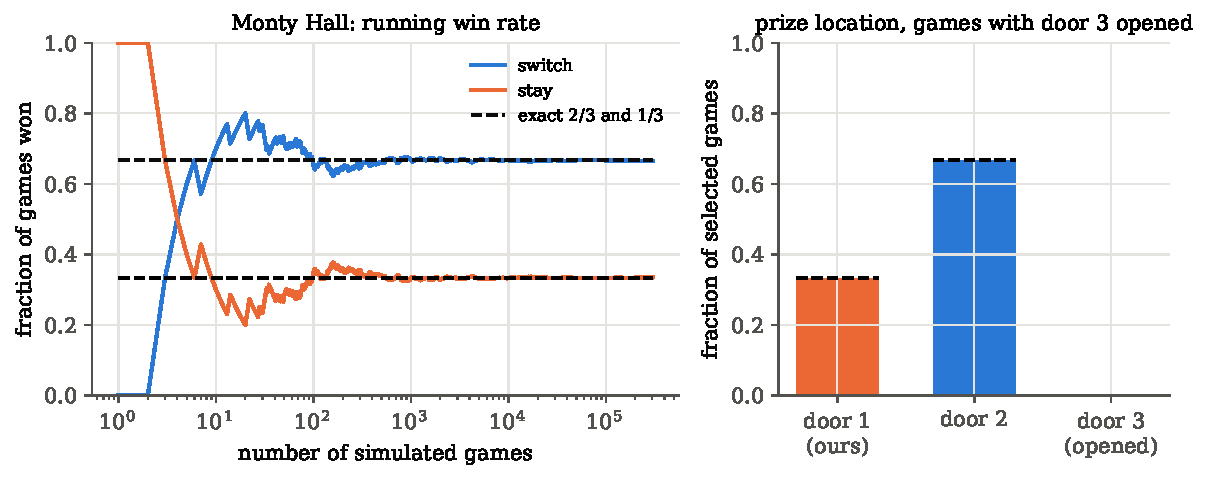
\includegraphics[width=0.95\linewidth]{figures/ch01/1a_monty_hall.pdf}
\caption{Monty Hall by simulation. Left: the running fraction of games won by
always switching and by always staying, settling on $\tfrac23$ and $\tfrac13$.
Right: among the games in which Monty opened door 3, where the prize was. The
bars are the posterior, estimated by counting, and the dashed ticks are the
exact values $\tfrac13$ and $\tfrac23$.}
\label{1a:fig:monty}
\end{figure}

\begin{inpractice}[Selecting on the observation is how analyses estimate purity]
Here the simulation only verified a posterior that Bayes' theorem gives in
one line. In a real analysis the ``hypotheses'' are the physics processes
(signal and every background), the ``observation'' is a long list of
selection cuts, and the likelihood of passing them depends on the kinematics
of each event, for which no formula exists. The expected composition of the
selected sample is then computed exactly as above: simulate each process with
its cross section as the prior weight, apply the selection, and count what
survives. The numbers that come out are the prior-times-likelihood column of
the table, event by event, and the fractions among the survivors are the
posterior. Bayes' theorem in its tabular form is also how particle-ID
systems combine the responses of several detectors: the likelihood ratios of
independent subdetectors multiply, as in \eqref{1a:eq:odds}, and the prior is
the expected particle mix.
\end{inpractice}

\subsection{Where this goes}

Every later chapter uses one of the two directions, prediction or inference,
and many use both. Side by side:
\begin{center}
\small
\begin{tabular}{@{}p{0.44\linewidth}p{0.44\linewidth}@{}}
\toprule
prediction & inference\\
\midrule
start from a hypothesis $H$ & start from an observed event $E$\\
ask what outcomes it can produce & ask which hypotheses could have produced it\\
uses $\Prob(E\given H)$, the forward tree & wants $\Prob(H\given E)$, the tree read backwards\\
efficiency, sampling distribution, $p$-value & purity, posterior, credible interval\\
\bottomrule
\end{tabular}
\end{center}
They are not rival interpretations of probability. They are two questions
about one joint probability structure, the leaves of a single tree.

From the trigger to the five coins, every example was settled by two sentences
said before any symbol. First: which hypotheses could have given what we saw?
They are the rows of the table, and the posterior is spread over them. Second:
how probable was the observation under each one? That is the likelihood
column. \Cref{ch:05} turns this into a standing habit.

The arithmetic is always the same, but the meaning of the posterior depends on
the hypotheses. When they are outcomes of a repeatable process (signal or
background, which coin, which door), a posterior is a long-run frequency among
the selected trials, as the simulations showed. When the hypothesis is a value
of a physical constant, which nature chose once, there are no repeated trials
to count. Then the posterior can only be read as a degree of belief, the second
interpretation of \cref{1a:sec:axioms}.

In the pipeline that runs from a physical model, through the data and a summary
of them, to physics inferred, the forward tree is the sampling distribution
$P(S\given\theta)$ of a summary $S$ computed from the data, given the model
parameters $\theta$. Reading that tree backwards is the last arrow, inference. \Cref{ch:05} replaces the list of hypotheses by a continuous
parameter $\params$, the likelihood by $\Like(\params)=p(\data\given\params)$ (the
probability density of the data $\data$ given $\params$), and the sum in the
evidence by the integral $Z=p(\data)=\int p(\data\given\params)\,p(\params)\,\dd\params$,
which runs over every possible parameter value and is usually the hard part.
\Cref{ch:09} avoids computing it at all: in the proportional form
\eqref{1a:eq:bayes-prop} only ratios of posteriors appear, and $Z$ cancels in
every ratio, just as $\Prob(E)$ cancelled in the odds \eqref{1a:eq:odds}. In
\cref{ch:04} we meet the forward direction on its own, in the $p$-value, which
is a statement about $\Prob(\text{data}\given\Hnull)$, the probability of the data
if the null hypothesis $\Hnull$ (``nothing but chance'') were true. It must
never be read as $\Prob(\Hnull\given\text{data})$.

\subsection*{Reading the literature}
\begin{description}[leftmargin=1.5em,itemsep=2pt]
  \item[Events.] \mainref{pp.~3--5, \S1.2} Wasserman defines $\Omega$, outcomes and events in three lines and gives the
three examples of \cref{1a:ex:aos-spaces}, the table of terminology
(our dictionary, where $\varnothing$ is the ``null event'' that is always false
and $\Omega$ the ``true event''), disjointness, partitions, indicators and the
limits of monotone sequences with the example $[0,1/i)$. He writes $A\cap B$ as
$AB$ or $(A,B)$, the convention used from here on. The proofs of De Morgan's
laws and the distributive law are exercises there (\mainref{p.~14, Ex.~4}) and
worked in \srcref{SeeingTheory}{pp.~20--21}. Kruschke adds the point that the
sample space is set by the measurement operation \srcref{Kruschke}{\S4.1}.
  \item[Axioms.] \mainref{pp.~5--7, 13, \S1.3, \S1.9} Wasserman states the axioms (Definition 1.5, footnote on $\sigma$-fields), the
two interpretations in one paragraph, the properties (1.1) without proof,
inclusion--exclusion (Lemma 1.6) with the proof we expanded, the two-toss
example (Example 1.7) and continuity (Theorem 1.8, increasing case only, the
decreasing case being his Exercise~1). The appendix \S1.9 defines $\sigma$-fields,
probability spaces and the Borel $\sigma$-field. Cowan \srcref{Cowan}{\S1.1} lists
finite additivity instead of countable additivity as the third axiom, noting
that this is a simplification. Countable additivity is what makes continuity
and \cref{1a:ex:no-uniform-N} work. The Bonferroni inequality and the
disjointification in Boole's inequality are from \srcref{CasellaBerger}{\S1.2};
the electron-mass argument is \srcref{Cowan}{\S1.2.2}; calibration by gambles is
\srcref{Kruschke}{\S4.2.2}.
  \item[Counting.] \mainref{pp.~7--8, \S1.4} Wasserman treats finite sample spaces in a page: the $36$ outcomes of two dice,
$\Prob(\text{sum}=11)=2/36$, the uniform distribution $\Prob(A)=|A|/|\Omega|$,
$n!$ with $0!=1$, the binomial coefficient (1.2), the committee of $3$ from $20$
($1140$), and $\binom n0=\binom nn=1$, $\binom nk=\binom n{n-k}$. He writes that
``we needn't delve into these in any great detail'', which is why we supplied
the derivations. The two-by-two table of counting rules, stars and bars, the
lottery and poker counts, and the warning that unordered outcomes with
replacement are not equally likely come from \srcref{CasellaBerger}{\S1.2.3--1.2.4}.
The recursion $P_n=nP_{n-1}$ and counting by overcounting are from
\srcref{SeeingTheory}{pp.~22--24}. The birthday problem is not treated in these sources.
  \item[Trees.] \mainref{p.~12, Thm~1.16} Wasserman states the law of total probability for a finite partition and
proves it in one line, as in our chain. He draws no trees. The tree picture,
with the first stage as the hypotheses and the second as the outcomes they
produce, organises the librarian--farmer, Monty Hall and medical-test problems above, and Lambert's ``two routes to the joint probability''
\srcref{Lambert}{\S3.6.1} is a two-stage tree read in both orders. Cowan
derives the same law as (1.7) \srcref{Cowan}{p.~3}, and Seeing Theory's
coins in a bag is \cref{1a:ex:bag-total} \srcref{SeeingTheory}{pp.~28--29}.
  \item[Independence.] \mainref{pp.~8--10, \S1.5} Wasserman defines independence by the product rule (Definition 1.9, with
$A\amalg B$ for independence), distinguishes assumed from derived independence
with the die events $\{2,4,6\}$ and $\{1,2,3,4\}$, shows that disjoint events with
positive probability are dependent and that a Venn diagram cannot display
independence, and gives Examples 1.10 and 1.11 and a summary box. His
Exercises 11, 14, 15 and 23 are solved above. The pairwise and mutual examples
and de M\'er\'e's bet are from \srcref{CasellaBerger}{\S1.3}, the card-colour and
causation remarks from \srcref{Lambert}{\S3.4}, and suit versus value from
\srcref{Kruschke}{\S4.4.2}. Seeing Theory lists $B=\{\text{second flip heads}\}$ as
$\{HT,TT\}$ \srcref{SeeingTheory}{p.~12}. It should be $\{HH,TH\}$.
  \item[Conditioning and Bayes.] Conditional probability and Bayes' theorem are \mainref{pp.~11--13, \S1.6--1.7}, \srcref{Cowan}{\S1.2}, \srcref{CasellaBerger}{\S1.3}, \srcref{Kruschke}{\S4.4} and \srcref{SeeingTheory}{pp.~26--30}.
Wasserman gives the law of total probability and Bayes' theorem as Theorems 1.16
and 1.17 \mainref{pp.~12--17}, the names prior and posterior in Remark 1.18, the
spam example as Example 1.19, and Monty Hall, the three cards, the rule that a
losing hypothesis forces another to gain, the operating systems and the five
coins as Exercises 10, 12, 18, 19 and 20. The two routes to
the joint probability are \srcref{Lambert}{\S3.6}. The disease example and the
combined form of the theorem are \srcref{Cowan}{pp.~3--4, (1.6)--(1.8)}. The
Morse-code and prisoners examples are \srcref{CasellaBerger}{\S1.3}, and the
coins in a bag are \srcref{SeeingTheory}{pp.~28--29}.
\end{description}

\begin{recap}[Events, conditional probability and trees]
\begin{itemize}[leftmargin=1.2em,itemsep=1pt]
  \item An experiment has a sample space $\Omega$ of outcomes. Events are subsets,
        combined by $\cup$, $\cap$ and complement. In code an event is a Boolean
        mask over simulated outcomes.
  \item Probability obeys three axioms. Complement rule, monotonicity,
        inclusion--exclusion, Boole's inequality and continuity all follow.
        It can be read as a long-run frequency or as a degree of belief.
  \item With equally likely outcomes, probability is counting:
        $\Prob(A)=|A|/|\Omega|$, with $n!$ and $\binom nk$ as the tools (birthday problem).
  \item Information shrinks the sample space: $\Prob(A\given B)=\Prob(AB)/\Prob(B)$,
        the overlap re-measured against the surviving region $B$. In code,
        \texttt{A[B].mean()}.
  \item Trees: multiply along a path (chain rule), add across paths (law of
        total probability, a weighted average over the unobserved stage).
  \item Independence, $\Prob(AB)=\Prob(A)\Prob(B)$, is not disjointness. Mutual
        independence needs every sub-collection.
  \item Bayes' theorem reads the tree backwards:
        $\Prob(H_i\given E)\propto\Prob(E\given H_i)\Prob(H_i)$, normalised by
        $\Prob(E)=\sum_j\Prob(E\given H_j)\Prob(H_j)$. Posterior odds are the
        likelihood ratio times the prior odds.
  \item Efficiency is a forward number, purity an inverse one. Small priors
        make even good evidence weak (base rates).
\end{itemize}
\end{recap}
\providecommand{\oneBEx}[1]{\par\medskip\noindent\refstepcounter{wex}\textbf{Example~\thewex\ifx\relax#1\relax\else\ (#1)\fi.}\ }
\providecommand{\OneBBernP}{}\renewcommand{\OneBBernP}{0.3}
\providecommand{\OneBBernFrac}{}\renewcommand{\OneBBernFrac}{0.3016}
\providecommand{\OneBNOmega}{}\renewcommand{\OneBNOmega}{10^5}
\providecommand{\OneBNExp}{}\renewcommand{\OneBNExp}{2\times10^{5}}
\providecommand{\OneBMeanX}{}\renewcommand{\OneBMeanX}{4.997}
\providecommand{\OneBMeanY}{}\renewcommand{\OneBMeanY}{2.796}
\providecommand{\OneBPXfive}{}\renewcommand{\OneBPXfive}{0.2467}
\providecommand{\OneBPXfiveExact}{}\renewcommand{\OneBPXfiveExact}{0.2461}
\providecommand{\OneBPYthree}{}\renewcommand{\OneBPYthree}{0.2606}
\providecommand{\OneBPeakExact}{}\renewcommand{\OneBPeakExact}{1.596}
\providecommand{\OneBPeakEst}{}\renewcommand{\OneBPeakEst}{1.612}
\providecommand{\OneBFracOneSig}{}\renewcommand{\OneBFracOneSig}{0.683}
\providecommand{\OneBQoneSample}{}\renewcommand{\OneBQoneSample}{49.826}
\providecommand{\OneBQoneExact}{}\renewcommand{\OneBQoneExact}{49.831}
\providecommand{\OneBMedSample}{}\renewcommand{\OneBMedSample}{49.996}
\providecommand{\OneBMedExact}{}\renewcommand{\OneBMedExact}{50.000}
\providecommand{\OneBQthreeSample}{}\renewcommand{\OneBQthreeSample}{50.146}
\providecommand{\OneBQthreeExact}{}\renewcommand{\OneBQthreeExact}{50.169}
\providecommand{\OneBMargN}{}\renewcommand{\OneBMargN}{2\times10^{5}}
\providecommand{\OneBMargSdY}{}\renewcommand{\OneBMargSdY}{2.006}
\providecommand{\OneBMargSdX}{}\renewcommand{\OneBMargSdX}{1.001}
\providecommand{\OneBBandN}{}\renewcommand{\OneBBandN}{4855}
\providecommand{\OneBCondMeanSim}{}\renewcommand{\OneBCondMeanSim}{1.404}
\providecommand{\OneBCondMeanExact}{}\renewcommand{\OneBCondMeanExact}{1.400}
\providecommand{\OneBCondSdSim}{}\renewcommand{\OneBCondSdSim}{1.426}
\providecommand{\OneBCondSdExact}{}\renewcommand{\OneBCondSdExact}{1.428}
\providecommand{\OneBSmearN}{}\renewcommand{\OneBSmearN}{5\times10^{5}}
\providecommand{\OneBSmearMeanSim}{}\renewcommand{\OneBSmearMeanSim}{19.99}
\providecommand{\OneBSmearVarSim}{}\renewcommand{\OneBSmearVarSim}{425.0}
\providecommand{\OneBSmearVarExact}{}\renewcommand{\OneBSmearVarExact}{425.0}
\providecommand{\OneBSmearNegSim}{}\renewcommand{\OneBSmearNegSim}{0.0866}
\providecommand{\OneBSmearNegExact}{}\renewcommand{\OneBSmearNegExact}{0.0860}
\providecommand{\OneBSmearChi}{}\renewcommand{\OneBSmearChi}{125}
\providecommand{\OneBSmearNdf}{}\renewcommand{\OneBSmearNdf}{136}
\providecommand{\OneBOscN}{}\renewcommand{\OneBOscN}{2\times10^{5}}
\providecommand{\OneBOscFracSim}{}\renewcommand{\OneBOscFracSim}{0.2872}
\providecommand{\OneBOscFracExact}{}\renewcommand{\OneBOscFracExact}{0.2871}
\providecommand{\OneBOscChi}{}\renewcommand{\OneBOscChi}{65.4}
\providecommand{\OneBOscNbins}{}\renewcommand{\OneBOscNbins}{60}
\providecommand{\OneBOscMeanSq}{}\renewcommand{\OneBOscMeanSq}{0.4995}
\providecommand{\OneBRuleChi}{}\renewcommand{\OneBRuleChi}{54.7}
\providecommand{\OneBRuleNbins}{}\renewcommand{\OneBRuleNbins}{50}
\providecommand{\OneBRuleFracSim}{}\renewcommand{\OneBRuleFracSim}{0.0478}
\providecommand{\OneBRuleFracExact}{}\renewcommand{\OneBRuleFracExact}{0.0477}
\providecommand{\OneBDecN}{}\renewcommand{\OneBDecN}{4\times10^{5}}
\providecommand{\OneBDecPstar}{}\renewcommand{\OneBDecPstar}{40.2}
\providecommand{\OneBDecMeanPtSim}{}\renewcommand{\OneBDecMeanPtSim}{31.566}
\providecommand{\OneBDecMeanPtExact}{}\renewcommand{\OneBDecMeanPtExact}{31.573}
\providecommand{\OneBDecFracSim}{}\renewcommand{\OneBDecFracSim}{0.4353}
\providecommand{\OneBDecFracExact}{}\renewcommand{\OneBDecFracExact}{0.4359}
\providecommand{\OneBDecMeanCos}{}\renewcommand{\OneBDecMeanCos}{0.0006}
\providecommand{\OneBExpUSim}{}\renewcommand{\OneBExpUSim}{1.7189}
\providecommand{\OneBExpUExact}{}\renewcommand{\OneBExpUExact}{1.7183}
\providecommand{\OneBStickSim}{}\renewcommand{\OneBStickSim}{0.7498}
\providecommand{\OneBHierMean}{}\renewcommand{\OneBHierMean}{9.997}
\providecommand{\OneBHierVar}{}\renewcommand{\OneBHierVar}{36.67}
\providecommand{\OneBHierVarExact}{}\renewcommand{\OneBHierVarExact}{36.67}
\providecommand{\OneBPlainVar}{}\renewcommand{\OneBPlainVar}{4.998}
\providecommand{\OneBArgminSq}{}\renewcommand{\OneBArgminSq}{1.00}
\providecommand{\OneBArgminAbs}{}\renewcommand{\OneBArgminAbs}{0.69}
\providecommand{\OneBMinSq}{}\renewcommand{\OneBMinSq}{0.996}
\providecommand{\OneBGalRa}{}\renewcommand{\OneBGalRa}{-0.795}
\providecommand{\OneBGalRb}{}\renewcommand{\OneBGalRb}{0.040}
\providecommand{\OneBGalRc}{}\renewcommand{\OneBGalRc}{0.486}
\providecommand{\OneBGalRd}{}\renewcommand{\OneBGalRd}{0.949}
\providecommand{\OneBZeroRxy}{}\renewcommand{\OneBZeroRxy}{0.0046}
\providecommand{\OneBZeroRxxy}{}\renewcommand{\OneBZeroRxxy}{1.0000}
\providecommand{\OneBZeroRabsxy}{}\renewcommand{\OneBZeroRabsxy}{0.9359}
\providecommand{\OneBZeroN}{}\renewcommand{\OneBZeroN}{2\times10^{5}}
\providecommand{\OneBCovN}{}\renewcommand{\OneBCovN}{2\times10^{5}}
\providecommand{\OneBChataa}{}\renewcommand{\OneBChataa}{3.998}
\providecommand{\OneBChatab}{}\renewcommand{\OneBChatab}{1.798}
\providecommand{\OneBChatbb}{}\renewcommand{\OneBChatbb}{0.999}
\providecommand{\OneBCYaa}{}\renewcommand{\OneBCYaa}{8.595}
\providecommand{\OneBCYab}{}\renewcommand{\OneBCYab}{2.999}
\providecommand{\OneBCYbb}{}\renewcommand{\OneBCYbb}{1.401}
\providecommand{\OneBCWaa}{}\renewcommand{\OneBCWaa}{0.157}
\providecommand{\OneBCWab}{}\renewcommand{\OneBCWab}{-0.001}
\providecommand{\OneBCWbb}{}\renewcommand{\OneBCWbb}{4.840}
\providecommand{\OneBLamA}{}\renewcommand{\OneBLamA}{0.157}
\providecommand{\OneBLamB}{}\renewcommand{\OneBLamB}{4.843}
\providecommand{\OneBLaa}{}\renewcommand{\OneBLaa}{2.000}
\providecommand{\OneBLba}{}\renewcommand{\OneBLba}{0.900}
\providecommand{\OneBLbb}{}\renewcommand{\OneBLbb}{0.436}
\providecommand{\OneBMgfMone}{}\renewcommand{\OneBMgfMone}{0.9993}
\providecommand{\OneBMgfMtwo}{}\renewcommand{\OneBMgfMtwo}{1.9993}
\providecommand{\OneBCfMaxDev}{}\renewcommand{\OneBCfMaxDev}{0.0073}
\providecommand{\OneBCfInvDev}{}\renewcommand{\OneBCfInvDev}{0.0004}
\providecommand{\OneBCfN}{}\renewcommand{\OneBCfN}{10^5}
\providecommand{\OneBRunGaussMax}{}\renewcommand{\OneBRunGaussMax}{0.022}
\providecommand{\OneBRunCauchyMin}{}\renewcommand{\OneBRunCauchyMin}{0.28}
\providecommand{\OneBRunCauchyMax}{}\renewcommand{\OneBRunCauchyMax}{1.21}
\providecommand{\OneBRunN}{}\renewcommand{\OneBRunN}{10^4}
\section{Random variables: turning outcomes into numbers}
\label{1b:sec:rv}

A charged track crosses ten layers of a silicon tracker. Each layer either
records a hit or misses it. The raw outcome of one track is therefore a
10-letter pattern such as \texttt{HHTHHTHHTT} (H for hit, T for miss). Nobody
analyses patterns directly. The track-quality cut asks for a \emph{number}:
``how many hits?'' A pattern-recognition algorithm asks for a different
number: ``what is the longest run of consecutive hits?'' Both numbers are
computed from the same pattern, and both are uncertain before the track
arrives.

A \newterm{random variable} is exactly this: a rule that reads a number off
each outcome. We want numbers because a pattern of letters cannot be put in a
histogram, averaged or added, and a number can. Every data point, every
estimator and every summary statistic in the rest of the book is a random
variable.

Recall the box $\Omega$ of all possible outcomes from the first part of
\cref{ch:01}, where the probability of an event was its share of the area of
the box. A random variable is a measuring device clipped onto that box.
Nature picks the point $\omega$, and the device prints the number
$X(\omega)$. Nothing random happens inside the device. It is an ordinary
function, and all the randomness is in which $\omega$ nature picked. Several
devices can be clipped onto the same box, and each reads its own number off
the \emph{same} outcome. This is why two random variables can be related to
each other (correlated, dependent): both are functions of one common
$\omega$.

Building a random variable takes four questions, asked in this order.
\begin{enumerate}[leftmargin=1.5em,itemsep=1pt]
  \item What is one outcome $\omega$? (One full hit pattern, one collision
        event record, one sky map.)
  \item What number do we want to read off it? Write it as a rule
        $\omega\mapsto X(\omega)$.
  \item For each set $A$ of numbers we might ask about, which outcomes give a
        value in $A$? That set of outcomes is an event, and its probability is
        the probability that $X$ lands in $A$.
  \item Collect those probabilities for all $A$. That list is the
        \emph{distribution} of $X$, and from then on we can mostly forget
        $\Omega$.
\end{enumerate}

\subsection{The definition, and the event hiding behind every statement about \texorpdfstring{$X$}{X}}

The four questions give one definition. They also give a rule we will use
constantly: every statement about the number $X$ is a statement about a set
of outcomes.

\begin{workdef}[random variable, distribution]
A \newterm{random variable} is a map
\[
  X:\Omega\to\R
\]
that assigns a real number $X(\omega)$ to each outcome $\omega$
\unpack{a fixed rule, such as ``count the H's'', applied to whichever
outcome occurs}. For a set $A\subseteq\R$ the \newterm{inverse image} is
$X^{-1}(A)=\{\omega\in\Omega:\ X(\omega)\in A\}$ \unpack{all outcomes whose
reading lands in $A$. It is a set of outcomes, not an inverse function}, and
\[
  \Prob(X\in A)\;\defeq\;\Prob\bigl(X^{-1}(A)\bigr),\qquad
  \Prob(X=x)\;\defeq\;\Prob\bigl(\{\omega:\ X(\omega)=x\}\bigr).
\]
The collection of all the numbers $\Prob(X\in A)$ is the
\newterm{distribution} of $X$ \unpack{how the probability of $\Omega$ is
spread along the real line by the map $X$}.
\emph{Operational test:} you have a random variable when, given any outcome,
you can compute a single real number from it without further information.
\end{workdef}

Capital $X$ is the random variable (the rule). Lower-case $x$ is a particular
value it can take. ``$X=x$'' is therefore an event: the set of outcomes whose
reading is $x$. (Strictly, $X$ must be \newterm{measurable}: every set
$\{\omega:X(\omega)\le x\}$ must be an event we are allowed to assign a
probability to. Every function met in practice is, and we will not mention it
again \mainref{p.~43}.)

\begin{figure}[htbp]
\centering
\begin{tikzpicture}[scale=1.0,
  pt/.style={circle,fill=formblue,inner sep=1.4pt},
  val/.style={circle,fill=fibreorange,inner sep=1.6pt}]
  \draw[thick,formblue,fill=formblue!8] plot[smooth cycle,tension=0.8]
    coordinates {(-0.2,0.2) (1.6,1.6) (3.4,1.1) (3.6,-0.9) (1.8,-1.7) (0.1,-1.1)};
  \node[lbl,formblue] at (0.2,1.35) {$\Omega$};
  \node[pt] (tt) at (1.2,-0.9) {}; \node[lbl,anchor=east] at (1.1,-0.9) {TT};
  \node[pt] (th) at (2.0,0.9) {};  \node[lbl,anchor=north] at (2.0,0.8) {TH};
  \node[pt] (ht) at (2.3,-0.3) {}; \node[lbl,anchor=north] at (2.3,-0.4) {HT};
  \node[pt] (hh) at (0.9,0.6) {};  \node[lbl,anchor=east] at (0.8,0.6) {HH};
  \draw[->,thick] (6.0,-1.8) -- (6.0,2.0) node[above,lbl] {$\R$};
  \foreach \y/\t in {-1/0, 0.2/1, 1.4/2} {
    \draw (5.9,\y) -- (6.1,\y);
    \node[lbl,anchor=west] at (6.15,\y) {$\t$};
  }
  \node[val] (v0) at (6.0,-1) {};
  \node[val] (v1) at (6.0,0.2) {};
  \node[val] (v2) at (6.0,1.4) {};
  \draw[->,faint,thick,shorten >=2pt] (tt) to[out=10,in=190] (v0);
  \draw[->,faint,thick,shorten >=2pt] (th) to[out=0,in=175] (v1);
  \draw[->,faint,thick,shorten >=2pt] (ht) to[out=10,in=185] (v1);
  \draw[->,faint,thick,shorten >=2pt] (hh) to[out=40,in=180] (v2);
  \node[lbl,align=left,anchor=west] at (7.0,1.4) {$X^{-1}(\{2\})=\{\mathrm{HH}\}$};
  \node[lbl,align=left,anchor=west] at (7.0,0.2) {$X^{-1}(\{1\})=\{\mathrm{TH},\mathrm{HT}\}$};
  \node[lbl,align=left,anchor=west] at (7.0,-1.0) {$X^{-1}(\{0\})=\{\mathrm{TT}\}$};
\end{tikzpicture}
\caption{A random variable is a function from outcomes to numbers. For two
coin flips, $X$ = number of heads sends the four outcomes to three numbers.
Two outcomes land on the value 1, so the probability that $X=1$ collects the
probability of both. The inverse images on the right are the events that
statements about $X$ secretly refer to.}
\label{1b:fig:rv-map}
\end{figure}

\oneBEx{Two flips: from the outcome table to the distribution}\label{1b:ex:two-flips}
Flip a fair coin twice, $\Omega=\{\mathrm{TT},\mathrm{TH},\mathrm{HT},\mathrm{HH}\}$,
each outcome with probability $1/4$, and let $X$ be the number of heads. Then
\begin{align*}
  \Prob(X=1)
  &\eqby{1} \Prob\bigl(\{\omega:\ X(\omega)=1\}\bigr)\\
  &\eqby{2} \Prob\bigl(\{\mathrm{TH},\mathrm{HT}\}\bigr)\\
  &\eqby{3} \Prob(\{\mathrm{TH}\})+\Prob(\{\mathrm{HT}\})
   = \tfrac14+\tfrac14=\tfrac12 .
\end{align*}
\begin{explain}
  \item Definition of $\Prob(X=x)$ as the probability of the inverse image.
  \item Read off which outcomes contain exactly one H.
  \item The two outcomes are disjoint events, so the axiom of additivity
        (first part of \cref{ch:01}) adds their probabilities.
\end{explain}
In the same way $\Prob(X=0)=\Prob(\{\mathrm{TT}\})=1/4$ and
$\Prob(X=2)=\Prob(\{\mathrm{HH}\})=1/4$. Two tables summarise the situation:
\begin{center}
\begin{tabular}{c|c|c}
$\omega$ & $\Prob(\{\omega\})$ & $X(\omega)$\\\hline
TT & 1/4 & 0\\ TH & 1/4 & 1\\ HT & 1/4 & 1\\ HH & 1/4 & 2
\end{tabular}
\qquad\qquad
\begin{tabular}{c|c}
$x$ & $\Prob(X=x)$\\\hline
0 & 1/4\\ 1 & 1/2\\ 2 & 1/4
\end{tabular}
\end{center}
The left table describes the outcomes themselves. The right table is the
distribution of $X$, and it answers every question about $X$ alone. What the
right table has lost, \emph{which} flip was the head, is exactly what $X$
does not measure.

\oneBEx{Several random variables on one disk}\label{1b:ex:disk}
Pick a point uniformly at random in the unit disk
$\Omega=\{(x,y):\ x^2+y^2\le1\}$, so that the probability of a region is its
area divided by $\pi$. The outcome is the point $\omega=(x,y)$. Four random
variables on the same $\Omega$ are $X(\omega)=x$, $Y(\omega)=y$,
$Z(\omega)=x+y$ and $W(\omega)=\sqrt{x^2+y^2}$ \mainref{p.~20}. Let us find the
distribution of the distance $W$ from the centre. For $0\le r\le1$,
\begin{align*}
  \Prob(W\le r)
  &\eqby{1} \Prob\bigl(\{(x,y):\ x^2+y^2\le r^2\}\bigr)\\
  &\eqby{2} \frac{\pi r^2}{\pi}
   = r^2 .
\end{align*}
\begin{explain}
  \item $W\le r$ happens exactly for the points inside the circle of radius $r$.
  \item Uniform on the disk means probability = area$/\pi$, and the small disk
        has area $\pi r^2$.
\end{explain}
So $\Prob(W\le\tfrac12)=\tfrac14$: a ``uniformly random point'' is \emph{not}
uniformly distributed in its distance from the centre. Three quarters of the
area lies in the outer ring $\tfrac12<W\le1$. A detector that is uniformly
illuminated sees most hits near its rim, simply because the rim has more area.

\subsection{Bernoulli and binomial: one trial and many trials}

The simplest random variables take only two values. Many of the most useful
ones in the book are sums of them.

\begin{workdef}[Bernoulli and binomial]
$X$ is \newterm{Bernoulli}$(p)$ if $\Prob(X=1)=p$ and $\Prob(X=0)=1-p$
\unpack{a single yes-or-no trial, 1 for success}. Compactly
$\Prob(X=x)=p^x(1-p)^{1-x}$ for $x\in\{0,1\}$.
$X$ is \newterm{binomial}$(n,p)$ if it counts the successes in $n$
successive, independent Bernoulli$(p)$ trials \unpack{the same trial repeated
$n$ times, with outcomes that do not influence each other}.
\emph{Operational test:} a single detector layer that fires or not is
Bernoulli. The number of the ten layers that fired is binomial, provided the
layers have the same efficiency and fire independently.
\end{workdef}

Bernoulli is for a single trial; binomial is for multiple successive trials.
That is the whole difference between the two. A binomial variable is a sum of Bernoulli variables,
$X=X_1+\dots+X_n$ with $X_i$ the indicator of success on trial $i$.

\oneBEx{The binomial distribution, by counting paths}\label{1b:ex:binomial}
Generalise \cref{1b:ex:two-flips} to $n$ trials with success probability
$p$ \mainref{p.~20 (``try generalizing this to $n$ flips'')}. An outcome is
a sequence of $n$ letters. Consider one particular sequence with exactly $k$
successes, say $\mathrm{S}^k\mathrm{F}^{n-k}$ (all successes first). Then
\begin{align*}
  \Prob(\mathrm{S}\cdots\mathrm{S}\,\mathrm{F}\cdots\mathrm{F})
  &\eqby{1} \underbrace{p\cdots p}_{k}\;\underbrace{(1-p)\cdots(1-p)}_{n-k}
   = p^k(1-p)^{n-k},\\
  \Prob(X=k)
  &\eqby{2} \sum_{\text{sequences with $k$ S}} p^k(1-p)^{n-k}
   \eqby{3} \binom{n}{k}p^k(1-p)^{n-k},\qquad k=0,1,\dots,n .
\end{align*}
\begin{explain}
  \item The trials are independent, so the probability of a sequence is the
        product of the probabilities of its letters.
  \item $\{X=k\}$ is the disjoint union of all sequences with exactly $k$
        successes, and every one of them has the same probability (only the
        number of S's matters, not their positions).
  \item The number of such sequences is the number of ways to choose which
        $k$ of the $n$ positions carry an S, $\binom{n}{k}=n!/(k!(n-k)!)$
        (the counting rule of the first part of \cref{ch:01}).
\end{explain}
For $n=10$, $p=\tfrac12$: $\Prob(X=5)=\binom{10}{5}/2^{10}=252/1024=0.2461$.
Simulated coin tosses give $\OneBPXfive$, against the exact
$\OneBPXfiveExact$. The binomial and its relatives (geometric, Poisson,
multinomial) are derived from first principles in \cref{ch:02}.

\oneBEx{The sample space that ``disappears''}\label{1b:ex:bern-construction}
The named distributions are usually stated with no $\Omega$ in sight. Is
there still a set of outcomes behind them? Yes: one can always be built
\mainref{p.~27}. Take $\Omega=[0,1]$ with
$\Prob([a,b])=b-a$ (uniform), fix $p$, and define
\[
  X(\omega)=\begin{cases}1,&\omega\le p,\\ 0,&\omega>p.\end{cases}
\]
Then
\begin{align*}
  \Prob(X=1)
  &\eqby{1} \Prob(\{\omega:\ \omega\le p\})
   \eqby{2} \Prob([0,p])
   \eqby{3} p ,
\end{align*}
\begin{explain}
  \item Inverse image of the value 1 under the rule above.
  \item The outcomes with $\omega\le p$ form the interval $[0,p]$.
  \item Uniform probability of an interval is its length.
\end{explain}
and $\Prob(X=0)=1-p$, so $X\sim\text{Bernoulli}(p)$. This is not a
curiosity: it is exactly how a computer makes a Bernoulli variable,
\texttt{x = (u <= p)} with \texttt{u} a uniform random number
(\cref{ch:06} makes this the general recipe). In practice we think of a random
variable as ``a random number''. Formally it is still a function on some
$\Omega$.

\begin{pitfall}[Three notational traps]
\begin{itemize}[leftmargin=1.2em,itemsep=1pt]
  \item $X\sim F$ means ``$X$ \emph{has} distribution $F$'', not ``$X$ is
        approximately $F$'' \mainref{p.~25}.
  \item In Binomial$(n,p)$, $X$ is random and $x$ is a value it can take,
        but $n$ and $p$ are \newterm{parameters}: fixed numbers of the model.
        The parameter is usually unknown and has to be learned from data.
        That is what statistical inference is about. Do not confuse the
        random variable with the parameter \mainref{p.~26}.
  \item $X$ and $Y$ are \newterm{equal in distribution}, $X\overset{d}{=}Y$,
        if $\Prob(X\le x)=\Prob(Y\le x)$ for every $x$. This does not mean
        $X=Y$. If $\Prob(X=1)=\Prob(X=-1)=\tfrac12$ and $Y=-X$, then $X$ and $Y$
        have the same distribution but $\Prob(X=Y)=0$ \mainref{p.~25}.
\end{itemize}
\end{pitfall}

\subsection{Seeing it: two random variables on the same outcomes}

A simulation shows two random variables read off the same outcomes. The
script first builds a Bernoulli variable from a uniform $\omega$, as in
\cref{1b:ex:bern-construction}. It then generates $\OneBNExp$ outcomes of ten fair flips (each row of an array is one
$\omega$) and applies two different maps to every row: $X$ = number of heads
and $Y$ = longest run of heads.

\pyfile[firstline=25,lastline=50,firstnumber=25]{code/ch01/10_rv_as_map.py}{Two random variables read off the same simulated outcomes}

Lines 26--29 are \cref{1b:ex:bern-construction} verbatim: \texttt{omega} is
an array of $\OneBNOmega$ uniform outcomes and \texttt{X\_bern} is the boolean
test $\omega\le p$ turned into 0/1. Its average is the fraction of ones,
$\OneBBernFrac$ for $p=\OneBBernP$. Line 33 draws the outcomes of the second
experiment: an array with one row per outcome and one column per flip. The two
maps on lines 44--45 are ordinary Python functions of a row, which is the
definition of a random variable made executable. Lines 47--50 estimate each
distribution by the fraction of outcomes that land on each value.

\begin{figure}[htbp]
\centering
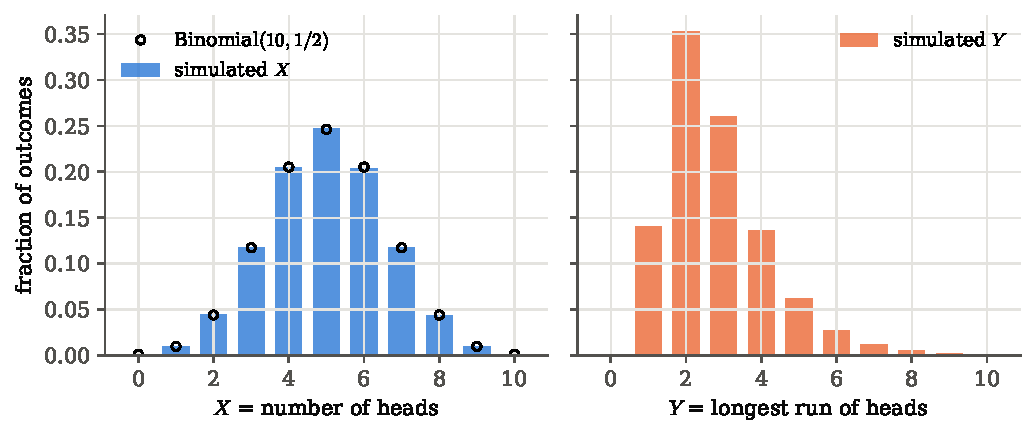
\includegraphics[width=0.95\linewidth]{figures/ch01/rv_as_map.pdf}
\caption{The same $2\times10^5$ simulated ten-flip outcomes, read by two
different random variables. Left: the number of heads, whose fractions sit on
the binomial probabilities (open circles). Right: the longest run of heads,
which has a completely different, skewed distribution although it is computed
from exactly the same outcomes.}
\label{1b:fig:rv-as-map}
\end{figure}

The numbers the script produced: the simulated $\Prob(X=5)$ is
$\OneBPXfive$ (exact $\OneBPXfiveExact$), the average number of heads is
$\OneBMeanX$ (we will show in \cref{1b:sec:expectation} that the exact value
is $np=5$), the average longest run is $\OneBMeanY$, and the most likely
longest run is 2, with $\Prob(Y=3)=\OneBPYthree$. No simple formula gives the
distribution of $Y$. The simulation gets it with the same effort as the
binomial one, because once we can generate outcomes, \emph{any} random
variable is just a function applied to them.

\paragraph{What this bought us.} A random variable is a function, so a
histogram of a random variable is a histogram of a function evaluated on
simulated outcomes. That single sentence is the whole of Monte Carlo
simulation (\cref{ch:06}).

\paragraph{How research uses it.} A collider Monte Carlo generator produces
outcomes $\omega$: complete event records with every particle's
four-momentum. An analysis then defines random variables on them: the missing
transverse momentum, the invariant mass of the two leading jets, the number of
$b$-tagged jets. The same $\omega$'s feed every observable, which is why one
simulated sample serves a whole collaboration, and why two observables
computed from the same events are in general correlated
(\cref{1b:sec:covariance}). In cosmology the outcome is a whole simulated sky
map, and the random variables are its summaries: a power spectrum $\Chat$ at
each $\ell$, the number of hot spots above a threshold, the Euler
characteristic of an excursion set (\cref{ch:07,ch:12}).

Later chapters use many named random variables. The table lists the named
distributions of \mainref{pp.~26--30}, each with the mechanism that produces
it. \Cref{ch:02}
derives every one of them from its mechanism.

\begin{taxonomy}[Named random variables and the story that produces each]
\begin{center}
\small
\begin{tabular}{@{}p{3.2cm}p{9.2cm}@{}}
\toprule
distribution & generating story\\\midrule
point mass $\delta_a$ & no randomness at all, $\Prob(X=a)=1$\\
discrete uniform & $k$ equally likely labels (a fair die)\\
Bernoulli$(p)$ & one yes/no trial\\
Binomial$(n,p)$ & successes in $n$ independent identical trials\\
Geometric$(p)$ & number of trials up to and including the first success, $p(1-p)^{k-1}$\\
Poisson$(\lambda)$ & counts of rare events in a fixed window (decays, events in a bin), $e^{-\lambda}\lambda^k/k!$\\
Uniform$(a,b)$ & ``a point at random'' in an interval, density $1/(b-a)$\\
Normal $\Normal(\mu,\sigma^2)$ & sums of many small independent effects (noise)\\
Exponential$(\beta)$ & waiting time to the next rare event, density $e^{-x/\beta}/\beta$\\
Gamma, $\chi^2_p$, $t_\nu$, Beta, Cauchy & sums of waiting times, sums of squared Gaussians, ratios, probabilities of probabilities, resonance line shapes\\
\bottomrule
\end{tabular}
\end{center}
\end{taxonomy}

\section{Mass, density and the cumulative distribution}
\label{1b:sec:pdf}

A test beam fires electrons of exactly $50\,\mathrm{GeV}$ into an
electromagnetic calorimeter. The calorimeter does not report 50 every time:
the shower fluctuates and the readout is noisy, so the measured energy $E$
scatters around 50 with a spread of about $0.25\,\mathrm{GeV}$. We want to
answer questions such as ``what fraction of electrons are measured below
49.5?'', ``which energy is exceeded by only 5\% of them?'' and ``how does the
histogram of measured energies look if we take more data?''

Three objects describe how a random variable is spread out: the probability
mass function for counts, the density for continuous readings, and the
cumulative distribution for both. We need more than one because counts and
continuous readings differ in kind. For a count (hits, heads) we can list the
probability of each value. For a continuous reading like $E$ we cannot,
because the probability of measuring \emph{exactly} $50.000\ldots$ is zero.
Each of the three objects can be read off a histogram. The idea people get
wrong most often is that a density is probability \emph{per unit} $x$, so it
carries units.

Mass and density are familiar from mechanics. A string of beads has point masses. A metal rod has a mass density
$\lambda(x)$ in kg/m, and the mass of a piece is $\int\lambda\,\dd x$. Nobody
asks ``what is the mass at the point $x=0.3\,$m?''. The answer is zero, and
yet $\lambda(0.3)$ is a perfectly good number. Probability works the same
way. Discrete random variables are beads: the probability sits on isolated
values. Continuous random variables are rods: the probability of a single
point is zero, and $f(x)$ is probability per unit length. The cumulative
distribution $F(x)$ is ``the mass to the left of $x$'', which makes sense for
beads, rods and anything in between.

To describe how a random number is spread out, we ask four questions in turn.
\begin{enumerate}[leftmargin=1.5em,itemsep=1pt]
  \item Does $X$ take isolated values (counts) or a continuum (energies,
        angles, positions)?
  \item Isolated values: list $\Prob(X=x)$ for each value.
  \item Continuum: ask instead for the probability of a small interval,
        divided by its width. That ratio is the density.
  \item Either way: the probability of landing at or below $x$ is a single
        function $F(x)$ that answers every interval question by subtraction,
        and whose inverse gives the quantiles.
\end{enumerate}

\subsection{The cumulative distribution function}

Beads and rods need different bookkeeping, but one function works for both:
the total probability collected up to a point.

\begin{workdef}[cumulative distribution function]
The \newterm{cumulative distribution function} (CDF) of $X$ is
\[
  F_X(x)=\Prob(X\le x),\qquad x\in\R ,
\]
\unpack{the probability that the reading is at most $x$, defined for every
real $x$, including values $X$ never takes}. We write $F$ when the variable is
clear.
\emph{Operational test:} sort a sample of $N$ readings. The fraction of
readings $\le x$ is the \newterm{empirical CDF}, and it tends to $F(x)$ as
$N\to\infty$.
\end{workdef}

\oneBEx{The CDF of two flips}\label{1b:ex:cdf-two-flips}
With $X$ = number of heads in two fair flips (\cref{1b:ex:two-flips}),
\[
  F_X(x)=\begin{cases}
  0, & x<0,\\ 1/4, & 0\le x<1,\\ 3/4, & 1\le x<2,\\ 1, & x\ge2 .
  \end{cases}
\]
For instance
\begin{align*}
  F_X(1.4)
  &\eqby{1} \Prob(X\le1.4)
   \eqby{2} \Prob(X=0)+\Prob(X=1)
   = \tfrac14+\tfrac12=\tfrac34 .
\end{align*}
\begin{explain}
  \item Definition of the CDF at the point $x=1.4$.
  \item $X$ only takes the values 0, 1, 2, and the ones $\le1.4$ are 0 and 1.
        The events $\{X=0\}$ and $\{X=1\}$ are disjoint, so their
        probabilities add.
\end{explain}
The CDF is a staircase. It is flat between the values, jumps by
$\Prob(X=x)$ at each value, and at a jump takes the \emph{upper} value (the
filled dots in \cref{1b:fig:cdf-steps}): $F(1)=3/4$, not $1/4$, because
$X\le1$ includes $X=1$.

\begin{figure}[htbp]
\centering
\begin{tikzpicture}[x=1.2cm,y=2.4cm]
  \begin{scope}
    \draw[->] (-0.6,0) -- (2.8,0) node[right,lbl] {$x$};
    \draw[->] (-0.6,0) -- (-0.6,1.15) node[above,lbl] {$\Prob(X=x)$};
    \foreach \y in {0.25,0.5,0.75,1} {\draw (-0.65,\y) -- (-0.55,\y);
      \node[lbl,anchor=east] at (-0.65,\y) {\y};}
    \foreach \x in {0,1,2} \node[lbl,anchor=north] at (\x,0) {\x};
    \draw[very thick,formblue] (0,0) -- (0,0.25);
    \draw[very thick,formblue] (1,0) -- (1,0.5);
    \draw[very thick,formblue] (2,0) -- (2,0.25);
    \fill[formblue] (0,0.25) circle (2pt) (1,0.5) circle (2pt) (2,0.25) circle (2pt);
    \node[lbl] at (1.1,1.1) {mass function};
  \end{scope}
  \begin{scope}[xshift=5.2cm]
    \draw[->] (-0.9,0) -- (2.9,0) node[right,lbl] {$x$};
    \draw[->] (-0.6,0) -- (-0.6,1.15) node[above,lbl] {$F_X(x)$};
    \foreach \y in {0.25,0.5,0.75,1} {\draw (-0.65,\y) -- (-0.55,\y);
      \node[lbl,anchor=east] at (-0.65,\y) {\y};}
    \foreach \x in {0,1,2} \node[lbl,anchor=north] at (\x,0) {\x};
    \draw[very thick,formblue] (-0.9,0) -- (0,0);
    \draw[very thick,formblue] (0,0.25) -- (1,0.25);
    \draw[very thick,formblue] (1,0.75) -- (2,0.75);
    \draw[very thick,formblue] (2,1) -- (2.8,1);
    \draw[faint,dashed] (0,0) -- (0,0.25) (1,0.25) -- (1,0.75) (2,0.75) -- (2,1);
    \fill[formblue] (0,0.25) circle (2pt) (1,0.75) circle (2pt) (2,1) circle (2pt);
    \filldraw[fill=white,draw=formblue,thick] (0,0) circle (2pt) (1,0.25) circle (2pt) (2,0.75) circle (2pt);
    \draw[bdryred,thick,dotted] (1.4,0) -- (1.4,0.75);
    \node[lbl,bdryred,anchor=north] at (1.4,-0.12) {$1.4$};
    \node[lbl] at (1.0,1.1) {CDF};
  \end{scope}
\end{tikzpicture}
\caption{Two fair flips. Left: the mass function puts probability $1/4$,
$1/2$, $1/4$ on the values 0, 1, 2. Right: the CDF accumulates it into a
staircase that jumps by those amounts. Filled dots mark the value the CDF
takes at each jump, open dots the value it approaches from the left. The
dotted line reads off $F(1.4)=3/4$.}
\label{1b:fig:cdf-steps}
\end{figure}

Every CDF has three properties, and conversely any function with these
properties is the CDF of some random variable \mainref{Thm~2.8, p.~21}:
\begin{enumerate}[label=(\roman*),leftmargin=2em,itemsep=1pt]
  \item \emph{non-decreasing}: $x_1<x_2\Rightarrow F(x_1)\le F(x_2)$, because
        $\{X\le x_1\}\subseteq\{X\le x_2\}$;
  \item \emph{normalised}: $F(x)\to0$ as $x\to-\infty$ and $F(x)\to1$ as
        $x\to+\infty$;
  \item \emph{right-continuous}: $F(x)=\lim_{y\downarrow x}F(y)$.
\end{enumerate}
Property (iii) is why the CDF takes the upper value at each jump (the filled
dots). Why does it hold? The tool is the \emph{continuity of probability}
from the first part of \cref{ch:01}: if
$A_1\supseteq A_2\supseteq\cdots$ shrink to $A=\bigcap_iA_i$, then
$\Prob(A)=\lim_i\Prob(A_i)$. Take any sequence $y_1>y_2>\cdots$ decreasing to
$x$, and $A_i=\{X\le y_i\}$. Then
\begin{align*}
  F(x)
  &\eqby{1} \Prob(X\le x)
   \eqby{2} \Prob\Bigl(\bigcap_i\{X\le y_i\}\Bigr)
   \eqby{3} \lim_i\Prob(X\le y_i)
   = \lim_i F(y_i) .
\end{align*}
\begin{explain}
  \item Definition of $F$.
  \item $X\le x$ holds exactly when $X\le y_i$ for every $i$, because the
        $y_i$ come arbitrarily close to $x$ from above.
  \item The events $\{X\le y_i\}$ shrink, so continuity of probability applies.
\end{explain}
From the left the argument fails. The events $\{X\le y_i\}$ with $y_i\uparrow
x$ grow to $\{X<x\}$, and that event misses the point $X=x$. This asymmetry
gives the handy rules of \mainref{Lemma~2.15, pp.~24--25}. Write
$F(x^-)=\lim_{y\uparrow x}F(y)$. Then
\begin{align}
  \Prob(X=x)&=F(x)-F(x^-), &
  \Prob(x<X\le y)&=F(y)-F(x), &
  \Prob(X>x)&=1-F(x). \label{1b:eq:cdf-rules}
\end{align}
The first says that the size of the jump at $x$ is the probability of the
value $x$. The second is additivity: $\{X\le y\}$ is the disjoint union of
$\{X\le x\}$ and $\{x<X\le y\}$. The third is the complement rule.

\subsection{Discrete variables: the probability mass function}

For counts the bookkeeping is the simplest one, a list of probabilities, one
per allowed value.

\begin{workdef}[probability mass function]
$X$ is \newterm{discrete} if it takes countably many values $x_1,x_2,\dots$
\unpack{values that can be listed one after another, like $0,1,2,\dots$}. Its
\newterm{probability mass function} (pmf) is $f_X(x)=\Prob(X=x)$. It
satisfies $f_X(x)\ge0$, $\sum_if_X(x_i)=1$, and
$F_X(x)=\sum_{x_i\le x}f_X(x_i)$.
\emph{Operational test:} from $N$ simulated or measured values, the fraction
equal to $x_i$ estimates $f_X(x_i)$. The fractions are pure numbers and none
can exceed 1.
\end{workdef}

A set is countable if its elements can be listed so that each one is reached
after finitely many steps. The integers are countable: list them as
$0,1,-1,2,-2,\dots$. The real numbers in $[0,1]$ are not. Cantor's diagonal argument builds, from any proposed list, a number
that differs from the $n$-th entry in its $n$-th decimal, so it is missing
from the list \srcref{SeeingTheory}{pp.~33--34}. A Poisson count can take
infinitely many values and is still discrete.

\subsection{Continuous variables: density is probability per unit \texorpdfstring{$x$}{x}}

Return to the calorimeter of the opening, which measures $50\,\mathrm{GeV}$
electrons with a spread of about $0.25\,\mathrm{GeV}$. Divide the energy axis
into bins of width $\Delta$, record $N$ electrons and let $n_i$ be the number
in bin $i$. The fraction $n_i/N$ estimates the probability of the bin. It
depends on the bin width: halve $\Delta$ and every fraction roughly halves.
Dividing by the width removes this dependence. The ratio
\[
  \frac{n_i}{N\,\Delta}
  \;\approx\;\frac{\Prob(\text{bin } i)}{\Delta}
\]
does \emph{not} depend on the bin width once the bins are narrow, and as
$N\to\infty$ and $\Delta\to0$ it becomes a smooth function of $E$, the
probability density \srcref{Cowan}{\S1.3, Fig.~1.2}
\srcref{Kruschke}{\S4.3.2}.

\begin{workdef}[probability density function]
$X$ is \newterm{continuous} if there is a function $f_X\ge0$ with
$\int_{-\infty}^{\infty}f_X(x)\,\dd x=1$ such that for every $a\le b$
\[
  \Prob(a<X<b)=\int_a^b f_X(x)\,\dd x .
\]
$f_X$ is the \newterm{probability density function} (pdf)
\unpack{probability per unit of $x$, so $f_X(x)\,\dd x$ is the probability of
the small interval $[x,x+\dd x]$}. Then $F_X(x)=\int_{-\infty}^xf_X(t)\,\dd t$,
and $f_X=F_X'$ wherever $F_X$ is differentiable.
\emph{Operational test:} histogram $N$ values in bins of width $\Delta$ and
divide each count by $N\Delta$. The result has units of $1/[x]$ and converges
to $f_X$.
\end{workdef}

\oneBEx{A density has units, and its peak can exceed 1}\label{1b:ex:density-units}
Let $E\sim\Normal(\mu,\sigma^2)$ with $\mu=50\,\mathrm{GeV}$ and
$\sigma=0.25\,\mathrm{GeV}$. The Gaussian density is
\[
  f(E)=\frac{1}{\sigma\sqrt{2\pi}}\exp\Bigl[-\frac{(E-\mu)^2}{2\sigma^2}\Bigr],
\]
so its peak value is
\begin{align*}
  f(\mu)
  &\eqby{1} \frac{1}{\sigma\sqrt{2\pi}}
   = \frac{1}{0.25\,\mathrm{GeV}\times2.5066}
   \eqby{2} 1.596\,\mathrm{GeV}^{-1}
   \eqby{3} 1.596\times10^{-3}\,\mathrm{MeV}^{-1}.
\end{align*}
\begin{explain}
  \item At $E=\mu$ the exponent vanishes and $e^0=1$.
  \item $\sqrt{2\pi}=2.5066$. The unit is inverse GeV because $\sigma$ has
        units of GeV.
  \item $1\,\mathrm{GeV}=10^3\,\mathrm{MeV}$, so
        $1\,\mathrm{GeV}^{-1}=10^{-3}\,\mathrm{MeV}^{-1}$.
\end{explain}
A density of 1.6 is not a probability of 1.6. The probability of a
$10\,\mathrm{MeV}$ window at the peak is about
$1.596\,\mathrm{GeV}^{-1}\times0.010\,\mathrm{GeV}=0.016$. The same physical
statement written in MeV gives
$1.596\times10^{-3}\,\mathrm{MeV}^{-1}\times10\,\mathrm{MeV}=0.016$. The
density changed by a factor 1000 when we changed units, and the probability
did not change at all. This is the first instance of the Jacobian rule of
\cref{1b:sec:transform}: densities transform, probabilities do not.

\oneBEx{Valid and invalid densities}\label{1b:ex:valid-pdf}
Checking a candidate density means checking $f\ge0$ and $\int f=1$
\mainref{pp.~23--24}.
\begin{itemize}[leftmargin=1.2em,itemsep=1pt]
  \item $f(x)=1$ on $[0,1]$ (Uniform$(0,1)$). The CDF is $F(x)=x$ on $[0,1]$,
        $0$ to the left, $1$ to the right.
  \item $f(x)=5$ on $[0,\tfrac15]$. Here $\int f=5\times\tfrac15=1$: a valid
        density whose value is 5 everywhere on its support.
  \item $f(x)=\tfrac23x^{-1/3}$ on $(0,1)$. It is unbounded at 0, yet
        \begin{align*}
          \int_0^1\tfrac23x^{-1/3}\dd x
          \eqby{1} \tfrac23\Bigl[\tfrac32x^{2/3}\Bigr]_0^1 = 1 .
        \end{align*}
        \begin{explain}
          \item The antiderivative of $x^{-1/3}$ is $x^{2/3}/(2/3)$, and it
                vanishes at $x=0$, so the singularity is integrable.
        \end{explain}
  \item $f(x)=1/(1+x)^2$ for $x\ge0$: $\int_0^\infty(1+x)^{-2}\dd x
        =\bigl[-(1+x)^{-1}\bigr]_0^\infty=1$. Valid.
  \item $f(x)=1/(1+x)$ for $x\ge0$ is \emph{not} a density:
        $\int_0^\infty\dd x/(1+x)=\int_1^\infty\dd u/u=\ln\infty=\infty$. It
        falls off too slowly to be normalised.
\end{itemize}

\begin{pitfall}[A density is not a probability]
If $X$ is continuous then $\Prob(X=x)=0$ for every $x$. Do not read $f(x)$ as
$\Prob(X=x)$. Probabilities come from integrating $f$ over an interval. A pdf
can exceed 1 and can even be infinite at a point. A pmf can do neither. For a
continuous $X$ it does not matter whether interval ends are included:
$\Prob(a<X<b)=\Prob(a\le X<b)=\Prob(a<X\le b)=\Prob(a\le X\le b)=F(b)-F(a)$.
\end{pitfall}

\paragraph{Neither mass nor density.} Some measured quantities are mixed. A
zero-suppressed calorimeter cell reads exactly $0$ with a finite probability
(no signal above threshold) and a continuous energy otherwise. Such a
variable has neither a pmf nor a pdf. Its CDF has a jump at 0 and rises
smoothly afterwards. The CDF still exists and still determines everything: if
two variables have the same CDF then $\Prob(X\in A)=\Prob(Y\in A)$ for every
$A$ \mainref{Thm~2.7, p.~21}. That is why the CDF, not the density, is the
fundamental object.\footnote{Loosely, one hears that a variable is continuous
``if it takes uncountably many values'' \srcref{SeeingTheory}{p.~35}. The
mixed variable above takes uncountably many values and has no density, so the
definition through $\int f$ is the correct one.}

\subsection{Quantiles: reading the CDF backwards}

The CDF answers ``what fraction lies below $x$?''. The reverse question,
``below which $x$ lies a fraction $q$?'', is answered by the quantile function.

\begin{workdef}[quantile function, median, quartiles]
The \newterm{quantile function} or inverse CDF is
\[
  F^{-1}(q)=\inf\{x:\ F(x)\ge q\},\qquad 0<q<1 ,
\]
\unpack{the smallest $x$ at which the CDF has reached height $q$}. If $F$ is
continuous and strictly increasing, $F^{-1}(q)$ is simply the unique $x$ with
$F(x)=q$. $F^{-1}(\tfrac12)$ is the \newterm{median}, $F^{-1}(\tfrac14)$ and
$F^{-1}(\tfrac34)$ are the first and third \newterm{quartiles}.
The \newterm{mode} is the value where the density (or pmf) is largest.
\emph{Operational test:} sort $N$ values. The value at position $\lceil qN\rceil$
is the sample $q$-quantile.
\end{workdef}

The definition above uses $\ge$, and other books use a strict inequality.\footnote{\mainref{Def.~2.16}
writes $\inf\{x:F(x)>q\}$. We use $\ge$, as in
\srcref{CasellaBerger}{\S2.1}. The two agree whenever $F$ is strictly
increasing and differ only on flat stretches of $F$. For two flips and
$q=\tfrac14$ the strict version gives 1, the $\ge$ version gives 0.} Nothing below depends on the choice.

\oneBEx{Gaussian probabilities and quantiles by standardising}\label{1b:ex:normal-quantile}
Let $X\sim\Normal(3,5)$, so $\mu=3$ and $\sigma^2=5$ (the second argument is
the variance). Write $Z=(X-\mu)/\sigma$, which is standard normal $\Normal(0,1)$
(we prove this in \cref{1b:sec:transform}), with CDF $\Phi$. Then
\mainref{Ex.~2.17, p.~29}
\begin{align*}
  \Prob(X>1)
  &\eqby{1} 1-\Prob(X\le1)
   \eqby{2} 1-\Prob\Bigl(Z\le\frac{1-3}{\sqrt5}\Bigr)
   \eqby{3} 1-\Phi(-0.8944)
   \eqby{4} 1-0.1855 = 0.81 .
\end{align*}
\begin{explain}
  \item Complement rule \eqref{1b:eq:cdf-rules}.
  \item $X\le1$ is the same event as $(X-3)/\sqrt5\le(1-3)/\sqrt5$, because
        subtracting and dividing by a positive number preserve the inequality.
  \item Definition of $\Phi$, with $-2/2.2361=-0.8944$.
  \item A table or \texttt{scipy.stats.norm.cdf(-0.8944)}.
\end{explain}
For the 20\% quantile $q$ we need $\Prob(X<q)=0.2$:
\begin{align*}
  0.2
  &\eqby{1} \Phi\Bigl(\frac{q-3}{\sqrt5}\Bigr)
  \quad\Longrightarrow\quad
  \frac{q-3}{\sqrt5}\eqby{2}\Phi^{-1}(0.2)=-0.8416
  \quad\Longrightarrow\quad
  q = 3-0.8416\sqrt5 = 1.1181 .
\end{align*}
\begin{explain}
  \item Same standardisation as above.
  \item Apply the inverse of the strictly increasing function $\Phi$ to both
        sides. $\Phi^{-1}(0.2)=-0.8416$ from a table or
        \texttt{norm.ppf(0.2)}.
\end{explain}

\oneBEx{Exponential lifetimes: quantiles and a random-number recipe}\label{1b:ex:exp-quantile}
A detector component has lifetime $X\sim\text{Exp}(\beta)$, density
$f(x)=e^{-x/\beta}/\beta$ for $x>0$. Its CDF and quantile function are
\begin{align*}
  F(x)
  &\eqby{1} \int_0^x\frac{e^{-t/\beta}}{\beta}\dd t
   = \bigl[-e^{-t/\beta}\bigr]_0^x
   = 1-e^{-x/\beta},\\
  F^{-1}(q)
  &\eqby{2} -\beta\ln(1-q).
\end{align*}
\begin{explain}
  \item $f=0$ for $t<0$, so the integral starts at 0. The antiderivative of
        $e^{-t/\beta}/\beta$ is $-e^{-t/\beta}$.
  \item Solve $q=1-e^{-x/\beta}$ for $x$: $e^{-x/\beta}=1-q$, take logs.
\end{explain}
The median lifetime is $\beta\ln2=0.693\beta$, shorter than the mean $\beta$
(\cref{1b:sec:expectation}): a few very long-lived components pull the mean up.

The quantile function is also a random-number generator. If
$U\sim\text{Uniform}(0,1)$ and $F$ is continuous and strictly increasing, then
$X=F^{-1}(U)$ has CDF $F$:
\begin{align*}
  \Prob\bigl(F^{-1}(U)\le x\bigr)
  &\eqby{1} \Prob\bigl(U\le F(x)\bigr)
   \eqby{2} F(x).
\end{align*}
\begin{explain}
  \item $F$ is strictly increasing, so applying it to both sides of
        $F^{-1}(U)\le x$ gives the equivalent inequality $U\le F(x)$.
  \item For a uniform $U$, $\Prob(U\le u)=u$ for $u\in[0,1]$.
\end{explain}
So \texttt{x = -beta*np.log(1-u)} turns uniform numbers into exponential
lifetimes. Running the argument backwards, $Y=F(X)$ is Uniform$(0,1)$
whenever $X$ has the continuous CDF $F$ (the \newterm{probability integral
transform}) \mainref{Exercise~2.15, p.~45}
\srcref{CasellaBerger}{Thm~2.1.10}. Both facts become the inverse-transform
method of \cref{ch:06} and the idea behind calibrated $p$-values in
\cref{ch:04}.

\oneBEx{Which interval holds 95\%?}\label{1b:ex:hdi}
A $q$-quantile pins one point. To summarise a spread we need an interval that
holds, say, 95\% of the probability. Many intervals do, so we must say which
one we mean. Two choices are common.
The \newterm{equal-tailed interval} $[F^{-1}(0.025),F^{-1}(0.975)]$ leaves 2.5\%
in each tail. The \newterm{highest density interval} (HDI) contains the
values whose density exceeds a level $W$, with $W$ chosen so that the
enclosed probability is 95\%. Every point inside it is more probable (per unit
$x$) than every point outside \srcref{Kruschke}{\S4.3.4}. For a Gaussian both
are $\mu\pm1.96\sigma$. For the exponential lifetime they differ:
\begin{align*}
  \text{equal-tailed:}\ & \bigl[-\beta\ln0.975,\,-\beta\ln0.025\bigr]
      = [0.025\beta,\ 3.689\beta],\quad\text{width }3.66\beta,\\
  \text{HDI:}\ & \bigl[0,\,-\beta\ln0.05\bigr]=[0,\ 2.996\beta],
      \quad\text{width }3.00\beta .
\end{align*}
The density is largest at $x=0$ and decreases, so the highest-density region
must start at 0 and extend until $F(x)=0.95$. It is the narrowest interval
with 95\% probability. Both appear later: equal-tailed intervals in
frequentist confidence constructions (\cref{ch:03}), HDIs for Bayesian
posteriors (\cref{ch:05}).

\subsection{Seeing it: from counts to density, and the empirical CDF}

\pyfile[firstline=25,lastline=50,firstnumber=25]{code/ch01/11_density_histogram.py}{Histogram counts, divided by $N\Delta$, become a density}

The script draws $10^5$ Gaussian energies with $\mu=50$, $\sigma=0.25$ (line
26). The loop over \texttt{cases} makes three histograms with different
numbers of events and bin widths. The left panel plots raw counts per bin
(line 38): they differ by orders of magnitude between the three cases,
because counts scale with both $N$ and $\Delta$. Line 39 divides by
$N\Delta$, and the right panel shows that all three collapse onto the same
curve, the pdf drawn by \texttt{theory\_line}.

\begin{figure}[htbp]
\centering
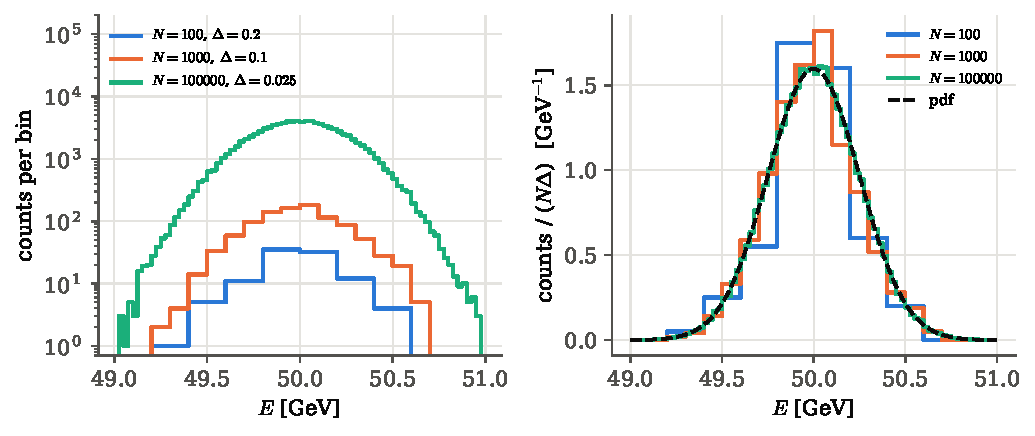
\includegraphics[width=0.95\linewidth]{figures/ch01/density_histogram.pdf}
\caption{Left: counts per bin for three data sets ($N=100$, $10^3$, $10^5$
with bins of 0.2, 0.1, 0.025 GeV). The heights are not comparable. Right: the
same histograms divided by $N\Delta$. They now fluctuate around one curve, the
Gaussian density, whose peak is above 1 per GeV.}
\label{1b:fig:density-histogram}
\end{figure}

With the finest bins the estimated peak density is $\OneBPeakEst\,\mathrm{GeV}^{-1}$
against the exact $\OneBPeakExact\,\mathrm{GeV}^{-1}$, and the fraction of
electrons within $\pm\sigma$ of 50 GeV is $\OneBFracOneSig$ (the Gaussian
value is 0.6827).

\pyfile[firstline=58,lastline=69,firstnumber=58]{code/ch01/11_density_histogram.py}{The empirical CDF is a sorted sample}

Lines 60--61 are the whole empirical CDF: sort the sample, and assign to the
$i$-th smallest value the height $i/N$. Lines 66--69 draw the quartiles as
the construction ``go across at height $q$, then down to the axis''. With
$N=1000$ the sample quartiles are $\OneBQoneSample$, $\OneBMedSample$,
$\OneBQthreeSample\,$GeV, against the exact $\OneBQoneExact$, $\OneBMedExact$,
$\OneBQthreeExact\,$GeV.

\begin{figure}[htbp]
\centering
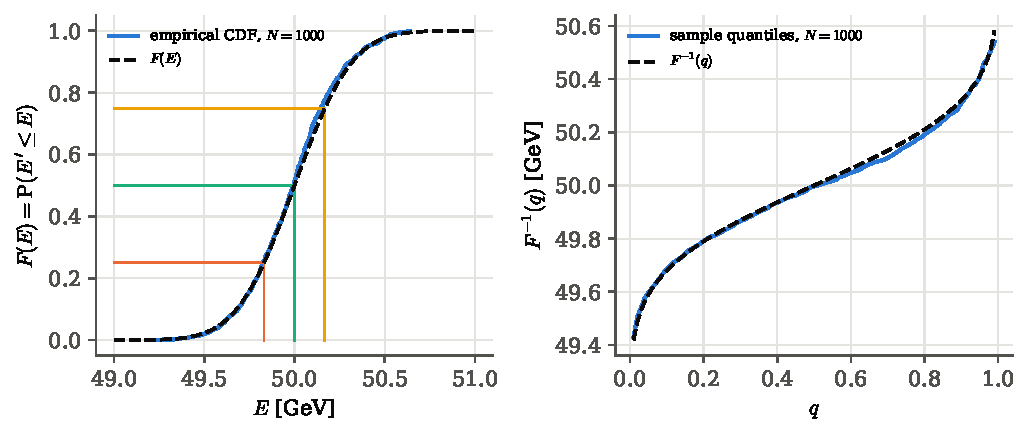
\includegraphics[width=0.95\linewidth]{figures/ch01/ecdf_quantiles.pdf}
\caption{Left: the empirical CDF of 1000 simulated energies (a staircase
with 1000 tiny steps) on top of the exact CDF. The coloured lines read off the
quartiles: across at $q=0.25,0.5,0.75$ and down to the energy axis. Right: the
same information turned sideways, sample quantiles against $q$, compared
with the exact quantile function.}
\label{1b:fig:ecdf}
\end{figure}

\paragraph{What this bought us.} Counts depend on how you bin. Densities do
not, but they carry units of $1/[x]$. The CDF needs no binning at all, which
is why tests that compare a sample to a model, such as Kolmogorov--Smirnov in
\cref{ch:04}, are built on the empirical CDF.

\paragraph{How research uses it.} Here the histogram \emph{verifies} a density
we already know. In research the direction is often reversed: nobody knows the
density of, say, the estimated tensor-to-scalar ratio after a realistic
foreground cleaning pipeline, so we simulate the whole pipeline many times and
the normalised histogram (or the empirical CDF) of the output \emph{is} our
best knowledge of its sampling distribution. Its quantiles become the error
bars. Chapters~\ref{ch:06} and~\ref{ch:08} do exactly this.
\section{Several variables at once: joint, marginal and conditional distributions}
\label{1b:sec:joint}

A calorimeter measures a photon. Two numbers describe the event: the true
energy $E$ that nature gave the photon, and the measured energy
$E_{\rm meas}=E+\text{noise}$ that the readout reports. The physics (a falling
spectrum from a decay or a background process) tells us how $E$ is
distributed. The detector response tells us how $E_{\rm meas}$ is spread for
a given $E$. But the histogram we actually fill contains only $E_{\rm meas}$.
The true energy is a \newterm{nuisance variable}: it is essential to the
physics of the measurement, and we never observe it.

The same situation appears in every cosmological analysis. A fit returns a
joint constraint on $(\Omega_m,\sigma_8)$, and a talk quotes
``$\Omega_m=0.31\pm0.01$'' with $\sigma_8$ ``marginalised over''. In both
cases we hold the joint distribution of several random variables and need
one of two operations. \emph{Marginalising} isolates one variable by
averaging out the others. \emph{Conditioning} fixes one variable and asks how
the rest are distributed. Neither is new. Both are rules from the first part
of \cref{ch:01} (the law of total probability and conditional probability),
applied to densities.

Two pictures make both operations concrete. Draw a scatter plot of many simulated pairs $(x,y)$. The density of points in
the plane is the joint density. Squash all the points onto the $x$ axis,
ignoring $y$, and histogram them: that is the marginal of $x$. Instead, keep
only the points in a thin vertical band at $x=x_0$, histogram their $y$
values and normalise: that is the conditional density of $y$ given $x_0$
\srcref{Cowan}{Figs.~1.4--1.6}. Projecting adds up all the ways a value of
$x$ could have arisen. Slicing throws away everything that disagrees with
what we know. This is the ``shrinking of the sample space'' of the first part
of this chapter.

So with two random variables there are four questions to ask.
\begin{enumerate}[leftmargin=1.5em,itemsep=1pt]
  \item How are the two variables distributed \emph{together}? (Joint.)
  \item How is one of them distributed if we do not care about, or cannot
        see, the other? (Marginal: average out the nuisance.)
  \item How is one distributed if we \emph{know} the value of the other?
        (Conditional: slice and renormalise.)
  \item Does knowing one change what we expect for the other? (If not, they
        are independent, and the joint is the product of the marginals.)
\end{enumerate}

\subsection{Joint distributions}

The other three questions are all answered from the distribution of the
pair taken together, so we define it first.

\begin{workdef}[joint mass function, joint density]
For discrete $X,Y$ the \newterm{joint mass function} is
$f(x,y)=\Prob(X=x,Y=y)$ \unpack{the probability that both statements hold at
once, $\Prob(X=x\text{ and }Y=y)$}. For continuous variables a
\newterm{joint density} is a function $f(x,y)\ge0$ with
$\iint f\,\dd x\,\dd y=1$ such that for every region $A$ of the plane
\[
  \Prob\bigl((X,Y)\in A\bigr)=\iint_A f(x,y)\,\dd x\,\dd y ,
\]
\unpack{probability per unit area, so $f(x,y)\,\dd x\,\dd y$ is the
probability of the small rectangle at $(x,y)$}. The joint CDF is
$F(x,y)=\Prob(X\le x,Y\le y)$.
\emph{Operational test:} a 2-D histogram of $N$ simulated pairs with cells
$\Delta x\times\Delta y$, divided by $N\Delta x\Delta y$, estimates $f(x,y)$.
Its units are $1/([x][y])$.
\end{workdef}

\oneBEx{A joint table and a uniform square}\label{1b:ex:joint-table}
Two binary variables with the joint table \mainref{Ex.~2.18, p.~31}
\begin{center}
\begin{tabular}{c|cc|c}
 & $Y=0$ & $Y=1$ & \\\hline
$X=0$ & 1/9 & 2/9 & 1/3\\
$X=1$ & 2/9 & 4/9 & 2/3\\\hline
 & 1/3 & 2/3 & 1
\end{tabular}
\end{center}
have $f(1,1)=\Prob(X=1,Y=1)=4/9$. The row and column sums written in the
margins of the table are the marginals of the next subsection. For a
continuous example, let
$(X,Y)$ be uniform on the unit square, $f=1$ there. Then
$\Prob(X<\tfrac12,Y<\tfrac12)$ is the integral of 1 over the lower-left
quarter, which is its area, $\tfrac14$.

\oneBEx{A density on a curved region}\label{1b:ex:parabola}
Let $f(x,y)=c\,x^2y$ on the region $x^2\le y\le1$ (and 0 elsewhere)
\mainref{Ex.~2.22, p.~32}. The region forces $-1\le x\le1$. Fix $c$ by
normalisation, integrating $y$ first at fixed $x$:
\begin{align*}
  1
  &\eqby{1} c\int_{-1}^{1}\!\!\int_{x^2}^{1}x^2y\,\dd y\,\dd x
   \eqby{2} c\int_{-1}^{1}x^2\,\frac{1-x^4}{2}\,\dd x
   \eqby{3} \frac c2\Bigl(\frac23-\frac27\Bigr)
   = \frac{4c}{21}
  \quad\Longrightarrow\quad c=\frac{21}{4}.
\end{align*}
\begin{explain}
  \item For each $x\in[-1,1]$, $y$ runs over $[x^2,1]$: this is the only
        delicate step, and \cref{1b:fig:parabola} is there to make it visible.
  \item $\int_{x^2}^1y\,\dd y=\tfrac12(1-x^4)$.
  \item $\int_{-1}^1x^2\dd x=\tfrac23$ and $\int_{-1}^1x^6\dd x=\tfrac27$.
\end{explain}
Now the probability that $X\ge Y$. Inside the support this needs $x\ge y\ge x^2$,
possible only for $0\le x\le1$ (the hatched sliver in the figure):
\begin{align*}
  \Prob(X\ge Y)
  &\eqby{1} \frac{21}{4}\int_0^1\!\!\int_{x^2}^{x}x^2y\,\dd y\,\dd x
   \eqby{2} \frac{21}{4}\int_0^1x^2\,\frac{x^2-x^4}{2}\,\dd x
   \eqby{3} \frac{21}{8}\Bigl(\frac15-\frac17\Bigr)
   = \frac{3}{20}.
\end{align*}
\begin{explain}
  \item The event $\{X\ge Y\}$ intersected with the support is
        $\{0\le x\le1,\ x^2\le y\le x\}$.
  \item $\int_{x^2}^{x}y\,\dd y=\tfrac12(x^2-x^4)$.
  \item $\int_0^1x^4=\tfrac15$, $\int_0^1x^6=\tfrac17$, and
        $\tfrac{21}{8}\cdot\tfrac{2}{35}=\tfrac{3}{20}$.
\end{explain}

\begin{figure}[htbp]
\centering
\begin{tikzpicture}[x=2.4cm,y=2.4cm]
  \fill[formblue!15] plot[domain=-1:1,samples=60] (\x,{\x*\x}) -- (1,1) -- (-1,1) -- cycle;
  \fill[pattern=crosshatch,pattern color=bdryred!70]
     plot[domain=0:1,samples=40] (\x,{\x*\x}) -- (0,0) -- cycle;
  \draw[->] (-1.35,0) -- (1.45,0) node[right,lbl] {$x$};
  \draw[->] (0,-0.1) -- (0,1.3) node[above,lbl] {$y$};
  \draw[thick,formblue] plot[domain=-1.1:1.1,samples=60] (\x,{\x*\x});
  \draw[thick,tangentgreen] (-0.05,-0.05) -- (1.2,1.2);
  \draw[faint] (-1,1) -- (1,1);
  \node[lbl,formblue,anchor=east] at (-1.12,1.12) {$y=x^2$};
  \node[lbl,tangentgreen,anchor=west] at (1.22,1.2) {$y=x$};
  \node[lbl,anchor=east] at (-0.02,1.06) {$1$};
  \node[lbl,anchor=north] at (1,-0.02) {$1$};
  \node[lbl,anchor=north] at (-1,-0.02) {$-1$};
  \node[lbl,align=center] at (-0.58,0.62) {support\\$x^2\le y\le1$};
  \draw[bdryred,->] (1.05,0.35) -- (0.62,0.5);
  \node[lbl,bdryred,anchor=west] at (1.05,0.35) {$\{X\ge Y\}$};
\end{tikzpicture}
\caption{The density $\tfrac{21}{4}x^2y$ lives on the shaded region between
the parabola $y=x^2$ and the line $y=1$. The event $X\ge Y$ is the hatched
sliver between the parabola and the diagonal $y=x$. To integrate, fix $x$
and let $y$ run up the vertical segment inside the region.}
\label{1b:fig:parabola}
\end{figure}

\subsection{Marginal distributions: averaging out the nuisance}\label{1b:sec:marginal}

If we only care about $X$, the event ``$X=x$'' is the disjoint union of the
events ``$X=x$ and $Y=y$'' over all values $y$. The law of total probability
(first part of \cref{ch:01}) adds them up.

\begin{workdef}[marginal distribution]
The \newterm{marginal} mass function or density of $X$ is
\[
  f_X(x)=\sum_yf(x,y)\quad\text{(discrete)},\qquad
  f_X(x)=\int_{-\infty}^{\infty}f(x,y)\,\dd y\quad\text{(continuous)},
\]
and similarly $f_Y(y)=\sum_xf(x,y)$ or $\int f(x,y)\,\dd x$
\unpack{sum or integrate the joint over every value of the variable we want
to get rid of}. The variable summed over is \emph{marginalised} or
\emph{integrated out}.
\emph{Operational test:} simulate pairs $(x,y)$, throw away the $y$'s, and
histogram the $x$'s.
\end{workdef}

We need a marginal distribution to isolate and understand the probability of
a single variable by averaging out or removing ``nuisance'' variables from a
complex joint distribution. The word ``averaging'' is meant literally.
Write the joint as $f(x,y)=f(x\given y)f_Y(y)$ (the product rule, derived
below). Then the marginal $f_X(x)=\int f(x\given y)f_Y(y)\dd y$ is the
average of the conditional densities $f(x\given y)$, each weighted by how
probable its nuisance value $y$ is.

Why is the continuous marginal an integral over $y$
\srcref{Cowan}{(1.20)--(1.21)}? Cut the vertical strip $[x,x+\dd x]$ into
small cells of height $\Delta y$ at heights $y_i$:
\begin{align*}
  \Prob\bigl(x\le X\le x+\dd x\bigr)
  &\eqby{1} \sum_i\Prob\bigl(x\le X\le x+\dd x,\ y_i\le Y\le y_i+\Delta y\bigr)
  \\
  &\eqby{2} \sum_i f(x,y_i)\,\Delta y\,\dd x
   \;\xrightarrow{\ \Delta y\to0\ }\;\Bigl[\int f(x,y)\,\dd y\Bigr]\dd x .
\end{align*}
\begin{explain}
  \item The cells are disjoint and together make up the strip (the law of
        total probability).
  \item The probability of a small cell is the joint density times its area.
\end{explain}
The bracket is probability per unit $x$: the marginal density.

\oneBEx{Margins of a table, and what they cannot tell you}\label{1b:ex:margins}
For the table \mainref{Ex.~2.24, p.~33}
\begin{center}
\begin{tabular}{c|cc|c}
 & $Y=0$ & $Y=1$ & \\\hline
$X=0$ & 1/10 & 2/10 & 3/10\\
$X=1$ & 3/10 & 4/10 & 7/10\\\hline
 & 4/10 & 6/10 & 1
\end{tabular}
\end{center}
the marginal of $X$ is the column of row sums, $f_X(0)=3/10$, $f_X(1)=7/10$,
and the marginal of $Y$ is the row of column sums. The name ``marginal''
literally means ``written in the margin of the table''.

Marginals lose information. The joint table
$f(0,0)=\tfrac1{12}$, $f(1,0)=\tfrac5{12}$, $f(0,1)=f(1,1)=\tfrac3{12}$ has
marginals $f_X=(\tfrac13,\tfrac23)$ and $f_Y=(\tfrac12,\tfrac12)$. So does the
different table $f(0,0)=\tfrac16$, $f(1,0)=\tfrac13$, $f(0,1)=\tfrac16$,
$f(1,1)=\tfrac13$ \srcref{CasellaBerger}{Ex.~4.1.9}. Knowing both marginals
does not determine the joint. This is a small instance of a big theme:
summarising discards information. A CMB power spectrum $\Cell$ is a
``marginal'' summary that keeps the variance at each scale and throws away
the phases, and \cref{ch:12} is about recovering some of what was thrown
away.

\oneBEx{Marginal densities by integration}\label{1b:ex:marginal-integrals}
\begin{itemize}[leftmargin=1.2em,itemsep=1pt]
  \item $f(x,y)=e^{-(x+y)}$ for $x,y\ge0$:
        $f_X(x)=e^{-x}\int_0^\infty e^{-y}\dd y=e^{-x}$ \mainref{Ex.~2.26}.
  \item $f(x,y)=x+y$ on the unit square:
        $f_Y(y)=\int_0^1(x+y)\dd x=\tfrac12+y$ \mainref{Ex.~2.27}.
  \item $f(x,y)=\tfrac{21}{4}x^2y$ on $x^2\le y\le1$ (\cref{1b:ex:parabola}):
        \begin{align*}
          f_X(x)
          \eqby{1} \frac{21}{4}x^2\int_{x^2}^{1}y\,\dd y
          = \frac{21}{8}x^2(1-x^4),\qquad -1\le x\le1 .
        \end{align*}
        \begin{explain}
          \item At fixed $x$ the density is nonzero only for $x^2\le y\le1$,
                so those are the limits of the $y$ integral
                \mainref{Ex.~2.28, p.~34}.
        \end{explain}
\end{itemize}
In the last case the limits of integration depend on $x$. Forgetting that is
the commonest error in marginalisation.

\subsection{The Gaussian case: marginalising by completing the square}

The single most important joint density is the bivariate Gaussian. With zero
means, standard deviations $\sigma_x,\sigma_y$ and a correlation parameter
$\rho\in(-1,1)$ (\cref{1b:sec:covariance} shows that $\rho$ is the
correlation coefficient),
\begin{equation}
  f(x,y)=\frac{1}{2\pi\sigma_x\sigma_y\sqrt{1-\rho^2}}
  \exp\Bigl\{-\frac{1}{2(1-\rho^2)}
  \Bigl[\frac{x^2}{\sigma_x^2}-\frac{2\rho xy}{\sigma_x\sigma_y}
  +\frac{y^2}{\sigma_y^2}\Bigr]\Bigr\}.
  \label{1b:eq:bvn}
\end{equation}
The contours of $f$ are ellipses, tilted when $\rho\ne0$. We need one integral,
the Gaussian integral
$\int_{-\infty}^{\infty}e^{-(y-m)^2/(2s^2)}\dd y=\sqrt{2\pi}\,s$
(for any shift $m$ and width $s>0$).

\oneBEx{The marginal and the conditional of a bivariate Gaussian}\label{1b:ex:bvn-marginal}
The question: how is $X$ distributed on its own, and how is $Y$ distributed
once $X=x$ is known? The plan is to rewrite the exponent so that $y$ appears
in a single square. Then the $y$ integral becomes the Gaussian integral just
recalled. First rearrange the bracket in \eqref{1b:eq:bvn}:
\begin{align*}
  \frac{x^2}{\sigma_x^2}-\frac{2\rho xy}{\sigma_x\sigma_y}+\frac{y^2}{\sigma_y^2}
  &\eqby{1} \Bigl(\frac{y}{\sigma_y}-\frac{\rho x}{\sigma_x}\Bigr)^2
            +\frac{x^2}{\sigma_x^2}-\frac{\rho^2x^2}{\sigma_x^2}
   = \frac{\bigl(y-\rho\sigma_yx/\sigma_x\bigr)^2}{\sigma_y^2}
            +(1-\rho^2)\frac{x^2}{\sigma_x^2}.
\end{align*}
\begin{explain}
  \item Expanding $(y/\sigma_y-\rho x/\sigma_x)^2$ gives
        $y^2/\sigma_y^2-2\rho xy/(\sigma_x\sigma_y)+\rho^2x^2/\sigma_x^2$,
        so we must add back $(1-\rho^2)x^2/\sigma_x^2$ to restore the
        original expression.
\end{explain}
Dividing by $2(1-\rho^2)$ and writing $m(x)=\rho\sigma_yx/\sigma_x$ and
$s=\sigma_y\sqrt{1-\rho^2}$, the joint density factorises as
\[
  f(x,y)=\frac{1}{2\pi\sigma_x s}
  \exp\Bigl[-\frac{(y-m(x))^2}{2s^2}\Bigr]\exp\Bigl[-\frac{x^2}{2\sigma_x^2}\Bigr].
\]
The marginal of $X$ follows:
\begin{align*}
  f_X(x)
  &\eqby{1} \frac{e^{-x^2/2\sigma_x^2}}{2\pi\sigma_xs}
     \int_{-\infty}^{\infty}e^{-(y-m(x))^2/2s^2}\,\dd y
   \eqby{2} \frac{e^{-x^2/2\sigma_x^2}}{2\pi\sigma_xs}\,\sqrt{2\pi}\,s
   = \frac{1}{\sqrt{2\pi}\,\sigma_x}e^{-x^2/2\sigma_x^2}.
\end{align*}
\begin{explain}
  \item Definition of the marginal. The factor depending only on $x$ comes
        out of the $y$ integral.
  \item Gaussian integral with shift $m(x)$ and width $s$. The shift does not
        change the area, which is why the answer is so simple.
\end{explain}
So $X\sim\Normal(0,\sigma_x^2)$ whatever $\rho$ is, and by the symmetry of
\eqref{1b:eq:bvn}, $Y\sim\Normal(0,\sigma_y^2)$. The conditional density of
$Y$ at fixed $X=x$ is the joint divided by the marginal (defined in the next
subsection):
\[
  f(y\given x)=\frac{f(x,y)}{f_X(x)}
  =\frac{1}{\sqrt{2\pi}\,s}\exp\Bigl[-\frac{(y-\rho\sigma_yx/\sigma_x)^2}{2s^2}\Bigr],
  \qquad
  Y\given X=x\ \sim\ \Normal\Bigl(\rho\frac{\sigma_y}{\sigma_x}x,\
  \sigma_y^2(1-\rho^2)\Bigr).
\]
Knowing $X$ does two things to $Y$: it shifts the centre along the line
$y=\rho\sigma_yx/\sigma_x$ (the ``regression line''), and it shrinks the
width by the factor $\sqrt{1-\rho^2}$. For $\rho=0.7$ that factor is $0.71$.

\begin{pitfall}[Marginal width is not conditional width]
In a two-parameter fit, the error bar on one parameter with the other held
fixed at its best value is the \emph{conditional} width
$\sigma_y\sqrt{1-\rho^2}$. The error bar with the other parameter
marginalised is $\sigma_y$. For strongly correlated parameters these differ a
lot: $\rho=0.95$ gives a factor $3.2$. Quoting the conditional error as if it
were the marginal one is a classic way to overstate a result. \Cref{ch:10}
meets the same distinction as $1/\sqrt{\Fish_{ii}}$ versus
$\sqrt{(\Fish^{-1})_{ii}}$.
\end{pitfall}

\subsection{Conditional distributions: slicing and renormalising}

Slicing the scatter plot at $Y=y$ and renormalising the slice gives the
definition.

\begin{workdef}[conditional mass function and density]
For discrete variables, the \newterm{conditional mass function} of $X$ given
$Y=y$ is
\[
  f_{X|Y}(x\given y)=\Prob(X=x\given Y=y)=\frac{f(x,y)}{f_Y(y)},
  \qquad f_Y(y)>0 ,
\]
the ordinary conditional probability of the first part of \cref{ch:01}. For
continuous variables the \newterm{conditional density} is defined by the same
formula \unpack{the joint along the line $Y=y$, divided by its total, so
that it integrates to 1 over $x$}, and
$\Prob(X\in A\given Y=y)=\int_Af_{X|Y}(x\given y)\,\dd x$.
\emph{Operational test:} keep only simulated pairs with $y$ in a thin band
around $y_0$, histogram their $x$ values and normalise.
\end{workdef}

In the continuous case the event $\{Y=y\}$ has probability zero. So
conditioning on it cannot literally mean $\Prob(A\cap B)/\Prob(B)$, which
would be $0/0$. Why is the definition still right? Think of a thin band of
width $\dd y$ around $y$. Both numerator and denominator carry the same
factor $\dd y$, which cancels and leaves the ratio of densities
\srcref{Cowan}{(1.23)}. (Wasserman \mainref{p.~36, footnote 6} calls
conditioning on a probability-zero event ``treading in deep water'' and
simply adopts the formula as the definition.) Rearranging the definition
gives the product rule
\begin{equation}
  f(x,y)=f_{X|Y}(x\given y)\,f_Y(y)=f_{Y|X}(y\given x)\,f_X(x),
  \label{1b:eq:product-rule}
\end{equation}
and from it the continuous law of total probability and Bayes' theorem
\srcref{Cowan}{(1.26)--(1.28)}:
\begin{equation}
  f_X(x)=\int f_{X|Y}(x\given y)f_Y(y)\,\dd y,
  \qquad
  f_{Y|X}(y\given x)=\frac{f_{X|Y}(x\given y)\,f_Y(y)}{\int f_{X|Y}(x\given y')f_Y(y')\,\dd y'} .
  \label{1b:eq:cont-bayes}
\end{equation}
The first is ``sum over the branches of a tree'', with a continuum of
branches. The second reads the tree backwards. With $y$ a parameter and $x$
the data, $f_{X|Y}$ is the prediction and $f_{Y|X}$ the inference: this is
the equation \cref{ch:05} is built on.

\oneBEx{Conditional probabilities from a density}\label{1b:ex:conditional}
\begin{enumerate}[label=(\alph*),leftmargin=1.6em,itemsep=2pt]
  \item $f(x,y)=x+y$ on the unit square, with $f_Y(y)=y+\tfrac12$
        (\cref{1b:ex:marginal-integrals}). Then $f(x\given y)=(x+y)/(y+\tfrac12)$
        and \mainref{Ex.~2.38, p.~37}
        \begin{align*}
          \Prob\bigl(X<\tfrac14\given Y=\tfrac13\bigr)
          &\eqby{1} \int_0^{1/4}\frac{x+\frac13}{\frac13+\frac12}\,\dd x
           \eqby{2} \frac65\Bigl[\frac{x^2}{2}+\frac{x}{3}\Bigr]_0^{1/4}
           = \frac65\Bigl(\frac1{32}+\frac1{12}\Bigr)
           = \frac{11}{80}.
        \end{align*}
        \begin{explain}
          \item Integrate the conditional density over the event, at $y=\tfrac13$.
          \item $1/(\tfrac13+\tfrac12)=\tfrac65$, and the antiderivative is
                elementary. Then $\tfrac1{32}+\tfrac1{12}=\tfrac{11}{96}$.
        \end{explain}
  \item Build a joint from a marginal and a conditional: $X\sim$ Uniform$(0,1)$
        and then $Y\given X=x\sim$ Uniform$(x,1)$ \mainref{Ex.~2.39}. Then
        $f(y\given x)=1/(1-x)$ for $x<y<1$, and by \eqref{1b:eq:product-rule}
        $f(x,y)=1/(1-x)$ on $0<x<y<1$. The marginal of $Y$ is
        \begin{align*}
          f_Y(y)
          &\eqby{1} \int_0^y\frac{\dd x}{1-x}
           \eqby{2} -\int_1^{1-y}\frac{\dd u}{u}
           = -\ln(1-y),\qquad 0<y<1 .
        \end{align*}
        \begin{explain}
          \item At fixed $y$, the joint is nonzero for $0<x<y$.
          \item Substitute $u=1-x$, $\dd u=-\dd x$; the limits $x=0,y$ become
                $u=1,1-y$.
        \end{explain}
        The density of $Y$ rises towards $y=1$: each stage pushes $Y$ upward.
  \item For $f=\tfrac{21}{4}x^2y$ on $x^2\le y\le1$, dividing by the
        marginal of \cref{1b:ex:marginal-integrals} gives
        $f(y\given x)=2y/(1-x^4)$ on $x^2\le y\le1$. At $x=\tfrac12$ this is
        $32y/15$, and \mainref{Ex.~2.40, p.~38}
        \begin{align*}
          \Prob\bigl(Y\ge\tfrac34\given X=\tfrac12\bigr)
          \eqby{1} \int_{3/4}^{1}\frac{32y}{15}\,\dd y
          = \frac{16}{15}\Bigl(1-\frac{9}{16}\Bigr)=\frac{7}{15}.
        \end{align*}
        \begin{explain}
          \item The conditional density at $x=\tfrac12$ lives on
                $\tfrac14\le y\le1$, and the event asks for the top part.
        \end{explain}
\end{enumerate}

\subsection{Independence}

The last question is whether slicing changes anything at all. If every slice
looks the same, learning one variable teaches us nothing about the other.

\begin{workdef}[independent random variables]
$X$ and $Y$ are \newterm{independent}, written $X\perp Y$, if for every pair
of sets $A,B$
\[
  \Prob(X\in A,\ Y\in B)=\Prob(X\in A)\,\Prob(Y\in B)
\]
\unpack{every event about $X$ is independent of every event about $Y$}.
Equivalently the joint factorises into the marginals,
$f(x,y)=f_X(x)f_Y(y)$ for all $x,y$ \mainref{Thm~2.30, p.~35}, and then
$f(y\given x)=f_Y(y)$: learning $x$ does not change the distribution of $Y$.
\emph{Operational test:} slice the scatter plot at several $x$ values. If
the normalised $y$-histograms in the slices all look the same, and the same
as the marginal, the variables are independent.
\end{workdef}

\oneBEx{Checking independence}\label{1b:ex:independence}
\begin{enumerate}[label=(\alph*),leftmargin=1.6em,itemsep=2pt]
  \item The table with all four entries $\tfrac14$ is independent:
        $f_X=f_Y=(\tfrac12,\tfrac12)$ and every cell equals
        $\tfrac12\cdot\tfrac12$. The table $f(0,0)=f(1,1)=\tfrac12$,
        $f(0,1)=f(1,0)=0$ has the \emph{same} marginals but is not independent:
        $f_X(0)f_Y(1)=\tfrac14\ne0=f(0,1)$ \mainref{Ex.~2.31}.
  \item $X,Y$ independent with the same density $f(x)=2x$ on $[0,1]$. The
        joint is $4xy$ on the unit square, and \mainref{Ex.~2.32}
        \begin{align*}
          \Prob(X+Y\le1)
          &\eqby{1} 4\int_0^1x\Bigl[\int_0^{1-x}y\,\dd y\Bigr]\dd x
           \eqby{2} 2\int_0^1x(1-x)^2\,\dd x
           \eqby{3} 2\Bigl(\frac12-\frac23+\frac14\Bigr)=\frac16 .
        \end{align*}
        \begin{explain}
          \item The event is the triangle below the line $y=1-x$; for each $x$,
                $y$ runs from 0 to $1-x$.
          \item $\int_0^{1-x}y\,\dd y=\tfrac12(1-x)^2$.
          \item Expand $x(1-x)^2=x-2x^2+x^3$ and integrate term by term.
        \end{explain}
  \item Shortcut \mainref{Thm~2.33, p.~36}: if the joint is nonzero on a
        rectangle (possibly infinite) and has the form $g(x)h(y)$, the
        variables are independent. $f=2e^{-(x+2y)}$ on $x,y>0$ is
        $g(x)h(y)$ with $g=2e^{-x}$, $h=e^{-2y}$, so $X\perp Y$.
  \item The rectangle condition matters. $\tfrac{21}{4}x^2y$ on $x^2\le y\le1$
        looks like $g(x)h(y)$, but the region is not a rectangle, and
        $f(y\given x)=2y/(1-x^4)$ depends on $x$: learning $x$ tells us $y\ge
        x^2$. $X$ and $Y$ are dependent.
\end{enumerate}

For more than two variables the definitions carry over. A
\newterm{random vector} $\bm X=(X_1,\dots,X_n)$ has a joint density
$f(x_1,\dots,x_n)$; marginals integrate out any subset of components;
$X_1,\dots,X_n$ are independent if $f=\prod_if_{X_i}(x_i)$. If they are
independent \emph{and} all have the same marginal $F$ they are
\newterm{iid} (independent and identically distributed), written
$X_1,\dots,X_n\iid F$, and form a \newterm{random sample} of size $n$ from
$F$ \mainref{Def.~2.41, p.~39}. Repeated measurements, Monte Carlo draws and
the pixels of a white-noise map are the standard iid examples.

Two multivariate models recur throughout the book \mainref{\S2.10}. The
\newterm{multinomial} counts how $n$ independent draws fall into $k$
categories (histogram bins) with probabilities $p_1,\dots,p_k$. The marginal
of one count $X_j$ is Binomial$(n,p_j)$: lump all the other categories into
``not $j$'' and each draw becomes a Bernoulli$(p_j)$ trial. The
\newterm{multivariate normal} $\Normal(\bm\mu,\Sigma)$ has density
\begin{equation}
  f(\bm x)=\frac{1}{(2\pi)^{k/2}\abs{\Sigma}^{1/2}}
  \exp\Bigl\{-\tfrac12(\bm x-\bm\mu)\T\Sigma^{-1}(\bm x-\bm\mu)\Bigr\},
  \label{1b:eq:mvn}
\end{equation}
with $\Sigma$ a symmetric positive-definite $k\times k$ matrix. For $k=2$ and
$\Sigma=\bigl(\begin{smallmatrix}\sigma_x^2&\rho\sigma_x\sigma_y\\
\rho\sigma_x\sigma_y&\sigma_y^2\end{smallmatrix}\bigr)$ it reduces to
\eqref{1b:eq:bvn}:
\begin{align*}
  \abs{\Sigma}
  &\eqby{1} \sigma_x^2\sigma_y^2(1-\rho^2),\qquad
  \Sigma^{-1}\eqby{2}\frac{1}{\sigma_x^2\sigma_y^2(1-\rho^2)}
   \begin{pmatrix}\sigma_y^2&-\rho\sigma_x\sigma_y\\-\rho\sigma_x\sigma_y&\sigma_x^2\end{pmatrix},\\
  \bm x\T\Sigma^{-1}\bm x
  &\eqby{3} \frac{\sigma_y^2x^2-2\rho\sigma_x\sigma_yxy+\sigma_x^2y^2}{\sigma_x^2\sigma_y^2(1-\rho^2)}
   = \frac{1}{1-\rho^2}\Bigl[\frac{x^2}{\sigma_x^2}-\frac{2\rho xy}{\sigma_x\sigma_y}+\frac{y^2}{\sigma_y^2}\Bigr].
\end{align*}
\begin{explain}
  \item Determinant of a $2\times2$ matrix, $ad-bc$.
  \item Inverse of a $2\times2$ matrix: swap the diagonal, negate the
        off-diagonal, divide by the determinant.
  \item Multiply out $(x,y)\,\Sigma^{-1}(x,y)\T$, then divide numerator and
        denominator by $\sigma_x^2\sigma_y^2$.
\end{explain}
The general marginal and conditional rules \mainref{Thm~2.44, p.~40},
$X_b\given X_a=x_a\sim\Normal\bigl(\mu_b+\Sigma_{ba}\Sigma_{aa}^{-1}(x_a-\mu_a),\,
\Sigma_{bb}-\Sigma_{ba}\Sigma_{aa}^{-1}\Sigma_{ab}\bigr)$, reduce for $k=2$ to
exactly what we derived in \cref{1b:ex:bvn-marginal}:
$\Sigma_{ba}\Sigma_{aa}^{-1}=\rho\sigma_x\sigma_y/\sigma_x^2=\rho\sigma_y/\sigma_x$
and $\Sigma_{bb}-\Sigma_{ba}^2/\Sigma_{aa}=\sigma_y^2(1-\rho^2)$. The general
proofs are in \cref{ch:02}.

\subsection{Seeing it: projections, slices, and the smeared spectrum}

The first script samples the bivariate Gaussian with $\sigma_x=1$,
$\sigma_y=2$, $\rho=0.7$, projects, and slices at $x_0=1$.

\pyfile[firstline=23,lastline=34,firstnumber=23]{code/ch01/12_marginal_gaussian.py}{Marginal by projection, conditional by slicing}

Line 26 draws $\OneBMargN$ pairs from $\Normal(\bm0,\Cmat)$. The marginal needs
no code at all: \texttt{Y} on its own \emph{is} a sample from $f_Y$ (line 27
just splits the columns). The conditional is a boolean mask, the band
$\abs{x-1}<0.05$ (line 31), exactly the ``conditioning is selecting a
subset'' of the first part of \cref{ch:01}.

\begin{figure}[htbp]
\centering
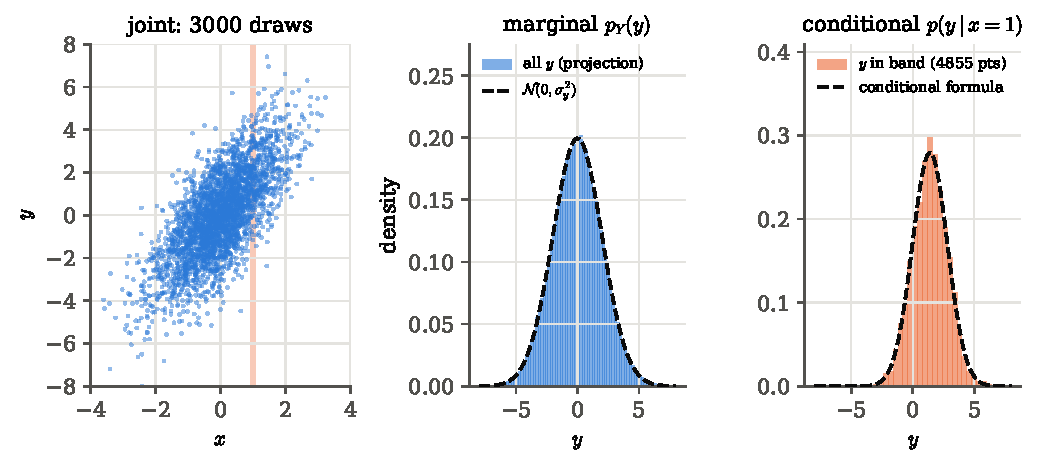
\includegraphics[width=\linewidth]{figures/ch01/marginal_gaussian.pdf}
\caption{Left: 3000 draws from the correlated Gaussian, with the thin band at
$x=1$ shaded. Middle: all $y$ values, projected onto the $y$ axis, follow the
marginal $\Normal(0,4)$. Right: only the $y$ values from inside the band,
renormalised, follow the narrower and shifted conditional density.}
\label{1b:fig:marginal-gaussian}
\end{figure}

The simulated marginal widths are $\OneBMargSdX$ and $\OneBMargSdY$ (exact 1
and 2). The band holds $\OneBBandN$ points, whose $y$ values have mean
$\OneBCondMeanSim$ and standard deviation $\OneBCondSdSim$, against the exact
conditional $\rho\sigma_yx_0/\sigma_x=\OneBCondMeanExact$ and
$\sigma_y\sqrt{1-\rho^2}=\OneBCondSdExact$ (the band has finite width, which
adds a tiny extra spread).

\oneBEx{The measured spectrum: marginalising the true energy}\label{1b:ex:smearing}
Return to the photon in the calorimeter from the start of this section. Its
true energy $E$ is never observed. Only the measured energy
$E_{\rm meas}=E+\text{noise}$ is recorded, and we want the spectrum of
$E_{\rm meas}$. Let the true energy be exponential,
$f(E)=e^{-E/\beta}/\beta$ for $E>0$ with $\beta=20\,$GeV (a falling
spectrum), and the detector Gaussian,
$f(x\given E)=\exp[-(x-E)^2/2\sigma^2]/(\sqrt{2\pi}\sigma)$ with
$\sigma=5\,$GeV, where $x=E_{\rm meas}$. The joint is the product
\eqref{1b:eq:product-rule}, and the spectrum we histogram is the marginal
\begin{equation}
  f(x)=\int_0^\infty\frac{e^{-E/\beta}}{\beta}\,
  \frac{e^{-(x-E)^2/2\sigma^2}}{\sqrt{2\pi}\,\sigma}\,\dd E .
  \label{1b:eq:smear-integral}
\end{equation}
To do the integral, collect the $E$-dependence of the exponent into one
square, so that what is left is a Gaussian integral:
\begin{align*}
  -\frac{E}{\beta}-\frac{(x-E)^2}{2\sigma^2}
  &\eqby{1} -\frac{E^2-2E\bigl(x-\sigma^2/\beta\bigr)+x^2}{2\sigma^2}
   \eqby{2} -\frac{\bigl(E-m\bigr)^2}{2\sigma^2}+\frac{m^2-x^2}{2\sigma^2}\\
  &\eqby{3} -\frac{\bigl(E-m\bigr)^2}{2\sigma^2}-\frac{x}{\beta}+\frac{\sigma^2}{2\beta^2},
\end{align*}
with $m=x-\sigma^2/\beta$.
\begin{explain}
  \item Put both terms over $2\sigma^2$: $E/\beta=2\sigma^2E/(2\sigma^2\beta)$,
        and expand $(x-E)^2$.
  \item Complete the square, $E^2-2Em=(E-m)^2-m^2$.
  \item $m^2-x^2=-2x\sigma^2/\beta+\sigma^4/\beta^2$; divide by $2\sigma^2$.
\end{explain}
The last two terms do not involve $E$ and leave the integral. What remains is
a Gaussian in $E$ centred at $m$, integrated over $E>0$ only:
\begin{align*}
  f(x)
  &\eqby{1} \frac1\beta\,e^{\sigma^2/2\beta^2-x/\beta}
     \int_0^\infty\frac{e^{-(E-m)^2/2\sigma^2}}{\sqrt{2\pi}\,\sigma}\dd E
   \eqby{2} \frac1\beta\,e^{\sigma^2/2\beta^2-x/\beta}\,
     \Phi\Bigl(\frac{x-\sigma^2/\beta}{\sigma}\Bigr).
\end{align*}
\begin{explain}
  \item Insert the rearranged exponent into \eqref{1b:eq:smear-integral}.
  \item The remaining integral is $\Prob(W>0)$ for $W\sim\Normal(m,\sigma^2)$,
        which is $\Prob\bigl((W-m)/\sigma>-m/\sigma\bigr)=1-\Phi(-m/\sigma)=\Phi(m/\sigma)$
        by the symmetry of the standard Gaussian.
\end{explain}
The formula shows two things. First, far above the resolution scale,
$x\gg\sigma^2/\beta+\sigma$, we have $\Phi\to1$. There the measured spectrum
is the true exponential with the same slope, multiplied by the constant
$e^{\sigma^2/2\beta^2}>1$. Smearing ``feeds'' events from low to high energy,
and so raises the tail. Second, near and below zero the $\Phi$ factor cuts
in. There is a finite probability of measuring a \emph{negative} energy,
which no true photon has.

\pyfile[firstline=24,lastline=34,firstnumber=24]{code/ch01/13_detector_smearing.py}{Simulating the nuisance, then forgetting it}

Lines 26--27 are the whole physics: draw the true energy, add the noise.
Marginalising over the nuisance then costs nothing: we simply never look at
\texttt{E\_true} again. The function \texttt{p\_meas} (lines 30--33) is the
closed form just derived.

\begin{figure}[htbp]
\centering
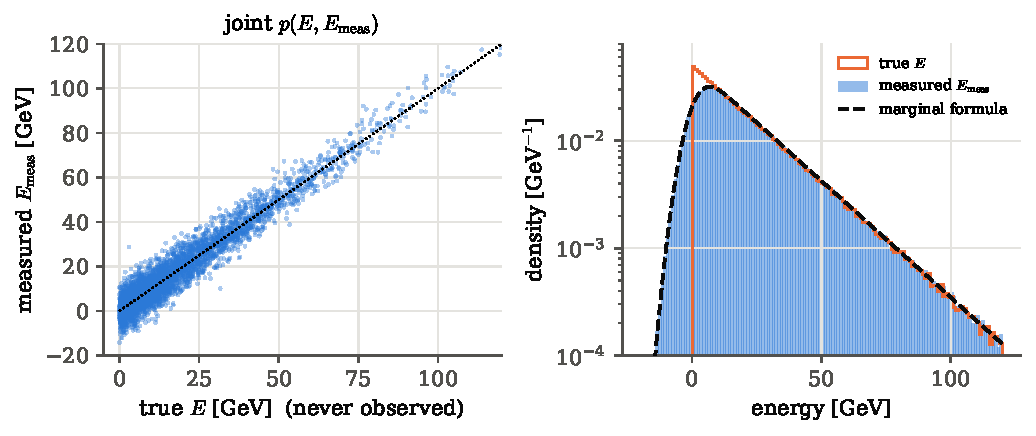
\includegraphics[width=0.95\linewidth]{figures/ch01/detector_smearing.pdf}
\caption{Left: the joint distribution of (true, measured) energy, scattered
around the diagonal. Only the vertical coordinate is ever recorded. Right, on a
log scale: the true spectrum (orange outline) is a straight line starting at
zero. The measured spectrum (blue) is its marginal with the true energy
integrated out. It leaks below zero and runs parallel to, and slightly above,
the true line in the tail. The dashed curve is the closed form.}
\label{1b:fig:smearing}
\end{figure}

With $\OneBSmearN$ photons the simulation gives a mean measured energy of
$\OneBSmearMeanSim\,$GeV (exact $\beta=20$), a variance of
$\OneBSmearVarSim\,\mathrm{GeV}^2$ (exact $\beta^2+\sigma^2=\OneBSmearVarExact$,
derived in \cref{1b:sec:expectation}), and a fraction
$\OneBSmearNegSim$ of negative measured energies (exact
$\int_{-\infty}^0f=\OneBSmearNegExact$). A $\chi^2$ comparison of the
histogram with the bin-integrated formula gives $\OneBSmearChi$ for
$\OneBSmearNdf$ bins, which is what agreement looks like (\cref{ch:04} makes
this precise).

\paragraph{What this bought us.} Marginalising a nuisance variable is, in simulation, the act of not looking
at it. Analytically it is an integral over the joint, $f(x)=\int f(x\given
E)f(E)\,\dd E$. The same integral with $E$ a parameter is the Bayesian
evidence of \cref{ch:05}, and with $E$ the true sky it is the forward model
of \cref{ch:08}.

\begin{inpractice}[Verification here, forward modelling in research]
The closed form above \emph{verifies} the simulation. In a real calorimeter
the response $f(x\given E)$ has non-Gaussian tails, depends on position and
is known only through test-beam data and detector simulation. Then the
marginal $\int f(x\given E)f(E\given\theta)\,\dd E$ has no closed form and
is computed by exactly the two lines of code above, repeated for each
theory parameter $\theta$. That forward-folded spectrum is what a fit
compares with data. Going the other way, from $x$ back to $E$, is
\emph{unfolding}, a conditional distribution $f(E\given x)$ computed with
\eqref{1b:eq:cont-bayes}.
\end{inpractice}
\section{Functions of random variables: change of variables and Jacobians}
\label{1b:sec:transform}

A classical harmonic oscillator swings as $x(t)=A\cos\omega t$. We take a
photograph at a random moment, with no idea of the phase. Where is the bob
most likely to be caught? The motion is completely deterministic; the only
randomness is \emph{when} we look, and the time $t$ is uniform over a period.
The position is a function of that uniform time, $X=A\cos\omega T$, so its
distribution is fixed by the distribution of $T$ and the function. We will
find that the bob is most likely near the turning points, where it moves
slowly, and least likely at the centre, where it is fastest.

The same question appears whenever an observable is a function of something
whose distribution we know: the angle of a decay product, the transverse
momentum computed from that angle, a flux from a magnitude, the logarithm of
a likelihood. In each case we know the density of $X$ and want the density of
$Y=r(X)$. The tool is the Jacobian, and it works for several variables at
once. The oscillator has a second use: histogramming $x(t)$ at random times is
the same act as histogramming samples from a posterior (\cref{ch:05}).

The key idea is that probability is conserved when we relabel. Think of probability as a fluid of total mass 1 spread along the $x$ axis.
The map $y=r(x)$ moves each drop of fluid to a new place but creates and
destroys nothing. Whatever mass sat in $[x,x+\dd x]$ now sits in the image
interval $[y,y+\dd y]$. If the map stretches that interval
($\abs{\dd y}>\abs{\dd x}$), the same mass is spread thinner and the density
drops. If it compresses it, the density rises. For the oscillator the
``map'' is from time to position: near the turning points a long stretch of
time maps onto a short stretch of position, so the density of position is
high there. This is the same bookkeeping as a number density $n(\bm x)$
under a change of coordinates, or a phase-space density under a canonical
transformation.

In practice we find the distribution of $Y=r(X)$ in three steps.
\begin{enumerate}[leftmargin=1.5em,itemsep=1pt]
  \item For a value $y$, which values of $x$ produce $Y\le y$? Draw it.
  \item The probability of $Y\le y$ is the probability of that set of $x$'s.
        That is the CDF of $Y$.
  \item Differentiate to get the density. If $r$ is one-to-one, this collapses
        to ``old density times $\abs{\dd x/\dd y}$''. If several $x$'s give the
        same $y$, add their contributions.
\end{enumerate}

\subsection{Discrete variables: collect the preimages}

For a discrete $X$, $Y=r(X)$ is discrete and
$\Prob(Y=y)=\Prob\bigl(X\in r^{-1}(y)\bigr)$, where $r^{-1}(y)$ is the set of
all $x$ with $r(x)=y$. If $\Prob(X=-1)=\Prob(X=1)=\tfrac14$,
$\Prob(X=0)=\tfrac12$ and $Y=X^2$, then $\Prob(Y=0)=\Prob(X=0)=\tfrac12$ and
$\Prob(Y=1)=\Prob(X=1)+\Prob(X=-1)=\tfrac12$ \mainref{Ex.~2.45, p.~41}. $Y$
takes fewer values than $X$ because $r$ is not one-to-one.

\subsection{Continuous variables: the CDF method and the Jacobian}

For a continuous variable the same three steps work with integrals instead of
sums, and when $r$ is one-to-one they collapse into a single formula.

\begin{workdef}[change of variables for one variable]
Let $X$ have density $f_X$ and $Y=r(X)$. The \newterm{CDF method} computes
\[
  F_Y(y)=\Prob\bigl(r(X)\le y\bigr)=\int_{A_y}f_X(x)\,\dd x,\qquad
  A_y=\{x:\ r(x)\le y\},\qquad f_Y=F_Y' .
\]
If $r$ is strictly monotone with inverse $x=s(y)$, this gives
\begin{equation}
  f_Y(y)=f_X\bigl(s(y)\bigr)\,\Bigl\lvert\frac{\dd s}{\dd y}\Bigr\rvert ,
  \label{1b:eq:jacobian-1d}
\end{equation}
\unpack{the old density evaluated at the $x$ that maps to $y$, times the
factor by which the map squeezes lengths near that point}. If several $x_k$
map to the same $y$ (with $r$ monotone near each), the contributions add:
$f_Y(y)=\sum_kf_X(x_k)\,\abs{\dd x_k/\dd y}$.
\emph{Operational test:} simulate $X$, apply $r$, histogram $Y$. The
histogram must follow the formula.
\end{workdef}

Why does \eqref{1b:eq:jacobian-1d} hold \srcref{CasellaBerger}{Thm~2.1.5}?
Take $r$ increasing first. Then $s$ is increasing too, and
$r(X)\le y\iff X\le s(y)$:
\begin{align*}
  f_Y(y)
  &\eqby{1} \frac{\dd}{\dd y}\Prob\bigl(X\le s(y)\bigr)
   = \frac{\dd}{\dd y}F_X\bigl(s(y)\bigr)
   \eqby{2} f_X\bigl(s(y)\bigr)\,\frac{\dd s}{\dd y} .
\end{align*}
\begin{explain}
  \item $F_Y(y)=\Prob(r(X)\le y)$, and for increasing $r$ the event is
        $\{X\le s(y)\}$.
  \item Chain rule, with $F_X'=f_X$.
\end{explain}
If $r$ is decreasing, $r(X)\le y\iff X\ge s(y)$, so $F_Y(y)=1-F_X(s(y))$ and
$f_Y=-f_X(s)\,s'$. Now $s'<0$, so $-s'=\abs{s'}$. Both cases are
\eqref{1b:eq:jacobian-1d}. The absolute value is there because densities are
positive whichever way the map runs \srcref{Cowan}{(1.30)--(1.32)}. In the
fluid picture: $f_Y\abs{\dd y}=f_X\abs{\dd x}$, ``mass in = mass out''.

\begin{figure}[htbp]
\centering
\begin{tikzpicture}[x=1.4cm,y=1.1cm]
  \draw[->] (0,0) -- (5.3,0) node[right,lbl] {$x$};
  \draw[->] (0,0) -- (0,4.4) node[above,lbl] {$y=r(x)$};
  \draw[thick,formblue,domain=0.2:5,samples=60] plot (\x,{0.9+1.6*ln(\x+0.3)});
  \pgfmathsetmacro{\xa}{1.2}\pgfmathsetmacro{\xb}{1.6}
  \pgfmathsetmacro{\ya}{0.9+1.6*ln(\xa+0.3)}\pgfmathsetmacro{\yb}{0.9+1.6*ln(\xb+0.3)}
  \fill[fibreorange!30] (\xa,0) rectangle (\xb,\ya);
  \fill[tangentgreen!25] (0,\ya) rectangle (\xa,\yb);
  \draw[faint,dashed] (\xa,0) -- (\xa,\ya) -- (0,\ya);
  \draw[faint,dashed] (\xb,0) -- (\xb,\yb) -- (0,\yb);
  \node[lbl,anchor=north] at ({(\xa+\xb)/2},-0.05) {$\dd x$};
  \node[lbl,anchor=east] at (-0.05,{(\ya+\yb)/2}) {$\dd y$};
  \pgfmathsetmacro{\xc}{3.8}\pgfmathsetmacro{\xd}{4.2}
  \pgfmathsetmacro{\yc}{0.9+1.6*ln(\xc+0.3)}\pgfmathsetmacro{\yd}{0.9+1.6*ln(\xd+0.3)}
  \fill[fibreorange!30] (\xc,0) rectangle (\xd,\yc);
  \fill[tangentgreen!25] (0,\yc) rectangle (\xc,\yd);
  \draw[faint,dashed] (\xc,0) -- (\xc,\yc) -- (0,\yc);
  \draw[faint,dashed] (\xd,0) -- (\xd,\yd) -- (0,\yd);
  \node[lbl,anchor=north] at ({(\xc+\xd)/2},-0.05) {$\dd x$};
  \node[lbl,anchor=east] at (-0.05,{(\yc+\yd)/2}) {$\dd y$};
  \node[lbl,align=left,anchor=west] at (1.8,0.9) {steep: $\dd y>\dd x$,\\ $Y$ thinned};
  \node[lbl,align=left,anchor=west] at (3.0,4.35) {flat: $\dd y<\dd x$, density of $Y$ piled up};
\end{tikzpicture}
\caption{The Jacobian rule. Two strips of equal width $\dd x$ carry
probability $f_X\dd x$ up to the curve and across to the $y$ axis. Where the
curve is steep (left) the strip lands on a wide interval $\dd y$ and the
density of $Y$ is diluted. Where it is flat (right) the same width lands on a
narrow interval and the density is concentrated. The factor is
$\abs{\dd x/\dd y}=1/\abs{r'(x)}$.}
\label{1b:fig:jacobian-strip}
\end{figure}

\oneBEx{Standardising a Gaussian, and changing units}\label{1b:ex:standardise}
Let $X\sim\Normal(\mu,\sigma^2)$ and $Z=(X-\mu)/\sigma$. The inverse is
$x=s(z)=\mu+\sigma z$ with $\dd s/\dd z=\sigma>0$, so
\begin{align*}
  f_Z(z)
  &\eqby{1} f_X(\mu+\sigma z)\,\sigma
   \eqby{2} \frac{\sigma}{\sigma\sqrt{2\pi}}\exp\Bigl[-\frac{(\sigma z)^2}{2\sigma^2}\Bigr]
   = \frac{1}{\sqrt{2\pi}}e^{-z^2/2}.
\end{align*}
\begin{explain}
  \item \eqref{1b:eq:jacobian-1d} with $\abs{s'}=\sigma$.
  \item Substitute $x-\mu=\sigma z$ in the Gaussian density.
\end{explain}
So $Z\sim\Normal(0,1)$, the fact used in \cref{1b:ex:normal-quantile}.
Reversed, $X=\mu+\sigma Z$ is $\Normal(\mu,\sigma^2)$ \mainref{p.~28}. A
change of units is the same calculation: $E_{\rm MeV}=1000\,E_{\rm GeV}$ has
$\abs{\dd E_{\rm GeV}/\dd E_{\rm MeV}}=10^{-3}$, so every density value is
divided by 1000, which is what we found by hand in
\cref{1b:ex:density-units}.

\oneBEx{The logarithm of an exponential, and what does not transform}\label{1b:ex:log-exp}
Let $X\sim\text{Exp}(1)$, $F_X(x)=1-e^{-x}$, and $Y=\ln X$
\mainref{Ex.~2.46, p.~41}. By the CDF method,
\begin{align*}
  F_Y(y)
  &\eqby{1} \Prob(\ln X\le y)
   \eqby{2} \Prob(X\le e^y)
   = 1-e^{-e^y},
  \qquad
  f_Y(y)\eqby{3} e^ye^{-e^y},\quad y\in\R .
\end{align*}
\begin{explain}
  \item Definition of the CDF of $Y$.
  \item $\ln$ is increasing, so $\ln X\le y\iff X\le e^y$. Then use $F_X$.
  \item Differentiate: $\frac{\dd}{\dd y}(-e^{-e^y})=e^{-e^y}\cdot e^y$.
\end{explain}
The monotone formula gives the same thing directly:
$s(y)=e^y$, $s'=e^y$, $f_X(e^y)=e^{-e^y}$.

Now compare summaries. The point: a change of variables carries the
quantiles along, but it moves the mode. The \emph{median} of $X$ is $\ln2$.
The median of $Y$ solves $1-e^{-e^y}=\tfrac12$, that is $e^y=\ln2$, so it is
$\ln(\ln2)$, the log of the median of $X$. This holds for every quantile and
any increasing map, because $\Prob(Y\le r(x))=\Prob(X\le x)$. The
\emph{mode} behaves differently. The mode of $X$ is 0 (the density $e^{-x}$ is
largest there), whose log is $-\infty$. The mode of $Y$ is where
$\frac{\dd}{\dd y}(y-e^y)=0$, at $y=0$, that is $x=1$. The peak moves because
the Jacobian reshapes the curve. Maximum a posteriori estimates
therefore depend on the parametrisation, and quantile-based intervals do not
(\cref{ch:05}).

\oneBEx{A square: two branches and two regimes}\label{1b:ex:square}
Let $X\sim\text{Uniform}(-1,3)$, density $\tfrac14$, and $Y=X^2$, with values
in $(0,9)$ \mainref{Ex.~2.47, p.~42}. The set $A_y=\{x:x^2\le y\}$ is
$[-\sqrt y,\sqrt y]$, intersected with $(-1,3)$.
\begin{itemize}[leftmargin=1.2em,itemsep=1pt]
  \item $0<y<1$: $A_y=[-\sqrt y,\sqrt y]$ lies inside $(-1,3)$, so
        $F_Y(y)=2\sqrt y/4=\tfrac12\sqrt y$ and $f_Y=\frac{1}{4\sqrt y}$.
  \item $1\le y<9$: $-\sqrt y\le-1$, so $A_y\cap(-1,3)=(-1,\sqrt y]$ and
        $F_Y(y)=(\sqrt y+1)/4$, $f_Y=\frac{1}{8\sqrt y}$.
\end{itemize}
The density halves at $y=1$ because below 1 two values of $x$ (one negative,
one positive) feed each $y$, and above 1 only the positive one does. The
general version is the sum over branches \srcref{CasellaBerger}{Thm~2.1.8}:
for $Y=X^2$ with any density,
$f_Y(y)=\frac{1}{2\sqrt y}\bigl[f_X(\sqrt y)+f_X(-\sqrt y)\bigr]$. For
$X\sim\Normal(0,1)$,
\begin{align*}
  f_Y(y)
  \eqby{1} \frac{1}{2\sqrt y}\cdot2\cdot\frac{e^{-y/2}}{\sqrt{2\pi}}
  = \frac{1}{\sqrt{2\pi y}}\,e^{-y/2},\qquad y>0,
\end{align*}
\begin{explain}
  \item Both branches $x=\pm\sqrt y$ have $\abs{\dd x/\dd y}=1/(2\sqrt y)$
        and, by symmetry, the same density $e^{-y/2}/\sqrt{2\pi}$.
\end{explain}
which is the $\chi^2$ density with one degree of freedom. It diverges at
$y=0$ (but integrably), and the sum of $\nu$ such squares gives the
$\chi^2_\nu$ of \cref{ch:02}.

\subsection{The oscillator: histogramming a deterministic motion}
\label{1b:ex:arcsine}

A mass $m$ on a spring moves as $x(t)=A\cos\omega t$, $p(t)=-m\omega A\sin\omega t$,
with period $T=2\pi/\omega$. Nothing about this motion is random: once $A$ is
fixed, $x(t)$ is known at every instant. Yet there is an everyday question about it
whose answer is a probability density:
\begin{center}
  \emph{If I look at the oscillator at a randomly chosen instant, where will I find it?}
\end{center}
The probability cannot come from the equation of motion, which has none in it. It
comes from four words of the question, ``a randomly chosen instant''. They sound
innocent, but they carry an assumption: the act of looking is equally likely to
happen at every instant of the period, no part of the swing preferred,
\begin{equation*}
  P(t)\,\dd t=\frac{\dd t}{T},\qquad 0\le t<T .
\end{equation*}
This rule, which says \emph{what} is chosen at random and how, is the
\newterm{sampling prescription}. The rule is uniform; the motion is not.
Why does the question make the instant uniform, and not something else?
Because choosing the instant is what picks the state. At fixed energy the
possible states of the oscillator are the points $(x,p)$ on its phase-space
orbit, so here the orbit is the sample space. The motion passes through each
point of the orbit at exactly one instant of the period, so a random instant
picks a random point of the orbit (\cref{1b:fig:arcsine}b). Once the instant
is chosen, the dynamics carry it to its point, and that step has nothing
random in it. The only probabilistic input is therefore the uniform $t$.
Everything else (Method~2 below) is a change of variables from $t$ to $x$.
This is also why sampling is easy here. We never have to build the
distribution on phase space: the motion walks us over it, and we only choose
the time. To find the distribution of position, we histogram $x$ for a large
set of random values of $t$. We now find the density of $x$ in three ways.

\paragraph{Method 1: the CDF.} For $-A<x<A$, $\cos\omega t\le x/A$ holds for
$\omega t$ in $[\arccos(x/A),\,2\pi-\arccos(x/A)]$, an interval of length
$2\pi-2\arccos(x/A)$ out of $2\pi$. So
\begin{align*}
  F_X(x)
  &\eqby{1} 1-\frac{1}{\pi}\arccos\frac xA
   \eqby{2} \frac12+\frac1\pi\arcsin\frac xA,
  \qquad
  f_X(x)\eqby{3}\frac1\pi\,\frac{1/A}{\sqrt{1-x^2/A^2}}
   = \frac{1}{\pi\sqrt{A^2-x^2}} .
\end{align*}
\begin{explain}
  \item $\omega t$ is uniform on $[0,2\pi)$, so the probability is the
        fraction of the circle: $(2\pi-2\arccos(x/A))/2\pi$.
  \item $\arccos u=\tfrac\pi2-\arcsin u$.
  \item $\frac{\dd}{\dd u}\arcsin u=1/\sqrt{1-u^2}$ and the chain rule with
        $u=x/A$.
\end{explain}

\paragraph{Method 2: uniform time, then change variable from $t$ to $x$.}
The sampling prescription of the question says that the time is uniformly
distributed over one period,
\begin{equation}
  P(t)\,\dd t=\frac{\dd t}{T},\qquad 0\le t<T .
  \label{1b:eq:uniform-time}
\end{equation}
Everything else is a change of variable. The map $t\mapsto x=A\cos\omega t$ is
two-to-one: every $x\in(-A,A)$ is passed twice per period, once on the way out
($p<0$) and once on the way back ($p>0$). The probability of landing in
$[x,x+\dd x]$ is the probability of the two time intervals that map onto it,
each of length $\dd t=\dd x/\abs{v}$:
\begin{align*}
  P(x)\,\dd x
  &\eqby{1} 2\times\frac{1}{T}\,\abs{\frac{\dd t}{\dd x}}\dd x
   \eqby{2} \frac{2}{T}\,\frac{\dd x}{\omega\sqrt{A^2-x^2}}
   \eqby{3} \frac{\dd x}{\pi\sqrt{A^2-x^2}} .
\end{align*}
\begin{explain}
  \item \eqref{1b:eq:uniform-time} applied to the two branches, which contribute
        equally; this is the Jacobian rule of \cref{1b:eq:jacobian-1d} summed over preimages.
  \item $\abs{\dd x/\dd t}=\abs{v}=A\omega\abs{\sin\omega t}=\omega\sqrt{A^2-x^2}$,
        using $\sin^2+\cos^2=1$ (equivalently energy conservation,
        $\tfrac12mv^2+\tfrac12m\omega^2x^2=\tfrac12m\omega^2A^2$).
  \item $T=2\pi/\omega$.
\end{explain}
In words: the probability of finding the mass in $\dd x$ is the fraction of the
period it spends there, $\propto\dd x/\abs{v}$. It is slow near the turning
points, so it is found there most often.

\paragraph{Change the rule, change the answer.}
\label{1b:par:sampling-rule}
The arcsine law is the answer to the question about a random \emph{instant}. Ask a
different question about the same oscillator: pick a \emph{position} at random,
uniformly on $(-A,A)$, so that $P(x)=1/(2A)$, and ask at which instant of the
period the oscillator is there. Each $x$ is passed twice per period, once moving
left ($p<0$, $0<t<T/2$) and once moving right ($p>0$, $T/2<t<T$), so the rule must
also say which passage we mean; we let a fair coin decide. Now the map runs the
other way, from $x$ to $t$, and the pair (position, branch) fixes the instant
uniquely. The instant $t$ in $(0,T/2)$ comes only from the position $x(t)$ on the
left-moving branch, and an instant in $(T/2,T)$ only from $x(t)$ on the right-moving
one, so
\begin{align}
  P(t)
  &\eqby{1} \frac12\,P\bigl(x(t)\bigr)\,\abs{\frac{\dd x}{\dd t}}
   \eqby{2} \frac12\cdot\frac{1}{2A}\cdot A\omega\abs{\sin\omega t}
   = \frac{\omega}{4}\,\abs{\sin\omega t},
  \qquad 0\le t<T .
  \label{1b:eq:time-from-uniform-x}
\end{align}
\begin{explain}
  \item The Jacobian rule \eqref{1b:eq:jacobian-1d} for the map $x\mapsto t$ on the
        branch that contains $t$, times the probability $\frac12$ that the coin chose
        that branch. Each instant has exactly one preimage, so there is one term.
  \item $P(x)=1/(2A)$ is the new sampling prescription, and
        $\abs{\dd x/\dd t}=A\omega\abs{\sin\omega t}$ from $x=A\cos\omega t$.
\end{explain}
It is normalised: $\int_0^T\frac\omega4\abs{\sin\omega t}\,\dd t
=\frac\omega4\cdot2\cdot\frac2\omega=1$. The time is no longer uniform. The
sampled instants crowd around $t=T/4$ and $3T/4$, where the mass crosses the
centre at full speed, and they avoid the turning points. This is the reverse
of the arcsine picture. Why? Every $\dd x$ now carries the same probability,
and a fast stretch of the swing covers many $\dd x$ per unit time, so it
collects many of the sampled instants. The fraction of instants in the first
tenth of the period is $(1-\cos\frac\pi5)/4=\OneBRuleFracExact$, not $0.1$.
The script \texttt{14b\_sampling\_rule.py} finds $\OneBRuleFracSim$, and its
histogram of $t$ matches \eqref{1b:eq:time-from-uniform-x} with
$\chi^2=\OneBRuleChi$ over $\OneBRuleNbins$ bins (\cref{1b:fig:sampling-rule}).
The equation of motion is the same in both questions. Only the sampling rule
changed, and the distributions of both $x$ and $t$ changed with it.

\begin{figure}[htbp]
\centering
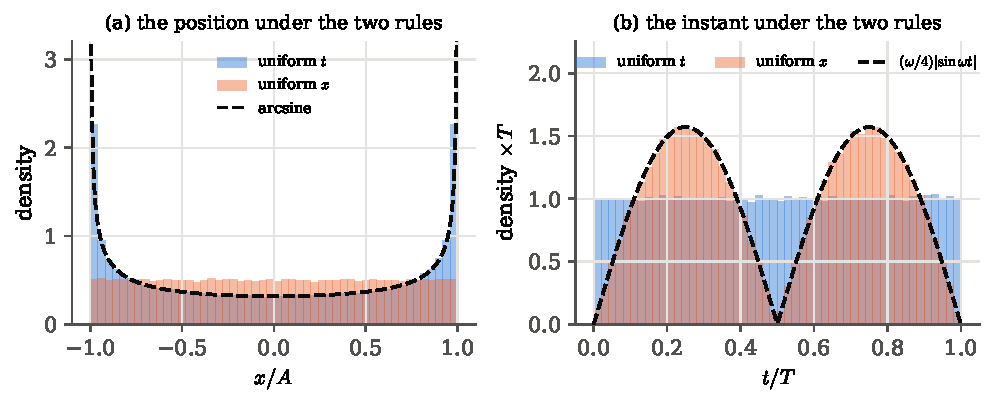
\includegraphics[width=\linewidth]{figures/ch01/oscillator_sampling_rule.pdf}
\caption{One oscillator, two sampling rules, $2\times10^5$ samples each. (a) Choosing
the instant uniformly gives the arcsine law for the position (blue); choosing the
position uniformly gives, by construction, a flat histogram (orange). (b) The
instants behind the same samples: flat under the first rule, and under the second
rule the two humps of $(\omega/4)\abs{\sin\omega t}$, highest where the mass passes
the centre and zero at the turning points $t=0,\,T/2,\,T$.}
\label{1b:fig:sampling-rule}
\end{figure}

\begin{keyidea}[Equations of motion + sampling prescription $\to$ probability distribution]
A deterministic motion has no distribution until we say what is chosen at random.
The same orbit gives the arcsine law for $x$ if the instant is uniform, and
$(\omega/4)\abs{\sin\omega t}$ for $t$ if the position is uniform. Conservation laws
tell us which states are \emph{accessible} (energy conservation confines the
oscillator to its ellipse), not that they are equally probable. Being canonically
conjugate does not make a variable uniform either: the phase $\theta=\omega t$,
conjugate to the action $E/\omega$, is uniform under the first rule only because
that rule chose the instant uniformly, and under the second rule it has density
$\frac14\abs{\sin\theta}$.
\end{keyidea}

\paragraph{Method 3: from first principles, if we did not know that $t$ is uniform.}
Method 2 assumed \eqref{1b:eq:uniform-time}. Suppose we did not know that the
instant is uniformly distributed, and asked instead what statistical mechanics
says: in the \newterm{microcanonical ensemble} all phase-space points with
energy between $E$ and $E+\Delta E$ are equally probable. We then only have to
measure areas in phase space. The energy is
\begin{equation*}
  H(x,p)=\frac{p^2}{2m}+\frac12m\omega^2x^2=E,
  \qquad E=\frac12m\omega^2A^2,
\end{equation*}
so the orbit is the ellipse $x^2/A^2+p^2/(m\omega A)^2=1$, with the two branches
$p_\pm(x)=\pm m\omega\sqrt{A^2-x^2}$. Thicken it into a shell
$E\to E+\Delta E$. At fixed $x$ the shell has thickness in the $p$ direction
\begin{align*}
  \Delta p
  &\eqby{1} \sqrt{2m(E+\Delta E)-m^2\omega^2x^2}-\sqrt{2mE-m^2\omega^2x^2}
   \eqby{2} \frac{m\,\Delta E}{\sqrt{2mE-m^2\omega^2x^2}}
   \eqby{3} \frac{\Delta E}{\omega\sqrt{A^2-x^2}} .
\end{align*}
\begin{explain}
  \item Solve $H=E$ for $\abs p$: $\abs p=\sqrt{2mE-m^2\omega^2x^2}$, at the outer
        and inner energies.
  \item First order in $\Delta E$: $\sqrt{a+\epsilon}-\sqrt a\simeq\epsilon/(2\sqrt a)$
        with $\epsilon=2m\Delta E$.
  \item $2mE=m^2\omega^2A^2$, so the square root is $m\omega\sqrt{A^2-x^2}$.
\end{explain}
The vertical strip between $x$ and $x+\dd x$ meets the shell twice, at $p_+$ and
at $p_-$ (the two dark patches in \cref{1b:fig:arcsine}b), so the shell area
inside the strip and the total shell area are
\begin{align*}
  \dd\mathcal A
  &\eqby{1} 2\,\Delta p\,\dd x
   = \frac{2\Delta E}{\omega\sqrt{A^2-x^2}}\,\dd x,
  \\
  \mathcal A_{\rm shell}
  &\eqby{2} \mathcal A(E+\Delta E)-\mathcal A(E)
   \eqby{3} \frac{2\pi}{\omega}\,\Delta E .
\end{align*}
\begin{explain}
  \item Two patches, each of height $\Delta p$ and width $\dd x$.
  \item The shell is the region between the two ellipses.
  \item The ellipse of energy $E$ has semi-axes $\sqrt{2E/m\omega^2}$ and $\sqrt{2mE}$,
        so it encloses $\mathcal A(E)=\pi\sqrt{2E/m\omega^2}\sqrt{2mE}=2\pi E/\omega$,
        which is linear in $E$.
\end{explain}
Equal probability for equal phase-space area then gives
\begin{align*}
  P(x)\,\dd x
  &\eqby{1} \frac{\dd\mathcal A}{\mathcal A_{\rm shell}}
   \eqby{2} \frac{2\Delta E\,\dd x/\bigl(\omega\sqrt{A^2-x^2}\bigr)}{2\pi\Delta E/\omega}
   = \frac{\dd x}{\pi\sqrt{A^2-x^2}},
  \qquad \abs{x}<A,
\end{align*}
\begin{explain}
  \item Microcanonical ensemble: probability is proportional to phase-space area within the shell.
  \item The two results above; $\Delta E$ and $\omega$ cancel.
\end{explain}
and it is normalised, $\frac1\pi\int_{-A}^{A}\dd x/\sqrt{A^2-x^2}=\frac1\pi[\arcsin(x/A)]_{-A}^{A}=1$.

All three methods agree, and the agreement is not a coincidence. Methods 2 and 3
say the same thing from two ends: the \emph{time} average over one orbit equals
the \emph{ensemble} average over the energy shell. Why? The time spent in a
patch of the shell is its width over the speed, $\dd x/\abs v$. The patch area
is $2\Delta p\,\dd x$, and $\Delta p\propto1/\abs{v}$, so the area is
proportional to the same thing. A uniformly random instant therefore lands in
each patch in proportion to its area. This equality of time and
ensemble averages is \newterm{ergodicity}, and it is the property that makes
Markov-chain sampling work in \cref{ch:09}.

The density diverges at the turning points, where $v=0$, but integrably. For example
\begin{align*}
  \Prob\bigl(\abs X>0.9A\bigr)
  &\eqby{1} 1-\bigl[F_X(0.9A)-F_X(-0.9A)\bigr]
   \eqby{2} 1-\frac2\pi\arcsin0.9
   = 0.2871 ,
\end{align*}
\begin{explain}
  \item Complement of $-0.9A<X\le0.9A$, and \eqref{1b:eq:cdf-rules}.
  \item $\arcsin$ is odd, so $F(0.9A)-F(-0.9A)=\tfrac2\pi\arcsin0.9$.
\end{explain}
so more than a quarter of the time is spent in the outer 10\% of the range, both sides
combined. Averaging $x^2$ over this density gives
$\langle x^2\rangle=A^2/2$ (\cref{1b:sec:expectation}), the statement that the
time-averaged potential energy is half the total.

\pyfile[firstline=23,lastline=28,firstnumber=23]{code/ch01/14_oscillator_arcsine.py}{The oscillator: random instants, deterministic map onto the phase-space orbit}

Line 26 is the only random line: \emph{when} we look. Lines 27--28 apply the
deterministic map to a point $(x,p)$ of the orbit, which is the sampled element of the sample space. Everything else is comparison. The script also computes
the quantum probability density $\abs{\psi_{30}(x)}^2$ of the oscillator
eigenstate with $n=30$, using the stable recursion for Hermite functions
(lines 39--46), at the same energy $E=(n+\tfrac12)\hbar\omega=\tfrac12m\omega^2A^2$,
i.e.\ $A=\sqrt{2n+1}$ in units $\hbar=m=\omega=1$.

\begin{figure}[htbp]
\centering
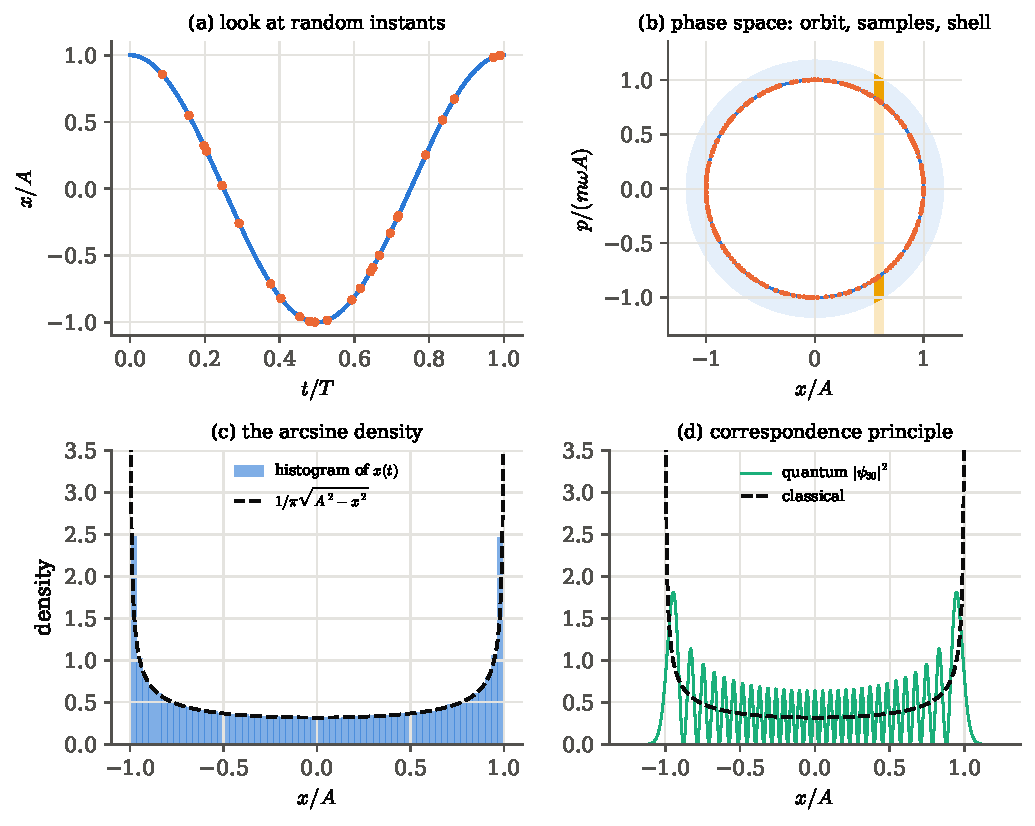
\includegraphics[width=\linewidth]{figures/ch01/oscillator_arcsine.pdf}
\caption{(a) The trajectory, looked at in random instants (dots). (b) The same
instants as points $(x,p)$ of phase space: they all lie on the energy ellipse
(a circle in the scaled units), the sample space of this problem. The pale ring is
a thickened energy shell; the vertical strip between $x$ and $x+\dd x$ meets it in
two dark patches, at $p_+$ and $p_-$, whose area is what Method~3 computes.
(c) The histogram of $x$ at $2\times10^5$ random instants follows the arcsine
density, lowest at the centre and rising steeply towards the turning points.
(d) The quantum density for $n=30$ oscillates rapidly, but its local average
follows the same classical curve: the correspondence principle seen as a
statement about probability densities.}
\label{1b:fig:arcsine}
\end{figure}

The script finds $\Prob(\abs X>0.9A)=\OneBOscFracSim$ (exact
$\OneBOscFracExact$), $\langle x^2\rangle=\OneBOscMeanSq\,A^2$ (exact $0.5$),
and a $\chi^2$ of $\OneBOscChi$ over $\OneBOscNbins$ bins against the
bin-integrated arcsine law, computed from CDF differences (lines 105--109 of
the script).

\paragraph{How research uses it.} The oscillator experiment is: pick random $t$, compute $x(t)$, histogram.
The histogram converges to the density of $x$ without our ever writing
that density down. \Cref{ch:05,ch:09} do exactly this with a posterior: an
MCMC sampler produces points $\params^{(1)},\params^{(2)},\dots$ and the
histogram of any function $g(\params)$ of them (a derived parameter such as
$H_0$ computed from $\Omega_mh^2$ and $\Omega_m$) is its posterior density,
Jacobian included automatically. Here the Monte Carlo \emph{verifies} a
known arcsine law. There it \emph{is} the answer, because the posterior
density of a derived parameter has no closed form.

\subsection{Why every point of the energy shell is equally likely: maximum entropy}
\label{1b:sec:maxent}

Method~3 for the oscillator (\cref{1b:ex:arcsine}) found the arcsine law without
ever mentioning time. It used one sentence instead: all points of the energy shell
are equally probable. Where does that sentence come from? Not from energy
conservation, which only confines the oscillator to its ellipse and says nothing
about how probable each point of it is (the key idea of \cref{1b:ex:arcsine}). It is
an extra assumption, and it can be derived from a cleaner one. Three
assumptions are needed.
\begin{enumerate}[leftmargin=1.6em,itemsep=1pt]
  \item \emph{A probabilistic description.} Cut phase space into small cells
        $i=1,2,\dots$ of equal area $\dd x\,\dd p$. The state of the system is
        described by probabilities $p_i\ge0$ with $\sum_ip_i=1$. Equal area is the
        natural cell size because phase-space area is what the Hamiltonian motion
        preserves (Liouville's theorem).
  \item \emph{Constraints.} What we know about the system is written as equations
        the $p_i$ must obey.
  \item \emph{Equilibrium.} Among all distributions that obey the constraints, the
        equilibrium one maximises the Gibbs--Shannon entropy
        \begin{equation}
          S[p]=-k_B\sum_ip_i\ln p_i .
          \label{1b:eq:gibbs-entropy}
        \end{equation}
\end{enumerate}

\paragraph{Only normalisation: the microcanonical distribution.}
Keep only the $M$ cells of the shell between $E$ and $E+\Delta E$, the accessible
states, and impose nothing but normalisation. With a Lagrange multiplier $k_B\alpha$
for $\sum_ip_i=1$, the maximum has
\begin{align*}
  0
  &\eqby{1}\frac{\partial}{\partial p_j}\Bigl[-k_B\sum_ip_i\ln p_i
       -k_B\alpha\Bigl(\sum_ip_i-1\Bigr)\Bigr]
   \eqby{2}-k_B\bigl(\ln p_j+1+\alpha\bigr),
  \\
  p_j
  &\eqby{3}e^{-1-\alpha}
   \eqby{4}\frac1M\qquad\text{for every cell } j \text{ of the shell}.
\end{align*}
\begin{explain}
  \item The stationary point of the entropy with the constraint added through its
        multiplier.
  \item Only the term $i=j$ depends on $p_j$, and $\frac{\dd}{\dd p}(p\ln p)=\ln p+1$.
  \item Solve for $p_j$.
  \item The right side of (3) is the same number for every $j$; normalisation over
        the $M$ cells fixes it to $1/M$.
\end{explain}
It is a maximum, because $\partial^2S/\partial p_j^2=-k_B/p_j<0$, and its value is
$S=k_B\ln M$, Boltzmann's entropy of \cref{1a:sec:counting}. Equal probability per
cell of equal area means probability proportional to phase-space area: Method~3's
``equal probability for equal phase-space area'' was this assumption.

\paragraph{Normalisation and a fixed mean energy: the canonical distribution.}
Now let the system exchange energy with its surroundings, so that cells of every
energy $E_i$ are accessible, and suppose all we know is the mean energy,
$\sum_ip_iE_i=U$. A second multiplier $\lambda$ enters:
\begin{align*}
  0
  &\eqby{1}\frac{\partial}{\partial p_j}\Bigl[S[p]-k_B\alpha\Bigl(\sum_ip_i-1\Bigr)
        -\lambda\Bigl(\sum_ip_iE_i-U\Bigr)\Bigr]
   \eqby{2}-k_B\bigl(\ln p_j+1+\alpha\bigr)-\lambda E_j,
  \\
  p_j
  &\eqby{3}e^{-1-\alpha}\,e^{-\beta E_j}
   \eqby{4}\frac{e^{-\beta E_j}}{Z},
  \qquad \beta\equiv\frac{\lambda}{k_B},\quad Z=\sum_ie^{-\beta E_i}.
\end{align*}
\begin{explain}
  \item The stationary point with both constraints.
  \item As before, plus $\partial(\sum_ip_iE_i)/\partial p_j=E_j$.
  \item Solve for $\ln p_j$ and exponentiate.
  \item Normalisation fixes $e^{-1-\alpha}=1/Z$; $Z$, the \newterm{partition
        function}, is simply the normaliser.
\end{explain}
What is $\beta$? Put the solution back into the entropy and ask how the maximum
entropy changes with $U$:
\begin{align*}
  S
  &\eqby{1}-k_B\sum_ip_i\bigl(-\beta E_i-\ln Z\bigr)
   \eqby{2}k_B\bigl(\beta U+\ln Z\bigr),
  \\
  \frac{\dd S}{\dd U}
  &\eqby{3}k_B\Bigl(\beta+U\frac{\dd\beta}{\dd U}
        +\frac{\partial\ln Z}{\partial\beta}\frac{\dd\beta}{\dd U}\Bigr)
   \eqby{4}k_B\beta .
\end{align*}
\begin{explain}
  \item $\ln p_i=-\beta E_i-\ln Z$.
  \item $\sum_ip_iE_i=U$ and $\sum_ip_i=1$.
  \item $\beta$ depends on $U$ through the constraint; differentiate both terms.
  \item $\partial_\beta\ln Z=-\sum_iE_ie^{-\beta E_i}/Z=-U$, so the last two terms
        cancel.
\end{explain}
Thermodynamics defines the temperature by $1/T=\dd S/\dd U$. So $\lambda=k_B\beta=1/T$,
that is $\beta=1/k_BT$, and the maximum-entropy distribution at fixed mean energy is
the Boltzmann distribution $p_i=e^{-E_i/k_BT}/Z$.

\paragraph{No sampling rule, and a definition that closes on itself.}
In \cref{1b:ex:arcsine} a probability needed a sampling prescription: choose the
instant, or choose the position, and the answers differed. Here we never said what
is chosen at random, and we did not need to. Why not? The entropy
\eqref{1b:eq:gibbs-entropy} is a function of the probabilities themselves, so
maximising it is a statement about the $p_i$ directly. The third assumption
takes the place of the sampling rule. That assumption is also a definition:
equilibrium \emph{is} the maximum-entropy state compatible with the
constraints. So the argument closes on itself. The microcanonical and
canonical distributions apply exactly when the system is in that state, and
the derivation says nothing about whether, or how fast, a given system gets
there. For the one-dimensional oscillator the dynamics answer that question
at once: a uniform instant lands on the shell in proportion to area (the
ergodicity paragraph of \cref{1b:ex:arcsine}). The same variational argument with a fixed variance gives
the Gaussian as the maximum-entropy density, in \cref{ch:02}.

\subsection{Time averages of a bounded motion: the virial theorem}
\label{1b:sec:virial}

The oscillator's $\langle x^2\rangle=A^2/2$ of \cref{1b:ex:arcsine} is a time
average: under the uniform-instant rule, averaging over the arcsine density is
averaging over one period. It says that the mean potential energy is
$\langle V\rangle=\frac12m\omega^2\langle x^2\rangle=\frac14m\omega^2A^2=E/2$, so the
mean kinetic energy is $\langle K\rangle=E-\langle V\rangle=E/2$ as well:
$2\langle K\rangle=2\langle V\rangle$. This is the virial theorem for a potential
$V\propto x^2$, and the general version takes three lines.

Take particles with positions $\bm r_a$ and momenta $\bm p_a$, potential
$V(\bm r_1,\bm r_2,\dots)$, and kinetic energy $K=\sum_a\bm p_a^2/2m_a$. Let
$G=\sum_a\bm r_a\cdot\bm p_a$ (for one particle in one dimension, $G=xp$). Then
\begin{align*}
  \frac{\dd G}{\dd t}
  &\eqby{1}\sum_a\dot{\bm r}_a\cdot\bm p_a+\sum_a\bm r_a\cdot\dot{\bm p}_a
   \eqby{2}2K-\sum_a\bm r_a\cdot\nabla_aV,
  \\
  \frac{G(\tau)-G(0)}{\tau}
  &\eqby{3}2\langle K\rangle_\tau-\Bigl\langle\sum_a\bm r_a\cdot\nabla_aV\Bigr\rangle_\tau
   \eqby{4}0\quad\text{in the limit }\tau\to\infty .
\end{align*}
\begin{explain}
  \item Product rule.
  \item $\dot{\bm r}_a=\bm p_a/m_a$, so the first sum is $\sum_a\bm p_a^2/m_a=2K$;
        Newton's law $\dot{\bm p}_a=-\nabla_aV$ in the second.
  \item Average both sides over a time $\tau$, $\langle f\rangle_\tau=\frac1\tau\int_0^\tau f\,\dd t$.
  \item For a bounded motion $G$ stays bounded, so the left side goes to zero as
        $\tau\to\infty$ (for a periodic motion it is exactly zero over one period).
\end{explain}
Hence the time-averaged \newterm{virial theorem}
\begin{equation}
  2\langle K\rangle=\Bigl\langle\sum_a\bm r_a\cdot\nabla_aV\Bigr\rangle
  \qquad\Longrightarrow\qquad
  2\langle K\rangle=n\,\langle V\rangle\quad\text{for } V\propto r^n ,
  \label{1b:eq:virial}
\end{equation}
the second form because a potential homogeneous of degree $n$,
$V(\lambda\bm r_1,\lambda\bm r_2,\dots)=\lambda^nV$, obeys Euler's relation
$\sum_a\bm r_a\cdot\nabla_aV=nV$ (differentiate in $\lambda$ at $\lambda=1$). For the
oscillator $n=2$ and $\langle K\rangle=\langle V\rangle$, as found above.

\paragraph{Gravity: negative heat capacity.}
For self-gravitating masses, $V=-\sum_{a<b}Gm_am_b/\abs{\bm r_a-\bm r_b}$ is homogeneous
of degree $n=-1$. Then
\begin{align*}
  E
  &\eqby{1}\langle K\rangle+\langle V\rangle
   \eqby{2}\langle K\rangle-2\langle K\rangle
   =-\langle K\rangle
   \eqby{3}-\tfrac32Nk_BT,
  \qquad
  \frac{\dd E}{\dd T}=-\tfrac32Nk_B<0 .
\end{align*}
\begin{explain}
  \item $E$ is conserved, so it equals its own time average.
  \item The virial theorem \eqref{1b:eq:virial} with $n=-1$: $\langle V\rangle=-2\langle K\rangle$.
  \item The kinetic-gas definition of temperature for $N$ particles,
        $\langle K\rangle=\frac32Nk_BT$.
\end{explain}
A self-gravitating system has a negative heat capacity: when it loses energy it heats
up. A star radiates, contracts, its potential energy falls by twice the energy lost,
and half of that goes into faster thermal motion. Star clusters behave the same way:
the core loses energy to the halo and gets hotter.

\paragraph{The canonical distribution cannot have $C<0$.}
The canonical distribution of \cref{1b:sec:maxent} fixes the sign of the heat
capacity, so it cannot describe such a system. With $Z(\beta)=\sum_ie^{-\beta E_i}$,
\begin{align*}
  \frac{\partial\ln Z}{\partial\beta}
  &\eqby{1}-\frac{\sum_iE_ie^{-\beta E_i}}{Z}=-\langle E\rangle,
  \qquad
  \frac{\partial^2\ln Z}{\partial\beta^2}
  \eqby{2}\frac{\sum_iE_i^2e^{-\beta E_i}}{Z}-\Bigl(\frac{\sum_iE_ie^{-\beta E_i}}{Z}\Bigr)^2
  =\Var(E),
  \\
  C
  &\eqby{3}\frac{\dd\langle E\rangle}{\dd T}
   \eqby{4}\frac{\dd\beta}{\dd T}\,\frac{\dd\langle E\rangle}{\dd\beta}
   \eqby{5}\Bigl(-\frac1{k_BT^2}\Bigr)\Bigl(-\frac{\partial^2\ln Z}{\partial\beta^2}\Bigr)
   =\frac{\Var(E)}{k_BT^2}\;\ge\;0 .
\end{align*}
\begin{explain}
  \item Differentiate $\ln Z$; the ratio is the canonical average of $E$.
  \item Differentiate once more (quotient rule): $\partial_\beta(Z'/Z)=Z''/Z-(Z'/Z)^2$,
        which is $\langle E^2\rangle-\langle E\rangle^2$ (the generating-function view
        of $\ln Z$ is in \cref{1b:sec:moments}).
  \item The heat capacity is the change of mean energy with temperature.
  \item Chain rule through $\beta=1/k_BT$.
  \item $\dd\beta/\dd T=-1/k_BT^2$ and the two results of the first line.
\end{explain}
A variance is never negative, so a system described by the canonical distribution
has $C\ge0$. A self-gravitating system, with $C<0$, cannot be described by the
canonical distribution, and physically it cannot sit in equilibrium with a heat bath:
if it is a little hotter than the bath it loses energy, gets hotter still, and runs
away. Only the microcanonical description, an isolated system at fixed $E$ with
maximum entropy on its shell, can apply to it. The assumptions of
\cref{1b:sec:maxent} say exactly when each distribution is legitimate: fixed energy
gives the microcanonical, a fixed mean energy (which in practice means contact with
a bath) gives the canonical, and the second needs $C\ge0$ to be consistent.

\subsection{Isotropic decays: flat in \texorpdfstring{$\cos\theta$}{cos theta}, peaked in \texorpdfstring{$p_T$}{pT}}

\oneBEx{Angles and transverse momentum of an isotropic decay}\label{1b:ex:decay}
A particle at rest decays into two daughters, each of momentum $p^*$ in
opposite directions. ``Isotropic'' means the daughter direction is uniform
on the unit sphere: the probability of a patch is its solid angle over
$4\pi$, $\dd\Prob=\dd\Omega/4\pi=\sin\theta\,\dd\theta\,\dd\phi/4\pi$ with
$\theta\in[0,\pi]$ the polar angle to the beam axis $z$. Then:
\begin{align*}
  f(\theta)
  &\eqby{1} \int_0^{2\pi}\frac{\sin\theta}{4\pi}\,\dd\phi
   = \frac{\sin\theta}{2},\qquad
  f_{\cos\theta}(u)\eqby{2}\frac{\sin\theta}{2}\cdot\frac{1}{\sin\theta}
   = \frac12,\quad u\in[-1,1].
\end{align*}
\begin{explain}
  \item The joint density of $(\theta,\phi)$ is $\sin\theta/4\pi$.
        Marginalise the azimuth $\phi$.
  \item $u=\cos\theta$ is decreasing on $[0,\pi]$ with
        $\abs{\dd\theta/\dd u}=1/\sin\theta$. Apply \eqref{1b:eq:jacobian-1d}.
\end{explain}
So $\cos\theta$ is flat, $\theta$ is not (few decays go along the beam,
because the poles have little solid angle), and $p_z=p^*\cos\theta$ is
uniform on $[-p^*,p^*]$. The transverse momentum $p_T=p^*\sin\theta$ is
different: two angles, $\theta$ and $\pi-\theta$, give the same $p_T$. With
$\sin\theta=p_T/p^*$ and $\abs{\cos\theta}=\sqrt{1-p_T^2/p^{*2}}$,
\begin{align*}
  \Bigl\lvert\frac{\dd\theta}{\dd p_T}\Bigr\rvert
  &\eqby{1} \frac{1}{p^*\abs{\cos\theta}}
   = \frac{1}{\sqrt{p^{*2}-p_T^2}},\\
  f(p_T)
  &\eqby{2} 2\times\frac{\sin\theta}{2}\times\frac{1}{\sqrt{p^{*2}-p_T^2}}
   = \frac{p_T}{p^*\sqrt{p^{*2}-p_T^2}},\qquad 0<p_T<p^* .
\end{align*}
\begin{explain}
  \item $\dd p_T/\dd\theta=p^*\cos\theta$.
  \item Two branches ($\theta<\pi/2$ and $\theta>\pi/2$) with the same
        density $\sin\theta/2$ and the same Jacobian.
\end{explain}
The density diverges at $p_T=p^*$, the \newterm{Jacobian peak}: decays near
$\theta=\pi/2$ all pile up at the maximum $p_T$, because $p_T$ is stationary
there. For $W\to e\nu$ with the $W$ at rest, $p^*=m_W/2\approx40\,$GeV, and
the sharp edge of the electron $p_T$ spectrum near 40 GeV is what makes the
$p_T$ distribution sensitive to $m_W$. As a check,
$\Prob(p_T>0.9p^*)=\Prob(\abs{\cos\theta}<\sqrt{1-0.81})=\sqrt{0.19}=0.4359$,
because $\cos\theta$ is uniform.

\pyfile[firstline=22,lastline=30,firstnumber=22]{code/ch01/15_decay_angles.py}{Isotropic directions and the transverse momentum}

Lines 26--27 generate isotropic directions by normalising a vector of three
independent standard Gaussians. This works because the joint density of the
three Gaussians, $(2\pi)^{-3/2}e^{-\abs{\bm v}^2/2}$, depends only on the
length $\abs{\bm v}$, so it is unchanged by rotations and the direction must
be uniform. Lines 28--30 compute the three random variables of the example
from the same simulated directions.

\begin{figure}[htbp]
\centering
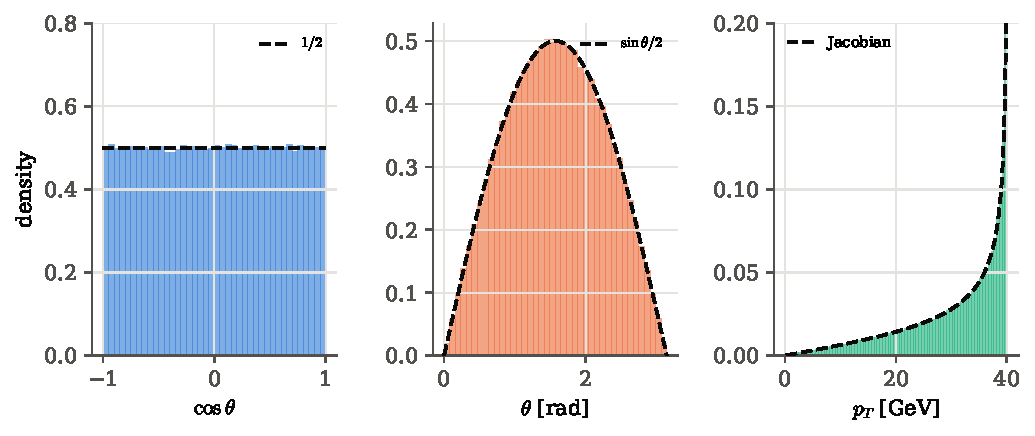
\includegraphics[width=\linewidth]{figures/ch01/decay_angles.pdf}
\caption{$4\times10^5$ isotropic decays of a particle at rest with
$p^*=m_W/2$. Left: $\cos\theta$ is flat at $\tfrac12$. Middle: $\theta$
itself follows $\sin\theta/2$, vanishing along the beam. Right: the
transverse momentum rises towards the kinematic endpoint $p^*$ and piles up
there (the Jacobian peak).}
\label{1b:fig:decay}
\end{figure}

The simulation gives $\langle\cos\theta\rangle=\OneBDecMeanCos$ (exact 0),
$\langle p_T\rangle=\OneBDecMeanPtSim\,$GeV against the exact
$p^*\langle\sin\theta\rangle=\pi p^*/4=\OneBDecMeanPtExact\,$GeV, and
$\Prob(p_T>0.9p^*)=\OneBDecFracSim$ against $\OneBDecFracExact$.

\subsection{Several variables: the Jacobian determinant}

Everything above extends to several variables at once, with lengths replaced
by areas or volumes.

\begin{workdef}[change of variables in several dimensions]
Let $(X,Y)$ have joint density $f_{X,Y}$ and let $(U,V)=g(X,Y)$ be
one-to-one on the region where $f_{X,Y}>0$, with inverse $x=h_1(u,v)$,
$y=h_2(u,v)$. Then
\begin{equation}
  f_{U,V}(u,v)=f_{X,Y}\bigl(h_1(u,v),h_2(u,v)\bigr)\,\abs{J},\qquad
  J=\det\begin{pmatrix}\partial x/\partial u&\partial x/\partial v\\
  \partial y/\partial u&\partial y/\partial v\end{pmatrix},
  \label{1b:eq:jacobian-2d}
\end{equation}
\unpack{the old density at the preimage point, times the factor by which the
inverse map scales areas near it}. The same holds in $n$ dimensions with the
$n\times n$ Jacobian determinant \srcref{Cowan}{(1.37)--(1.38)}.
\emph{Operational test:} a small rectangle $\dd u\,\dd v$ is the image of a
parallelogram of area $\abs J\dd u\,\dd v$, and both must carry the same
probability.
\end{workdef}

The multidimensional formula is \eqref{1b:eq:jacobian-1d} with ``length''
replaced by ``area'': the inverse map sends the rectangle with sides
$\dd u,\dd v$ to a parallelogram spanned by the vectors
$(\partial_ux,\partial_uy)\dd u$ and $(\partial_vx,\partial_vy)\dd v$, whose
area is $\abs{J}\dd u\,\dd v$, the familiar volume element of a coordinate
change.

\oneBEx{Sum and difference of two Gaussians; polar coordinates}\label{1b:ex:sum-diff}
Let $X,Y\iid\Normal(0,1)$ and $U=X+Y$, $V=X-Y$
\srcref{CasellaBerger}{Ex.~4.3.4}. The inverse is $x=(u+v)/2$,
$y=(u-v)/2$, so
\begin{align*}
  J&\eqby{1}\det\begin{pmatrix}\tfrac12&\tfrac12\\ \tfrac12&-\tfrac12\end{pmatrix}=-\tfrac12,
  \qquad x^2+y^2\eqby{2}\frac{(u+v)^2+(u-v)^2}{4}=\frac{u^2+v^2}{2},\\
  f_{U,V}(u,v)
  &\eqby{3} \frac{1}{2\pi}e^{-(u^2+v^2)/4}\cdot\frac12
   = \Bigl[\frac{e^{-u^2/4}}{\sqrt{2\pi\cdot2}}\Bigr]
     \Bigl[\frac{e^{-v^2/4}}{\sqrt{2\pi\cdot2}}\Bigr].
\end{align*}
\begin{explain}
  \item Partial derivatives of $x$ and $y$ with respect to $u,v$.
  \item The cross terms $\pm2uv$ cancel.
  \item \eqref{1b:eq:jacobian-2d} with
        $f_{X,Y}=\tfrac{1}{2\pi}e^{-(x^2+y^2)/2}$ and $\abs J=\tfrac12$.
\end{explain}
The joint factorises: $U$ and $V$ are independent, each $\Normal(0,2)$. The
sum and difference of two equally noisy channels are statistically
independent, a fact \cref{1b:sec:covariance} will explain through their
covariance.

In polar coordinates, $x=r\cos\varphi$, $y=r\sin\varphi$, $J=r$, and the
same density becomes $f(r,\varphi)=\frac{1}{2\pi}\cdot re^{-r^2/2}$: the angle
is uniform on $[0,2\pi)$, independent of the radius, and $R$ has density
$re^{-r^2/2}$ (the Rayleigh distribution). Read backwards this is the
Box--Muller recipe for making Gaussians from uniforms (\cref{ch:06}).

For a single function $Z=r(X,Y)$ the three-step CDF method still works
\mainref{p.~42}: find $A_z=\{(x,y):r(x,y)\le z\}$, integrate the joint over
it, differentiate. Alternatively, invent a second variable to make the map
one-to-one, use \eqref{1b:eq:jacobian-2d}, and marginalise the invented
variable \srcref{CasellaBerger}{\S4.3}. For $Z=X+Y$ take $(x,y)\to(x,z)$ with
$z=x+y$, so $y=z-x$ and $\abs J=1$. For independent $X,Y$ with densities $g,h$:
\begin{align}
  f_Z(z)
  &\eqby{1} \int f_{X,Z}(x,z)\,\dd x
   \eqby{2} \int g(x)\,h(z-x)\,\dd x ,
  \label{1b:eq:convolution}
\end{align}
\begin{explain}
  \item Marginalise the auxiliary variable $x$.
  \item \eqref{1b:eq:jacobian-2d} with $\abs J=1$ and independence,
        $f_{X,Y}(x,z-x)=g(x)h(z-x)$.
\end{explain}
the \newterm{convolution} $g*h$: the density of a sum is the convolution of
the densities \srcref{Cowan}{(1.36)}. For a product $Z=XY$ take $y=z/x$,
$\abs{J}=1/\abs x$, and get $f_Z(z)=\int g(x)h(z/x)\,\dd x/\abs x$, the Mellin
convolution \srcref{Cowan}{(1.35)}.

\oneBEx{The sum of two uniforms is a triangle}\label{1b:ex:triangle}
Let $X_1,X_2\iid\text{Uniform}(0,1)$ and $Y=X_1+X_2$
\mainref{Ex.~2.48, p.~43}. \emph{By geometry}: $A_y=\{x_1+x_2\le y\}$ within
the unit square is a triangle of area $y^2/2$ for $0\le y<1$, and the square
minus a corner triangle of area $(2-y)^2/2$ for $1\le y<2$
(\cref{1b:fig:triangle}). So $F_Y=y^2/2$ and then $1-(2-y)^2/2$, and
$f_Y(y)=y$ on $[0,1]$, $2-y$ on $[1,2]$. \emph{By convolution}
\eqref{1b:eq:convolution}, with $g=h=\mathbb{1}_{[0,1]}$ (the indicator of
$[0,1]$),
\begin{align*}
  f_Y(y)
  &\eqby{1} \int_0^1\mathbb{1}\bigl[0\le y-x\le1\bigr]\,\dd x
   \eqby{2} \min(y,1)-\max(0,y-1)
   = \begin{cases}y,&0\le y\le1,\\ 2-y,&1\le y\le2 .\end{cases}
\end{align*}
\begin{explain}
  \item $g(x)=1$ restricts $x$ to $[0,1]$, and $h(y-x)=1$ needs
        $0\le y-x\le1$.
  \item Both conditions together: $\max(0,y-1)\le x\le\min(1,y)$. The
        integral is the length of that interval.
\end{explain}
Adding two flat distributions gives a peaked one. Adding more gives
something ever closer to a Gaussian, the central limit theorem of
\cref{ch:02}; \cref{1b:sec:moments} shows why the convolution becomes simple
after a Fourier transform.

\begin{figure}[htbp]
\centering
\begin{tikzpicture}[x=2.3cm,y=2.3cm]
  \begin{scope}
    \fill[formblue!30] (0,0) -- (0.65,0) -- (0,0.65) -- cycle;
    \draw (0,0) rectangle (1,1);
    \draw[thick,bdryred] (0.65,0) -- (0,0.65);
    \fill[bdryred] (0.65,0) circle (1.3pt) (0,0.65) circle (1.3pt);
    \node[lbl,anchor=north] at (0.65,-0.02) {$(y,0)$};
    \node[lbl,anchor=east] at (-0.02,0.65) {$(0,y)$};
    \node[lbl,anchor=north] at (0,-0.02) {$0$};
    \node[lbl,anchor=north] at (1,-0.02) {$1$};
    \node[lbl,align=center] at (0.5,-0.5) {$0\le y<1$:\\area $y^2/2$};
  \end{scope}
  \begin{scope}[xshift=3.2cm]
    \fill[formblue!30] (0,0) -- (1,0) -- (1,0.4) -- (0.4,1) -- (0,1) -- cycle;
    \draw (0,0) rectangle (1,1);
    \draw[thick,bdryred] (1,0.4) -- (0.4,1);
    \fill[bdryred] (1,0.4) circle (1.3pt) (0.4,1) circle (1.3pt);
    \node[lbl,anchor=west] at (1.02,0.4) {$(1,y-1)$};
    \node[lbl,anchor=south] at (0.4,1.02) {$(y-1,1)$};
    \node[lbl,anchor=north] at (0,-0.02) {$0$};
    \node[lbl,anchor=north] at (1,-0.02) {$1$};
    \node[lbl,align=center] at (0.5,-0.5) {$1\le y<2$:\\area $1-(2-y)^2/2$};
  \end{scope}
\end{tikzpicture}
\caption{The event $X_1+X_2\le y$ inside the unit square is everything below
the red line $x_2=y-x_1$. For $y<1$ it is a small triangle. For $y>1$ it is
the whole square minus the unshaded corner. The shaded area is the CDF of the
sum.}
\label{1b:fig:triangle}
\end{figure}

The worked cases used every method in turn. The table says which one to
reach for in each situation.

\begin{taxonomy}[Which method for which transformation]
\begin{center}
\small
\begin{tabular}{@{}p{4.3cm}p{8.1cm}@{}}
\toprule
situation & method\\\midrule
$X$ discrete & add probabilities of all preimages\\
$r$ monotone & $f_Y=f_X(s(y))\abs{s'(y)}$\\
$r$ many-to-one (e.g.\ $x^2$, $\cos$, $\sin$) & sum the monotone formula over branches, or use the CDF\\
awkward region, piecewise & CDF method: draw $A_y$, integrate, differentiate\\
$n$ variables to $n$ variables & Jacobian determinant \eqref{1b:eq:jacobian-2d}\\
one function of $n$ variables & add auxiliary variables, Jacobian, marginalise; sums $\to$ convolution\\
sums of many independent variables & characteristic functions (\cref{1b:sec:moments})\\
anything else & simulate and histogram (Monte Carlo, \cref{ch:06})\\
\bottomrule
\end{tabular}
\end{center}
\end{taxonomy}

Three mistakes recur in all of these methods.

\begin{pitfall}[Transforming the density's value instead of its argument]
Writing $f_Y(y)=f_X(s(y))$ and forgetting the Jacobian is the commonest
error. The result is not normalised, so a quick check $\int f_Y=1$ catches
it. A second error is forgetting branches ($\theta$ and $\pi-\theta$ both give
the same $p_T$). A third is expecting the peak to transform like a point:
modes move under reparametrisation, quantiles do not
(\cref{1b:ex:log-exp}).
\end{pitfall}
\section{Expectation and variance: the long-run average and the spread}
\label{1b:sec:expectation}

A slot machine pays \$100 with probability $0.001$, pays \$5 with probability
$0.14$, and otherwise takes our \$1. Should we play? No single pull answers
that, because a single pull is random. What we can predict is the average
over many pulls. In $N$ pulls we expect about $0.001N$ big wins, $0.14N$
small wins and $0.859N$ losses, so the average payoff per pull is
\[
  0.001\times100+0.14\times5+0.859\times(-1)=-0.059
\]
dollars. In the long run we lose about six cents per pull
\srcref{Kruschke}{\S4.3.3}. Each possible value was weighted by how often it
occurs. That weighted average is the expectation.

Physicists use this object all the time under other names. The ensemble
average $\langle A\rangle=\sum_ip_iA_i$ of statistical mechanics, with
$p_i=e^{-\beta E_i}/Z$, is an expectation. So is the quantum expectation value
$\langle\psi\rvert\hat A\lvert\psi\rangle=\sum_a a\,\abs{\langle a\vert\psi\rangle}^2$,
where the Born probabilities $\abs{\langle a\vert\psi\rangle}^2$ weight the
eigenvalues $a$. Two numbers summarise a whole distribution: a location (the
mean) and a spread (the variance). There are rules for computing both for
sums, for functions and for conditional situations, without ever writing down
the density of the quantity being averaged. Three questions organise the
topic.
\begin{enumerate}[leftmargin=1.6em,itemsep=1pt]
  \item What is the average value of $X$, and of any function $r(X)$?
  \item How far from that average does $X$ typically fall?
  \item If we learn the value of another variable, how do the average and the
        spread change, and how do the conditional pieces reassemble into the
        whole?
\end{enumerate}

\subsection{The expectation}

Start from data. Draw $X$ independently $N$ times and let $n_x$ be the number
of draws that gave the value $x$. The average of the draws is
\[
  \frac1N\sum_{j=1}^NX_j=\sum_x x\,\frac{n_x}{N} .
\]
The frequencies $n_x/N$ approach the probabilities $f(x)=\Prob(X=x)$ as $N$
grows (the frequency interpretation of \cref{1a:sec:axioms}; the law of large
numbers in \cref{ch:02} makes this precise). So the long-run average is
$\sum_x x\,f(x)$. For a continuous variable, sort the draws into bins of
width $\Delta x$. The fraction in the bin at $x$ is about $f(x)\,\Delta x$,
where $f$ is the density, and the sum over bins becomes an integral as
$\Delta x\to0$.

\begin{workdef}[expectation, mean]
The \newterm{expectation} (or \newterm{mean}, or first moment) of $X$ is
\begin{equation}
  \E(X)=\begin{cases}
    \sum_x x\,f(x) & X\text{ discrete},\\[3pt]
    \int_{-\infty}^{\infty}x\,f(x)\,\dd x & X\text{ continuous},
  \end{cases}
  \label{1b:eq:mean}
\end{equation}
the values weighted by the pmf \unpack{$f(x)=\Prob(X=x)$, the mass at $x$} or
by the density \unpack{probability per unit $x$}.
It is written $\mu$, $\mu_X$, $\E X$ or $\langle X\rangle$ and has the units of
$X$. It \newterm{exists} only if $\sum_x\abs x f(x)$ (or
$\int\abs x f(x)\,\dd x$) is finite.
\emph{Operational test:} the average of many independent draws of $X$ settles
down to $\E(X)$.
\end{workdef}

\mainref{Def.~3.1, p.~47} writes both cases as $\int x\,\dd F(x)$, a single
notation for ``sum against the masses or integrate against the density''.
We will use the two explicit forms.

\paragraph{Example: simple means.}
For a Bernoulli trial, $\E(X)=0\cdot(1-p)+1\cdot p=p$: the mean of an
indicator is the probability of the event it indicates. For the number of
heads in two fair flips, $\E(X)=0\cdot\tfrac14+1\cdot\tfrac12+2\cdot\tfrac14=1$
\mainref{Exs.~3.2--3.3, p.~48}. For a fair die,
$\E(X)=\tfrac16(1+2+\dots+6)=\tfrac{21}{6}=3.5$ \srcref{SeeingTheory}{p.~10},
a value the die can never show. The mean is a long-run average, not a
typical outcome. For $X\sim\mathrm{Uniform}(-1,3)$ the density is $\tfrac14$
on $(-1,3)$ and
\begin{align*}
  \E(X)
  &\eqby{1} \int_{-1}^{3}x\cdot\tfrac14\,\dd x
   \eqby{2} \tfrac14\Bigl[\tfrac{x^2}{2}\Bigr]_{-1}^{3}
   = \tfrac14\cdot\tfrac{9-1}{2}=1 .
\end{align*}
\begin{explain}
  \item \eqref{1b:eq:mean} with $f=\tfrac14$ inside the interval and $0$ outside.
  \item Antiderivative of $x$.
\end{explain}
The mean is the midpoint, as symmetry demands. The same happens for the
parabola $f(x)=6x(1-x)$ on $[0,1]$ \srcref{Kruschke}{(4.7)}:
$\E(X)=6\int_0^1(x^2-x^3)\,\dd x=6\bigl(\tfrac13-\tfrac14\bigr)=\tfrac12$.

\paragraph{Example: the mean lifetime.}
A lifetime with density $f(x)=e^{-x/\beta}/\beta$ for $x>0$
(exponential with mean $\beta$, \cref{1b:sec:pdf}) has
\begin{align*}
  \E(X)
  &\eqby{1} \int_0^\infty x\,\frac{e^{-x/\beta}}{\beta}\,\dd x
   \eqby{2} \beta\int_0^\infty u\,e^{-u}\,\dd u \\
  &\eqby{3} \beta\Bigl(\bigl[-u\,e^{-u}\bigr]_0^\infty+\int_0^\infty e^{-u}\,\dd u\Bigr)
   \eqby{4} \beta\,(0+1)=\beta .
\end{align*}
\begin{explain}
  \item Definition \eqref{1b:eq:mean}; the density vanishes for $x<0$.
  \item Substitute $u=x/\beta$, so $x=\beta u$ and $\dd x=\beta\,\dd u$.
  \item Integrate by parts with $u$ differentiated and $e^{-u}$ integrated.
  \item $ue^{-u}\to0$ at both ends, and $\int_0^\infty e^{-u}\dd u=1$.
\end{explain}
So $\beta$ really is the mean lifetime, and the median $\beta\ln2$ found in
\cref{1b:ex:exp-quantile} sits below it.

\paragraph{The balance point.}
If we read $f(x)$ as a mass density along a rod (or as point masses $f(x_i)$
at positions $x_i$), then $\E(X)=\sum_ix_if(x_i)$ with $\sum_if(x_i)=1$ is the
centre of mass: the rod balances on a fulcrum placed at the mean
(\cref{1b:fig:balance}). A small mass far out in a tail pulls the balance
point a long way. This is why the mean of a skewed distribution is dragged
towards its long tail, and why a single outlier can move a sample mean a lot.

\begin{figure}[htbp]
\centering
\begin{tikzpicture}[x=2.0cm,y=4.0cm]
  \draw[thick] (-0.4,0) -- (4.4,0);
  \foreach \k/\p in {0/0.2401,1/0.4116,2/0.2646,3/0.0756,4/0.0081}{
    \fill[formblue!55] ({\k-0.18},0.02) rectangle ({\k+0.18},{0.02+\p});
    \node[lbl,anchor=north] at (\k,-0.17) {$\k$};
    \node[lbl,anchor=south] at (\k,{0.02+\p}) {$\p$};
  }
  \fill[bdryred] (1.2,0) -- (1.08,-0.16) -- (1.32,-0.16) -- cycle;
  \node[lbl,anchor=west,bdryred] at (1.4,-0.08) {$\E(X)=np=1.2$};
  \node[lbl,anchor=north] at (2,-0.34) {number of successes $x$};
\end{tikzpicture}
\caption{The pmf of a binomial with $n=4$, $p=0.3$, drawn as masses on a rod.
The rod balances on the red fulcrum at $x=1.2$, which is the mean. The mean is
not one of the possible values, and it lies to the right of the most probable
value $x=1$ because the tail extends to the right.}
\label{1b:fig:balance}
\end{figure}

\paragraph{Example: a density with no mean.}
The Cauchy density $f(x)=1/[\pi(1+x^2)]$ is the Breit--Wigner (Lorentzian)
line shape of a resonance with unit half-width, centred at $0$. It is
symmetric, so one is tempted to say its mean is $0$. But the mean exists only
if $\int\abs x f(x)\,\dd x$ is finite, and
\begin{align*}
  \int_{-\infty}^{\infty}\frac{\abs x}{\pi(1+x^2)}\,\dd x
  &\eqby{1} \frac2\pi\int_0^\infty\frac{x}{1+x^2}\,\dd x
   \eqby{2} \frac1\pi\Bigl[\ln(1+x^2)\Bigr]_0^\infty=\infty .
\end{align*}
\begin{explain}
  \item The integrand is even, so the integral is twice the integral over $x>0$.
  \item $\frac{\dd}{\dd x}\ln(1+x^2)=\frac{2x}{1+x^2}$, and the logarithm grows
        without bound.
\end{explain}
(\mainref{Ex.~3.5, p.~48} reaches the same conclusion by parts.) The tails
fall only like $1/x^2$, so $x f(x)\sim1/(\pi x)$ and the integral diverges
logarithmically. The positive and negative halves are each infinite, and
``$\infty-\infty$'' has no value. This is not a mathematical curiosity. In a
simulation the running average never settles down: every so often a draw
from far out in a tail arrives and moves the average by a finite amount,
however many draws came before (\cref{1b:fig:cauchy-run}, the computer
experiment of \mainref{Exercise~3.9, p.~59}). After $\OneBRunN$ draws the four
Gaussian averages are all within $\OneBRunGaussMax$ of zero, while the four
Cauchy averages lie between $\OneBRunCauchyMin$ and $\OneBRunCauchyMax$ in
absolute value and are still jumping. \Cref{1b:sec:moments} will show the
reason: the average of $n$ Cauchy draws has exactly the same Cauchy
distribution as a single draw.

\begin{figure}[htbp]
\centering
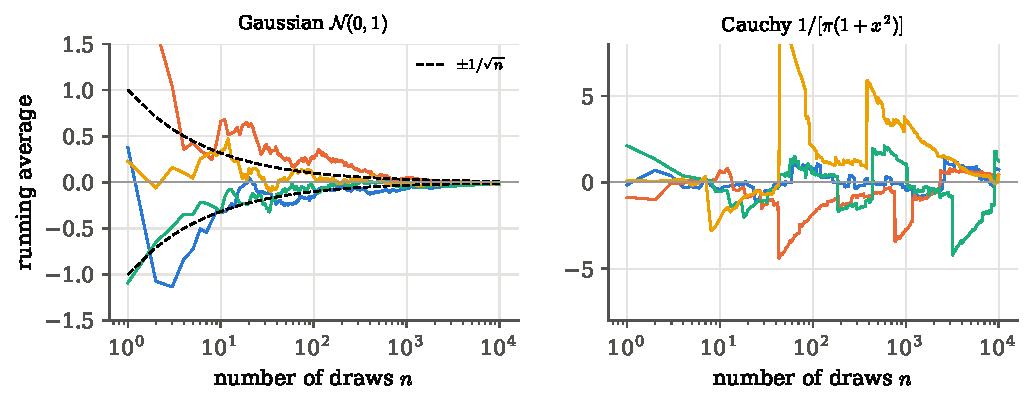
\includegraphics[width=\linewidth]{figures/ch01/cauchy_running_mean.pdf}
\caption{Running averages of four independent sequences of draws, on a
logarithmic axis in $n$. Left: Gaussian draws; the averages close in on zero
inside the dashed $\pm1/\sqrt n$ envelope. Right: Cauchy draws; the averages
wander and jump whenever a very large draw arrives, and do not converge.}
\label{1b:fig:cauchy-run}
\end{figure}

From here on, whenever we write an expectation we assume it exists.

\subsection{The average of a function: the lazy statistician}

Often we want the mean of $Y=r(X)$: the kinetic energy $\tfrac12mv^2$ of a
molecule with random velocity, the flux $10^{-0.4m}$ of a star of random
magnitude, the $p_T$ of a decay product at a random angle. One route is to
find $f_Y$ by the change-of-variables rules of \cref{1b:sec:transform} and
average $y$ against it. There is a much easier way
\mainref{Thm.~3.6, p.~48}:
\begin{equation}
  \E\bigl(r(X)\bigr)=\sum_xr(x)\,f_X(x)
  \quad\text{or}\quad
  \E\bigl(r(X)\bigr)=\int r(x)\,f_X(x)\,\dd x .
  \label{1b:eq:lotus}
\end{equation}
It is called the rule of the lazy statistician because it looks like what a
lazy person would write without thinking, and it is right. Think of a game
in which $X$ is drawn and we are paid $r(X)$: our average income is each
payment $r(x)$ times the chance of that $x$, summed.

Why does it hold? For discrete $X$ \mainref{Exercise~3.6, p.~59}, group the
values of $x$ according to the value $y=r(x)$ they produce:
\begin{align*}
  \E(Y)
  &\eqby{1} \sum_y y\,\Prob(Y=y)
   \eqby{2} \sum_y y\sum_{x:\,r(x)=y}f_X(x)
   \eqby{3} \sum_y\ \sum_{x:\,r(x)=y}r(x)\,f_X(x)
   \eqby{4} \sum_x r(x)\,f_X(x) .
\end{align*}
\begin{explain}
  \item Definition \eqref{1b:eq:mean} applied to $Y$.
  \item $\Prob(Y=y)$ is the total mass of all preimages of $y$
        (\cref{1b:sec:transform}).
  \item Inside the inner sum $r(x)=y$, so $y$ may be replaced by $r(x)$.
  \item Every $x$ lies in exactly one set $\{x:r(x)=y\}$, so the double sum
        visits each $x$ once.
\end{explain}
For continuous $X$ and increasing $r$ with inverse $s$, the same thing
happens with a Jacobian:
\begin{align*}
  \E(Y)
  &\eqby{1} \int y\,f_X\bigl(s(y)\bigr)\,s'(y)\,\dd y
   \eqby{2} \int r(x)\,f_X(x)\,\dd x .
\end{align*}
\begin{explain}
  \item Definition of $\E(Y)$ with $f_Y$ from \eqref{1b:eq:jacobian-1d}.
  \item Substitute $x=s(y)$, so $y=r(x)$ and $\dd x=s'(y)\,\dd y$.
\end{explain}
The Jacobian in the density is exactly cancelled by the Jacobian of the
measure. In the fluid picture: $f_Y(y)\,\dd y=f_X(x)\,\dd x$ is the same
drop of probability, and we multiply it by the same number $y=r(x)$
whichever coordinate we use \srcref{Cowan}{(1.40)}. A decreasing $r$ or
several branches give the same result branch by branch.

The most important special case is an indicator. Let $r=I_A$, the indicator
of a set $A$ ($I_A(x)=1$ if $x\in A$ and $0$ otherwise). Then
\begin{equation}
  \E\bigl(I_A(X)\bigr)=\int I_A(x)f_X(x)\,\dd x=\int_Af_X(x)\,\dd x=\Prob(X\in A).
  \label{1b:eq:prob-as-mean}
\end{equation}
Probability is a special case of expectation. This is how every Monte Carlo
estimate of a probability works (\cref{ch:06}): the fraction of simulated
draws that land in $A$ is the sample mean of an indicator.

\paragraph{Example: $\E(e^X)$ two ways.}
Let $X\sim\mathrm{Uniform}(0,1)$ and $Y=e^X$ \mainref{Ex.~3.7, p.~49}.
By \eqref{1b:eq:lotus}, $\E(Y)=\int_0^1e^x\,\dd x=e-1$. The long way first
finds $f_Y$: the inverse is $s(y)=\ln y$ with $s'(y)=1/y$, so
\eqref{1b:eq:jacobian-1d} gives $f_Y(y)=1/y$ on $(1,e)$, and
$\E(Y)=\int_1^e y\cdot\tfrac1y\,\dd y=e-1$. Same answer, more work. A
simulation with $10^6$ draws gives $\OneBExpUSim$ (exact $\OneBExpUExact$).
Note that $e^{\E(X)}=e^{1/2}=1.649$ is \emph{not} the answer.

\paragraph{Example: the broken stick.}
Break a stick of unit length at a uniformly random point $X$ and keep the
longer piece, $Y=\max\{X,1-X\}$ \mainref{Ex.~3.8, p.~49}. On $x<\tfrac12$ the
longer piece is $1-x$, on $x\ge\tfrac12$ it is $x$:
\begin{align*}
  \E(Y)
  &\eqby{1} \int_0^{1/2}(1-x)\,\dd x+\int_{1/2}^1x\,\dd x
   \eqby{2} \Bigl(\tfrac12-\tfrac18\Bigr)+\Bigl(\tfrac12-\tfrac18\Bigr)
   =\tfrac34 .
\end{align*}
\begin{explain}
  \item \eqref{1b:eq:lotus} with the density $1$ on $(0,1)$, split where $r$
        changes formula.
  \item $\int_0^{1/2}(1-x)\dd x=\tfrac12-\tfrac18$, and
        $\int_{1/2}^1x\,\dd x=\tfrac12-\tfrac18$.
\end{explain}
The simulation gives $\OneBStickSim$.

\paragraph{Example: time average and ensemble average for the oscillator.}
For the oscillator $x(t)=A\cos\omega t$ of \cref{1b:ex:arcsine} we can compute
$\langle x^2\rangle$ in two ways. As an average over the position density
$f(x)=1/(\pi\sqrt{A^2-x^2})$:
\begin{align*}
  \E(X^2)
  &\eqby{1} \int_{-A}^{A}\frac{x^2}{\pi\sqrt{A^2-x^2}}\,\dd x
   \eqby{2} \frac1\pi\int_{-\pi/2}^{\pi/2}\frac{A^2\sin^2\varphi}{A\cos\varphi}\,A\cos\varphi\,\dd\varphi
   \eqby{3} \frac{A^2}{\pi}\cdot\frac\pi2=\frac{A^2}{2} .
\end{align*}
\begin{explain}
  \item \eqref{1b:eq:lotus} with $r(x)=x^2$.
  \item Substitute $x=A\sin\varphi$: $\dd x=A\cos\varphi\,\dd\varphi$ and
        $\sqrt{A^2-x^2}=A\cos\varphi\ge0$ on $[-\tfrac\pi2,\tfrac\pi2]$.
  \item $\int_{-\pi/2}^{\pi/2}\sin^2\varphi\,\dd\varphi=\tfrac\pi2$ (the average
        of $\sin^2$ over a half period is $\tfrac12$).
\end{explain}
As an average over the uniform time $T$ on one period $P=2\pi/\omega$, again
by \eqref{1b:eq:lotus} but now with $X=r(T)$:
$\E(X^2)=\frac1P\int_0^PA^2\cos^2\omega t\,\dd t=\frac{A^2}{2}$. The ensemble
average over positions equals the time average over one period, a small
instance of the ergodic idea that returns with Markov chains in \cref{ch:09}.
Multiplied by $\tfrac12m\omega^2$ it says that the mean potential energy is half
the total energy. The simulation with $A=1$ gives $\OneBOscMeanSq$.

The rule extends to several variables \mainref{(3.4), p.~49},
\[
  \E\bigl(r(X,Y)\bigr)=\iint r(x,y)\,f(x,y)\,\dd x\,\dd y .
\]
For $(X,Y)$ uniform on the unit square,
$\E(X^2+Y^2)=\int_0^1\!\int_0^1(x^2+y^2)\,\dd x\,\dd y=\tfrac13+\tfrac13=\tfrac23$
\mainref{Ex.~3.9, p.~49}.

\begin{pitfall}[The average of a function is not the function of the average]
In general $\E\bigl(r(X)\bigr)\neq r\bigl(\E X\bigr)$: above,
$\E(e^X)=1.718$ but $e^{\E X}=1.649$. Equality holds for linear $r$ only. For
a convex $r$ (curving upwards, like $x^2$ or $e^x$) the inequality always runs
one way, $\E\,r(X)\ge r(\E X)$ (Jensen's inequality,
\srcref{CasellaBerger}{Thm.~4.7.7}), which is why $\langle v^2\rangle\ge\langle
v\rangle^2$. Averaging magnitudes and then converting to flux, or averaging
$\ln\Like$ and exponentiating, gives biased answers for the same reason.
\end{pitfall}

\subsection{Linearity, and products of independent variables}

The single most useful property of the expectation is that it is linear,
whether or not the variables are independent \mainref{Thm.~3.11, p.~50}. For
two continuous variables with joint density $f(x,y)$:
\begin{align*}
  \E(aX+bY)
  &\eqby{1} \iint(ax+by)\,f(x,y)\,\dd x\,\dd y\\
  &\eqby{2} a\int x\Bigl[\int f(x,y)\,\dd y\Bigr]\dd x
           +b\int y\Bigl[\int f(x,y)\,\dd x\Bigr]\dd y\\
  &\eqby{3} a\int x\,f_X(x)\,\dd x+b\int y\,f_Y(y)\,\dd y
   \eqby{4} a\,\E(X)+b\,\E(Y) .
\end{align*}
\begin{explain}
  \item The lazy statistician for two variables, with $r(x,y)=ax+by$.
  \item Split the integral into two and do the inner integral over the
        variable that does not appear in front.
  \item The inner integrals are the marginal densities (\cref{1b:sec:joint}).
  \item Definition \eqref{1b:eq:mean}.
\end{explain}
No independence was used: marginalisation did all the work. By induction,
$\E\bigl(\sum_ia_iX_i\bigr)=\sum_ia_i\E(X_i)$ for any number of variables, and
$\E(aX+b)=a\E(X)+b$ because a constant is a variable with all its mass at one
point.

\paragraph{Example: the binomial mean by indicators.}
The definition gives $\E(X)=\sum_{x=0}^nx\binom nxp^x(1-p)^{n-x}$, which is
not an inviting sum. Instead write the number of successes as a sum of
indicators, $X=\sum_{i=1}^nX_i$ with $X_i=1$ if trial $i$ succeeds
\mainref{Ex.~3.12, p.~50}. Each $\E(X_i)=p$, so linearity gives
\[
  \E(X)=\sum_{i=1}^n\E(X_i)=np .
\]
This is the exact value $5$ that the simulation of \cref{1b:sec:rv} found as
$\OneBMeanX$ for ten fair flips. Linearity turned a combinatorial sum into one
line. The same trick gives the mean count of any multinomial bin,
$\E(X_j)=np_j$.

\paragraph{Example: the mean of the smeared energy.}
In the detector example of \cref{1b:ex:smearing} the measured energy is
$E_{\rm meas}=E+\eps$, the true energy plus a Gaussian error with mean $0$.
Linearity gives $\E(E_{\rm meas})=\E(E)+\E(\eps)=\beta+0=20\,$GeV without
touching the convolution integral \eqref{1b:eq:smear-integral}. The
simulation found $\OneBSmearMeanSim\,$GeV.

For products the situation is different. If $X$ and $Y$ are independent then
$f(x,y)=f_X(x)f_Y(y)$ and \mainref{Thm.~3.13, p.~50}
\begin{align}
  \E(XY)
  &\eqby{1} \iint xy\,f_X(x)f_Y(y)\,\dd x\,\dd y
   \eqby{2} \Bigl(\int x\,f_X(x)\,\dd x\Bigr)\Bigl(\int y\,f_Y(y)\,\dd y\Bigr)
   = \E(X)\,\E(Y) .
  \label{1b:eq:product-mean}
\end{align}
\begin{explain}
  \item Lazy statistician with $r=xy$, and the factorised joint density.
  \item The integrand is a function of $x$ times a function of $y$, so the
        double integral is a product of single integrals.
\end{explain}
The same argument gives, for any functions $g$ and $h$
\srcref{CasellaBerger}{Thm.~4.2.10},
\[
  \E\bigl(g(X)h(Y)\bigr)=\E\bigl(g(X)\bigr)\,\E\bigl(h(Y)\bigr)
\]
(\srcref{SeeingTheory}{p.~32} gives the discrete version). Without
independence it fails: if $X=Y$ is a fair coin indicator then
$\E(XY)=\E(X^2)=\tfrac12$, while $\E(X)\E(Y)=\tfrac14$.

\begin{keyidea}[What expectation respects]
$\E\bigl(\sum_ia_iX_i+b\bigr)=\sum_ia_i\E(X_i)+b$ always. The mean of a
product is the product of the means when the variables are independent, and
not in general.
\end{keyidea}

\subsection{The mean as the best single guess}

Suppose we must summarise $X$ by one number $b$ and we are penalised by the
squared miss $(X-b)^2$. Which $b$ minimises the expected penalty?
Adding and subtracting $\mu=\E X$ answers it without calculus
\srcref{CasellaBerger}{Ex.~2.2.6}:
\begin{align}
  \E(X-b)^2
  &\eqby{1} \E\bigl[(X-\mu)+(\mu-b)\bigr]^2 \nonumber\\
  &\eqby{2} \E(X-\mu)^2+2(\mu-b)\,\E(X-\mu)+(\mu-b)^2 \nonumber\\
  &\eqby{3} \E(X-\mu)^2+(\mu-b)^2 .
  \label{1b:eq:mse-split}
\end{align}
\begin{explain}
  \item Add and subtract $\mu$ inside the bracket.
  \item Expand the square and use linearity; $\mu-b$ is a constant and comes
        out of the expectation.
  \item $\E(X-\mu)=\E X-\mu=0$.
\end{explain}
The first term does not depend on $b$ and the second is smallest, zero, at
$b=\mu$. So the mean is the best guess under squared loss, and the smallest
achievable expected squared miss is $\E(X-\mu)^2$, which is the variance we
define next \srcref{Kruschke}{\S4.3.3.1}. Equation \eqref{1b:eq:mse-split} is a
Pythagoras theorem: total squared miss = spread about the mean + squared
offset of the guess. It returns in \cref{ch:03} as ``mean squared error =
variance + bias$^2$''.

If the penalty is the absolute miss $\abs{X-M}$, the best guess is the median
instead. Write $\E\abs{X-M}=\int_{-\infty}^M(M-x)f(x)\,\dd x+\int_M^\infty(x-M)f(x)\,\dd x$
and differentiate in $M$:
\begin{align*}
  \frac{\dd}{\dd M}\E\abs{X-M}
  &\eqby{1} \int_{-\infty}^Mf(x)\,\dd x-\int_M^\infty f(x)\,\dd x
   \eqby{2} F(M)-\bigl(1-F(M)\bigr)=2F(M)-1 .
\end{align*}
\begin{explain}
  \item Leibniz rule. The boundary terms vanish because each integrand is zero
        at $x=M$, leaving the derivatives $+1$ and $-1$ of the integrands.
  \item Definition of the CDF $F$ (\cref{1b:sec:pdf}).
\end{explain}
The derivative is negative for $F(M)<\tfrac12$ and positive after, so the
minimum is at $F(M)=\tfrac12$, the median. With a penalty of $0$ for an exact
hit and $1$ for any miss, the best guess is the mode. These three loss
functions reappear in \cref{ch:05}, where they turn a posterior into the
posterior mean, median and mode. \Cref{1b:fig:mean-minimiser} checks the first
two for an exponential with $\beta=1$: the simulated squared loss is smallest
at $M=\OneBArgminSq$ (exact $1$), where it equals $\OneBMinSq$ (the variance,
exact $1$), and the absolute loss is smallest at $M=\OneBArgminAbs$ (exact
$\ln2=0.693$).

\begin{figure}[htbp]
\centering
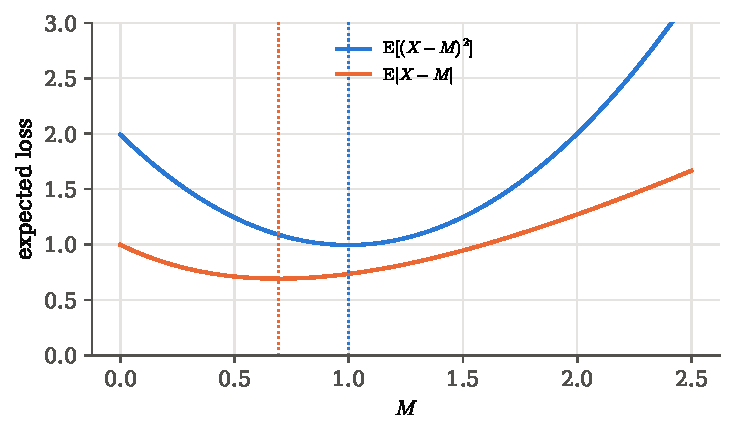
\includegraphics[width=0.72\linewidth]{figures/ch01/mean_minimiser.pdf}
\caption{Expected squared miss and expected absolute miss of a guess $M$ for
exponential lifetimes with mean $1$, computed by averaging over simulated
draws. The squared miss bottoms out at the mean (blue dotted line), the
absolute miss at the median $\ln 2$ (orange dotted line). The height of the
blue minimum is the variance.}
\label{1b:fig:mean-minimiser}
\end{figure}

\subsection{Variance and standard deviation}

The mean says where a distribution sits. We also need how wide it is. The
obvious candidate, the average deviation $\E(X-\mu)$, is useless: it is always
$\E X-\mu=0$, because positive and negative deviations cancel by the definition
of $\mu$ \mainref{p.~50, footnote}. The average absolute deviation
$\E\abs{X-\mu}$ works but is awkward algebraically. The average
\emph{squared} deviation is the standard choice, and
\eqref{1b:eq:mse-split} has already shown why it is natural.

\begin{workdef}[variance, standard deviation]
The \newterm{variance} of $X$ is the mean squared deviation from the mean,
\begin{equation}
  \Var(X)=\sigma^2=\E\bigl[(X-\mu)^2\bigr]
  =\int(x-\mu)^2f(x)\,\dd x ,
  \label{1b:eq:var}
\end{equation}
\unpack{units of $X$ squared}. The \newterm{standard deviation} is
$\sigma=\sqrt{\Var(X)}$ \unpack{same units as $X$, a typical size of
$X-\mu$}.
\emph{Operational test:} the average of $(X_j-\bar X)^2$ over many draws.
\end{workdef}

Three properties do most of the work \mainref{Thm.~3.15, p.~51}.
First, the shortcut formula:
\begin{align}
  \Var(X)
  &\eqby{1} \E\bigl[X^2-2\mu X+\mu^2\bigr]
   \eqby{2} \E(X^2)-2\mu\,\E(X)+\mu^2
   \eqby{3} \E(X^2)-\mu^2 .
  \label{1b:eq:var-short}
\end{align}
\begin{explain}
  \item Expand the square in \eqref{1b:eq:var}.
  \item Linearity; $\mu$ is a constant.
  \item $\E(X)=\mu$, so $-2\mu^2+\mu^2=-\mu^2$.
\end{explain}
Second, shifting does nothing and scaling scales:
$\Var(aX+b)=\E\bigl[(aX+b-a\mu-b)^2\bigr]=a^2\E(X-\mu)^2=a^2\Var(X)$.
Third, $\Var(X)\ge0$, with equality only when $X$ equals a constant with
probability one, since a non-negative quantity $(X-\mu)^2$ can have zero mean
only if it is zero with probability one \mainref{Exercise~3.2, p.~59}.

\paragraph{Example: Bernoulli, die, uniform, exponential.}
For a Bernoulli trial $X^2=X$, so $\E(X^2)=p$ and
$\Var(X)=p-p^2=p(1-p)$, largest for a fair coin and zero when the outcome is
certain. For a fair die
\[
  \Var(X)=\E(X^2)-\mu^2=\tfrac16(1+4+9+16+25+36)-3.5^2
  =\tfrac{91}{6}-\tfrac{49}{4}=\tfrac{35}{12}\approx2.92
\]
\srcref{SeeingTheory}{p.~14}.\footnote{Seeing Theory writes the variance as
``$E[(X-EX)]^2$'' in this exercise and as ``$E(X^2)-E(X)$'' in Proposition~0.0.1(c)
on p.~12; both should read $E[(X-EX)^2]=E(X^2)-(EX)^2$, as in its own proof.}
For $X\sim\mathrm{Uniform}(a,b)$:
\begin{align*}
  \Var(X)
  &\eqby{1} \frac{1}{b-a}\int_a^bx^2\,\dd x-\Bigl(\frac{a+b}{2}\Bigr)^2
   \eqby{2} \frac{a^2+ab+b^2}{3}-\frac{a^2+2ab+b^2}{4}
   \eqby{3} \frac{(b-a)^2}{12} .
\end{align*}
\begin{explain}
  \item Shortcut \eqref{1b:eq:var-short}, with density $1/(b-a)$ and mean
        $(a+b)/2$.
  \item $\int_a^bx^2\dd x=(b^3-a^3)/3=(b-a)(a^2+ab+b^2)/3$.
  \item Common denominator $12$: $4a^2+4ab+4b^2-3a^2-6ab-3b^2=(b-a)^2$.
\end{explain}
A physicist meets this constantly: a silicon strip detector of pitch $w$ that
records only which strip fired localises a track uniformly within the strip,
so its position resolution is $w/\sqrt{12}$. For the exponential,
$\E(X^2)=\beta^2\int_0^\infty u^2e^{-u}\dd u=2\beta^2$ (parts twice), so
$\Var(X)=2\beta^2-\beta^2=\beta^2$: the standard deviation of a lifetime equals
its mean.

For a sum, expand the square. With $\mu_X=\E X$, $\mu_Y=\E Y$:
\begin{align}
  \Var(X+Y)
  &\eqby{1} \E\bigl[(X-\mu_X)+(Y-\mu_Y)\bigr]^2 \nonumber\\
  &\eqby{2} \Var(X)+\Var(Y)+2\,\E\bigl[(X-\mu_X)(Y-\mu_Y)\bigr] \nonumber\\
  &\eqby{3} \Var(X)+\Var(Y)\qquad(X,Y\text{ independent}).
  \label{1b:eq:var-sum}
\end{align}
\begin{explain}
  \item The mean of $X+Y$ is $\mu_X+\mu_Y$ by linearity.
  \item Expand and use linearity.
  \item For independent variables \eqref{1b:eq:product-mean} with $g(X)=X-\mu_X$,
        $h(Y)=Y-\mu_Y$ gives $\E(X-\mu_X)\,\E(Y-\mu_Y)=0\cdot0$.
\end{explain}
The cross term is the covariance, the subject of \cref{1b:sec:covariance}. For
independent variables it vanishes and variances add, so that
$\Var\bigl(\sum_ia_iX_i\bigr)=\sum_ia_i^2\Var(X_i)$ \mainref{(3.8), p.~51}.
Standard deviations do not add; they add \emph{in quadrature}. Every
``add the errors in quadrature'' in a laboratory is this line, valid when the
error sources are independent.

\paragraph{Example: the binomial variance, and the smeared spectrum.}
With $X=\sum_iX_i$ a sum of $n$ independent indicators, each with variance
$p(1-p)$, we get $\Var(X)=np(1-p)$ \mainref{Ex.~3.16, p.~51}. It vanishes for
$p=0$ or $p=1$, where every trial has a certain outcome. For the smeared
energy $E_{\rm meas}=E+\eps$ the detector error does not depend on the true
energy, so $\Var(E_{\rm meas})=\Var(E)+\Var(\eps)=\beta^2+\sigma^2=400+25=425\,
\mathrm{GeV}^2$, as the simulation of \cref{1b:ex:smearing} found
($\OneBSmearVarSim$). The detector resolution adds in quadrature to the
intrinsic width of the spectrum.

\subsection{The sample mean and the sample variance}

In practice we do not know $\mu$ and $\sigma^2$. We have $n$ independent draws
$X_1,\dots,X_n$ from the same distribution (an iid sample, \cref{1b:sec:joint})
and form the \newterm{sample mean} and the \newterm{sample variance}
\mainref{(3.9)--(3.10), p.~51},
\begin{equation}
  \bar X_n=\frac1n\sum_{i=1}^nX_i,\qquad
  S_n^2=\frac1{n-1}\sum_{i=1}^n\bigl(X_i-\bar X_n\bigr)^2 .
  \label{1b:eq:sample-moments}
\end{equation}
They are functions of the data, so they are random variables with their own
distributions. A function of the data is called a \newterm{statistic}, and
its distribution over repeated experiments is its
\newterm{sampling distribution} \mainref{Exercise~3.19, p.~61}. In the chain
from a physical model to inferred physics, this is the step ``construct a
summary $S$, then derive its sampling distribution $P(S\given\theta)$'', in its
simplest form. The rules above already give the first two moments
\mainref{Thm.~3.17, p.~52}:
\begin{align}
  \E(\bar X_n)&\eqby{1}\frac1n\sum_{i=1}^n\E(X_i)=\mu,\nonumber\\
  \Var(\bar X_n)&\eqby{2}\frac1{n^2}\sum_{i=1}^n\Var(X_i)=\frac{\sigma^2}{n}.
  \label{1b:eq:mean-of-mean}
\end{align}
\begin{explain}
  \item Linearity.
  \item The draws are independent, so variances add, and each carries the
        factor $(1/n)^2$ from scaling.
\end{explain}
The spread of the sample mean shrinks like $\sigma/\sqrt n$, the
\newterm{standard error of the mean}: four times the data halves the error
bar. For the sample variance we need $\E\bigl[\sum_i(X_i-\bar X)^2\bigr]$:
\begin{align*}
  \E\Bigl[\sum_{i=1}^n(X_i-\bar X)^2\Bigr]
  &\eqby{1} \E\Bigl[\sum_{i=1}^nX_i^2-n\bar X^2\Bigr]
   \eqby{2} n\,\E(X_1^2)-n\,\E(\bar X^2)\\
  &\eqby{3} n(\sigma^2+\mu^2)-n\Bigl(\frac{\sigma^2}{n}+\mu^2\Bigr)
   = (n-1)\,\sigma^2 .
\end{align*}
\begin{explain}
  \item Expand: $\sum_i(X_i-\bar X)^2=\sum_iX_i^2-2\bar X\sum_iX_i+n\bar X^2$,
        and $\sum_iX_i=n\bar X$.
  \item Linearity; all $X_i$ have the same distribution.
  \item The shortcut \eqref{1b:eq:var-short} read backwards,
        $\E(Z^2)=\Var(Z)+(\E Z)^2$, for $Z=X_1$ and for $Z=\bar X$ using
        \eqref{1b:eq:mean-of-mean}.
\end{explain}
Dividing by $n-1$ therefore gives $\E(S_n^2)=\sigma^2$. Why $n-1$ and not
$n$? The deviations are measured from $\bar X$, which is computed from the
same data. By \eqref{1b:eq:mse-split} applied to the $n$ data points, the
sample mean is the point that makes $\sum_i(X_i-b)^2$ as small as possible.
So deviations from $\bar X$ are systematically smaller than deviations from
the true $\mu$, by exactly one draw's worth of variance. In Python,
\texttt{np.var(x)} divides by $n$ unless one passes \texttt{ddof=1}, while
\texttt{np.cov} divides by $n-1$ by default.

\subsection{Conditional expectation and the law of total variance}

What is the mean of $Y$ among those experiments in which $X=x$? Compute the
mean as before, but with the conditional density $f(y\given x)$ of
\cref{1b:sec:joint} in place of $f_Y(y)$ \mainref{Def.~3.22, p.~54}:\footnote{\mainref{(3.13)--(3.14), p.~54} has a stray ``$dx$'' after the two
discrete sums; there is no integral in the discrete case.}
\begin{equation}
  \E(Y\given X=x)=\int y\,f(y\given x)\,\dd y
  \quad\Bigl(\text{or }\sum_y y\,f(y\given x)\Bigr).
  \label{1b:eq:cond-mean}
\end{equation}
Similarly
$\E\bigl(r(X,Y)\given X=x\bigr)=\int r(x,y)f(y\given x)\,\dd y$.
The result is a number for each $x$, that is, a function of $x$. Before $X$ is
observed we do not know which number it will be, so $\E(Y\given X)$, the
function evaluated at the random $X$, is itself a random variable. This is
the subtle point of the definition \mainref{p.~54, Warning}. $\E(Y)$ is a
number, $\E(Y\given X=x)$ is a function, and $\E(Y\given X)$ is a random
variable. Physically, $\E(Y\given X=x)$ is the curve through the middle of the
scatter plot of $Y$ against $X$, the regression curve. \Cref{1b:fig:zero-corr}
traces it by binning.

\paragraph{Example: a two-stage draw.}
Draw $X\sim\mathrm{Uniform}(0,1)$ and then $Y\given X=x\sim\mathrm{Uniform}(x,1)$
\mainref{Ex.~3.23, p.~54}. The conditional density is $1/(1-x)$ on $(x,1)$, so
\begin{align*}
  \E(Y\given X=x)
  &\eqby{1} \int_x^1\frac{y}{1-x}\,\dd y
   \eqby{2} \frac{1}{1-x}\cdot\frac{1-x^2}{2}
   \eqby{3} \frac{1+x}{2} ,
\end{align*}
\begin{explain}
  \item \eqref{1b:eq:cond-mean} with the uniform conditional density.
  \item $\int_x^1y\,\dd y=(1-x^2)/2$.
  \item $1-x^2=(1-x)(1+x)$.
\end{explain}
the midpoint of $(x,1)$, as it must be. So $\E(Y\given X)=(1+X)/2$, a random
variable.

Averaging the conditional mean over $X$ gives back the unconditional mean.
This is the \newterm{law of iterated expectations} \mainref{Thm.~3.24, p.~55}:
\begin{align}
  \E\bigl[\E(Y\given X)\bigr]
  &\eqby{1} \int\Bigl[\int y\,f(y\given x)\,\dd y\Bigr]f_X(x)\,\dd x
   \eqby{2} \iint y\,f(x,y)\,\dd y\,\dd x
   \eqby{3} \E(Y) .
  \label{1b:eq:iterated}
\end{align}
\begin{explain}
  \item The outer expectation of the function $x\mapsto\E(Y\given X=x)$, by the
        lazy statistician.
  \item Product rule $f(y\given x)f_X(x)=f(x,y)$ \eqref{1b:eq:product-rule}.
  \item Lazy statistician with $r(x,y)=y$.
\end{explain}
It is the law of total probability of \cref{1a:sec:trees} for averages: the
overall mean is the mean in each branch weighted by the probability of the
branch. For the two-stage draw,
$\E(Y)=\E\bigl[(1+X)/2\bigr]=(1+\tfrac12)/2=\tfrac34$ \mainref{Ex.~3.25, p.~55},
with no joint density needed. A useful companion rule: anything already known
given $X$ comes out of the conditional expectation,
$\E\bigl(r(X)s(Y)\given X\bigr)=r(X)\,\E\bigl(s(Y)\given X\bigr)$
\mainref{Exercise~3.16, p.~60}.

The spread splits in the same way. The \newterm{conditional variance} is \mainref{Def.~3.26, p.~55}
\[
  \Var(Y\given X=x)=\int\bigl(y-\mu(x)\bigr)^2f(y\given x)\,\dd y,
  \qquad \mu(x)=\E(Y\given X=x).
\] Then
\srcref{CasellaBerger}{Thm.~4.4.7}
\begin{align}
  \Var(Y)
  &\eqby{1} \E\bigl[(Y-\mu(X))+(\mu(X)-\E Y)\bigr]^2 \nonumber\\
  &\eqby{2} \E\bigl[(Y-\mu(X))^2\bigr]+\E\bigl[(\mu(X)-\E Y)^2\bigr]
            +2\,\E\bigl[(Y-\mu(X))(\mu(X)-\E Y)\bigr] \nonumber\\
  &\eqby{3} \E\bigl[\Var(Y\given X)\bigr]+\Var\bigl[\E(Y\given X)\bigr]+0 .
  \label{1b:eq:total-var}
\end{align}
\begin{explain}
  \item Add and subtract $\mu(X)=\E(Y\given X)$.
  \item Expand the square; linearity.
  \item First term: iterate, $\E[(Y-\mu(X))^2]=\E\bigl[\E\bigl((Y-\mu(X))^2\given X\bigr)\bigr]
        =\E[\Var(Y\given X)]$. Second term: $\mu(X)$ has mean $\E Y$ by
        \eqref{1b:eq:iterated}, so this is its variance. Third term: iterate
        again; given $X$ the factor $\mu(X)-\E Y$ is known and comes out, leaving
        $\E\bigl(Y-\mu(X)\given X\bigr)=\mu(X)-\mu(X)=0$.
\end{explain}
This is the \newterm{law of total variance} \mainref{Thm.~3.27, p.~55}: the
total spread is the average spread within each group plus the spread of the
group means. A detector with a stable resolution but a calibration that
drifts from run to run shows exactly this: within-run scatter plus run-to-run
scatter of the mean response.

\paragraph{Example: counts with a random efficiency.}
A pixel counts how many of $n=20$ photons it detects. Its efficiency $Q$ is
not known and varies from pixel to pixel, uniformly on $(0,1)$ for the sake of
the example; given $Q=q$ the count is $K\given Q=q\sim\mathrm{Binomial}(n,q)$.
(\mainref{Ex.~3.28, p.~56} tells the same story with counties and a disease
rate.) A model built in stages like this is a \newterm{hierarchical model}.
Then $\E(K\given Q)=nQ$ and $\Var(K\given Q)=nQ(1-Q)$, so
\begin{align*}
  \E(K)&\eqby{1}\E(nQ)=\frac n2,\\
  \Var(K)&\eqby{2}\E\bigl[nQ(1-Q)\bigr]+\Var(nQ)
   \eqby{3} n\Bigl(\frac12-\frac13\Bigr)+\frac{n^2}{12}
   =\frac n6+\frac{n^2}{12}.
\end{align*}
\begin{explain}
  \item Iterated expectations \eqref{1b:eq:iterated}; $\E Q=\tfrac12$.
  \item Law of total variance \eqref{1b:eq:total-var}.
  \item $\E(Q)-\E(Q^2)=\tfrac12-\tfrac13$, and $\Var(nQ)=n^2\Var(Q)=n^2/12$
        from the uniform variance with $b-a=1$.
\end{explain}
For $n=20$ this is $36.67$, far larger than the variance $np(1-p)=5$ of a
binomial with the same mean and a fixed efficiency of $\tfrac12$. Most of the
spread is the spread of the efficiencies, the $n^2/12$ term. The whole
experiment takes three lines of Python:

\pyfile[firstline=30,lastline=34,firstnumber=30]{code/ch01/16_expectation_checks.py}{A two-stage (hierarchical) draw}

Line 31 draws one efficiency per pixel. Line 32 draws a binomial count
\emph{with that pixel's efficiency}: numpy broadcasts the array \texttt{Q}, so
each count gets its own $q$. Line 33 is the comparison with a fixed
efficiency. With $10^6$ pixels the simulated mean is $\OneBHierMean$ (exact
$10$), the simulated variance is $\OneBHierVar$ (exact $\OneBHierVarExact$),
and the fixed-efficiency variance is $\OneBPlainVar$ (exact $5$).

\Cref{1b:fig:hierarchical} shows something more striking: the distribution of
$K$ is flat. To see why, marginalise the nuisance efficiency, exactly as in
\cref{1b:sec:joint}:
\begin{align*}
  \Prob(K=k)
  &\eqby{1} \int_0^1\binom nk q^k(1-q)^{n-k}\,\dd q
   \eqby{2} \binom nk\frac{k!\,(n-k)!}{(n+1)!}
   = \frac{1}{n+1} .
\end{align*}
\begin{explain}
  \item Joint = $f(q)\,\Prob(K=k\given q)$ with $f(q)=1$; integrate out $q$.
  \item The beta integral
        $I(a,b)=\int_0^1q^a(1-q)^b\,\dd q=\frac{a!\,b!}{(a+b+1)!}$. Integration by
        parts gives $I(a,b)=\frac{b}{a+1}I(a+1,b-1)$; repeating $b$ times gives
        $I(a,b)=\frac{b!}{(a+1)\cdots(a+b)}\,I(a+b,0)$, and
        $I(a+b,0)=\frac1{a+b+1}$.
\end{explain}
Every count from $0$ to $20$ has probability $1/21$. The ignorance about $Q$
has been passed on to $K$. In \cref{ch:05} the same calculation reappears as the
\emph{prior predictive} distribution of a binomial experiment with a flat
prior on its success probability.

\begin{figure}[htbp]
\centering
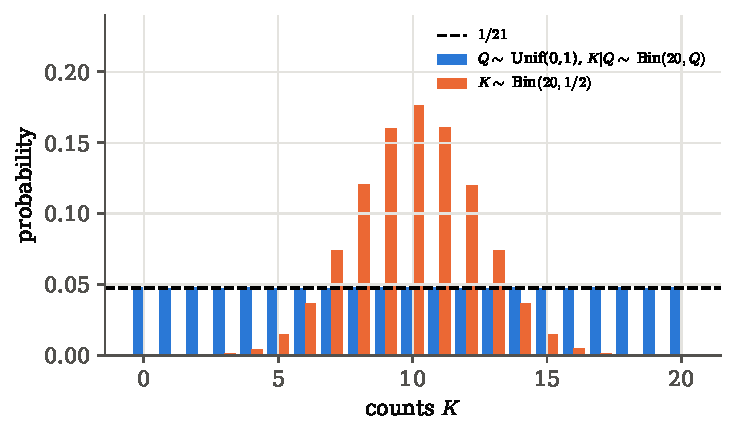
\includegraphics[width=0.72\linewidth]{figures/ch01/hierarchical_counts.pdf}
\caption{Counts out of $20$ photons. Blue: each pixel has its own efficiency,
drawn uniformly; the counts are spread evenly over $0,\dots,20$ at the height
$1/21$ of the dashed line. Orange: every pixel has efficiency $\tfrac12$; the
counts crowd around $10$. Both have mean $10$, but the variances are $36.7$ and
$5$.}
\label{1b:fig:hierarchical}
\end{figure}

The cross term $\E[(X-\mu_X)(Y-\mu_Y)]$ that appeared in the variance of a
sum measures how two variables move together. Together with the averages and
spreads above, it describes the \emph{relation} between two variables at the
level of second moments.
\section{Covariance and correlation: how two variables move together}
\label{1b:sec:covariance}

Two readout channels of a calorimeter sit on the same electronics board. Each
channel records its own signal plus a common pedestal noise that the board
adds to both: $X_1=S_1+N$ and $X_2=S_2+N$, with $S_1$, $S_2$ and $N$
independent. Looked at one at a time, each channel is just a noisy number.
Looked at together, they tend to go up and down together, because whenever
the pedestal $N$ fluctuates high, both readings are pulled up. Nothing about
the individual distributions reveals this. It is a property of the joint
distribution, and the variance of a sum, \eqref{1b:eq:var-sum}, has already
shown us the number that measures it: the cross term
$\E\bigl[(X-\mu_X)(Y-\mu_Y)\bigr]$.

That number is the covariance. Its dimensionless version is the correlation
coefficient. Both detect linear co-movement and miss everything else. For
many variables the second moments collect into a covariance matrix, and a
linear change of variables moves it by the rule $\Cmat'=A\Cmat A\T$. Every
error bar on a derived quantity, every Fisher forecast of \cref{ch:10} and
every $\chi^2$ of correlated band powers in \cref{ch:07,ch:08} is built from
this matrix. Three questions organise the topic.
\begin{enumerate}[leftmargin=1.6em,itemsep=1pt]
  \item How do we measure whether ``$X$ above its mean'' goes with ``$Y$ above
        its mean''?
  \item What does a zero value of that measure tell us, and what does it not?
  \item For a vector of variables, how do the second moments change when we
        form linear combinations, and can we always find combinations that are
        uncorrelated?
\end{enumerate}

\subsection{Covariance and the correlation coefficient}

\begin{workdef}[covariance, correlation coefficient]
For $X,Y$ with means $\mu_X,\mu_Y$ and standard deviations $\sigma_X,\sigma_Y$,
the \newterm{covariance} and the \newterm{correlation coefficient} are
\begin{equation}
  \Cov(X,Y)=\E\bigl[(X-\mu_X)(Y-\mu_Y)\bigr],\qquad
  \rho_{XY}=\frac{\Cov(X,Y)}{\sigma_X\,\sigma_Y} .
  \label{1b:eq:cov}
\end{equation}
$\Cov$ has the units of $X$ times those of $Y$ \unpack{positive if the two
tend to be on the same side of their means}. $\rho$ is a pure number between
$-1$ and $1$.
\emph{Operational test:} the average of $(x_j-\bar x)(y_j-\bar y)$ over many
simulated pairs, \texttt{np.cov} and \texttt{np.corrcoef} in Python.
\end{workdef}

The definition is read off a scatter plot \srcref{Cowan}{pp.~18--19}. Put the
origin at $(\mu_X,\mu_Y)$ (\cref{1b:fig:quadrants}). A point in the upper-right
or lower-left quadrant has deviations of the same sign, so its product
$(x-\mu_X)(y-\mu_Y)$ is positive. A point in the other two quadrants
contributes a negative product. The covariance is the probability-weighted
balance of the two. A cloud tilted up to the right puts more mass in the
positive quadrants and has $\Cov>0$. A cloud tilted down has $\Cov<0$. A cloud
with as much mass in the negative quadrants as in the positive ones has
$\Cov=0$, whatever its shape.

\begin{figure}[htbp]
\centering
\begin{tikzpicture}[scale=0.9]
  \fill[formblue!10] (0,0) rectangle (3,2.2);
  \fill[formblue!10] (0,0) rectangle (-3,-2.2);
  \fill[bdryred!8] (0,0) rectangle (-3,2.2);
  \fill[bdryred!8] (0,0) rectangle (3,-2.2);
  \draw[->] (-3.2,0) -- (3.3,0) node[right,lbl] {$x$};
  \draw[->] (0,-2.4) -- (0,2.5) node[above,lbl] {$y$};
  \draw[thick,formblue,rotate=30] (0,0) ellipse (2.6 and 0.9);
  \draw[formblue,rotate=30] (0,0) ellipse (1.3 and 0.45);
  \node[lbl,formblue!70!black] at (2.2,1.75) {$+$};
  \node[lbl,formblue!70!black] at (-2.2,-1.75) {$+$};
  \node[lbl,bdryred] at (-2.2,1.75) {$-$};
  \node[lbl,bdryred] at (2.2,-1.75) {$-$};
  \fill (0,0) circle (1.2pt);
  \node[lbl,anchor=north west] at (0.35,-0.75) {$(\mu_X,\mu_Y)$};
  \node[lbl,align=left,anchor=west] at (3.5,1.0)
     {$(x-\mu_X)(y-\mu_Y)>0$\\ in the blue quadrants};
  \node[lbl,align=left,anchor=west] at (3.5,-1.0)
     {$(x-\mu_X)(y-\mu_Y)<0$\\ in the red quadrants};
\end{tikzpicture}
\caption{Reading the sign of a covariance. The ellipses are contours of a
density tilted up to the right. Most of its probability sits in the blue
quadrants, where the two deviations have the same sign, so the average of
their product, the covariance, is positive.}
\label{1b:fig:quadrants}
\end{figure}

Expanding the product gives the form used in computation
\mainref{Thm.~3.19, p.~52}:
\begin{align}
  \Cov(X,Y)
  &\eqby{1} \E\bigl[XY-\mu_YX-\mu_XY+\mu_X\mu_Y\bigr]\nonumber\\
  &\eqby{2} \E(XY)-\mu_Y\mu_X-\mu_X\mu_Y+\mu_X\mu_Y
   = \E(XY)-\E(X)\,\E(Y) .
  \label{1b:eq:cov-short}
\end{align}
\begin{explain}
  \item Multiply out $(X-\mu_X)(Y-\mu_Y)$.
  \item Linearity; $\mu_X,\mu_Y$ are constants.
\end{explain}
With $Y=X$ this is the variance shortcut \eqref{1b:eq:var-short}:
$\Cov(X,X)=\Var(X)$. Constants shifted onto either variable drop out, and the
covariance is linear in each argument separately:
\begin{equation}
  \Cov\Bigl(\sum_{i}a_iX_i,\ \sum_{j}b_jY_j\Bigr)=\sum_{i}\sum_{j}a_ib_j\,\Cov(X_i,Y_j)
  \label{1b:eq:bilinear}
\end{equation}
\mainref{Exercise~3.14, p.~60}. To see it, note that the deviation of
$\sum_ia_iX_i$ from its mean is $\sum_ia_i(X_i-\mu_{X_i})$, do the same for
the $Y$'s, multiply the two sums term by term and take the expectation of
each term. Setting both sums equal gives the variance of any linear
combination \mainref{Thm.~3.20, p.~52},
\begin{equation}
  \Var\Bigl(\sum_ia_iX_i\Bigr)=\sum_ia_i^2\Var(X_i)+2\sum_{i<j}a_ia_j\Cov(X_i,X_j),
  \label{1b:eq:var-comb}
\end{equation}
and in particular $\Var(X\pm Y)=\Var(X)+\Var(Y)\pm2\Cov(X,Y)$.

\paragraph{Example: the shared pedestal.}
Return to the two calorimeter channels of the opening, $X_1=S_1+N$ and
$X_2=S_2+N$, which share the pedestal noise $N$. Take $\Var(S_1)=\Var(S_2)=\sigma_S^2$ and
$\Var(N)=\sigma_N^2$. By \eqref{1b:eq:bilinear},
\begin{align*}
  \Cov(X_1,X_2)
  &\eqby{1} \Cov(S_1,S_2)+\Cov(S_1,N)+\Cov(N,S_2)+\Cov(N,N)
   \eqby{2} \sigma_N^2 ,
\end{align*}
\begin{explain}
  \item Bilinearity with $X_1=S_1+N$, $X_2=S_2+N$.
  \item Independent variables have zero covariance (shown below); $\Cov(N,N)=\Var(N)$.
\end{explain}
so $\rho=\sigma_N^2/(\sigma_S^2+\sigma_N^2)$, which is $\tfrac12$ when the
signal and the pedestal fluctuate equally. Now form the difference. By
\eqref{1b:eq:var-comb},
$\Var(X_1-X_2)=2(\sigma_S^2+\sigma_N^2)-2\sigma_N^2=2\sigma_S^2$: the common
noise has cancelled completely. The sum has $\Var(X_1+X_2)=2\sigma_S^2+4\sigma_N^2$:
it is doubled. This is common-mode rejection, and it is why differential
measurements are powerful. A gravitational-wave interferometer reads the
\emph{difference} of its two arm lengths, so the laser noise common to both
arms cancels to first order.

\subsection{Why \texorpdfstring{$\abs\rho\le1$}{|rho| <= 1}, and what \texorpdfstring{$\rho=\pm1$}{rho = +-1} means}

The correlation coefficient removes the units by dividing by both standard
deviations. That it then lies in $[-1,1]$ follows from one observation
\srcref{CasellaBerger}{Thm.~4.5.7}: the mean of a square is never negative.
For every real $t$ let
\begin{align*}
  h(t)
  &\eqby{1} \E\Bigl[\bigl(t(X-\mu_X)+(Y-\mu_Y)\bigr)^2\Bigr]
   \eqby{2} t^2\sigma_X^2+2t\,\Cov(X,Y)+\sigma_Y^2
   \relby{3}{\ge} 0 .
\end{align*}
\begin{explain}
  \item Definition of $h$, the mean square of a combination of the two
        deviations.
  \item Expand the square and use linearity.
  \item The expectation of a non-negative quantity is non-negative.
\end{explain}
A quadratic in $t$ that is never negative has at most one real root, so its
discriminant is not positive: $4\Cov(X,Y)^2-4\sigma_X^2\sigma_Y^2\le0$, that
is, $\abs{\Cov(X,Y)}\le\sigma_X\sigma_Y$, or $-1\le\rho\le1$. Equality,
$\abs\rho=1$, means the discriminant is zero, so $h(t_0)=0$ for one $t_0$,
namely $t_0=-\Cov(X,Y)/\sigma_X^2$. A non-negative variable with zero mean is
zero with probability one, so $Y-\mu_Y=-t_0(X-\mu_X)$: the points lie exactly
on a straight line with slope $a=-t_0=\Cov/\sigma_X^2$, which has the sign of
$\rho$. Conversely if $Y=aX+b$ then $\Cov(X,Y)=a\sigma_X^2$ and
$\sigma_Y=\abs a\sigma_X$, so $\rho=a/\abs a=\pm1$ \mainref{Thm.~3.19, p.~52}.

In the language of vectors this is the Cauchy--Schwarz inequality. Centred
random variables form a vector space with the inner product
$\langle U,V\rangle=\E(UV)$, the length of $U$ is its standard deviation,
and $\rho$ is the cosine of the angle between $X-\mu_X$ and $Y-\mu_Y$. It is
$\pm1$ when the two ``vectors'' are parallel, $0$ when they are orthogonal. A
quantum physicist will recognise the normalised overlap
$\abs{\langle\psi\vert\phi\rangle}/(\norm\psi\norm\phi)\le1$. Because it is a
cosine, $\rho$ is unchanged by shifting or by rescaling either variable with
a positive factor: it does not care whether energies are in GeV or TeV.

\Cref{1b:fig:correlation-gallery} calibrates the eye. With 1500 points from
bivariate Gaussians of unit variances and $\rho=-0.8,\,0,\,0.5,\,0.95$, the
sample correlations are $\OneBGalRa$, $\OneBGalRb$, $\OneBGalRc$ and
$\OneBGalRd$. A correlation of $0.5$ is a visibly tilted but still fat cloud;
it takes $\rho$ close to $1$ to make a thin line.

\begin{figure}[htbp]
\centering
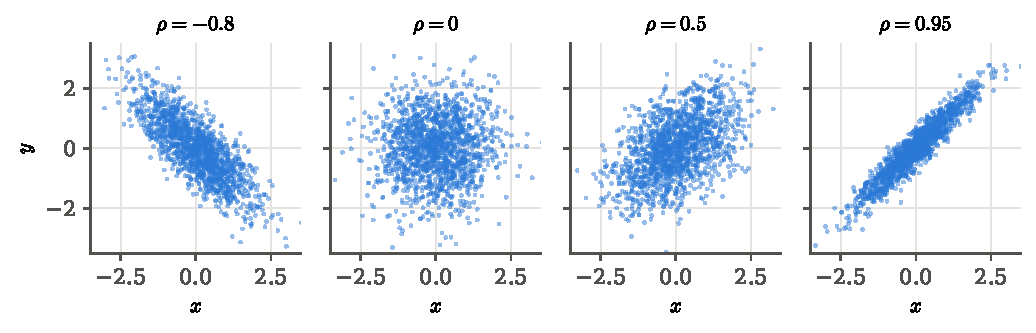
\includegraphics[width=\linewidth]{figures/ch01/correlation_gallery.pdf}
\caption{Clouds of 1500 draws from bivariate Gaussians with unit variances and
four values of the correlation coefficient. The sign of $\rho$ gives the
direction of the tilt; its size says how tightly the points hug a straight
line.}
\label{1b:fig:correlation-gallery}
\end{figure}

\subsection{Zero correlation is not independence}

If $X$ and $Y$ are independent, $\E(XY)=\E(X)\E(Y)$ by
\eqref{1b:eq:product-mean}, and \eqref{1b:eq:cov-short} gives $\Cov(X,Y)=0$.
The converse is false \mainref{Thm.~3.19, p.~52}. The standard
counterexample shows why. Let $X\sim\Normal(0,1)$ and
$Y=X^2$. Then $Y$ is completely determined by $X$, the strongest dependence
there is. Yet
\begin{align*}
  \Cov(X,Y)
  &\eqby{1} \E(X\cdot X^2)-\E(X)\,\E(X^2)
   \eqby{2} \E(X^3)-0\cdot1
   \eqby{3} 0 .
\end{align*}
\begin{explain}
  \item Shortcut \eqref{1b:eq:cov-short} with $Y=X^2$.
  \item $\E(X)=0$ and $\E(X^2)=\Var(X)=1$.
  \item $\E(X^3)=\int x^3\varphi(x)\,\dd x=0$: the integrand is odd because
        the Gaussian density $\varphi$ is even.
\end{explain}
The covariance vanishes because the relation is symmetric: for every point
$(x,x^2)$ on the right branch of the parabola there is an equally likely
point $(-x,x^2)$ on the left, and their products of deviations cancel
\srcref{Cowan}{Fig.~1.10}. The correlation coefficient measures how well a
\emph{straight line} fits, and the best straight line through a symmetric
parabola is flat.

\begin{figure}[htbp]
\centering
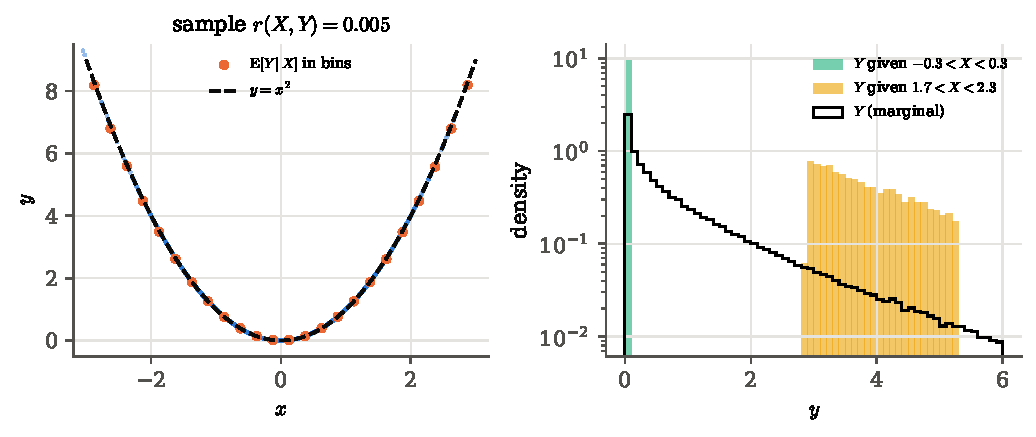
\includegraphics[width=\linewidth]{figures/ch01/zero_correlation.pdf}
\caption{Left: draws of $(X,X^2)$ with $X$ Gaussian. The points lie exactly on
the parabola, the binned conditional mean $\E(Y\given X)$ (orange) follows it,
and yet the sample correlation is essentially zero. Right: the distribution of
$Y$ for $X$ near $0$ and for $X$ near $2$ (logarithmic density axis). The two
conditional distributions do not even overlap, so knowing $X$ changes
everything we know about $Y$, which is the opposite of independence.}
\label{1b:fig:zero-corr}
\end{figure}

\Cref{1b:fig:zero-corr} shows it numerically. With $\OneBZeroN$ draws the
sample correlation of $X$ and $Y$ is $\OneBZeroRxy$. The dependence is all
there: the correlation of $Y$ with $\abs X$ (a monotone function of $X$ on
each branch) is $\OneBZeroRabsxy$, and the conditional distributions of $Y$
in two slices of $X$ are completely different. \srcref{CasellaBerger}{Ex.~4.5.9}
gives a version with noise, $Y=X^2+Z$, with the same conclusion. Operationally:
before concluding that two quantities are unrelated because their correlation
is small, plot them.

There is a ladder of conditions between independence and zero correlation. If
the conditional mean of $X$ does not depend on $Y$, $\E(X\given Y=y)=c$ for all
$y$, then $X$ and $Y$ are uncorrelated \mainref{Exercise~3.18, p.~61}:
\begin{align*}
  \E(XY)
  &\eqby{1} \E\bigl[\E(XY\given Y)\bigr]
   \eqby{2} \E\bigl[Y\,\E(X\given Y)\bigr]
   \eqby{3} c\,\E(Y)
   \eqby{4} \E(X)\,\E(Y) .
\end{align*}
\begin{explain}
  \item Iterated expectations \eqref{1b:eq:iterated}.
  \item Given $Y$, the factor $Y$ is known and comes out.
  \item $\E(X\given Y)=c$.
  \item $\E(X)=\E[\E(X\given Y)]=c$.
\end{explain}
The same two steps show that if $\E(Y\given X)=X$ then $\E(XY)=\E(X^2)$ and
$\E(Y)=\E(X)$, so $\Cov(X,Y)=\Var(X)$ \mainref{Exercise~3.21, p.~61}. So
independence implies a constant conditional mean, which implies zero
correlation, and neither implication reverses (in the parabola example
$\E(Y\given X)=X^2$ is far from constant).

For one family the ladder collapses. If $(X,Y)$ is bivariate Gaussian
\eqref{1b:eq:bvn} with $\rho=0$, the cross term $-2\rho xy/(\sigma_x\sigma_y)$
in the exponent vanishes, the exponent splits into an $x$ part plus a $y$
part, and the density factorises into $f_X(x)f_Y(y)$. For jointly Gaussian
variables, uncorrelated means independent. This is why the sum and the
difference of two equally noisy Gaussian channels in \cref{1b:ex:sum-diff}
came out independent. They are jointly Gaussian, and the sum-and-difference
example of the next subsection shows that they are uncorrelated.

\begin{pitfall}[Gaussian marginals do not make a Gaussian pair]
The shortcut ``uncorrelated $\Rightarrow$ independent'' needs the variables to
be \emph{jointly} Gaussian, not just each Gaussian. Let $X\sim\Normal(0,1)$ and
let $S=\pm1$ be an independent fair sign. Then $Y=SX$ is also $\Normal(0,1)$
(flipping the sign of a symmetric variable changes nothing), and
$\Cov(X,Y)=\E(S)\E(X^2)=0$. But $\abs Y=\abs X$ always, so the two are
strongly dependent. The pair lives on the two diagonals $y=\pm x$, which no
bivariate Gaussian does.
\end{pitfall}

\subsection{The covariance matrix and how linear maps move it}

With many variables we collect them into a column vector
$\bm X=(X_1,\dots,X_k)\T$ with mean vector $\bm\mu=(\E X_1,\dots,\E X_k)\T$. All
the variances and covariances go into one matrix, the
\newterm{covariance matrix} (``variance--covariance matrix'' in
\mainref{p.~53}, ``error matrix'' in \srcref{Cowan}{p.~18}):
\begin{equation}
  \Cmat_{ij}=\Cov(X_i,X_j),\qquad
  \Cmat=\E\bigl[(\bm X-\bm\mu)(\bm X-\bm\mu)\T\bigr]
  =\begin{pmatrix}
     \Var(X_1) & \Cov(X_1,X_2) & \cdots\\
     \Cov(X_2,X_1) & \Var(X_2) & \cdots\\
     \vdots & & \ddots
   \end{pmatrix}.
  \label{1b:eq:covmat}
\end{equation}
The outer product $(\bm X-\bm\mu)(\bm X-\bm\mu)\T$ is a $k\times k$ matrix whose
$(i,j)$ entry is $(X_i-\mu_i)(X_j-\mu_j)$, and the expectation is taken entry
by entry. The matrix is symmetric, its diagonal holds the variances, and it
is positive semi-definite: for any fixed vector $\bm a$,
\begin{align*}
  \bm a\T\Cmat\,\bm a
  &\eqby{1} \sum_{i,j}a_ia_j\Cov(X_i,X_j)
   \eqby{2} \Var\bigl(\bm a\T\bm X\bigr)
   \relby{3}{\ge} 0 .
\end{align*}
\begin{explain}
  \item Write out the quadratic form.
  \item Bilinearity \eqref{1b:eq:bilinear} with $b_j=a_j$ and $Y_j=X_j$.
  \item A variance is never negative.
\end{explain}
So all eigenvalues of $\Cmat$ are $\ge0$. A zero eigenvalue means some
combination $\bm a\T\bm X$ has zero variance, i.e.\ is a constant: the
variables obey an exact linear constraint (as the multinomial counts below do).
Dividing entry $(i,j)$ by $\sigma_i\sigma_j$ gives the correlation matrix, with
ones on the diagonal.

Now let $\bm Y=A\bm X+\bm b$ for a fixed $m\times k$ matrix $A$ and vector $\bm b$.
Linearity gives $\E\bm Y=A\bm\mu+\bm b$, and \mainref{Lemma~3.21, p.~54}
\begin{align}
  \Cmat_{\bm Y}
  &\eqby{1} \E\bigl[(A\bm X-A\bm\mu)(A\bm X-A\bm\mu)\T\bigr]
   \eqby{2} \E\bigl[A(\bm X-\bm\mu)(\bm X-\bm\mu)\T A\T\bigr]
   \eqby{3} A\,\Cmat\,A\T .
  \label{1b:eq:ACAT}
\end{align}
\begin{explain}
  \item Definition \eqref{1b:eq:covmat} for $\bm Y$; the shift $\bm b$ cancels
        in $\bm Y-\E\bm Y$.
  \item $(A\bm v)\T=\bm v\T A\T$.
  \item $A$ is constant and comes out of the entry-by-entry expectation on both
        sides (linearity).
\end{explain}
In components, $(\Cmat_{\bm Y})_{ij}=\sum_{k,l}A_{ik}A_{jl}\Cov(X_k,X_l)$
\srcref{Cowan}{(1.62)}, which is just \eqref{1b:eq:bilinear}. For a single
combination, $A=\bm a\T$ is one row and $\Var(\bm a\T\bm X)=\bm a\T\Cmat\bm a$,
the quadratic form above. The covariance matrix transforms like a rank-2
tensor, $C'_{ij}=A_{ik}A_{jl}C_{kl}$; the inertia tensor and the stress tensor
transform the same way.

\begin{keyidea}[Linear maps move covariance by sandwiching]
If $\bm Y=A\bm X+\bm b$ then $\E\bm Y=A\,\E\bm X+\bm b$ and
$\Cmat_{\bm Y}=A\,\Cmat_{\bm X}A\T$, exactly, for any distribution.
\end{keyidea}

\paragraph{Example: sum and difference of two channels.}
Take $\Cmat=\begin{psmallmatrix}\sigma_1^2 & c\\ c & \sigma_2^2\end{psmallmatrix}$
and $A=\begin{psmallmatrix}1&1\\1&-1\end{psmallmatrix}$, so
$Y_1=X_1+X_2$ and $Y_2=X_1-X_2$. Then
\begin{align*}
  A\,\Cmat\,A\T
  &\eqby{1} \begin{pmatrix}\sigma_1^2+c & c+\sigma_2^2\\ \sigma_1^2-c & c-\sigma_2^2\end{pmatrix}
            \begin{pmatrix}1&1\\1&-1\end{pmatrix}
   \eqby{2} \begin{pmatrix}\sigma_1^2+\sigma_2^2+2c & \sigma_1^2-\sigma_2^2\\
                           \sigma_1^2-\sigma_2^2 & \sigma_1^2+\sigma_2^2-2c\end{pmatrix}.
\end{align*}
\begin{explain}
  \item First product $A\Cmat$, row by column; $A\T=A$ here.
  \item Second product; e.g.\ the $(1,2)$ entry is
        $(\sigma_1^2+c)-(c+\sigma_2^2)$.
\end{explain}
The diagonal reproduces $\Var(X_1\pm X_2)=\sigma_1^2+\sigma_2^2\pm2c$. The new
off-diagonal entry, $\Cov(X_1+X_2,X_1-X_2)=\sigma_1^2-\sigma_2^2$, is zero
whenever the two channels are equally noisy, whatever their correlation $c$.
With $\Cmat=\sigma^2\Id$ we get $A\Cmat A\T=2\sigma^2\Id$, and since the pair is
jointly Gaussian that is the independence of \cref{1b:ex:sum-diff}. For
the numerical case $\sigma_1^2=4$, $\sigma_2^2=1$, $c=1.8$ the prediction is
$\begin{psmallmatrix}8.6&3\\3&1.4\end{psmallmatrix}$, and the sample covariance
of $\OneBCovN$ simulated pairs is
$\begin{psmallmatrix}\OneBCYaa&\OneBCYab\\\OneBCYab&\OneBCYbb\end{psmallmatrix}$.

\paragraph{Example: the multinomial covariance.}
Throw $n$ events into $k$ histogram bins with probabilities $p_1,\dots,p_k$
(\cref{1b:sec:joint}), and let $X_i$ be the count in bin $i$. Each $X_i$ is
binomial, $\Var(X_i)=np_i(1-p_i)$. To get the covariance of two bins, merge
them: $X_i+X_j$ counts the events that fell in either, so it is
$\mathrm{Binomial}(n,p_i+p_j)$ \mainref{p.~54}. Then
\begin{align*}
  2\Cov(X_i,X_j)
  &\eqby{1} \Var(X_i+X_j)-\Var(X_i)-\Var(X_j)\\
  &\eqby{2} n(p_i+p_j)(1-p_i-p_j)-np_i(1-p_i)-np_j(1-p_j)
   \eqby{3} -2np_ip_j ,
\end{align*}
\begin{explain}
  \item \eqref{1b:eq:var-comb} for $X_i+X_j$, solved for the covariance.
  \item Binomial variances of the merged bin and of each bin.
  \item Expand: the linear terms cancel, and
        $-(p_i+p_j)^2+p_i^2+p_j^2=-2p_ip_j$.
\end{explain}
so $\Cov(X_i,X_j)=-np_ip_j$ for $i\neq j$. Histogram bins with a fixed total
are anticorrelated: an extra event in one bin is an event missing from the
others. The covariance matrix has a zero eigenvalue along $\bm a=(1,\dots,1)$,
because $\sum_iX_i=n$ is exactly constant. (If the total itself is a Poisson
count, as for a collider run of fixed luminosity, the bins become
independent Poisson variables; see \cref{ch:02}.)

\subsection{Diagonalising: the principal axes of the error ellipse}

Correlated variables are awkward: we cannot read off the uncertainty of one
without the other. Can a linear change of variables always make them
uncorrelated? Yes, and it is a rotation \srcref{Cowan}{\S1.7}. Because $\Cmat$
is real and symmetric, it has $k$ orthonormal eigenvectors $\bm r_1,\dots,\bm r_k$,
$\Cmat\bm r_j=\lambda_j\bm r_j$, with $\lambda_j\ge0$ by positive
semi-definiteness. Put them as the columns of an orthogonal matrix $R$ and
take $\bm W=R\T\bm X$, so $W_i=\bm r_i\T\bm X$ is the component of $\bm X$ along
$\bm r_i$. By \eqref{1b:eq:ACAT} with $A=R\T$,
\begin{align*}
  (\Cmat_{\bm W})_{ij}
  &\eqby{1} \bigl(R\T\Cmat R\bigr)_{ij}
   \eqby{2} \bm r_i\T\Cmat\,\bm r_j
   \eqby{3} \lambda_j\,\bm r_i\T\bm r_j
   \eqby{4} \lambda_j\,\delta_{ij} .
\end{align*}
\begin{explain}
  \item The sandwich rule with $A=R\T$.
  \item Row $i$ of $R\T$ is $\bm r_i\T$ and column $j$ of $R$ is $\bm r_j$.
  \item Eigenvalue equation.
  \item Orthonormality of the eigenvectors.
\end{explain}
The new variables are uncorrelated and their variances are the eigenvalues
\srcref{Cowan}{(1.65)}. Geometrically, the contours of a Gaussian density with
covariance $\Cmat$ are ellipses (ellipsoids) whose axes point along the
eigenvectors, with semi-axes $\sqrt{\lambda_j}$ at ``$1\sigma$''. The rotation
simply turns the coordinate axes onto the principal axes of this
\newterm{error ellipse}, exactly like rotating onto the principal axes of an
inertia tensor or onto the normal modes of coupled oscillators.

In two dimensions everything is explicit. Write
$\Cmat=\begin{psmallmatrix}\sigma_1^2&c\\c&\sigma_2^2\end{psmallmatrix}$ with
$c=\rho\sigma_1\sigma_2$. The eigenvalues solve
$\det(\Cmat-\lambda\Id)=\lambda^2-(\sigma_1^2+\sigma_2^2)\lambda+\sigma_1^2\sigma_2^2-c^2=0$,
so
\begin{equation}
  \lambda_\pm=\tfrac12\Bigl[\sigma_1^2+\sigma_2^2
     \pm\sqrt{(\sigma_1^2+\sigma_2^2)^2-4(1-\rho^2)\sigma_1^2\sigma_2^2}\Bigr]
  \label{1b:eq:eig2}
\end{equation}
\srcref{Cowan}{(1.69)}. For the rotation angle, rotate by $\theta$,
$W_1=\cos\theta\,X_1+\sin\theta\,X_2$ and $W_2=-\sin\theta\,X_1+\cos\theta\,X_2$,
and demand zero covariance:
\begin{align*}
  \Cov(W_1,W_2)
  &\eqby{1} -\sin\theta\cos\theta\,\sigma_1^2+(\cos^2\theta-\sin^2\theta)\,c
            +\sin\theta\cos\theta\,\sigma_2^2\\
  &\eqby{2} \tfrac12\sin2\theta\,(\sigma_2^2-\sigma_1^2)+c\cos2\theta ,
\end{align*}
\begin{explain}
  \item Bilinearity \eqref{1b:eq:bilinear}.
  \item Double-angle formulas.
\end{explain}
which vanishes for $\tan2\theta=2c/(\sigma_1^2-\sigma_2^2)$
\srcref{Cowan}{(1.71)}. For $\sigma_1^2=4$, $\sigma_2^2=1$, $c=1.8$ (so
$\rho=0.9$): $\tan2\theta=1.2$, $\theta=25.1^\circ$, and
\eqref{1b:eq:eig2} gives $\lambda=(5\pm\sqrt{21.96})/2=\OneBLamB$ and
$\OneBLamA$. The simulated rotated variables have variances $\OneBCWbb$ and
$\OneBCWaa$ and covariance $\OneBCWab$ (\cref{1b:fig:cov-transform}, right).
The long axis carries almost all the variance: nearly all the scatter of the
two channels is in one combination.

The same algebra run backwards generates correlated variables. If $\bm Z$ has
independent standard normal components, $\Cmat_{\bm Z}=\Id$, and
$\bm X=L\bm Z$ has covariance $L\Id L\T=LL\T$. So any factorisation
$\Cmat=LL\T$ gives a recipe. The standard one is the Cholesky factor, a lower
triangular $L$; for $2\times2$,
$L=\begin{psmallmatrix}\sigma_1&0\\\rho\sigma_2&\sigma_2\sqrt{1-\rho^2}\end{psmallmatrix}$,
which one checks by multiplying out. Here $L=\begin{psmallmatrix}\OneBLaa&0\\
\OneBLba&\OneBLbb\end{psmallmatrix}$, and the script uses exactly this:

\pyfile[firstline=21,lastline=35,firstnumber=21]{code/ch01/18_covariance_transform.py}{Correlated Gaussians, the sandwich rule and the eigenbasis}

Lines 22--25 build $L$ and generate $\bm X=L\bm Z$ for $\OneBCovN$ pairs; their
sample covariance (line 26) is
$\begin{psmallmatrix}\OneBChataa&\OneBChatab\\\OneBChatab&\OneBChatbb\end{psmallmatrix}$,
the target $\Cmat$. Lines 28--31 apply the sum-and-difference matrix and
compare $A\Cmat A\T$ with the sample covariance of $\bm Y$. Lines 33--35
diagonalise: \texttt{np.linalg.eigh} returns the eigenvalues in ascending order
and the unit eigenvectors as the columns of \texttt{R}, and $\bm W=R\T\bm X$
is uncorrelated.

\begin{figure}[htbp]
\centering
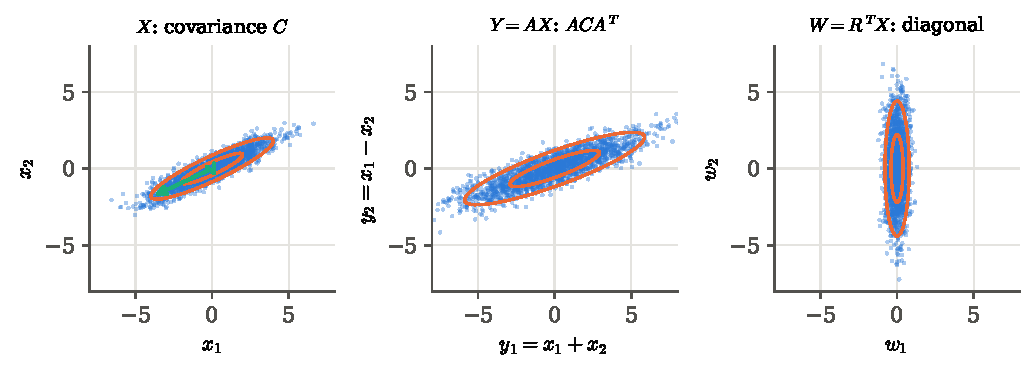
\includegraphics[width=\linewidth]{figures/ch01/covariance_transform.pdf}
\caption{One cloud of correlated pairs seen in three coordinate systems, with
the predicted $1\sigma$ and $2\sigma$ ellipses. Left: the original channels,
with the two eigenvectors of $\Cmat$ drawn as green arrows. Middle: sum and
difference; the ellipse is the one predicted by $A\Cmat A\T$. Right: components
along the eigenvectors; the ellipse is aligned with the axes, so the new
variables are uncorrelated.}
\label{1b:fig:cov-transform}
\end{figure}

\subsection{A first look at error propagation}

Most derived quantities are not linear in the measured ones: a mass from two
momenta, a ratio of two rates, a distance from a flux. If the input
uncertainties are small, we can linearise \srcref{Cowan}{\S1.6}. Expand
$y(\bm x)$ to first order about the means,
$y(\bm x)\approx y(\bm\mu)+\sum_iA_i(x_i-\mu_i)$ with
$A_i=\partial y/\partial x_i$ at $\bm\mu$. The constant does not affect the
spread, and the rest is linear, so the sandwich rule applies to the Jacobian
matrix $A_{ki}=\partial y_k/\partial x_i$:
\begin{equation}
  \E\,y_k\approx y_k(\bm\mu),\qquad
  \Cov(y_k,y_l)\approx\sum_{i,j}\frac{\partial y_k}{\partial x_i}
     \frac{\partial y_l}{\partial x_j}\,\Cmat_{ij},\qquad
  \Cmat_{\bm y}\approx A\,\Cmat\,A\T
  \label{1b:eq:error-prop}
\end{equation}
\srcref{Cowan}{(1.53)--(1.55)}. For a linear map this is exact
\eqref{1b:eq:ACAT}; otherwise it is the first term of an expansion.

\paragraph{Example: products add relative errors in quadrature.}
For $y=x_1x_2$ the Jacobian is $A=(\mu_2,\ \mu_1)$, so
\begin{align*}
  \sigma_y^2
  &\eqby{1} \mu_2^2\sigma_1^2+\mu_1^2\sigma_2^2+2\mu_1\mu_2\,\Cmat_{12},
  &
  \frac{\sigma_y^2}{y^2}
  &\eqby{2} \frac{\sigma_1^2}{\mu_1^2}+\frac{\sigma_2^2}{\mu_2^2}
            +2\frac{\Cmat_{12}}{\mu_1\mu_2} .
\end{align*}
\begin{explain}
  \item \eqref{1b:eq:error-prop} with $\partial y/\partial x_1=x_2$,
        $\partial y/\partial x_2=x_1$ at the means.
  \item Divide by $y^2\approx\mu_1^2\mu_2^2$.
\end{explain}
For uncorrelated inputs, absolute errors add in quadrature for a sum and
relative errors add in quadrature for a product \srcref{Cowan}{(1.59)--(1.60)}.
The approximation fails when $y$ curves appreciably over a range of one
standard deviation; the classic case is $1/x$ with $\sigma_x$ not small
compared with $\mu_x$. Then one simulates (\cref{ch:06}). Error propagation,
and its limits, is developed properly in \cref{ch:03}.

\paragraph{How research uses it.} In a real analysis the covariance matrix is rarely computed on paper. The
band powers of a CMB or galaxy power spectrum measured on a masked, noisy sky
(\cref{ch:07,ch:08}) are correlated in ways no formula captures, so one
simulates $N_s$ mock data sets and uses the sample covariance, the matrix
version of $S_n^2$ with its $1/(N_s-1)$. The $\chi^2$ likelihood needs the
\emph{inverse}, and the inverse of a noisy estimate is biased; it must be
rescaled by $(N_s-p-2)/(N_s-1)$ for $p$ data points \cite{Hartlap2007}. The
Fisher matrix of \cref{ch:10} is the inverse of a forecast parameter
covariance, and its eigenvectors are the principal axes above: the
best- and worst-constrained combinations of parameters. The simulations here
\emph{verified} $A\Cmat A\T$, a known result; in those analyses the same
simulate-and-average machinery is the only way to obtain $\Cmat$ at all.
\section{Moments, generating functions and characteristic functions}
\label{1b:sec:moments}

A physicist has two standard ways of packing a whole function into
something easier to handle. One is a list of moments: the total charge, the
dipole moment and the quadrupole moment of a charge distribution describe it
from far away, better and better as more terms are kept. The other is a
transform: a Fourier or Laplace transform turns a messy operation on
functions into a simple one on their transforms. Probability uses both, and
statistical mechanics has used them all along. The partition function
$Z(\beta)=\int g(E)\,e^{-\beta E}\,\dd E$ is the Laplace transform of the
density of states $g(E)$, and the mean energy and its fluctuations,
$\langle E\rangle=-\partial_\beta\ln Z$ and
$\langle E^2\rangle-\langle E\rangle^2=\partial_\beta^2\ln Z=k_BT^2C_V$, are
read off from its derivatives.

Higher moments describe the shape of a distribution. Two transforms, the
moment generating function and the characteristic function, produce all the
moments at once. Their more important use is a different one: sums. In
\cref{1b:sec:transform} the density of a sum of independent variables was a
convolution \eqref{1b:eq:convolution}, an integral that gets worse with every
term added. After a Fourier transform, convolution becomes multiplication.
That single fact is what makes the central limit theorem of \cref{ch:02}
provable in a few lines. Three questions organise the topic.
\begin{enumerate}[leftmargin=1.6em,itemsep=1pt]
  \item Which numbers beyond the mean and the variance describe the shape of a
        distribution, and do they determine it?
  \item How do we get the distribution of a sum of independent variables
        without doing convolution integrals?
  \item What do we do when the moments, or the transform itself, do not exist?
\end{enumerate}

\subsection{Moments and the shape of a distribution}

The $k$-th \newterm{moment} of $X$ is $\E(X^k)$ and the $k$-th
\newterm{central moment} is $\E\bigl[(X-\mu)^k\bigr]$, assuming
$\E\abs X^k<\infty$ \mainref{p.~49--50} (\srcref{Cowan}{(1.41)--(1.42)} writes
them $\mu_n'$ and $\mu_n$). The first moment is the mean and the second
central moment the variance. The standardised third and fourth central
moments describe shape:
\begin{equation}
  \gamma_1=\frac{\E(X-\mu)^3}{\sigma^3}\ \ \text{(skewness)},\qquad
  \gamma_2=\frac{\E(X-\mu)^4}{\sigma^4}-3\ \ \text{(excess kurtosis)} .
  \label{1b:eq:skew-kurt}
\end{equation}
Both are pure numbers. The skewness is positive when a long tail extends to
the right (the exponential has $\gamma_1=2$), zero for a symmetric
distribution. The $-3$ is chosen so that a Gaussian has $\gamma_2=0$;
distributions with heavier tails than the Gaussian have $\gamma_2>0$. In the
multipole language the mean is the centre of charge, and the variance is the
moment of inertia about it.

A higher moment existing guarantees the lower ones \mainref{Thm.~3.10,
p.~49}. For $j<k$,
\begin{align*}
  \E\abs X^j
  &\eqby{1} \int_{\abs x\le1}\abs x^jf(x)\,\dd x+\int_{\abs x>1}\abs x^jf(x)\,\dd x\\
  &\relby{2}{\le} \int_{\abs x\le1}f(x)\,\dd x+\int_{\abs x>1}\abs x^kf(x)\,\dd x
   \relby{3}{\le} 1+\E\abs X^k .
\end{align*}
\begin{explain}
  \item Split the range at $\abs x=1$.
  \item On $\abs x\le1$, $\abs x^j\le1$. On $\abs x>1$, $\abs x^j\le\abs x^k$
        because $j<k$.
  \item The first integral is at most the total probability $1$; the second is
        at most the full integral of $\abs x^kf$.
\end{explain}
The converse fails, and tails decide: the Cauchy density has no moments at all
(\cref{1b:sec:expectation}), and a density falling like $1/\abs x^{4}$ has a
mean and a variance but no third moment.

Do the moments, if they all exist, determine the distribution? Not always.
Here are two different densities on $x>0$
\srcref{CasellaBerger}{Ex.~2.3.10}:
\[
  f_1(x)=\frac{1}{\sqrt{2\pi}\,x}\,e^{-(\ln x)^2/2},\qquad
  f_2(x)=f_1(x)\bigl[1+\sin(2\pi\ln x)\bigr],
\]
with identical moments of every order. ($f_1$ is the lognormal: $\ln X$ is
standard normal.) With $u=\ln x$, so that $f_1(x)\,\dd x=\varphi(u)\,\dd u$
with $\varphi$ the standard normal density, the extra piece of the $r$-th
moment of $f_2$ is
\begin{align*}
  \int_0^\infty x^rf_1(x)\sin(2\pi\ln x)\,\dd x
  &\eqby{1} \int_{-\infty}^{\infty}e^{ru}\varphi(u)\sin(2\pi u)\,\dd u
   \eqby{2} e^{r^2/2}\int_{-\infty}^{\infty}\varphi(u-r)\sin(2\pi u)\,\dd u\\
  &\eqby{3} e^{r^2/2}\int_{-\infty}^{\infty}\varphi(y)\sin(2\pi y)\,\dd y
   \eqby{4} 0 .
\end{align*}
\begin{explain}
  \item Substitute $x=e^u$; $x^r=e^{ru}$.
  \item Complete the square: $ru-u^2/2=r^2/2-(u-r)^2/2$.
  \item Substitute $y=u-r$. For integer $r$, $\sin(2\pi(y+r))=\sin(2\pi y)$.
  \item $\varphi$ is even and $\sin$ is odd, so the integrand is odd.
\end{explain}
So $f_1$ and $f_2$ share all moments, $\E X^r=e^{r^2/2}$ for both, though they
are visibly different densities. The problem is again the tails: the moments
grow so fast that they fail to pin down the function. When the support is
bounded, or when the moment generating function below exists in an interval
around $t=0$, the moments do determine the distribution
\srcref{CasellaBerger}{Thm.~2.3.11}.

\subsection{The moment generating function}

The \newterm{moment generating function} (mgf) of $X$ is
\mainref{Def.~3.29, p.~56}
\begin{equation}
  \psi_X(t)=\E\bigl(e^{tX}\bigr)=\int e^{tx}f(x)\,\dd x ,
  \label{1b:eq:mgf}
\end{equation}
for the real $t$ where the expectation is finite. It is the Laplace transform
of the density (with $t\to-t$), and we assume it is finite on some interval
around $t=0$. The name comes from expanding the exponential:
$e^{tX}=\sum_k t^kX^k/k!$, so
\begin{equation}
  \psi_X(t)=\sum_{k=0}^{\infty}\frac{t^k}{k!}\,\E(X^k),
  \qquad\text{hence}\qquad
  \psi_X^{(k)}(0)=\E(X^k) .
  \label{1b:eq:mgf-moments}
\end{equation}
The moments are the Taylor coefficients of $\psi$ at $0$ (times $k!$). Moving
$\E$ through the sum, or through $\dd/\dd t$ as \mainref{p.~56} does, is
legitimate precisely because $\psi$ is finite near $0$.

\paragraph{Example: the exponential.}
For $X\sim\mathrm{Exp}(1)$, $f(x)=e^{-x}$ on $x>0$ \mainref{Ex.~3.30, p.~57}:
\begin{align*}
  \psi_X(t)
  &\eqby{1} \int_0^\infty e^{tx}e^{-x}\,\dd x
   \eqby{2} \int_0^\infty e^{-(1-t)x}\,\dd x
   \eqby{3} \frac{1}{1-t}
   \eqby{4} \sum_{k=0}^\infty t^k\qquad(t<1).
\end{align*}
\begin{explain}
  \item Definition \eqref{1b:eq:mgf}.
  \item Combine the exponents.
  \item The integral converges only for $t<1$; for $t\ge1$ it diverges.
  \item Geometric series, valid for $\abs t<1$.
\end{explain}
Matching with \eqref{1b:eq:mgf-moments}, $\E(X^k)/k!=1$, so $\E(X^k)=k!$: mean
$1$, $\E X^2=2$, variance $2-1=1$, all without an integral beyond the first.
We can run the same computation on data. Replace $\psi$ by the empirical mgf,
the average of $e^{tX_j}$ over simulated draws, and differentiate it
numerically at $0$:

\pyfile[firstline=23,lastline=27,firstnumber=23]{code/ch01/19_characteristic_function.py}{Moments from the empirical mgf}

Line 25 defines $\hat\psi(t)$ as a sample mean over $10^6$ draws; lines 26--27
are the central finite differences for $\psi'(0)$ and $\psi''(0)$ with step
$h=0.01$. They give $\OneBMgfMone$ and $\OneBMgfMtwo$ (exact $1$ and $2$).

\paragraph{Linear changes and sums.}
Two properties make the mgf useful \mainref{Lemma~3.31, p.~57}. For
$Y=aX+b$, $\psi_Y(t)=\E\bigl(e^{t(aX+b)}\bigr)=e^{bt}\psi_X(at)$. For a sum of
independent variables,
\begin{align}
  \psi_{X_1+\dots+X_n}(t)
  &\eqby{1} \E\bigl(e^{tX_1}e^{tX_2}\cdots e^{tX_n}\bigr)
   \eqby{2} \E\bigl(e^{tX_1}\bigr)\cdots\E\bigl(e^{tX_n}\bigr)
   = \prod_{i=1}^n\psi_{X_i}(t) .
  \label{1b:eq:mgf-sum}
\end{align}
\begin{explain}
  \item The exponential of a sum is the product of exponentials.
  \item Independence: the mean of a product of functions of independent
        variables is the product of the means (\cref{1b:sec:expectation}).
\end{explain}
Combined with uniqueness (if two mgfs agree on an interval around $0$, the
distributions are equal, \mainref{Thm.~3.33, p.~57}), this identifies the
distribution of a sum by recognising its mgf.

\paragraph{Example: binomial and Poisson sums.}
A Bernoulli trial has $\psi(t)=(1-p)+pe^t$. A binomial count is a sum of $n$
independent trials, so $\psi(t)=(pe^t+q)^n$ with $q=1-p$
\mainref{Ex.~3.32, p.~57}. Adding two independent binomials with the same $p$
gives $(pe^t+q)^{n_1}(pe^t+q)^{n_2}=(pe^t+q)^{n_1+n_2}$, the mgf of
$\mathrm{Binomial}(n_1+n_2,p)$: pooling two runs of trials is one longer run
\mainref{Ex.~3.34, p.~57}. For a Poisson count,
\begin{align*}
  \psi(t)
  &\eqby{1} \sum_{k=0}^\infty e^{tk}\,\frac{e^{-\lambda}\lambda^k}{k!}
   \eqby{2} e^{-\lambda}\sum_{k=0}^\infty\frac{(\lambda e^t)^k}{k!}
   \eqby{3} e^{-\lambda}e^{\lambda e^t}
   = e^{\lambda(e^t-1)} .
\end{align*}
\begin{explain}
  \item Lazy statistician with the Poisson pmf.
  \item Collect $e^{tk}\lambda^k=(\lambda e^t)^k$.
  \item Exponential series $\sum_ka^k/k!=e^a$.
\end{explain}
Then independent $Y_1\sim\mathrm{Poisson}(\lambda_1)$ and
$Y_2\sim\mathrm{Poisson}(\lambda_2)$ have
$\psi_{Y_1+Y_2}=e^{\lambda_1(e^t-1)}e^{\lambda_2(e^t-1)}=e^{(\lambda_1+\lambda_2)(e^t-1)}$,
so $Y_1+Y_2\sim\mathrm{Poisson}(\lambda_1+\lambda_2)$
\mainref{Ex.~3.35, p.~58}.\footnote{The text writes the sum as
``$Y=Y_1+Y+2$''; it should read $Y=Y_1+Y_2$.} Signal events and background
events counted in the same window form one Poisson count with the summed rate,
the starting point of every counting experiment in \cref{ch:04}.

\paragraph{Example: the Gaussian, by completing the square.}
For $X\sim\Normal(\mu,\sigma^2)$ write $x=\mu+\sigma z$:
\begin{align*}
  \psi_X(t)
  &\eqby{1} e^{\mu t}\int\frac{e^{-z^2/2}}{\sqrt{2\pi}}\,e^{\sigma tz}\,\dd z
   \eqby{2} e^{\mu t}\,e^{\sigma^2t^2/2}\int\frac{e^{-(z-\sigma t)^2/2}}{\sqrt{2\pi}}\,\dd z
   \eqby{3} e^{\mu t+\sigma^2t^2/2} .
\end{align*}
\begin{explain}
  \item $e^{tx}=e^{\mu t}e^{\sigma tz}$, and $f(x)\,\dd x=\varphi(z)\,\dd z$.
  \item Complete the square: $-z^2/2+\sigma tz=-(z-\sigma t)^2/2+\sigma^2t^2/2$.
  \item The remaining integral is a shifted standard normal density, which
        integrates to $1$.
\end{explain}
A sum of independent Gaussians therefore has mgf
$\exp\bigl[(\sum_i\mu_i)t+(\sum_i\sigma_i^2)t^2/2\bigr]$: it is Gaussian, with the
means added and the variances added. The table of \mainref{p.~58} also lists
$\mathrm{Gamma}(\alpha,\beta)$, $\psi(t)=(1-\beta t)^{-\alpha}$ for $t<1/\beta$.
Since an exponential with mean $\beta$ is $\mathrm{Gamma}(1,\beta)$, the sum
of $n$ independent exponential lifetimes has mgf $(1-\beta t)^{-n}$ and is
$\mathrm{Gamma}(n,\beta)$ \mainref{Exercise~3.24, p.~61}. The named distributions
and their mgfs are the subject of \cref{ch:02}.

\paragraph{Cumulants.}
Because sums multiply mgfs, their logarithms add. The
\newterm{cumulant generating function} $K(t)=\ln\psi(t)$ has Taylor
coefficients $K(t)=\sum_n\kappa_nt^n/n!$ called \newterm{cumulants}
\srcref{CasellaBerger}{\S2.6.2}. The first two are
\begin{align*}
  \kappa_1&=K'(0)\eqby{1}\frac{\psi'(0)}{\psi(0)}=\mu,&
  \kappa_2&=K''(0)\eqby{2}\frac{\psi''(0)}{\psi(0)}-\Bigl(\frac{\psi'(0)}{\psi(0)}\Bigr)^2=\sigma^2,
\end{align*}
\begin{explain}
  \item Derivative of a logarithm; $\psi(0)=\E(1)=1$ and $\psi'(0)=\mu$.
  \item Quotient rule, then $\psi''(0)=\E X^2$ and the shortcut
        \eqref{1b:eq:var-short}.
\end{explain}
and $\kappa_3=\E(X-\mu)^3$. For independent $X,Y$ every cumulant adds,
$\kappa_n(X+Y)=\kappa_n(X)+\kappa_n(Y)$. For the Gaussian
$K(t)=\mu t+\sigma^2t^2/2$ exactly, so every cumulant beyond the second is
zero. Non-zero higher cumulants therefore measure non-Gaussianity: the skewness
is $\kappa_3/\kappa_2^{3/2}$. The primordial non-Gaussianity parameter
$f_{\rm NL}$ of cosmology is a third cumulant of this kind, and the
topological summaries of \cref{ch:12} are one way to detect such departures
from Gaussianity.

Return to the partition function $Z(\beta)=\int g(E)\,e^{-\beta E}\,\dd E$ of
the opening. The mgf of the energy in the canonical ensemble is
$\E e^{tE}=Z(\beta-t)/Z(\beta)$, so $K(t)=\ln Z(\beta-t)-\ln Z(\beta)$ and
$\kappa_1=-\partial_\beta\ln Z$, $\kappa_2=\partial^2_\beta\ln Z$: the free
energy is a cumulant generating function.

\subsection{The characteristic function}

The mgf has a weakness: it may not exist. For the Cauchy density
$e^{tx}/(1+x^2)$ grows without bound in one tail for every $t\neq0$, so
$\psi(t)=\infty$. The lognormal $f_1$ above has all its moments, yet
$\psi(t)=\infty$ for every $t>0$, which is how it escapes the uniqueness
theorem. The cure is to put an $i$ in the exponent.

\begin{workdef}[characteristic function]
The \newterm{characteristic function} of $X$ is
\begin{equation}
  \phi_X(t)=\E\bigl(e^{itX}\bigr)=\int e^{itx}f(x)\,\dd x ,\qquad t\in\R ,
  \label{1b:eq:cf}
\end{equation}
\unpack{the Fourier transform of the density}. It always exists, since
$\abs{e^{itx}}=1$ gives $\abs{\phi(t)}\le\int f=1$, and it determines the
distribution uniquely. The density is recovered by the inverse transform
\begin{equation}
  f(x)=\frac{1}{2\pi}\int\phi_X(t)\,e^{-itx}\,\dd t
  \label{1b:eq:cf-inverse}
\end{equation}
whenever $\phi_X$ is integrable.
\emph{Operational test:} the average of $\cos(tX_j)+i\sin(tX_j)$ over draws.
\end{workdef}

(\mainref{p.~56, footnote~2} mentions it in one line;
\srcref{CasellaBerger}{\S2.6.2} states the existence and uniqueness.) In the
Fourier convention used throughout, $\tilde h(f)=\int h(x)e^{-2\pi ifx}\dd x$, the
characteristic function is $\phi(t)=\tilde f(-t/2\pi)$: the same transform with
the sign of the exponent flipped and the frequency measured in radians. The
properties follow directly from \eqref{1b:eq:cf}: $\phi(0)=1$;
$\phi(-t)=\overline{\phi(t)}$; $\phi$ is real if and only if the distribution
is symmetric about $0$; $\phi_{aX+b}(t)=e^{ibt}\phi_X(at)$; the product rule
\eqref{1b:eq:mgf-sum} holds with $it$ in place of $t$; and when the moments
exist, $\phi^{(k)}(0)=i^k\E(X^k)$, so the Taylor expansion near $0$ is
\begin{equation}
  \phi_X(t)=1+i\mu t-\tfrac12\E(X^2)\,t^2+o(t^2) .
  \label{1b:eq:cf-taylor}
\end{equation}
For the Gaussian, replacing $t$ by $it$ in the mgf gives
$\phi(t)=e^{i\mu t-\sigma^2t^2/2}$: the Fourier transform of a Gaussian is a
Gaussian, with the width inverted, as in the uncertainty relation between
position and momentum wave packets.

\paragraph{Example: the uniform and its sums.}
For $U\sim\mathrm{Uniform}(-1,1)$,
\begin{align*}
  \phi_U(t)
  &\eqby{1} \frac12\int_{-1}^{1}e^{itx}\,\dd x
   \eqby{2} \frac12\cdot\frac{e^{it}-e^{-it}}{it}
   \eqby{3} \frac{\sin t}{t} .
\end{align*}
\begin{explain}
  \item Definition \eqref{1b:eq:cf} with density $\tfrac12$ on $(-1,1)$.
  \item Antiderivative $e^{itx}/(it)$.
  \item $e^{it}-e^{-it}=2i\sin t$.
\end{explain}
It is real because $U$ is symmetric, and it is the diffraction pattern of a
single slit, since a uniform density is a slit aperture. The sum of $n$
independent copies has $\phi(t)=(\sin t/t)^n$. For $n=2$, the inverse
transform \eqref{1b:eq:cf-inverse} of $(\sin t/t)^2$ must be the triangle
density $(1-\abs s/2)/2$ on $(-2,2)$ found by convolution in
\cref{1b:ex:triangle}. \Cref{1b:fig:cf} checks both directions numerically.
With $\OneBCfN$ draws, the empirical characteristic functions of $U$, $U_1+U_2$
and $U_1+U_2+U_3$ agree with $(\sin t/t)^n$ to within $\OneBCfMaxDev$ at every
$t$ (the expected sampling noise is about $1/\sqrt{10^5}\approx0.003$ per
point). A numerical inverse Fourier transform of $(\sin t/t)^2$ reproduces the
triangle to within $\OneBCfInvDev$.

\begin{figure}[htbp]
\centering
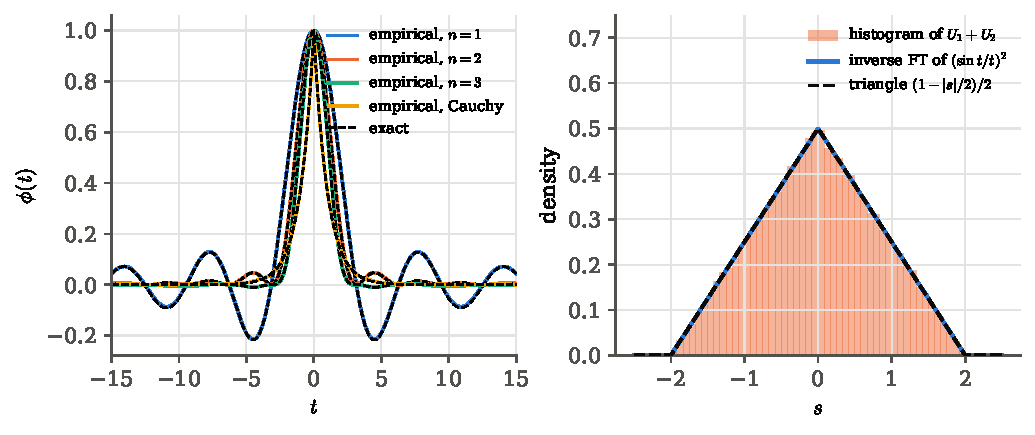
\includegraphics[width=\linewidth]{figures/ch01/characteristic_function.pdf}
\caption{Left: characteristic functions estimated from simulated draws
(coloured) against the exact ones (black dashed): $(\sin t/t)^n$ for sums of
$n=1,2,3$ uniforms, which narrow and flatten their side lobes as $n$ grows,
and $e^{-\abs t}$ for the Cauchy, with its kink at $t=0$. Right: the
histogram of $U_1+U_2$, the numerical inverse transform of $(\sin t/t)^2$, and
the exact triangle lie on top of each other.}
\label{1b:fig:cf}
\end{figure}

The picture behind this is the convolution theorem, drawn in
\cref{1b:fig:conv-theorem}. For independent $X$ and $Y$ the density of $X+Y$ is
the convolution $f_X*f_Y$ \eqref{1b:eq:convolution}, and its characteristic
function is the product $\phi_X\phi_Y$. Going around the square the long
way, through Fourier space, replaces an integral by a multiplication.

\begin{figure}[htbp]
\centering
\begin{tikzpicture}[
  nd/.style={draw=accent,rounded corners=2pt,fill=ideabg,align=center,
             font=\small,minimum width=3.4cm,minimum height=0.9cm},
  ar/.style={->,thick,accent}]
  \node[nd] (f)   at (0,1.8)  {densities $f_X,\ f_Y$};
  \node[nd] (fs)  at (6.4,1.8) {density of $X+Y$:\\ $f_X*f_Y$};
  \node[nd] (p)   at (0,0)    {cfs $\phi_X,\ \phi_Y$};
  \node[nd] (ps)  at (6.4,0)  {cf of $X+Y$:\\ $\phi_X\,\phi_Y$};
  \draw[ar] (f) -- (fs);
  \draw[ar] (f) -- (p);
  \draw[ar] (p) -- (ps);
  \draw[ar] (ps) -- (fs);
  \node[lbl,anchor=south] at (3.2,1.9) {convolve (hard)};
  \node[lbl,anchor=north] at (3.2,-0.1) {multiply (easy)};
  \node[lbl,anchor=east] at (-0.1,0.9) {Fourier transform};
  \node[lbl,anchor=west] at (6.5,0.9) {inverse transform};
\end{tikzpicture}
\caption{Two routes from the densities of two independent variables to the
density of their sum. The top route is the convolution integral. The bottom
route transforms each density, multiplies the transforms, and transforms back.}
\label{1b:fig:conv-theorem}
\end{figure}

\begin{keyidea}[Sums of independent variables]
For independent $X_1,\dots,X_n$ the characteristic function of the sum is
the product $\prod_i\phi_{X_i}(t)$, and the characteristic function determines
the distribution. The same holds for the mgf wherever it exists.
\end{keyidea}

\paragraph{Example: the Cauchy, and why its average never settles.}
The characteristic function of the Cauchy density is $e^{-\abs t}$. The
cleanest proof applies the inversion formula \eqref{1b:eq:cf-inverse} to
$e^{-\abs t}$ and checks that the result is the Cauchy density:
\begin{align*}
  \frac1{2\pi}\int_{-\infty}^{\infty}e^{-\abs t}e^{-itx}\,\dd t
  &\eqby{1} \frac1{2\pi}\Bigl[\int_0^\infty e^{-t(1+ix)}\,\dd t+\int_0^\infty e^{-t(1-ix)}\,\dd t\Bigr]\\
  &\eqby{2} \frac1{2\pi}\Bigl[\frac1{1+ix}+\frac1{1-ix}\Bigr]
   \eqby{3} \frac{1}{\pi(1+x^2)} .
\end{align*}
\begin{explain}
  \item Split at $t=0$ and substitute $t\to-t$ in the negative half.
  \item $\int_0^\infty e^{-ct}\dd t=1/c$ for $\mathrm{Re}\,c>0$.
  \item Common denominator $(1+ix)(1-ix)=1+x^2$, numerator $2$.
\end{explain}
By uniqueness, $\phi(t)=e^{-\abs t}$. It has a kink at $t=0$, so it has no
derivative there, which by \eqref{1b:eq:cf-taylor} is the transform-side sign
that the mean does not exist. Now average $n$ independent Cauchy draws:
\begin{align*}
  \phi_{\bar X_n}(t)
  &\eqby{1} \prod_{i=1}^n\phi_X\Bigl(\frac tn\Bigr)
   \eqby{2} \bigl(e^{-\abs t/n}\bigr)^n
   = e^{-\abs t} .
\end{align*}
\begin{explain}
  \item $\bar X_n=\sum_iX_i/n$: scaling rule $\phi_{aX}(t)=\phi_X(at)$ with
        $a=1/n$, and the product rule for the independent sum.
  \item The Cauchy characteristic function.
\end{explain}
The average of $n$ Cauchy draws has exactly the distribution of one draw, for
every $n$. Averaging gains nothing, which is what the running averages of
\cref{1b:fig:cauchy-run} showed. A physicist measuring the centre of a
resonance line with a pure Breit--Wigner shape by averaging event positions
would find the same.

\subsection{Setting up the central limit theorem}

The characteristic function makes the most important theorem of the next
chapter almost mechanical. Let $X_1,\dots,X_n$ be iid with mean $0$ and variance
$\sigma^2$, and standardise their sum, $Z_n=(X_1+\dots+X_n)/(\sigma\sqrt n)$.
Then
\begin{align*}
  \phi_{Z_n}(t)
  &\eqby{1} \Bigl[\phi_X\Bigl(\frac{t}{\sigma\sqrt n}\Bigr)\Bigr]^n
   \eqby{2} \Bigl[1-\frac{\sigma^2}{2}\,\frac{t^2}{\sigma^2n}+o\Bigl(\frac1n\Bigr)\Bigr]^n
   = \Bigl[1-\frac{t^2}{2n}+o\Bigl(\frac1n\Bigr)\Bigr]^n
   \xrightarrow[n\to\infty]{}\ e^{-t^2/2} .
\end{align*}
\begin{explain}
  \item Scaling and product rules, as for the Cauchy average.
  \item Taylor expansion \eqref{1b:eq:cf-taylor} with $\mu=0$ and
        $\E X^2=\sigma^2$, at the small argument $t/(\sigma\sqrt n)$.
\end{explain}
The last step is the limit $(1+a/n)^n\to e^a$. The limit $e^{-t^2/2}$ is the
characteristic function of $\Normal(0,1)$, and convergence of characteristic
functions implies convergence of the CDFs \srcref{CasellaBerger}{Thm.~2.6.1}.
So the standardised sum of many iid variables with finite variance is
approximately Gaussian, whatever their own distribution: the central limit
theorem. Only the first two terms of \eqref{1b:eq:cf-taylor} survived, which
is why only the mean and the variance of the $X_i$ matter in the limit. The
Cauchy fails the hypothesis, having no finite variance and a kinked
$\phi$, and is not Gaussianised. The proper statement, its conditions, the
rate of convergence and its failures are the business of \cref{ch:02}.

One more generating function is handy for counts. The
\newterm{probability generating function} $G(s)=\E(s^X)=\sum_k\Prob(X=k)\,s^k$
of a variable taking values $0,1,2,\dots$ is a power series whose coefficients
are the probabilities themselves, $\Prob(X=k)=G^{(k)}(0)/k!$, and whose
derivatives at $s=1$ give the factorial moments $\E[X(X-1)\cdots]$
\srcref{CasellaBerger}{\S2.6.2}. It is the mgf with $s=e^t$; for a Poisson
count $G(s)=e^{\lambda(s-1)}$.

\begin{recap}
\begin{itemize}[leftmargin=1.2em,itemsep=1pt]
  \item A random variable is a map from outcomes to numbers. Its distribution
        is given by a CDF, and by a pmf (mass) or a pdf (probability per unit
        $x$, with units).
  \item Marginals average out nuisance variables; conditionals slice and
        renormalise; independence means the joint factorises.
  \item Change of variables: $f_Y\abs{\dd y}=f_X\abs{\dd x}$, summed over
        branches, with $\abs J$ in several dimensions.
  \item $\E r(X)=\int r(x)f(x)\,\dd x$. Expectation is linear always;
        products factorise under independence. The mean minimises the expected
        squared miss, the median the absolute miss.
  \item $\Var(X)=\E X^2-\mu^2$; independent variances add;
        $\Var(\bar X_n)=\sigma^2/n$; $S_n^2$ divides by $n-1$.
  \item $\E[\E(Y\given X)]=\E Y$ and $\Var Y=\E\Var(Y\given X)+\Var\E(Y\given X)$.
  \item Covariance measures linear co-movement; $\abs\rho\le1$; zero
        correlation does not imply independence (except for jointly Gaussian
        variables).
  \item $\Cmat_{A\bm X+\bm b}=A\Cmat A\T$; eigenvectors of $\Cmat$ give
        uncorrelated combinations; $\bm X=L\bm Z$ with $LL\T=\Cmat$ generates them.
  \item mgf and cf generate moments; sums of independent variables multiply
        them; the cf always exists and leads straight to the central limit
        theorem.
\end{itemize}
\end{recap}
\clearpage
\section*{Chapter summary}
\addcontentsline{toc}{section}{Chapter summary}
\label{1b:sec:summary}

Every later statement of the form ``the probability of this is that'' rests
on the ideas of this chapter. The first part worked with events:
what has a probability, which rules the numbers obey, how conditioning shrinks
the sample space, how trees chain conditions, and how reading a tree backwards
turns a prediction $\Prob(E\given H)$ into an inference $\Prob(H\given E)$. The
second part turned outcomes into numbers, gave them densities, and compressed
the densities into means, variances, covariance matrices and transforms.
A data analysis in physics runs along a chain,
\[
  \text{model}\to\text{data}\to\text{summary }S\to P(S\given\theta)\to\text{inference}:
\]
a physical model with parameters $\theta$ produces data, we compress the data
into a summary $S$, we work out how $S$ is distributed for each $\theta$, and
we infer $\theta$. Probability is the language of every arrow. The fourth
arrow has already been walked once. The sample mean $\bar X_n$ is a summary,
and $\E\bar X_n=\mu$, $\Var\bar X_n=\sigma^2/n$ are the first two moments of
its sampling distribution. The two tables list each concept, what it means
operationally (how to compute or test it), and where it is used next.

\begin{center}
\small
\renewcommand{\arraystretch}{1.15}
\begin{tabularx}{\linewidth}{@{}>{\raggedright\arraybackslash}p{3.3cm}
                               >{\raggedright\arraybackslash}X
                               >{\raggedright\arraybackslash}p{2.7cm}@{}}
\toprule
\multicolumn{3}{@{}l}{\textbf{Events and their probabilities}}\\
concept & operational meaning & used later in\\\midrule
sample space, event & list every outcome; an event is a subset, in code a
  boolean mask over simulated outcomes & every chapter\\
axioms of $\Prob$ & non-negative, total $1$, additive over disjoint events;
  all other rules (complement, inclusion--exclusion, Boole) follow &
  \cref{ch:02,ch:04}\\
frequency vs degree of belief & long-run fraction of repetitions vs a
  coherent state of knowledge; same rules, different reading &
  \cref{ch:03,ch:05}\\
counting & equally likely outcomes: favourable over total, via
  multiplication principle and binomial coefficients & \cref{ch:02}\\
conditional probability & shrink the sample space to where the evidence is
  true and re-measure: $\Prob(A\given B)=\Prob(AB)/\Prob(B)$; in code, filter
  then count & \cref{ch:04,ch:05}\\
trees, total probability & multiply along a path, add across paths:
  $\Prob(E)=\sum_i\Prob(E\given H_i)\Prob(H_i)$ & \cref{ch:05,ch:09}\\
independence & $\Prob(AB)=\Prob(A)\Prob(B)$; learning $B$ does not change
  $\Prob(A)$; pairwise is weaker than mutual & \cref{ch:02,ch:06}\\
Bayes' theorem & read the tree backwards: from $\Prob(E\given H)$ and
  $\Prob(H)$ to $\Prob(H\given E)$ & \cref{ch:05,ch:09,ch:10}\\
\bottomrule
\end{tabularx}
\end{center}
\newpage

\begin{center}
\small
\renewcommand{\arraystretch}{1.15}
\begin{tabularx}{\linewidth}{@{}>{\raggedright\arraybackslash}p{3.3cm}
                               >{\raggedright\arraybackslash}X
                               >{\raggedright\arraybackslash}p{2.7cm}@{}}
\toprule
\multicolumn{3}{@{}l}{\textbf{Random variables and their summaries}}\\
concept & operational meaning & used later in\\\midrule
random variable & a function on outcomes; one simulated outcome gives every
  observable at once & every chapter\\
Bernoulli, binomial & one yes/no trial vs the number of successes in $n$ independent identical trials, $\binom nkp^k(1-p)^{n-k}$ & \cref{ch:02,ch:04}\\
CDF, quantiles & $F(x)=\Prob(X\le x)$, estimated by the empirical CDF;
  $F^{-1}(u)$ of a uniform $u$ samples $X$ & \cref{ch:04,ch:06}\\
pmf, pdf & mass at a point; density = probability per unit $x$ (a
  normalised histogram of width $\to0$) & \cref{ch:02,ch:03}\\
HDI, equal-tailed interval & shortest region of given probability vs equal
  tail areas & \cref{ch:05}\\
joint, marginal & marginal = integrate (average) out the nuisance variables;
  in code, ignore the column & \cref{ch:05,ch:09,ch:10}\\
conditional density & slice at the observed value and renormalise;
  $f(x,y)=f(y\given x)f(x)$ & \cref{ch:03,ch:05}\\
independence of variables & joint density factorises; test by comparing
  conditional slices & \cref{ch:02,ch:06}\\
change of variables & $f_Y\abs{\dd y}=f_X\abs{\dd x}$ summed over branches;
  Jacobian determinant in $n$ dimensions; check by histogramming & \cref{ch:02,ch:05,ch:06}\\
sampling prescription & say what is chosen at random: uniform instant gives the
  arcsine law for $x$, uniform $x$ gives $(\omega/4)\abs{\sin\omega t}$ for $t$;
  conservation laws give accessibility, not equal probability & \cref{ch:06,ch:09}\\
maximum entropy (microcanonical, canonical) & maximise $-k_B\sum p_i\ln p_i$ under the
  constraints: normalisation alone gives uniform on the energy shell, a fixed mean
  energy gives $e^{-E_i/k_BT}/Z$ & \cref{ch:02,ch:05}\\
virial theorem, negative heat capacity & bounded motion: $2\langle K\rangle=n\langle V\rangle$
  for $V\propto r^n$; gravity gives $E=-\frac32Nk_BT$, $C<0$, which the canonical
  $C=\Var E/k_BT^2\ge0$ forbids & when the canonical distribution applies\\
expectation & probability-weighted average; long-run mean of draws;
  $\E r(X)=\int rf$; linear always & every chapter\\
variance, standard deviation & mean squared deviation; independent variances
  add; errors add in quadrature & \cref{ch:02,ch:03}\\
sample mean and variance & $\bar X$ has variance $\sigma^2/n$; $S^2$
  divides by $n-1$ to be unbiased & \cref{ch:03,ch:04}\\
conditional expectation, total variance & $\E Y=\E[\E(Y\given X)]$;
  spread = mean within-group spread + spread of group means &
  \cref{ch:03,ch:05}\\
covariance, correlation & mean product of deviations; $\abs\rho\le1$
  measures linear co-movement only; plot before trusting $\rho\approx0$ &
  \cref{ch:03,ch:07}\\
covariance matrix & $\Cmat_{A\bm X+\bm b}=A\Cmat A\T$; eigenvectors give
  uncorrelated combinations; $\bm X=L\bm Z$ generates correlated Gaussians &
  \cref{ch:07,ch:08,ch:10}\\
error propagation & linearise: $\Cmat_{\bm y}\approx A\Cmat A\T$ with the
  Jacobian $A$; exact only for linear maps & \cref{ch:03,ch:10}\\
moments, cumulants & shape numbers; cumulants add for independent sums and
  vanish beyond order two for a Gaussian & \cref{ch:02,ch:12}\\
mgf, characteristic function & generate moments; sums of independent
  variables multiply them; cf always exists and gives the CLT &
  \cref{ch:02}\\
\bottomrule
\end{tabularx}
\end{center}

\subsection*{Reading the literature}

\begin{itemize}[leftmargin=1.2em,itemsep=2pt]
  \item \textbf{Main line.} \mainref{Chs.~1--3} covers probability, random
        variables and expectation compactly, with many short examples and
        exercises; most of the examples of \cref{ch:01} are worked out from
        there in full.
  \item \textbf{The clearest first reading.} \srcref{Kruschke}{Ch.~4}: what a
        distribution is, mass versus density (with the density exceeding $1$),
        means, variances, HDIs, and two-way tables, all in small steps.
  \item \textbf{Pictures.} \srcref{SeeingTheory}{Chs.~1--3}: interactive
        visual versions of events, expectation, variance and random
        variables.
  \item \textbf{The physicist's version.} \srcref{Cowan}{Ch.~1}: densities as
        normalised histograms, marginals as projections, conditionals as thin
        bands, functions of random variables, the covariance matrix, error
        propagation and the orthogonal transformation to uncorrelated
        variables.
  \item \textbf{Careful statements.} \srcref{CasellaBerger}{Chs.~1--2, 4}:
        transformations with full hypotheses, the minimising-distance
        property of the mean, non-unique moments, generating functions,
        conditional variance, and the correlation bounds.
  \item \textbf{Bayesian framing.} \srcref{Lambert}{Ch.~3} for probability
        trees and the two directions of probability, prediction and
        inference, which \cref{ch:05} develops.
  \item \textbf{Going further.} Characteristic functions and the continuity
        theorem are treated in any graduate probability text; for the
        physicist, \srcref{Cowan}{Ch.~10} applies them to sums of random
        variables.
\end{itemize}
  